\documentclass[a4paper,12pt,twoside,onecolumn,openright,final,oldfontcommands]{memoir}
\usepackage{lmodern}
\usepackage{amssymb,amsmath}
\usepackage{ifxetex,ifluatex}
\usepackage{fixltx2e} % provides \textsubscript
\ifnum 0\ifxetex 1\fi\ifluatex 1\fi=0 % if pdftex
  \usepackage[T1]{fontenc}
  \usepackage[utf8]{inputenc}
\else % if luatex or xelatex
  \ifxetex
    \usepackage{mathspec}
  \else
    \usepackage{fontspec}
  \fi
  \defaultfontfeatures{Ligatures=TeX,Scale=MatchLowercase}
\fi
% use upquote if available, for straight quotes in verbatim environments
\IfFileExists{upquote.sty}{\usepackage{upquote}}{}
% use microtype if available
\IfFileExists{microtype.sty}{%
\usepackage{microtype}
\UseMicrotypeSet[protrusion]{basicmath} % disable protrusion for tt fonts
}{}
\usepackage[unicode=true]{hyperref}
\hypersetup{
            pdftitle={From the mechanistic modeling of signaling pathways in cancer to the interpretation of models and their contributions: clinical applications and statistical evaluation},
            pdfborder={0 0 0},
            breaklinks=true}
\urlstyle{same}  % don't use monospace font for urls
\usepackage{natbib}
\bibliographystyle{plainnat}
\usepackage{longtable,booktabs}
\usepackage{graphicx,grffile}
\makeatletter
\def\maxwidth{\ifdim\Gin@nat@width>\linewidth\linewidth\else\Gin@nat@width\fi}
\def\maxheight{\ifdim\Gin@nat@height>\textheight\textheight\else\Gin@nat@height\fi}
\makeatother
% Scale images if necessary, so that they will not overflow the page
% margins by default, and it is still possible to overwrite the defaults
% using explicit options in \includegraphics[width, height, ...]{}
\setkeys{Gin}{width=\maxwidth,height=\maxheight,keepaspectratio}
\IfFileExists{parskip.sty}{%
\usepackage{parskip}
}{% else
\setlength{\parindent}{0pt}
\setlength{\parskip}{6pt plus 2pt minus 1pt}
}
\setlength{\emergencystretch}{3em}  % prevent overfull lines
\providecommand{\tightlist}{%
  \setlength{\itemsep}{0pt}\setlength{\parskip}{0pt}}
\setcounter{secnumdepth}{5}
% Redefines (sub)paragraphs to behave more like sections
\ifx\paragraph\undefined\else
\let\oldparagraph\paragraph
\renewcommand{\paragraph}[1]{\oldparagraph{#1}\mbox{}}
\fi
\ifx\subparagraph\undefined\else
\let\oldsubparagraph\subparagraph
\renewcommand{\subparagraph}[1]{\oldsubparagraph{#1}\mbox{}}
\fi
%%%%%%%%%%%%%%%%%%%%%%%%%%%%%%%%%%%%%%%%%%%%%%%%%%%%%%%%%%%%%
%Start preamble
%%%%%%%%%%%%%%%%%%%%%%%%%%%%%%%%%%%%%%%%%%%%%%%%%%%%%%%%%%%%%

\usepackage{booktabs}
\usepackage{amsthm}
\usepackage{./cover/psl-cover} % specifies the path to the cover page template

%\makeatletter
%\def\thm@space@setup{%
%  \thm@preskip=8pt plus 2pt minus 4pt
%  \thm@postskip=\thm@preskip
%}
%\makeatother


%%%%%%%%%%%%%%%%%%%%%%%%%%%%%%%%%%%%%%%%%%%%%%%%%%%%%%%%%%%%%
% Add a lettrine to the very first character of the content %
%%%%%%%%%%%%%%%%%%%%%%%%%%%%%%%%%%%%%%%%%%%%%%%%%%%%%%%%%%%%%

\usepackage{lettrine} % supports various dropped capitals styles

\newcommand{\initial}[1]{
	\lettrine[lines=3,lhang=0.33,nindent=0em]{
		\color{gray}
     		{\textsc{#1}}}{}}
     		
%%%%%%%%%%%%%%%%%%%%%%%%%%%%%%%%%%%%%%%%%%%%%%%%%%%%%%%%%%%%%
% Text box
%%%%%%%%%%%%%%%%%%%%%%%%%%%%%%%%%%%%%%%%%%%%%%%%%%%%%%%%%%%%%
\usepackage{xcolor}
\usepackage{tcolorbox}
\newtcolorbox{summarybox}{
  colback=lightgray,
  colframe=teal,
  coltext=black,
  boxsep=5pt,
  arc=4pt}
     		
%%%%%%%%%%%%%%%%%%%%%%%%
% Insert an empty page %
%%%%%%%%%%%%%%%%%%%%%%%%

\usepackage{afterpage} % executes command after the next page break

\newcommand\blankpage{%
    \null
    \thispagestyle{empty}%
    % \addtocounter{page}{-1}% % uncomment to increase page counter
    \newpage
    }

\newcommand{\clearemptydoublepage}{\newpage{\thispagestyle{empty}\cleardoublepage}}

%%%%%%%%%%%%%%%%%%
% Epigraph style %
%%%%%%%%%%%%%%%%%%

\usepackage{epigraph} % provides commands to assist in the typesetting of a single epigraph

\setlength\epigraphwidth{1\textwidth}
\setlength\epigraphrule{0pt} % no line between
\setlength\beforeepigraphskip{1\baselineskip} % space before and after epigraph
\setlength\afterepigraphskip{2\baselineskip}
\renewcommand*{\textflush}{flushright}
\renewcommand*{\epigraphsize}{\normalsize\itshape}

%%%%%%%%%%%%%%%%%%%%%%%%
% Formatting
%%%%%%%%%%%%%%%%%%%%

\usepackage{calc} % simple arithmetics in latex commands
\usepackage{soul} % hyphenation for letterspacing, underlining, etc.

\makeatletter
\newlength\dlf@normtxtw
\setlength\dlf@normtxtw{\textwidth}
\newsavebox{\feline@chapter}
\newcommand\feline@chapter@marker[1][4cm]{%
	\sbox\feline@chapter{%
		\resizebox{!}{#1}{\fboxsep=1pt%
			\colorbox{gray}{\color{white}\thechapter}%
		}}%
		\rotatebox{90}{%
			\resizebox{%
				\heightof{\usebox{\feline@chapter}}+\depthof{\usebox{\feline@chapter}}}%
			{!}{\scshape\so\@chapapp}}\quad%
		\raisebox{\depthof{\usebox{\feline@chapter}}}{\usebox{\feline@chapter}}%
}

\newcommand\feline@chm[1][4cm]{%
	\sbox\feline@chapter{\feline@chapter@marker[#1]}%
	\makebox[0pt][c]{% aka \rlap
		\makebox[1cm][r]{\usebox\feline@chapter}%
	}}

\makechapterstyle{daleifmodif}{
\renewcommand\chapnamefont{\normalfont\Large\scshape\raggedleft\so}
\renewcommand\chaptitlefont{\normalfont\Large\bfseries\scshape}
\renewcommand\chapternamenum{} \renewcommand\printchaptername{}
\renewcommand\printchapternum{\null\hfill\feline@chm[2.5cm]\par}
\renewcommand\afterchapternum{\par\vskip\midchapskip}
\renewcommand\printchaptertitle[1]{\color{gray}\chaptitlefont\raggedleft
  \renewcommand\chaptername{Chapter}
  ##1\par}
}

\makeatother
\chapterstyle{daleifmodif}

% The pages should be numbered consecutively at the bottom centre of the page
\makepagestyle{myvf}
\makeoddfoot{myvf}{}{\thepage}{}
\makeevenfoot{myvf}{}{\thepage}{}
\makeheadrule{myvf}{\textwidth}{\normalrulethickness}
\makeevenhead{myvf}{\small\textsc{\leftmark}}{}{}
\makeoddhead{myvf}{}{}{\small\textsc{\rightmark}}
\pagestyle{myvf}


%%%%%%%%%%%%%%%%%%%%%%%%%%%%%%%%%%%%%%%%%%%%%%%%%%%%%%%%%%%%%
% Define cover page settings
%%%%%%%%%%%%%%%%%%%%%%%%%%%%%%%%%%%%%%%%%%%%%%%%%%%%%%%%%%%%%

\title{My title}

\author{Jonas BEAL}

\institute{l'Institut Curie}
\doctoralschool{Complexite du Vivant}{515}

\institute{l'Institut Curie}
\doctoralschool{Complexité du Vivant}{515}
\specialty{Génomique}
\date{23 septembre 2020}

%% cotutelle
% \entitle{Thesis Subject in English}
% \otherinstitute{CEA Saclay}
% \logootherinstitute{logo-institute}

\jurymember{1}{Test NOM}{Titre, Établissement}{Rapporteur}
\jurymember{2}{Test NOM}{Titre, Établissement}{Rapporteur}
\jurymember{3}{Test NOM}{Titre, Établissement}{Examinateur}
\jurymember{4}{Test NOM}{Titre, Établissement}{Examinateur}
\jurymember{5}{Emmanuel BARILLOT}{Institut Curie, INSERM, Mines ParisTech, PSL}{Directeur de thèse}
\jurymember{6}{Aurélien LATOUCHE}{Institut Curie, Cnam}{Directeur de thèse}
\jurymember{7}{Laurence CALZONE}{Institut Curie, INSERM, Mines ParisTech, PSL}{Co-encadrante de thèse}
% \jurymember{9}{Prénom NOM}{Titre, établissement}{Invité}
% \jurymember{10}{Prénom NOM}{Titre, établissement}{Invité}

\frabstract{
  Au delà de ses mécanismes génétiques, le cancer peut-être compris comme une maladie de réseaux qui résulte souvent de l’interaction entre différentes perturbations dans un réseau de régulation cellulaire.  La dynamique de ces réseaux et des voies de signalisation associées est complexe et requiert des approches intégrées. Une d’entre elles est la conception de modèles dits mécanistiques qui traduisent mathématiquement la connaissance biologique des réseaux afin de pouvoir simuler le fonctionnement moléculaire des cancers informatiquement. Ces modèles ne traduisent cependant que les mécanismes généraux à l’oeuvre dans certains cancers en particulier.

Cette thèse propose en premier lieu de définir des modèles mécanistiques personnalisés de cancer. Un modèle générique est  d’abord défini dans un formalisme logique (ou Booléen), avant d’utiliser les données omiques (mutations, ARN, protéines) de patients ou de lignées cellulaires afin de rendre le modèle spécifique à chacun. Ces modèles personnalisés peuvent ensuite être confrontés aux données cliniques de patients pour vérifier leur validité. Le cas de la réponse clinique aux traitements est exploré en particulier dans cette thèse. La représentation explicite des mécanismes moléculaires par ces modèles permet en effet de simuler l’effet de différents traitements suivant leur mode d’action et de vérifier si la sensibilité d’un patient à un traitement est bien prédite par le modèle personnalisé correspondant. Un exemple concernant la réponse aux inhibiteurs de BRAF dans les mélanomes et cancers colorectaux est ainsi proposé.

La confrontation des modèles mécanistiques de cancer, ceux présentés dans cette thèse et d’autres, aux données cliniques incite par ailleurs à évaluer rigoureusement leurs éventuels bénéfices dans la cadre d’une utilisation médicale. La quantification et l’interprétation de la valeur de certains modèles à visée pronostique est brièvement présentée avant de se focaliser sur le cas particulier des modèles capables de sélectionner le meilleur traitement pour chaque patient en fonction des ses caractéristiques moléculaires. Un cadre théorique est proposé pour étendre les méthodes d’inférence causale à l’évaluation de tels algorithmes de médecine de précision. Une illustration est fournie à l’aide de données simulées et de xénogreffes dérivées de  patients

L’ensemble des méthodes et applications décrites tracent donc un chemin, de la conception de modèles mécanistiques de cancer à leur évaluation grâce à des modèles statistiques émulant des essais cliniques.

}

\enabstract{
  Beyond its genetic mechanisms, cancer can be understood as a network disease that often results from the interaction between different perturbations in a cellular regulatory network.  The dynamics of these networks and associated signaling pathways are complex and require integrated approaches. One approach is to design mechanistic models that translate the biological knowledge of networks in mathematical terms to simulate the molecular features of cancers in a computer-readable form. However, these models only reflect the general mechanisms at work in cancers.

This thesis proposes to define personalized mechanistic models of cancer. A generic model is first defined in a logical (or Boolean) formalism, before using omics data (mutations, RNA, proteins) from patients or cell lines in order to make the model specific to each one profile. These personalized models can then be compared with the clinical data of patients in order to validate them. The response to treatment is investigated in particular in this thesis. The explicit representation of the molecular mechanisms by these models allows to simulate the effect of different treatments according to their targets and to verify if the sensitivity of a patient to a drug is well predicted by the corresponding personalized model. An example concerning the response to BRAF inhibitors in melanomas and colorectal cancers is thus presented.

The comparison of mechanistic models of cancer, those presented in this thesis and others, with clinical data also encourages a rigorous evaluation of their possible benefits in the context of medical use. The quantification and interpretation of the value of certain prognostic models is briefly presented before focusing on the particular case of models able to recommend the best treatment for each patient according to his molecular profile. A theoretical framework is defined to extend causal inference methods to the evaluation of such precision medicine algorithms. An illustration is provided using simulated data and patient derived xenografts.

All the methods and applications put forward a possible path from the design of mechanistic models of cancer to their evaluation using statistical models emulating clinical trials.

}

\frkeywords{ Modélisation, Cancer, Modèle mécanistique, Biostatistiques, Inférence causale, Médecine de précision.}
\enkeywords{ Modeling, Cancer, Mechanistic model, Biostatistics, Causal inference, Precision medicine.}
  
\pagenumbering{roman}
\usepackage{booktabs}
\usepackage{longtable}
\usepackage{array}
\usepackage{multirow}
\usepackage{wrapfig}
\usepackage{float}
\usepackage{colortbl}
\usepackage{pdflscape}
\usepackage{tabu}
\usepackage{threeparttable}
\usepackage{threeparttablex}
\usepackage[normalem]{ulem}
\usepackage{makecell}
\usepackage{xcolor}

\title{From the mechanistic modeling of signaling pathways in cancer to the
interpretation of models and their contributions: clinical applications
and statistical evaluation}
\date{23/09/2020}

\let\BeginKnitrBlock\begin \let\EndKnitrBlock\end
\begin{document}
\maketitle

\chapter*{Abstract}

\initial{B}eyond its genetic mechanisms, cancer can be understood as a
network disease that often results from the interaction between
different perturbations in a cellular regulatory network. The dynamics
of these networks and associated signaling pathways are complex and
require integrated approaches. One approach is to design mechanistic
models that translate the biological knowledge of networks in
mathematical terms to simulate the molecular features of cancers in a
computer-readable form. However, these models only reflect the general
mechanisms at work in cancers.

This thesis proposes to define personalized mechanistic models of
cancer. A generic model is first defined in a logical (or Boolean)
formalism, before using omics data (mutations, RNA, proteins) from
patients or cell lines in order to make the model specific to each one
profile. These personalized models can then be compared with the
clinical data of patients in order to validate them. The response to
treatment is investigated in particular in this thesis. The explicit
representation of the molecular mechanisms by these models allows to
simulate the effect of different treatments according to their targets
and to verify if the sensitivity of a patient to a drug is well
predicted by the corresponding personalized model. An example concerning
the response to BRAF inhibitors in melanomas and colorectal cancers is
thus presented.

The comparison of mechanistic models of cancer, those presented in this
thesis and others, with clinical data also encourages a rigorous
evaluation of their possible benefits in the context of medical use. The
quantification and interpretation of the value of certain prognostic
models is briefly presented before focusing on the particular case of
models able to recommend the best treatment for each patient according
to his molecular profile. A theoretical framework is defined to extend
causal inference methods to the evaluation of such precision medicine
algorithms. An illustration is provided using simulated data and patient
derived xenografts.

All the methods and applications put forward a possible path from the
design of mechanistic models of cancer to their evaluation using
statistical models emulating clinical trials.

\vspace{\baselineskip}

\textbf{Key-words}: Modeling, Cancer, Mechanistic model, Biostatistics,
Causal inference, Precision medicine

\chapter*{Résumé}

\initial{A}u delà de ses mécanismes génétiques, le cancer peut-être
compris comme une maladie de réseaux qui résulte souvent de
l'interaction entre différentes perturbations dans un réseau de
régulation cellulaire. La dynamique de ces réseaux et des voies de
signalisation associées est complexe et requiert des approches
intégrées. Une d'entre elles est la conception de modèles dits
mécanistiques qui traduisent mathématiquement la connaissance biologique
des réseaux afin de pouvoir simuler le fonctionnement moléculaire des
cancers informatiquement. Ces modèles ne traduisent cependant que les
mécanismes généraux à l'oeuvre dans certains cancers en particulier.

Cette thèse propose en premier lieu de définir des modèles mécanistiques
personnalisés de cancer. Un modèle générique est d'abord défini dans un
formalisme logique (ou Booléen), avant d'utiliser les données omiques
(mutations, ARN, protéines) de patients ou de lignées cellulaires afin
de rendre le modèle spécifique à chacun. Ces modèles personnalisés
peuvent ensuite être confrontés aux données cliniques de patients pour
vérifier leur validité. Le cas de la réponse clinique aux traitements
est exploré en particulier dans cette thèse. La représentation explicite
des mécanismes moléculaires par ces modèles permet en effet de simuler
l'effet de différents traitements suivant leur mode d'action et de
vérifier si la sensibilité d'un patient à un traitement est bien prédite
par le modèle personnalisé correspondant. Un exemple concernant la
réponse aux inhibiteurs de BRAF dans les mélanomes et cancers
colorectaux est ainsi proposé.

La confrontation des modèles mécanistiques de cancer, ceux présentés
dans cette thèse et d'autres, aux données cliniques incite par ailleurs
à évaluer rigoureusement leurs éventuels bénéfices dans la cadre d'une
utilisation médicale. La quantification et l'interprétation de la valeur
de certains modèles à visée pronostique est brièvement présentée avant
de se focaliser sur le cas particulier des modèles capables de
sélectionner le meilleur traitement pour chaque patient en fonction des
ses caractéristiques moléculaires. Un cadre théorique est proposé pour
étendre les méthodes d'inférence causale à l'évaluation de tels
algorithmes de médecine de précision. Une illustration est fournie à
l'aide de données simulées et de xénogreffes dérivées de patients.

L'ensemble des méthodes et applications décrites tracent donc un chemin,
de la conception de modèles mécanistiques de cancer à leur évaluation
grâce à des modèles statistiques émulant des essais cliniques.

\vspace{\baselineskip}

\textbf{Mots-clés}: Modélisation, Cancer, Modèle mécanistique,
Biostatistiques, Inférence causale, Médecine de précision

\afterpage{\blankpage}

\chapter*{Acknowledgements}

\initial{M}any persons to thanks. Lorem ipsum dolor sit amet,
consectetur adipiscing elit, sed do eiusmod tempor incididunt ut labore
et dolore magna aliqua. Ut enim ad minim veniam, quis nostrud
exercitation ullamco laboris nisi ut aliquip ex ea commodo consequat.

Duis aute irure dolor in reprehenderit in voluptate velit esse cillum
dolore eu fugiat nulla pariatur. Excepteur sint occaecat cupidatat non
proident, sunt in culpa qui officia deserunt mollit anim id est laborum

\clearemptydoublepage

\chapter*{Preface}

\initial{T}he present thesis is structured in three parts, each
subdivided into three chapters. Since the whole thesis is about cancer
modeling, the first part aims at defining the type of model to be
referred to, and in particular models that will be called mechanistic,
as well as the object of the modeling, i.e.~the molecular networks
involved in cancer. So the first part answers the question: \textbf{what
is a cancer model and what is its purpose?}

The second part will be devoted to the methods developed during this
thesis to transform qualitative models of molecular networks, known as
logic models, into personalized models that can be interpreted
clinically. In short, \textbf{how can a mathematical representation of
biological knowledge be transformed into a tool that contributes to the
understanding of the clinical manifestations of cancer?}

Finally, the third and last part will look at how the clinical relevance
of all the above-mentioned models can be rigorously evaluated, both in
their ability to predict the evolution of the disease and in their
ability to recommend the most appropriate treatments for each patient.
\textbf{How to quantify and interpret the value of the clinical
information delivered by these models?}

Moreover, this thesis also exists in an online version that allows to
take advantage of the interactivity of some graphs and applications:
\url{https://jonasbeal.github.io/thesis/}.

\clearemptydoublepage

\renewcommand{\contentsname}{Table of contents}

\maxtocdepth{subsection}

\tableofcontents*
\addtocontents{toc}{\par\nobreak \mbox{}\hfill{\bf Page}\par\nobreak}
\newpage

\listoftables
\addtocontents{lot}{\par\nobreak\textbf{{\scshape Table} \hfill Page}\par\nobreak}
\newpage

\listoffigures
\addtocontents{lof}{\par\nobreak\textbf{{\scshape Figure} \hfill Page}\par\nobreak}
\newpage

\blankpage

\pagenumbering{arabic}

\part{Cells and their
models}\label{part-cells-and-their-models}

\chapter{Scientific modeling: abstract the
complexity}\label{scientific-modeling-abstract-the-complexity}

\epigraph{"Ce qui est simple est toujours faux. Ce qui ne l'est pas est inutilisable."}{Paul Valéry (Mauvaises pensées et autres, 1942)}

\initial{T}he notion of modeling is embedded in science, to the point
that it has sometimes been used to define the very nature of scientific
research. What is called a model can, however, correspond to very
different realities which need to be defined before addressing the
object of this thesis which will consist, if one wants to be
mischievous, in analyzing models with other models. This semantic
elucidation is all the more necessary as this thesis is
interdisciplinary, suspended between systems biology and biostatistics.
In order to convince the reader of the need for such a preamble, he is
invited to ask a statistician and a biologist how they would define what
a model is.

\begin{figure}

{\centering \includegraphics[width=0.9\linewidth]{fig/orrery} 

}

\caption[A scientist and his model]{\textbf{A scientist and his model.} Joseph Wright
of Derby, \emph{A Philosopher Giving a Lecture at the Orrery (in which a
lamp is put in place of the sun)}, c. 1763-65, oil on canvas, Derby
Museums and Art Gallery}\label{fig:orrery}
\end{figure}






\section{What is a model?}\label{what-is-a-model}

\subsection{In your own words}\label{in-your-own-words}

A model is first of all an ambiguous object and a polysemous word. It
therefore seems necessary to start with a semantic study. Among the many
meanings and synonymous proposed by the dictionary (Figure
\ref{fig:visual-thesaurus}), while some definitions are more related to
art, several find echoes in scientific practice. It is sometimes a
question of the physical representation of an object, often on a reduced
scale as in Figure \ref{fig:orrery}, and sometimes of a theoretical
description intended to facilitate the understanding of the way in which
a system works \citep{dictionnarymodel}. It is even sometimes an ideal
to be reached and therefore an ambitious prospect for an introduction.

\begin{figure}

{\centering 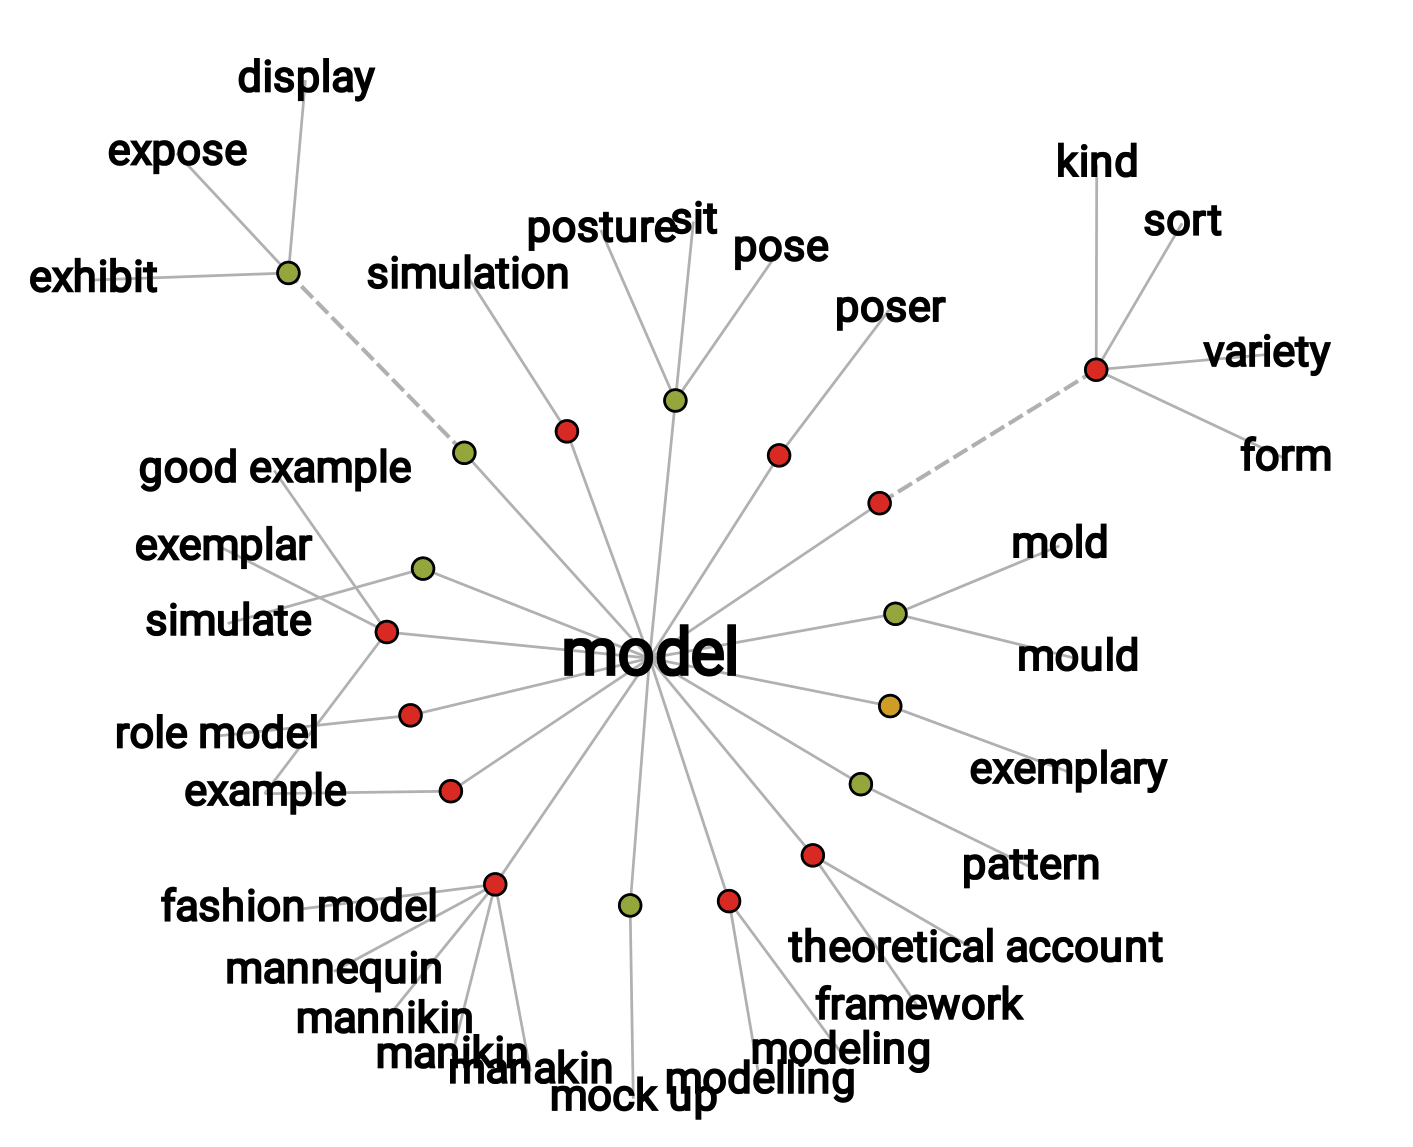
\includegraphics[width=0.9\linewidth]{fig/visualThesaurus} 

}

\caption[Network visualization of *model* thesaurus entries]{\textbf{Network visualization of
\emph{model} thesaurus entries.} Generated with the
\href{https://www.visualthesaurus.com}{`Visual Thesaurus'} ressource}\label{fig:visual-thesaurus}
\end{figure}





The narrower perspective of the scientist does not reduce the
completeness of the dictionary's description to an unambiguous object
\citep{bailer2002scientists}. In an attempt to approach these
multi-faceted objects that are the models, Daniela Bailer-Jones
interviewed different scientists and asked them the same question: what
is a model? Across the different profiles and fields of study, the
answers vary but some patterns begin to emerge (Figure
\ref{fig:interviews}). A model must capture the essence of the
phenomenon being studied. Because it eludes, voluntarily or not, many
details or complexity, it is by nature a simplification of the
phenomenon. These limitations may restrict its validity to certain cases
or suspend it to the fulfilment of some hypotheses. They are not
necessarily predictive, but they must be able to generate new
hypotheses, be tested and possibly questioned. Finally, and
fundamentally, they \textbf{must provide insights about the object of
study and contribute to its understanding}.

\begin{figure}

{\centering 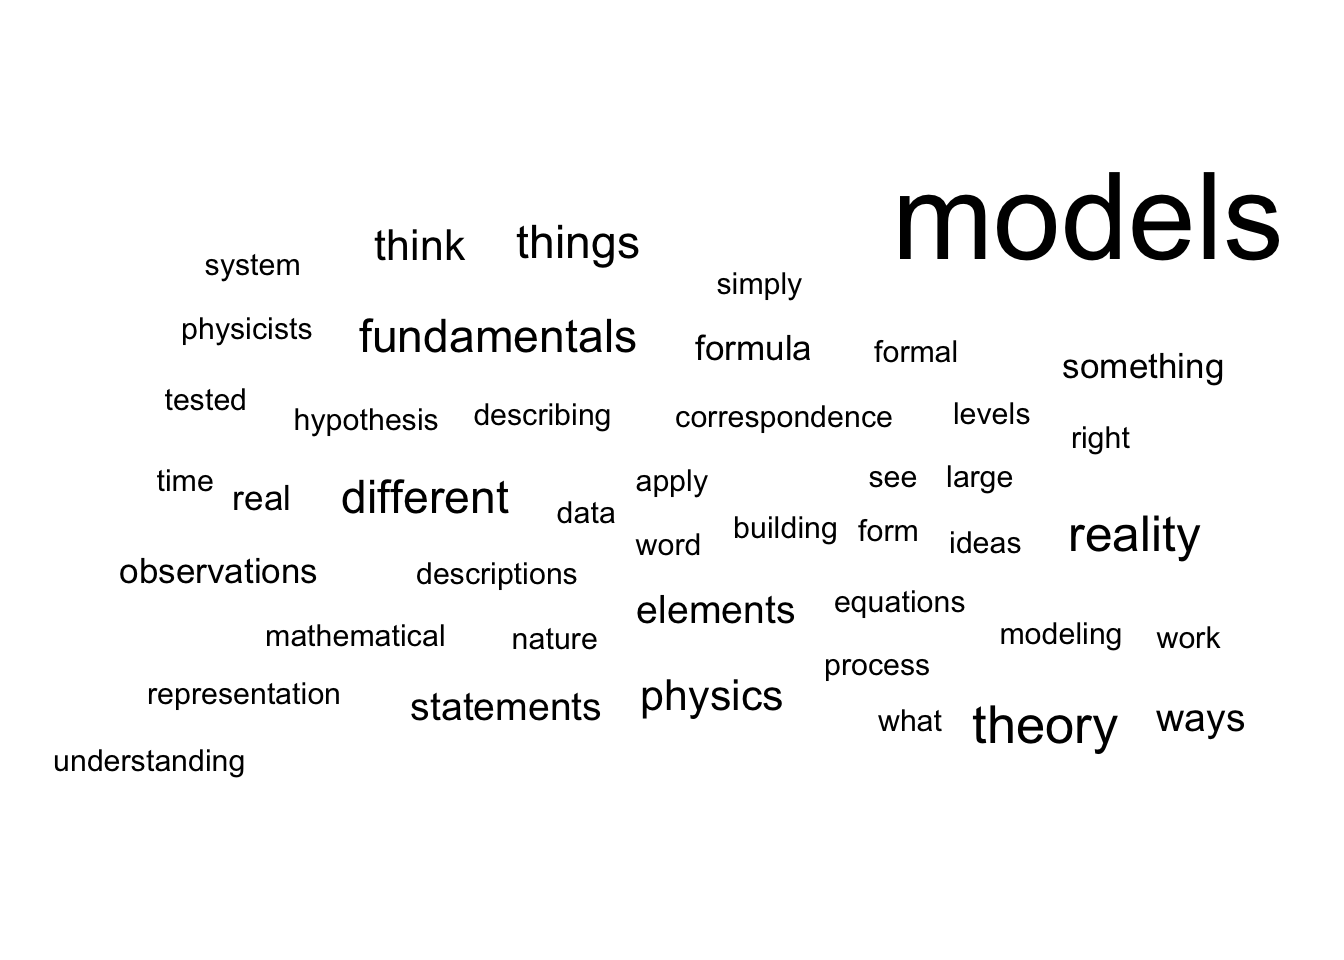
\includegraphics[width=0.9\linewidth]{01-Models_files/figure-latex/interviews-1} 

}

\caption[Scientists talk about their models: words cloud.]{\textbf{Scientists talk about their models:
words cloud.} Cloud of words summarizing the lexical fields used by
scientists to talk about their models in dedicated interviews reported
by \citet{bailer2002scientists}.}\label{fig:interviews}
\end{figure}






These definitions circumscribe the \emph{model} object, its use and its
objectives, but they do not in any way describe its nature. And for good
reason, because even if we agree on the described contours, the
biodiversity of the models remains overwhelming for taxonomists:

\begin{quote}
\emph{Probing models, phenomenological models, computational models,
developmental models, explanatory models, impoverished models, testing
models, idealized models, theoretical models, scale models, heuristic
models, caricature models, exploratory models, didactic models, fantasy
models, minimal models, toy models, imaginary models, mathematical
models, mechanistic models, substitute models, iconic models, formal
models, analogue models, and instrumental models are but some of the
notions that are used to categorize models.}\\
\citep{frigg2020models}
\end{quote}

\subsection{Physical world and world of
ideas}\label{physical-world-and-world-of-ideas}

Without claiming to be exhaustive, we can make a \textbf{first simple
dichotomy between physical/material and formal/intellectual models}
\citep{rosenblueth1945role}. The former consist in replacing the object
of study by another object, just as physical but nevertheless simpler or
better known. These may be models involving a change of scale such as
the simple miniature replica placed in a wind tunnel, or the metal
double helix model used by Watson and Crick to visualize DNA. In all
these cases the model allows to visualize the object of study (Figure
\ref{fig:planets} A and B), to manipulate it and play with it to better
understand or explain a phenomenon, just like the scientist with his
orrery (Figure \ref{fig:orrery}). In the case of biology, there are
mainly model organisms such as drosophila, zebrafish or mice, for
example. We then benefit from the relative simplicity of their genomes,
a shorter time scale or ethical differences, usually to elucidate
mechanisms of interest in humans. Correspondence between the target
system and its model can sometimes be more conceptual, such as that ones
relying on mechanical--electrical analogies: a mechanical system (e.g.~a
spring-mass system) can sometimes be represented by an electric network
(e.g.~a RLC circuit with a resistor, a capacitor and an inductor).

\begin{figure}

{\centering 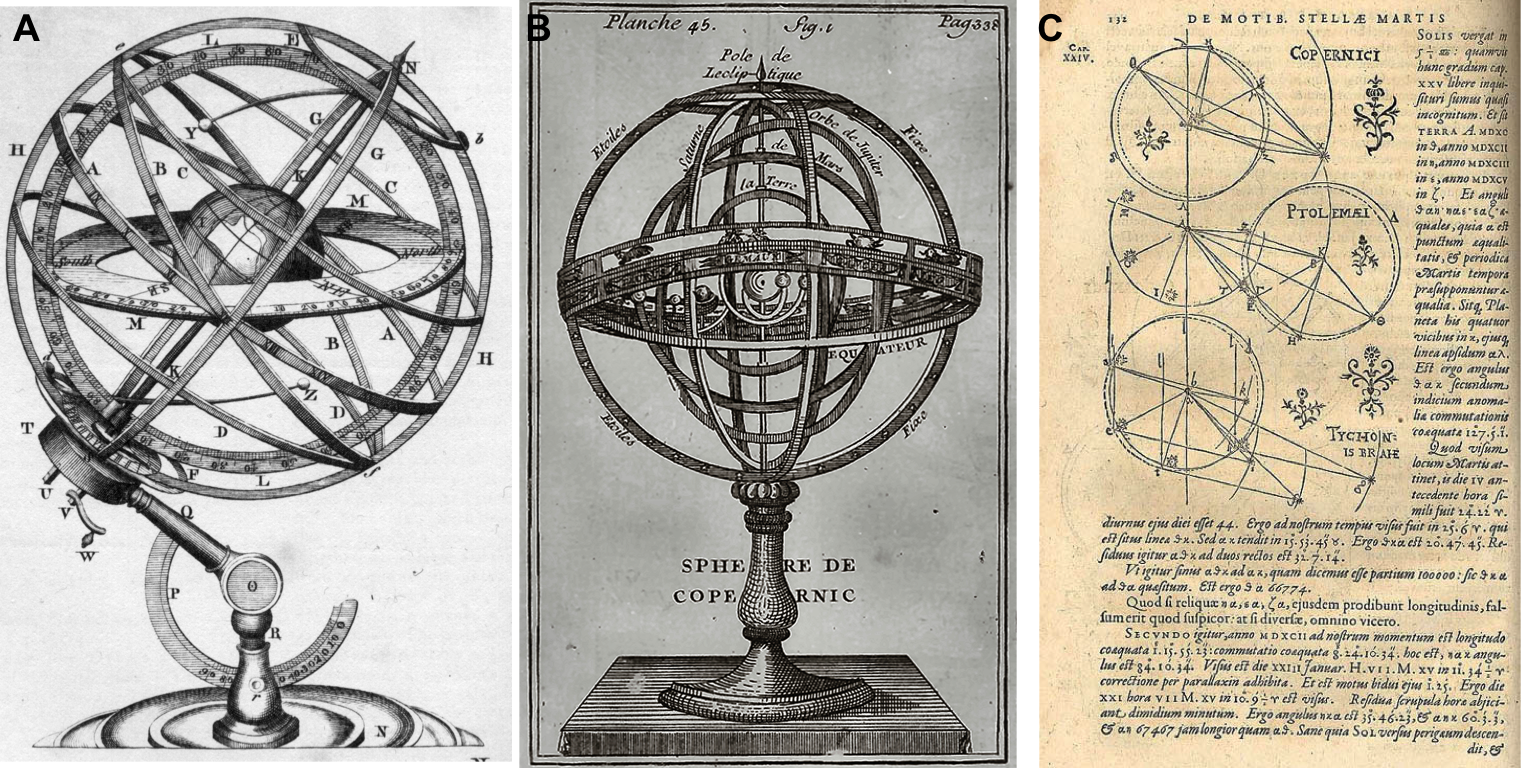
\includegraphics[width=0.9\linewidth]{01-Models_files/figure-latex/planets-1} 

}

\caption[Orrery, planets and models]{\textbf{Orrery, planets and models}. Physical
models of planetary motion, either geocentric (Armillary sphere from
\emph{Plate LXXVII} in
\href{https://commons.wikimedia.org/wiki/File:EB1711_Armillary_Sphere.png}{\emph{Encyclopedia
Britannica}}, 1771) or heliocentric in panel B (Bion, 1751,
\href{https://gallica.bnf.fr/ark:/12148/btv1b2600252q/f8.item.r=Bion}{catalogue
Bnf}) and some geometric representations by Johannes Kepler in panel C
(in
\href{https://commons.wikimedia.org/wiki/File:Kepler_astronomia_nova.jpg}{\emph{Astronomia
Nova}}, 1609)}\label{fig:planets}
\end{figure}












The model is then no longer simply a mimetic replica but is based on an
intellectual equivalence: we are gradually moving into the realm of
formal models \citep{rosenblueth1945role}. These are of a more symbolic
nature and they \textbf{represent the original system with a set of
logical or mathematical terms}, describing the main driving forces or
similar structural properties as geometrical models of planetary motions
summarized by Kepler in Figure \ref{fig:planets}C. Historically these
models have often been expressed by sets of mathematical equations or
relationships. Increasingly, these have been implemented by computer.
Despite their sometimes less analytical and more numerical nature, many
so-called computational models could also belong to this category of
formal models. There are then many formalisms, discrete or continuous,
deterministic or stochastic, based on differential equations or Boolean
algebra \citep{fowler1997mathematical}. Despite their more abstract
nature, they offer similar scientific services: it is possible to play
with their parameters, specifications or boundary conditions in order to
better understand the phenomenon. One can also imagine these formal
models from a different perspective, which starts from the data in a
bottom-up approach instead of starting from the phenomenon in a top-down
analysis. These models will then often be called statistical models or
models of data \citep{frigg2020models}. This distinction will be further
clarified in section \ref{stat-mech}.

To summarize and continue a little longer with the astronomical
metaphor, the study of a particularly complex system (the solar system)
can be broken down into a variety of different models. Physical and
mechanical models such as armillary spheres (\ref{fig:planets}A and B)
make it possible to touch the object of study. In addition, we can
observe the evolution of models which, when confronted with data, have
progressed from a geocentric to a heliocentric representation to get
closer to the current state of knowledge. Sometimes, models with more
formal representations are used to give substance to ideas and
hypotheses (\ref{fig:planets}C). One of the most conceptual forms is
then the mathematical language and one can thus consider that the
previously mentioned astronomical models find their culmination in
Kepler's equations about orbits, areas and periods that describe the
elliptical motion of the planets. We refer to them today as Kepler's
laws. The model has become a law and therefore a paragon of mathematical
modeling \citep{wan2018mathematical}.

\subsection{Preview about cancer
models}\label{preview-about-cancer-models}

As we get closer to the subject of our study, and in order to illustrate
these definitions more concretely, we can take an interest in the
meaning of the word \emph{model} in the context of cancer research. For
this, we restrict our corpus to scientific articles found when searching
for ``cancer model'' in the PubMed article database. Among these, we
look at the occurrences of the word \emph{model} and the sentences in
which it is included. This cancer-related context of model is
represented as a tree in Figure \ref{fig:pubmed-tree}. Some of the
distinctions already mentioned can be found here. The \emph{mouse} and
\emph{xenograft} models, which will be discussed later in this thesis,
represent some of the most common physical models in cancer studies.
These are animal models in which the occurrence and mechanisms of
cancer, usually induced by the biologist, are studied. On the other
hand, \emph{prediction}, \emph{prognostic} or \emph{risk score} models
refer to formal models and borrow from statistical language.

\begin{figure}

{\centering 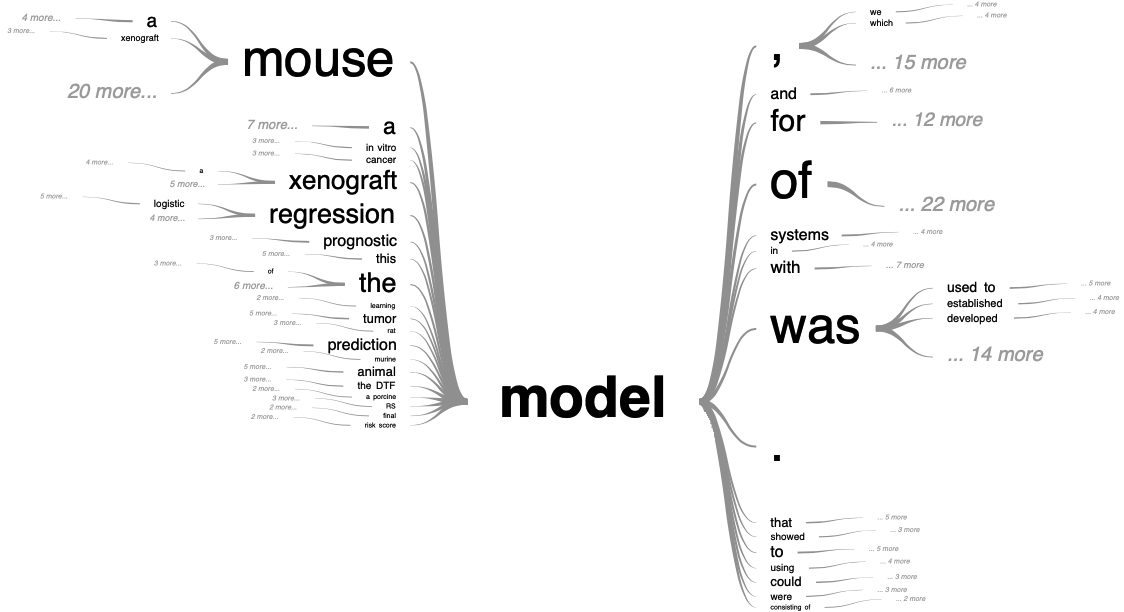
\includegraphics[width=0.9\linewidth]{fig/pubmed-tree} 

}

\caption[Tree visualization of *model* semantic context in cancer-related literature]{\textbf{Tree visualization of \emph{model}
semantic context in cancer-related literature} Generated with the
\href{https://esperr.github.io/pub-trees/}{`PubTrees'} tool by Ed Sperr,
and based on most relevant PubMed entries for ``cancer model'' search.}\label{fig:pubmed-tree}
\end{figure}






Another way to classify cancer models may be to group them into the
following categories: \emph{in vivo}, \emph{in vitro} and \emph{in
silico}. The first two clearly belong to the physical models but one
uses whole living organisms (e.g.~a human tumour implanted in an
immunodeficient mouse) and the other separates the living from its
organism in order to place it in a controlled environment (e.g.~tumour
cells in growth medium in a Petri dish). \textbf{In the thesis, data
from both \emph{in vivo} and \emph{in vitro} models will be used.
However, unless otherwise stated, a model will always refer to a
representation \emph{in silico}.} This third category, however, contains
a very wide variety of models \citep{deisboeck2009silico}, to which we
will come back in chapter \ref{mechanistic-cancer}. A final ambiguity
about the nature of the formal models used in this thesis needs to be
clarified beforehand.

\section{Statistics or mechanistic}\label{stat-mech}

A rather frequent metaphor is to compare formal models to black boxes
that take in input \(X\) predictors, or independent variables, and
output response variable(s) \(Y\), also named dependent variables. The
models then split into two categories (Figure \ref{fig:boxes}) depending
on the answer to the question: are you modeling the inside of the box or
not?

\subsection{The inside of the box}\label{the-inside-of-the-box}

The purpose of this section is to present in a schematic, and therefore
somewhat caricatural, manner the two competing formal modeling
approaches that will be used in this thesis and that we will call
mechanistic modeling and statistical modeling. Assuming the unambiguous
nature of the predictors and outputs we can imagine that the natural
process consists in defining the result Y from the inputs X according to
a function of a completely unknown form (Figure \ref{fig:boxes}A).

\begin{figure}

{\centering 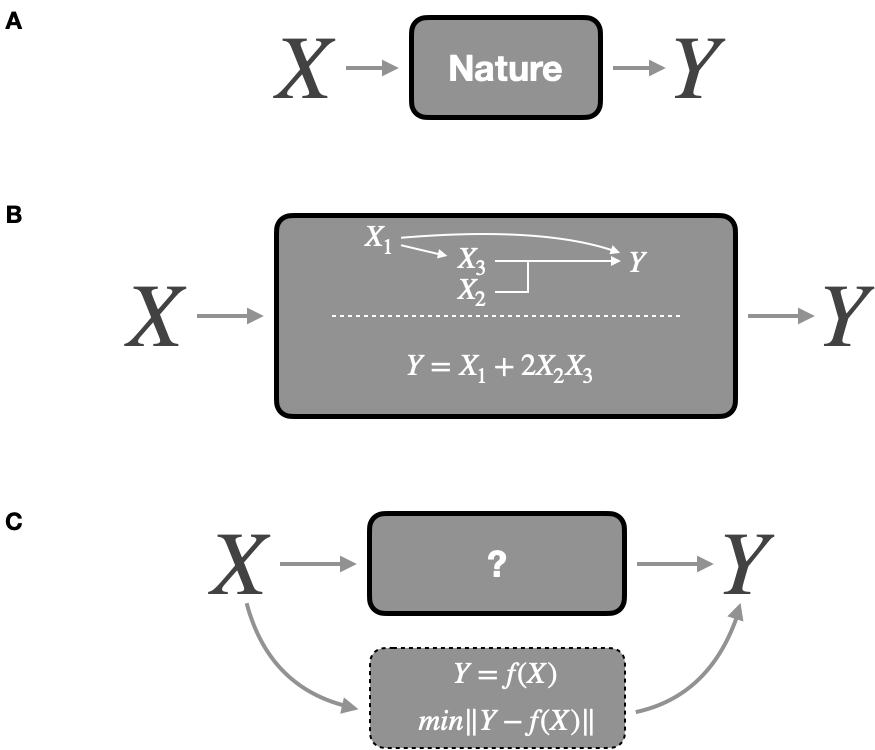
\includegraphics[width=0.6\linewidth]{fig/boxes} 

}

\caption[Different modeling strategies.]{\textbf{Different modeling strategies.} (A) Data
generation from predictors \(X\) to response \(Y\) in the natural
phenomenon. (B) Mechanistic modeling defining mechanisms of data
generation inside the box. (C) Statistical modeling finding the function
\(f\) that gives the best predictions. Aadapted from
\citet{breiman2001statistical}.}\label{fig:boxes}
\end{figure}








The first modeling approach, that we will call \textbf{mechanistic},
consists in \textbf{building the box by imitating what we think is the
process of data generation} (Figure \ref{fig:boxes}B). This integration
of a priori knowledge can take different forms. In this thesis it will
often come back to presupposing certain relations between entities
according to what is known about their behaviour. \(X_1\) which acts on
\(X_3\) may correspond to the action of one biological entity on
another, supposedly unidirectional; just as the joint action of \(X_2\)
and \(X_3\) may reflect a known synergy in the expression of genes or
the action of proteins. Mathematically this is expressed here with a
perfectly deterministic model defined a priori. All in all, in a purely
mechanistic approach, the nature of the relations between entities
should be linked to biological processes and the parameters in the model
all have biological definitions in such a way that it could even be
considered to measure them directly. For example, the coefficient \(2\)
multiplying \(X_2X_3\) can correspond to a stoichiometric coefficient or
a reaction constant which have a theoretical justification or are
accessible by experimentation. In some fields of literature these models
are sometimes called mathematical models because they propose a
mathematical translation of a phenomenon, which does not start from the
data in a bottom-up approach but rather from a top-down theoretical
framework. In this thesis we will adhere to the \emph{mechanistic model}
name, which is more transparent and less ambiguous compared to other
approaches also based on mathematics, without necessarily the other
characteristics described above.

The second approach, often called \textbf{statistical modeling}, or
sometimes machine learning depending on the precise context and
objective, does not necessarily seek to reproduce the natural process of
data generation but to \textbf{find the function allowing the best
prediction of \(Y\) from \(X\)} (Figure \ref{fig:boxes}C). Pushed to the
limit, they are ``idealized version of the data we gain from immediate
observation'' \citep{frigg2020models}, thus providing a phenomenological
description. The methods and algorithms used are then intended to be
sufficiently flexible and to make the fewest possible assumptions about
the relationships between variables or the distribution of data. Without
listing them exhaustively, the approaches such as support vector
machines \citep{cortes1995support} or random forests
\citep{breiman2001random}, which will sometimes be mentioned in this
thesis, fall into this category which contains many others
\citep{hastie2009elements}.

Several discrepancies result from this difference in nature between
mechanistic and statistical models, some of which are summarized in the
Table \ref{tab:mechstat}. In a somewhat schematic way, we can say that
the mechanistic model first asks the question of \emph{how} and then
looks at the result for the output. The \textbf{notion of causality is
intrinsic to the definition of the model}. Conversely, the statistical
model first tries to approach the Y and then possibly analyses what can
be deduced from it, regarding the importance of the variables or their
relationships in a \emph{post hoc} approach
\citep{ishwaran2007variable, manica2019toward}. The causality is then
not a by-product of the algorithm and must be evaluated with dedicated
frameworks \citep{hernan2020causal}. The greater flexibility of
statistical methods makes it possible to better accept the heterogeneity
of the variables, but this is generally done at the cost of a larger
number of parameters and therefore requires more data. Moreover,
statistical models can be considered as inductive, since they are able
to use already generated data to identify patterns in it. Conversely,
mechanistic models are more deductive in the sense that they can
theoretically allow to extrapolate beyond the original data or knowledge
used to build the model \citep{baker2018mechanistic}. Finally, the most
relevant way of assessing the value or adequacy of these models may be
quite different. A statistical model is measured by its ability to
predict output in a validation dataset different from the one used to
train its parameters. The mechanistic model will also be evaluated on
its capacity to approach the data but also to order it, to give a
meaning. If its pure predictive performance is generally inferior,
\textbf{how can the value of understanding be assessed?} This question
will be one of the threads of the dissertation.

\begin{table}

\caption{\label{tab:mechstat}\textbf{Some pros and cons for mechanistic and
statistical modeling}. Adapted from \citet{baker2018mechanistic}.}
\centering
\begin{tabular}[t]{>{\raggedright\arraybackslash}p{15em}||>{\raggedright\arraybackslash}p{15em}}
\hline
\rowcolor[HTML]{808080}  \multicolumn{1}{>{\centering\arraybackslash}p{15em}}{\textcolor{white}{\textbf{Mechanistic modeling}}} & \multicolumn{1}{>{\centering\arraybackslash}p{15em}}{\textcolor{white}{\textbf{Statistical modeling}}}\\
\hline
\multicolumn{2}{l}{\textbf{Definition}}\\
\hline
\hspace{1em}Seeks to establish a mechanistic relationship between inputs and outputs & Seeks to establish statistical relationships between inputs and outputs\\
\hline
\multicolumn{2}{l}{\textbf{Pros and cons}}\\
\hline
\hspace{1em}Presupposes and investigates causal links between the variables & Looks for patterns and establishes correlations between variables\\
\hline
\hspace{1em}Capable of handling small datasets & Requires large datasets\\
\hline
\hspace{1em}Once validated, can be used as a predictive tool in new situations possibly difficult to access through experimentation & Can only make predictions that relate to patterns within the data supplied\\
\hline
\hspace{1em}Difficult to accurately incorporate information from multiple space and time scales due to constrained specifications & Can tackle problems with multiple space and time scales thanks to flexible specifications\\
\hline
\hspace{1em}Evaluated on closeness to data and ability to make sense of it & Evaluated based on predictive performance\\
\hline
\end{tabular}
\end{table}




Mechanistic and statistical models are not perfectly exclusive and
rather form the two ends of a spectrum. The definitions and
classification of some examples is therefore still partly personal and
arbitrary. For instance, the example in \ref{fig:boxes}B can be
transformed into a model with a more ambiguous status:

\[logit(P[Y=1])=\beta_1X_1 + \beta_{23}X_2X_3\]

This model is deliberately ambiguous. As a logistic model, it is
therefore naturally defined as a statistical model. But the definition
of the interaction between \(X_2\) and \(X_3\) denotes a mechanistic
presupposition. The very choice of a logistic and therefore parametric
model could also result from a knowledge of the phenomenon, even if in
practice it is often a default choice for a binary output. Finally, the
nature of the parameters \(\beta_{1}\) and \(\beta_{23}\) is likely to
change the interpretation of the model. If they are deduced from the
data and therefore optimized to fit Y as well as possible, one will
think of a statistical model whose specification is nevertheless based
on knowledge of the phenomenon. On the other hand, one could imagine
that these parameters are taken from the biochemistry literature or
other data. The model will then be more mechanistic. The boundary
between these models is further blurred by the different possibilities
of combining these approaches and making them complementary
\citep{baker2018mechanistic, salvucci2019machine}.

\subsection{A tale of prey and predators}\label{lotkasection}

The following is a final general illustration of the concepts and
procedures introduced with respect to statistical and mechanistic models
through a famous and characteristic example: the Lotka-Volterra model of
interactions between prey and predators. This model was, like many
students, my first encounter with what could be called mathematical
biology. The Italian mathematician Vito Volterra states this system for
the first time studying the unexpected characteristics of fish
populations in the Adriatic Sea after the First World War.
Interestingly, Alfred Lotka, an American physicist deduced the exact
same system independantly, starting from very generic process of
redistribution of matter among the several components derived from law
of mass action \citep{knuuttila2017modelling}. A detailed description of
their works and historical formulation can be found in original articles
\citep{lotka1925principles, volterra1926fluctuations} or dedicated
reviews \citep{knuuttila2017modelling}.

The general objective is to understand the evolution of the populations
of a species of prey and its predator, reasonably isolated from outside
intervention. Here we will use Canada lynx (\emph{Lynx canadensis}) and
snowshow hare (\emph{Lepus americanus}) populations for which an
illustrative data set exists \citep{hewitt1917conservation}. In fact,
commercial records listing the quantities of furs sold by trappers to
the Canadian Hudson Bay Company may represent a proxy for the
populations of these two species as represented in Figure
\ref{fig:lotka}A. Denoting the population of lynx \(L(t)\) and the
population of hare \(H(t)\) it can be hypothesized that prey, in the
absence of predators, would increase in population, while predators on
their own would decline in the absence of preys. A prey/predator
interaction term can then be added, which will positively impact
predators and negatively impact prey. The system can then be formalized
with the following differential questions with all coefficients
\(a_1, a_2, b_1, b_2 >0\):

\[\dfrac{dH}{dt}=a_1H-a_2HT\]

\[\dfrac{dL}{dt}=-b_1L+b_2HL\]

\(a_1H\) represents the growth rate of the hare population (prey),
i.e.~the population grows in proportion to the population itself
according to usual birth modeling. The main losses of hares are due to
predation by lynx, as represented with a negative coefficient in the
\(-a_2HT\) term. It is therefore assumed that a fixed percentage of
prey-predator encounters will result in the death of the prey.
Conversely, it is assumed that the growth of the lynx population depends
primarily on the availability of food for all lynxes, summarized in the
\(b_2HL\) term. In the absence of hares, the lynx population decreases,
as denoted by the coefficient \(-b_1L\). Important features of
mechanistic models are illustrated here: the equations are based on a
priori knowledge or assumptions about the structure of the problem and
the parameters of the model can be interpreted. \(a_1\), for example,
could correspond to the frequency of litters among hares and the number
of offspring per litter.

\begin{figure}

{\centering 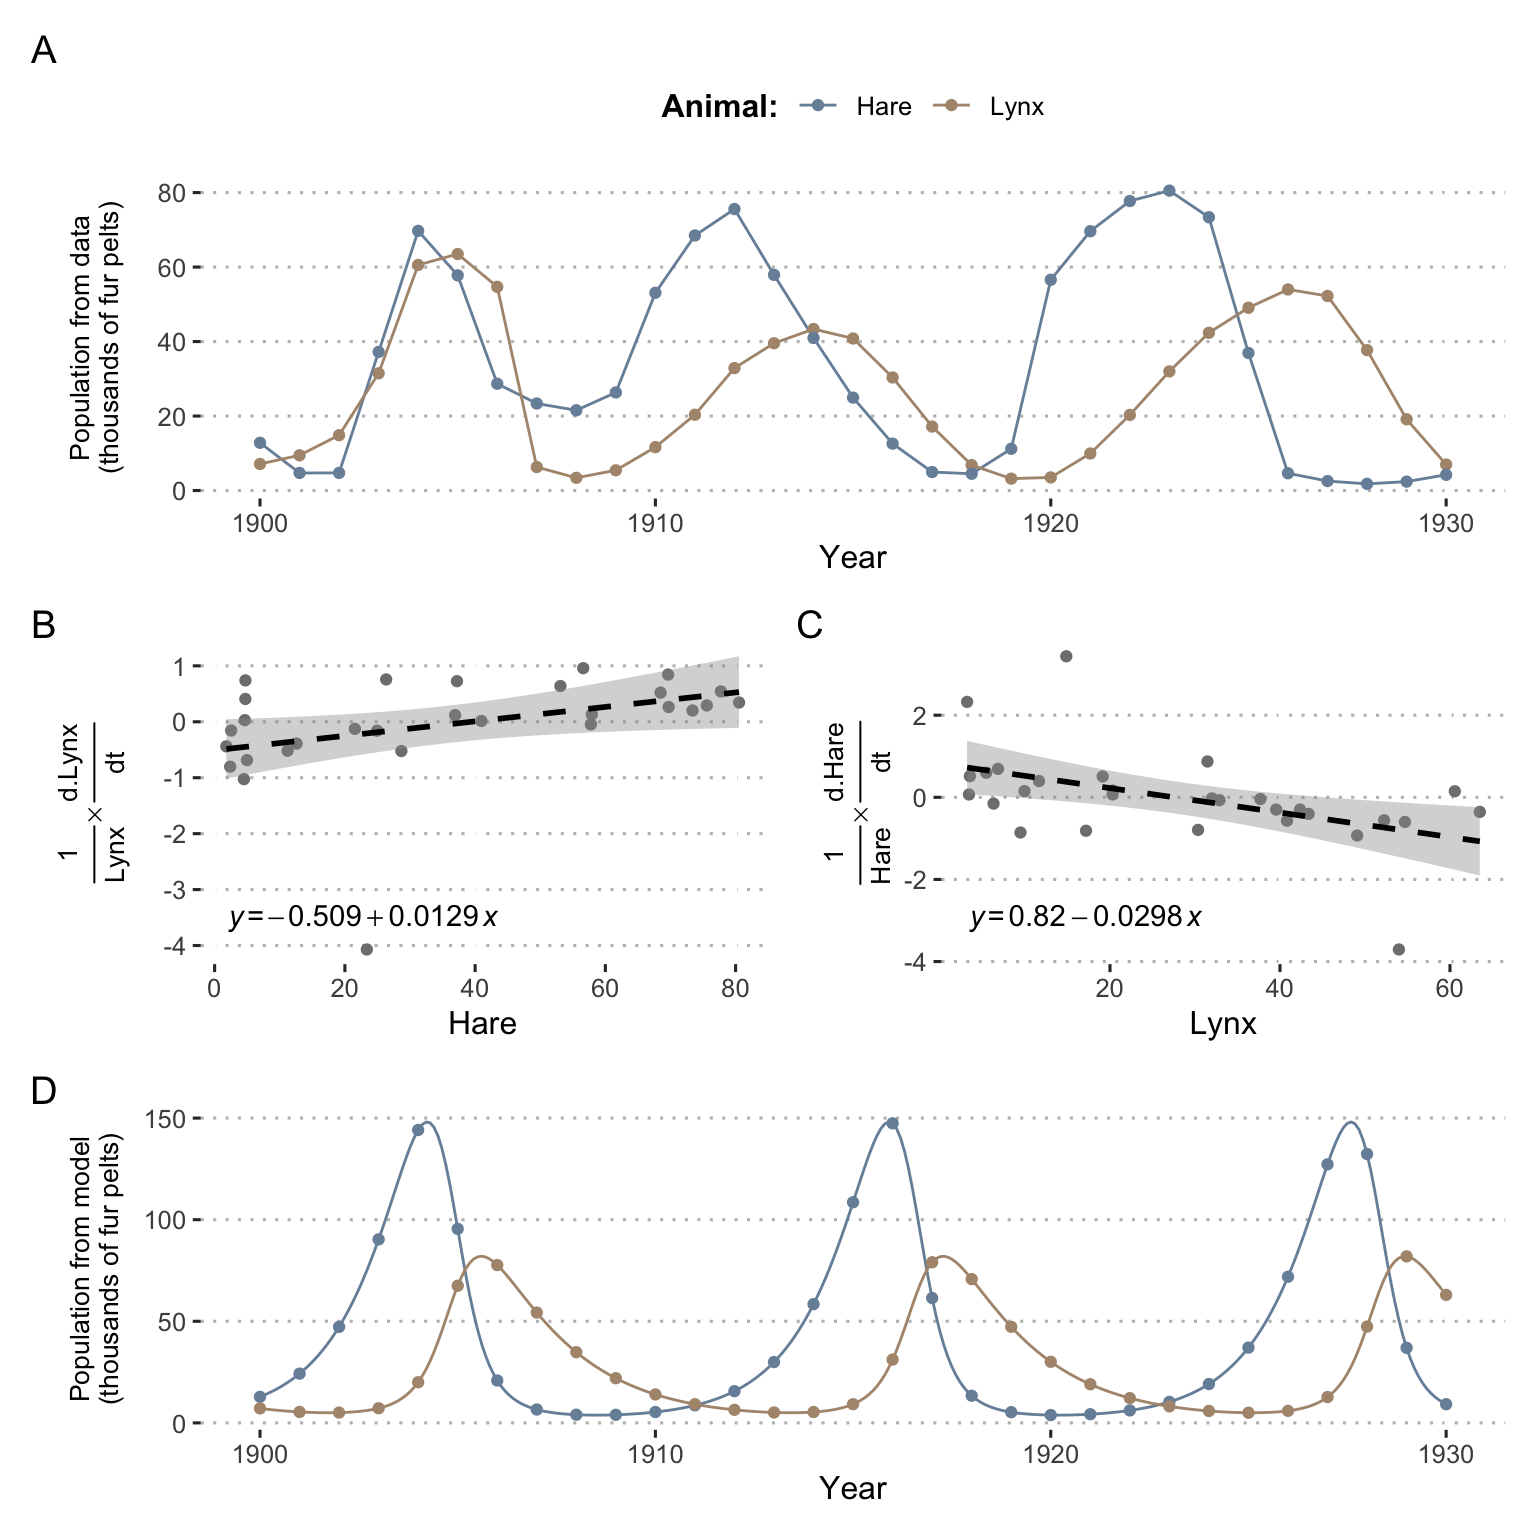
\includegraphics[width=0.9\linewidth]{01-Models_files/figure-latex/lotka-1} 

}

\caption[Some analyses around Lotka-Volterra model of a prey-predator system]{\textbf{Some analyses around Lotka-Volterra model of
a prey-predator system}. (A) Evolution of lynx and hares populations
based on Hudson Bay Company data about fur pelts. (B) and (C) Linear
regression for estimation of parameters. (D) Evolution of lynx and hare
populations as predicted by the model based on inferred parameters and
initial conditions.}\label{fig:lotka}
\end{figure}








This being said, the structure of the model having been defined a
priori, it remains to determine its parameters. Two options would
theoretically be possible: to propose values based on the interpretation
of the parameters and ecological knowledge, or to fit the model to the
data in order to find the best parameters. For the sake of simplicity,
and because this example has only a pedagogical value in this
presentation, we propose to determine them approximately using the
following Taylor-based approximation:

\[\dfrac{1}{y(t)} \dfrac{dy}{dt} \simeq \dfrac{1}{y(t)} \dfrac{y(t+1)-y(t-1)}{2}\]

By applying this approximation to the two equations of the differential
system and plotting the corresponding linear regressions (Figures
\ref{fig:lotka}B and C), we can obtain an evaluation of the parameters
such as \(a_1=0.82\), \(a_2=0.0298\), \(b_1=0.509\), \(b_2=0.0129\). By
matching the initial conditions to the data, the differential system can
then be fully determined and solved numerically (Figures
\ref{fig:lotka}D). Comparison of data and modeling provides a good
illustration of the virtues and weaknesses of a mechanistic model.
Firstly, based on explicit and interpretable hypotheses, the model was
able to recover the cyclical behaviour and dependencies between the two
species: the increase in the lynx population always seems to be preceded
by the increase in the hare population. However, the amplitude of the
oscillations and their periods are not exactly those observed in the
data. This may be related to approximations in the evaluation of
parameters, random variation in the data or, of course, simplifications
or errors in the structure of the model itself.

Besides, if one tries to carry out a statistical modeling of these data,
it is very likely that it is possible to approach the curve of
populations evolution much closer, especially for the hares. But should
it be expressed simply as a function of time or should a joint modeling
be proposed? The nature of the causal link between prey and predators
will be extremely difficult to establish without strong hypotheses such
as those of the mechanistic model. On the other hand, if populations in
later years had to be predicted as accurately as possible, it is likely
that a sufficiently well-trained statistical model would perform better.
Finally, and this is a fundamental difference, the \textbf{mechanistic
model enables to test cases or hypotheses that go beyond the scope of
the data}. Quite simply, by playing with the variables or parameters of
the model, we can predict the exponential decrease of predators in the
absence of prey and the exponential growth of prey in the absence of
prey. More generally, it is also possible to study analytically or
numerically the bifurcation points of the system in order to determine
the families of behaviours according to the relative values of the
parameters \citep{flake1998computational}. It is not possible to infer
these new or hypothetical behaviours directly from the data o of the
statistical model. This is theoretically possible on the basis of the
mechanistic model, provided that it is sufficiently relevant and that
its operating hypotheses cover the cases under investigation. Now that
the value of mechanistic models has been illustrated in a fairly
theoretical example, all that remains is to explore in the next chapters
how they can be built and used in the context of cancer.

\section{Simplicity is the ultimate
sophistication}\label{simplicity-is-the-ultimate-sophistication}

Before concluding this modeling introduction, it is important to
highlight one of the most important points already introduced in a
concise manner by the poet Paul Valéry at the beginning of this chapter.
\textbf{Whatever its nature, a model is always a simplified
representation of reality and by extension is always wrong to a certain
extent}. This is a generally well-accepted fact, but it is crucial to
understand the implications for the modeller. This simplification is not
a collateral effect but an intrinsic feature of any model:

\begin{quote}
\emph{No substantial part of the universe is so simple that it can be
grasped and controlled without abstraction. Abstraction consists in
replacing the part of the universe under consideration by a model of
similar but simpler structure. Models, formal and intellectual on the
one hand, or material on the other, are thus a central necessity of
scientific procedure.}\\
\citep{rosenblueth1945role}
\end{quote}

Therefore, a model exists only because we are not able to deal directly
with the phenomenon and simplification is a necessity to make it more
tractable \citep{potochnik2017idealization}. This simplification
appeared many times in the studies of frictionless planes or
theoretically isolated systems, in a totally deliberate strategy.
However, this idealization can be viewed in several ways
{[}weisberg2007three{]}. One of them, called Aristotelian or minimal
idealization, is to eliminate all the properties of an object that we
think are not relevant to the problem in question. This amounts to lying
by omission or making assumptions of insignificance by focusing on key
causal factors only \citep{frigg2020models}. We therefore refer to the
\emph{a priori} idea that we have of the phenomenon. The other
idealization, called Galilean, is to deliberately distort the theory to
make it tractable as explicited by Galileo himself:

\begin{quote}
\emph{We are trying to investigate what would happen to moveables very
diverse in weight, in a medium quite devoid of resistance, so that the
whole difference of speed existing between these moveables would have to
be referred to inequality of weight alone. Since we lack such a space,
let us (instead) observe what happens in the thinnest and least
resistant media, comparing this with what happens in others less thin
and more resistant.}
\end{quote}

This fairly pragmatic approach should make it possible to evolve
iteratively, reducing distortions as and when possible. This could
involve the addition of other species or human intervention into the
Lotka-Volterra system described above. A three-species Lotka-Volterra
model can however become chaotic \citep{flake1998computational}, and
therefore extremely difficult to use and interpret, thus underlining the
importance of simplifying the model.

We will have the opportunity to come back to the idealizations made in
the course of the cancer models but it is already possible to give some
orientations. The biologist who seeks to study cancer using cell lines
or animal models is clearly part of Galileo's lineage. The mathematical
or \emph{in silico} modeler has a more balanced profile. The design of
qualitative mechanistic models based on prior knowledge, which is the
core of the second part of the thesis, is more akin to minimal
idealization, which seeks to highlight the salient features of a system.
But the Galilean pragmatism consisting in creating
computationnaly-tractable models is also quite widespread, particularly
in highly dimensional statistical approaches.

Because of the complexity of the phenomena, simplification is therefore
a necessity. The objective then should not necessarily be to make the
model more complex, but to \textbf{match its level of simplification
with its assumptions and objectives}. Faced with the temptation of the
author of the model, or his reviewer, to always extend and complicate
the model, it could be replied with Lewis Carrol words\footnote{More
  concisely stated by \citet{rosenblueth1945role}: ``best material model
  for a cat is another cat, or preferably the same cat.''}:

\begin{quote}
\emph{``That's another thing we've learned from your Nation,'' said Mein
Herr, ``map-making. But we've carried it much further than you. What do
you consider the largest map that would be really useful?''}\\
\emph{``About six inches to the mile.''}\\
\emph{``Only six inches!'' exclaimed Mein Herr. ``We very soon got to
six yards to the mile. Then we tried a hundred yards to the mile. And
then came the grandest idea of all! We actually made a map of the
country, on the scale of a mile to the mile!''}\\
\emph{``Have you used it much?'' I enquired.}\\
\emph{``It has never been spread out, yet,'' said Mein Herr: ``the
farmers objected: they said it would cover the whole country, and shut
out the sunlight! So we now use the country itself, as its own map, and
I assure you it does nearly as well.''}\\
Lewis Carroll, \emph{Sylvie and Bruno} (1893)
\end{quote}

\chapter{Cancer as deregulation of complex
machinery}\label{cancer-as-deregulation-of-complex-machinery}

\epigraph{"Does not the entireness of the complex hint at the perfection of the simple?"}{Edgar Allan Poe (Eureka)}

\initial{A}rmed with all these models, whether statistical or
mechanistic, we are going to look at cancer, a particularly complex
system that fully justifies their use. Since the first chapter recalled
how important prior knowledge of the phenomenon under study is for
designing models, whatever their nature, this chapter will briefly
summarize some of the most important characteristics of this disease
before returning to the models themselves in the next chapter. Without
aiming for exhaustiveness, and after an epidemiological and statistical
description, we will focus on the most useful information for the
modeller, i.e.~the underlying biological mechanisms and available data.

\begin{figure}

{\centering 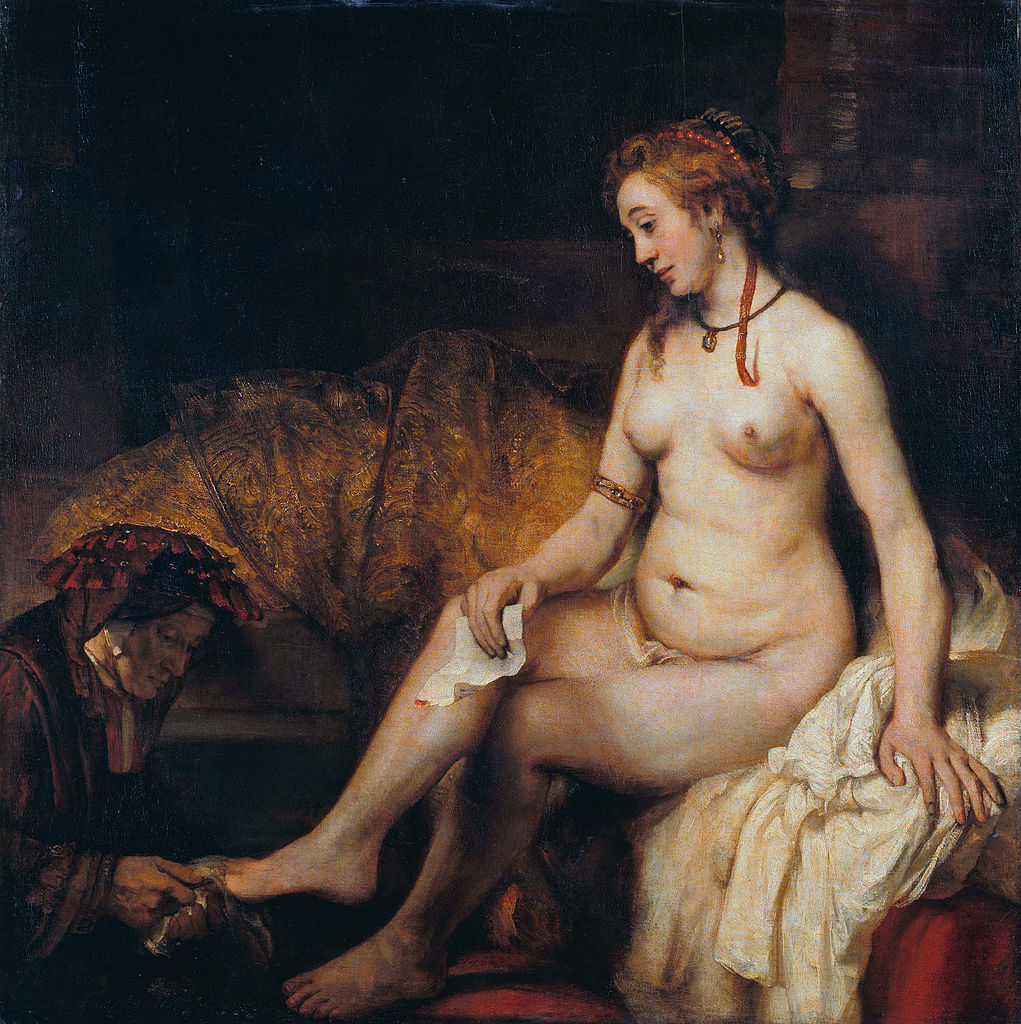
\includegraphics[width=0.9\linewidth]{fig/bath} 

}

\caption[Cancer is an old disease]{\textbf{Cancer is an old disease.} Rembrandt,
\emph{Bathsheba at Her Bath}, c. 1654, oil on canvas, Louvre Museum,
Paris}\label{fig:bath}
\end{figure}





\section{What is cancer?}\label{what-is-cancer}

Cancer can be described as a group of diseases characterized by
\textbf{uncontrolled cell divisions and growth which can spread to
surrounding tissues}. Descriptions of this disease, especially when
associated with solid tumors, have been found as far back as ancient
Egyptian documents, at least 1600 BC and we know from the first century
A.D. with Aulus Celsus that it is better to remove the tumors and this
as soon as possible \citep{hajdu2011note}. Progress will accelerate
during the Renaissance with the renewed interest in medicine, and
anatomy in particular, which will advance the knowledge of tumor
pathology and surgery \citep{hajdu2011note2}. The progress of anatomical
knowledge has also left brilliant testimonies in the field of painting,
which make the renown of the Renaissance today. The precision of these
artists' traits has also allowed some retrospective medical analyses,
some of them going so far as to identify the signs of a tumor in some of
the subjects of these paintings \citep{bianucci2018earliest}. Such is
the bluish stain on the left breast of the Bathsheba painted by
Rembrandt (Figure \ref{fig:bath}) which has been subject to
controversial interpretations, sometimes described as an example of
``skin discolouration, distortion of symmetry with axillary fullness and
peau d'orange'' \citep{braithwaite1983rembrandt} and sometimes spared by
photonic and computationnal analyses \citep{heijblom2014monte}. The
mechanisms of the disease only began to be elucidated with the
appearance of the microscope in the 19th century, which revealed its
cellular origin \citep{hajdu2012note}. The classification and
description of cancers is then gradually refined and the first
non-surgical treatments appear with the discovery of ionising radiation
by the Curies \citep{hajdu2012note2}. The 20th century is then the
century of understanding the causes of cancer
\citep{hajdu2013note, hajdu2013note2}. Some environmental exposures are
characterized as asbestos or tobacco. Finally, the biological mechanisms
become clearer with the identification of tumor-causing viruses and
especially with the discovery of DNA \citep{watson1953molecular}. The
foundations of our current understanding of cancer date back to this
period, which marks the beginning of the molecular biology of cancer. It
is this branch of biology that contains the bulk of the knowledge that
will be used to build our mechanistic models, and it will be later
detailed in Section \ref{molecular-biology}.

One of the ways to read this brief history of cancer is to see that
theoretical and clinical progress has not followed the same
timeframes.The medical and clinical management of cancers initially
progressed slowly but surely, and this in the absence of an
understanding of the mechanisms of cancer. Conversely, the theoretical
progress of the last century has not always led to parallel medical
progress, except on certain specific points. The interaction between the
two is therefore not always obvious. The \textbf{transformation of
fundamental knowledge into medical and clinical impact is therefore of
particular importance}. This is what is called \emph{translational
medicine}, the aim of which is to go from laboratory bench to bedside
\citep{cohrs2015translational}. It is in this perspective that we will
analyze the mechanistic models studied in this thesis. Their objective
is to integrate biological knowledge, or at least a synthesis this
knowledge, in order to transform it into a relevant clinical
information.

\section{Cancer from a distance: epidemiology and main
figures}\label{epidemio}

Before going down to the molecular level, it is important to detail some
figures and trends in the epidemiology of cancer today. Following the
description in the previous section, cancer is first and foremost
defined as a disease. Considered to be a unique disease, it caused 18.1
million new cancer cases and 9.6 million cancer deaths in 2018 according
to the Global Cancer Observatory affiliated to World Health Organization
\citep{bray2018global}. However, these aggregated data conceal
disparities of various kinds. The first one is geographical. Indeed,
mortality figures make cancer one of the leading causes of premature
death in most countries of the world but its importance relative to
other causes of death is even greater in the more developed countries
(Figure \ref{fig:globocan-map}). All in all, cancer is the first or
second cause of premature death in almost 100 countries worldwide
\citep{bray2018global}. These differences call for careful consideration
of the impact of population age structures and health-related
covariates.

\begin{figure}

{\centering 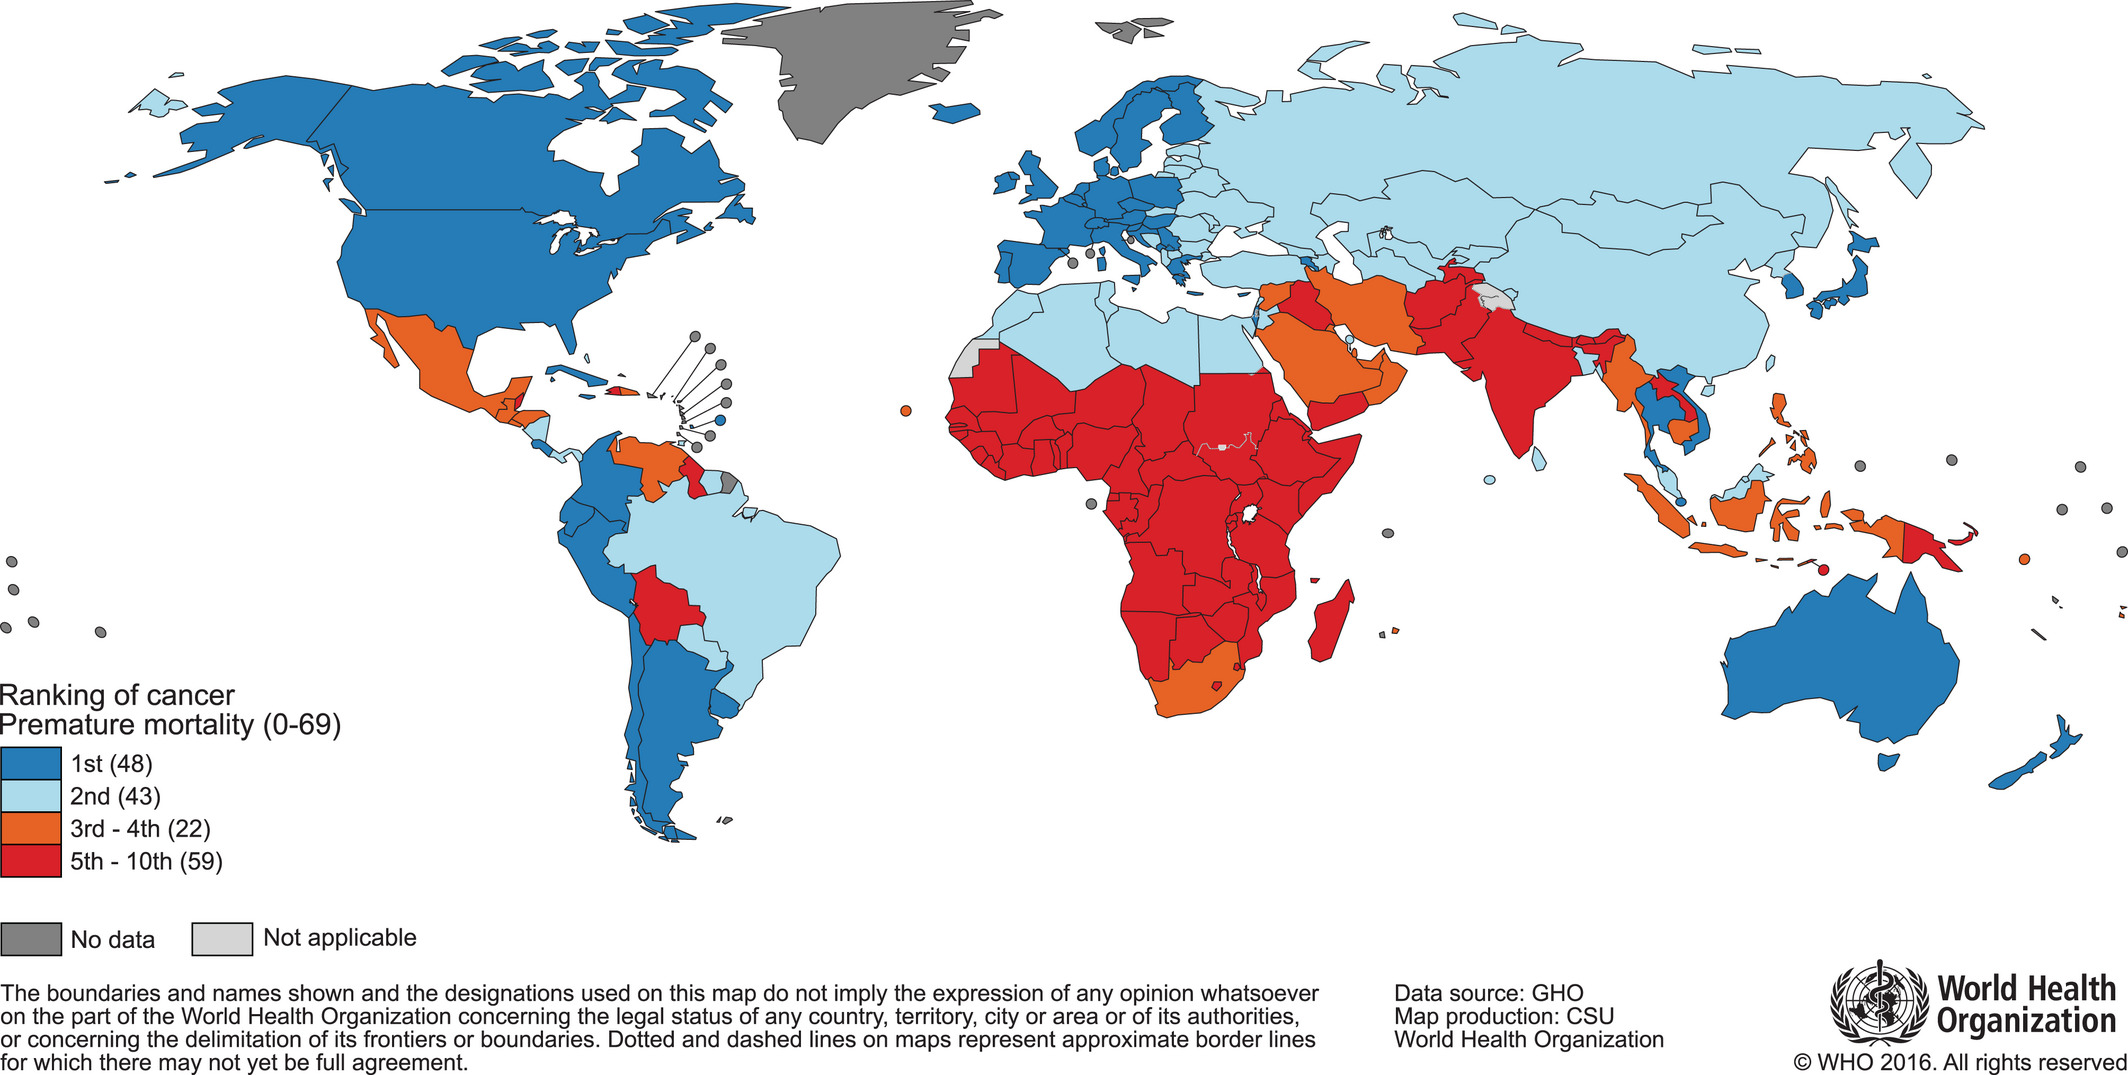
\includegraphics[width=0.9\linewidth]{fig/globocan-map} 

}

\caption[World map and national rankings of cancer as a cause of premature death]{\textbf{World map and national rankings of
cancer as a cause of premature death.} Classification of cancer as a
cause of death before the age of 70, based on data for the year 2015.
Original Figure, data and methods from \citet{bray2018global}.}\label{fig:globocan-map}
\end{figure}






A second disparity lies in the different types of cancer. If we classify
tumors solely according to their location, i.e.~the organ affected
first, we already obtain very wide differences. First of all, the
incidence varies considerably (Figure \ref{fig:cancer-tissues}A)).
Cancers do not occur randomly anywhere in the body and certain
environments or cell types appear to be more favourable
\citep{tomasetti2015variation}. Mortality is also highly variable but is
not directly inferred from incidence. Not all types of cancer have the
same prognosis (Figure \ref{fig:cancer-tissues}A and B) and survival
rates \citep{liu2018integrated}. Although breast cancer is much more
common than lung cancer, it causes fewer deaths because its prognosis
is, on average, much better. The mechanisms at work in the emergence of
cancer are therefore not necessarily the same as those that will govern
its evolution or its response to treatment. And still on the response to
treatment, Figure \ref{fig:cancer-tissues}B highlights another
disparity: not only are the survival prognosis associated with each
cancer very different, but the evolution (and generally the improvement)
of these prognoses has been very uneven over the last few decades. This
means that theoretical and therapeutic advances have not been applied to
all types of cancer with the same success. It is one more indication of
the \textbf{diversity of cancer mechanisms in different tissues and
biological contexts}, which make it impossible to find a panacea, and
which, on the contrary, encourage us to carefully consider the
particularities of each tumor, both to understand them and to treat
them. Under a generic name and in spite of common characteristics, the
cancers thus appear as extremely heterogeneous. And to understand the
sources of this heterogeneity, it is necessary to consider the disease
on a smaller scale.

\begin{figure}

{\centering 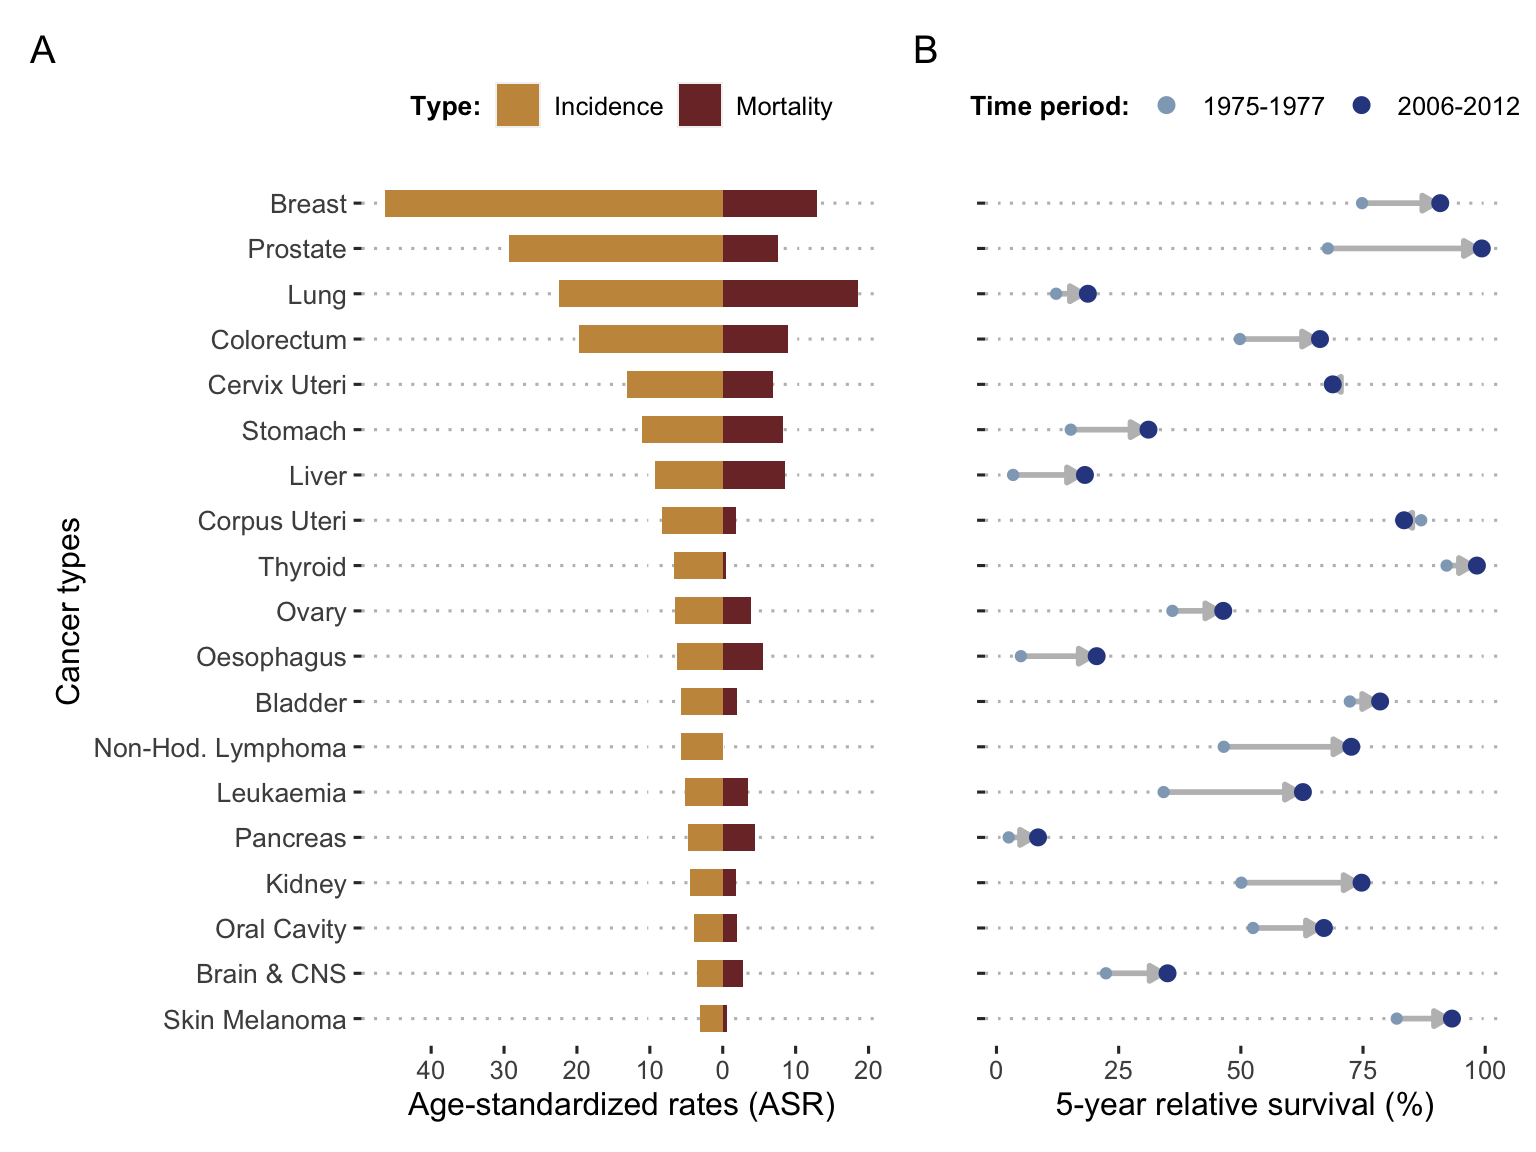
\includegraphics[width=0.9\linewidth]{02-Cancer_files/figure-latex/cancer-tissues-1} 

}

\caption[Incidence, mortality and survival per cancer types]{\textbf{Incidence, mortality and survival
per cancer types}. (A) World incidence and mortality for the 19 most
frequent cancer types in 2018, expressed with age-standardized rates
(adjusted age structure based on world population); data retrieved from
\href{https://gco.iarc.fr/today/home}{Global Cancer Observatory}. (B)
Evolution of 5-years relative survival for the same cancer types based
on US data from SEER registries in 1975-1977 and 2006-2012; data
retrieved from \citet{jemal2017annual}.}\label{fig:cancer-tissues}
\end{figure}










\section{Basic molecular biology and cancer}\label{molecular-biology}

If it is not possible and desirable to summarize here the state of
knowledge about the biology of cancer, we are going to give a very
partial vision focused on the main elements used in this thesis, thus
aiming to make it a self-sufficient document. The details necessary for
a finer and more general understanding can be found in dedicated
textbooks such as \citet{alberts2007molecular} and
\citet{weinberg2013biology}.

\subsection{Central dogma and core
principles}\label{central-dogma-and-core-principles}

Some of the principles that govern biology can be described at the level
of one of its simplest element, the cell. Let us consider for the moment
a perfectly healthy cell. It must ensure a certain number of functions
necessary for its survival and, if necessary, for its
division/reproduction. These functions are encoded in its genetic
information in the form of DNA, which is stable and shared by the
different cells since it is defined at the level of the individual. Most
biological functions, however, are not performed by DNA itself which
remains in the nucleus of the cell. The DNA is thus transcribed into
RNA, another nucleic acid which, in addition to performing some
biological functions, becomes the support of the genetic information in
the cell. The RNA is then itself translated into new molecules composed
of long chains of amino acid residues and called proteins. They are the
ones that execute most of the numerous cellular functions: DNA
replication, physical structuring of the cell, molecule transport within
the cell etc. A rather simplistic but fruitful way to understand this
functioning is to consider it as a \textbf{progressive transfer of
biological information from DNA to proteins}, which has sometimes been
summarized as the central dogma of the molecular biology
(\ref{fig:central-dogma}), first stated Francis Crick
\citep{crick1970central}.

\begin{figure}

{\centering 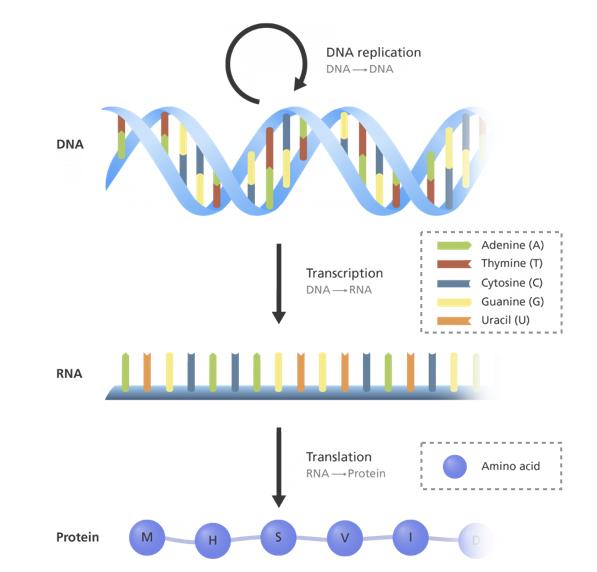
\includegraphics[width=0.8\linewidth]{fig/central-dogma} 

}

\caption[Central dogma of molecular biology]{\textbf{Central dogma of molecular biology.}
Schematic representation of the information flow within the cell, from
DNA to proteins through RNA, more precisely described in this
\href{https://www.youtube.com/watch?v=J3HVVi2k2No}{video} (Image credit
\emph{Genome Research Limited}).}\label{fig:central-dogma}
\end{figure}







However, many changes would be necessary to clarify this scheme and the
uni-directional nature was questioned early on. Above all, a large
number of regulations interact with and disrupt this master plan. The
genes are not always all transcribed, or at least not at constant
intensities, interrupting or varying the chain upstream. This modulation
in the transcription of genes can be induced by proteins, called
transcription factors. After a gene transcription, its expression can
still be regulated at various stages. RNAs can also be degraded more or
less rapidly. RNAs can be reshaped in their structure by a process
called splicing, which varies the genetic information they carry.
Finally, proteins are subject to all kinds of modifications referred to
as post-translational, which can change the chemical nature of certain
groups or modify the three-dimensional structure of the whole protein.
For instance, some proteins perform their function only if a specific
amino acid residue is phosphorylated. In addition, these modifications
can be transmitted between proteins, further complicating the flow of
information. \textbf{All these possibilities of regulation play an
absolutely essential role in the life of the cell by allowing it to
adapt to different contexts and situations}. From the same genetic
material, a cell of the eye and a cell of the heart can thus perform
different functions. Similarly, the same cell subjected to different
stimuli at different times can provide different responses because these
molecular stimuli trigger a regulation of its programme. But all these
regulatory mechanisms can be corrupted.

\subsection{A rogue machinery}\label{a-rogue-machinery}

With the above knowledge we can now return to the definition of cancer
as an uncontrolled division of cells that can lead to the growth of a
tumor that eventually spreads to the surrounding tissues. Therefore,
this corresponds to normal processes, like cell division and
reproduction, that are no longer regulated as they should be and are out
of control. Experiments on different model organisms have gradually
identified genetic mutations as a major source of these deregulations
\citep[\citet{reddy1982point}]{nowell1976clonal} until cancer was
clearly considered as a \textbf{genetic disease} making Renato Dulbecco,
Nobel Laureate in Medicine for his work on oncoviruses, say:

\begin{quote}
\emph{If we wish to learn more about cancer, we must now concentrate on
the cellular genome.}\\
\citep{dulbecco1986turning}.
\end{quote}

However, cancer is not a Mendelian disease for which it would be
sufficient to identify the one and only gene responsible for
deregulation. Indeed, the cell has many protective mechanisms. For
example, if a genetic mutation appears in the DNA, it has a very high
chance of being repaired by dedicated mechanisms. And if it is not
repaired, other mechanisms will take over to trigger the programmed
death of the cell, called apoptosis, before it can proliferate wildly.
So a cancer cell is probably a cell that has learned to resist this cell
death. Similarly, in order to generate excessive growth, a cell will
need to be able to replicate itself many times. However, there are
pieces of sequences on chromosomes called telomeres that help to limit
the number of times each cell can replicate. A cancer cell will
therefore have to manage to bypass this protection. Thus we can
schematically define the properties that must be acquired by the
cancereous cells in order to truly deviate the machinery. In an
influential article, these properties were summarized in six hallmarks
(Figure \ref{fig:hallmarks}) which are: resisting cell death, enabling
replicatve immortality, sustaning proliferative signaling, evading
growth suppressors, activating invasion and inducing angiogenesis
\citep{hanahan2000hallmarks}. Two new ones were subsequently added in
the light of advances in knowledge \citep{hanahan2011hallmarks}:
deregulating cancer energetics and avoiding immne destruction. The
acquisition of these capacities generally requires many genetic
mutations and is therefore favoured by an underlying genome instability.

\begin{figure}

{\centering 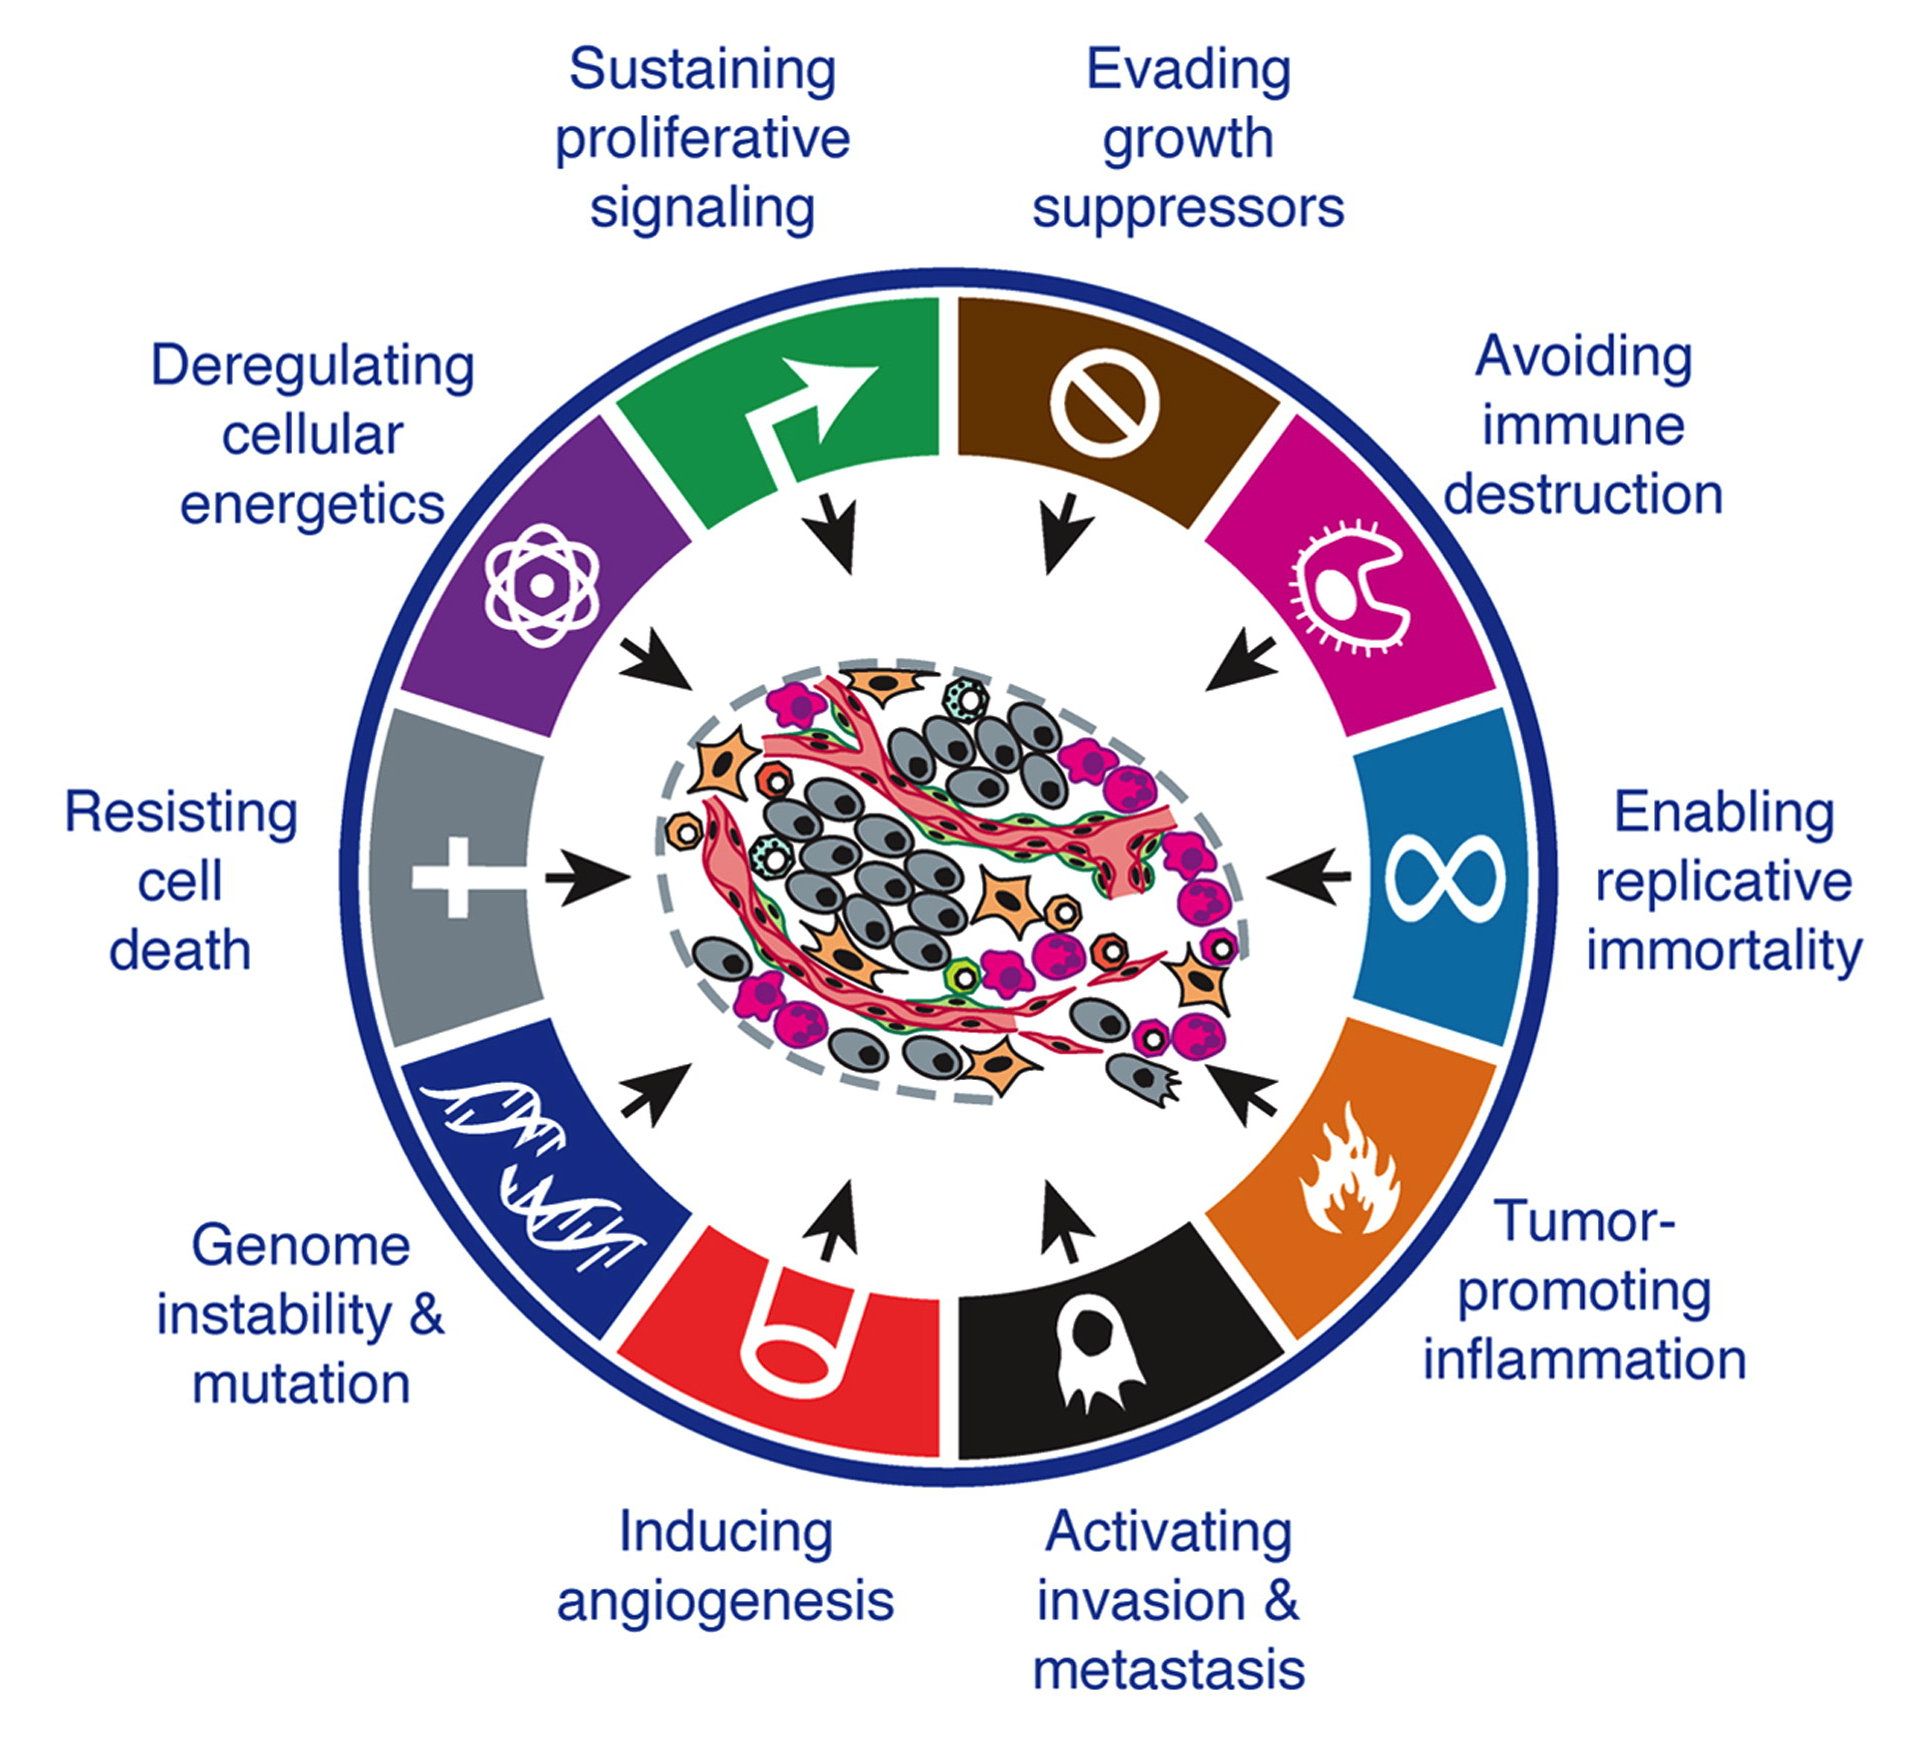
\includegraphics[width=0.9\linewidth]{fig/hallmarks} 

}

\caption[Hallmarks of cancer]{\textbf{Hallmarks of cancer.} The different
biological capabilities acquired by cancer cells, as described in
\citet{hanahan2000hallmarks}. Reprinted from
\citet{hanahan2011hallmarks}.}\label{fig:hallmarks}
\end{figure}






Each of these characteristics, or hallmarks, constitutes a research
program in its own right. And for each one there are genetic
alterations. These are tissue-specific or not, specific to a hallmark or
common to several of them \citep{hanahan2000hallmarks}. In any case,
\textbf{cancer can only result from the combination of different
alterations that invalidate several protective mechanisms} at the same
time. This is often part of a multi-step process of hallmark acquisition
that has been experimentally documented in some specific cases
\citep{hahn1999creation} or more recently inferred from genome-wide data
for human patients \citep{tomasetti2015only}. In summary, it appears
that in order to study the functioning of cancer cells it is necessary
to look at several mechanisms and to be able to consider them not
separately but together, in as many different patients as possible. This
ambitious programme has been made possible by a technological
revolution.

\section{The new era of genomics}\label{the-new-era-of-genomics}

\subsection{From sequencing to multi-omics
data}\label{from-sequencing-to-multi-omics-data}

In 2001, the first sequencing of the human genome symbolized the
beginning of a new era, that of what will become \textbf{high-throughput
genomics} \citep{lander2001initial, venter2001sequence}. From the end of
the 20th century, biological data started to accumulate at an
ever-increasing rate \citep{reuter2015high}, feeding and accelerating
cancer research in particular
\citep{stratton2009cancer, meyerson2010advances}. The ability to
sequence the human genome as a whole, for an ever-increasing number of
individuals, has enabled \textbf{less biased and more systematic studies
of the causes of cancer} \citep{lander2011initial}. The number of genes
associated with cancer increased drastically and some very important
genes such as BRAF of PIK3CA have been identified
\citep{davies2002mutations, samuels2004high}. Progress also extended to
the gene expression data. Gene-expression arrays have made an important
contribution by providing access to transcriptomic data (RNA), i.e.~what
has been transcribed from DNA and is therefore one step further in terms
of biological information. This information has made it possible to
further explore the differences betwween normal and tumor cells
\citep{perou1999distinctive}, or even to refine the classification of
cancers, which until now has been done mainly according to the tumor
site. Breast cancers are thus divided into subtypes with different
combinations of molecular markers that facilitate the understanding of
clinical behavior \citep{perou2000molecular}. One step further, we also
note the appearance of prognostic gene signatures such as gene
expression patterns correlated with the survival of patients
\citep{van2002gene}. This revolution was then extended to other types of
data such as proteins (proteomics), reversible modifications of DNA or
DNA-associated proteins (epigenomics), metabolites (metabolomics) and
others, each representing a perspective that can complement the others
to better understand biological mechanisms, particularly in the case of
diseases \citep{hasin2017multi}. We have thus entered the era of
multi-omics data \citep{vucic2012translating}.

\subsection{State-of-the art of cancer
data}\label{state-of-the-art-of-cancer-data}

With respect to cancer in particular, this wealth of data is
particularly represented by a family of \textbf{studies conducted by The
Cancer Genome Atlas (TCGA) consortium}, started in 2008
\citep{cancer2008comprehensive}. Cohorts of several hundred patients are
thus sequenced over the years for different types of cancer
\citep{cancer2012comprehensive}, resulting today in a total of 11,000
tumors from 33 of the most prevalent forms of cancer
\citep{ding2018perspective}. Figure \ref{fig:tcga} provides a partial
but striking overview of the depth of data available under this program.
We can see the frequencies of alterations of certain groups of genes for
a list of cancer types, making it possible to visualize the disparities
already anticipated in section \ref{epidemio} based on patient survival.
There are indeed important differences between the organs but also
between the different subtypes associated with the same organ. And this
representation only corresponds to one layer of data, that of genetic
alterations. It could be used for transcriptomic, epigenomic or
proteomic data, thus giving rise to an incredibly complex photography.

\begin{figure}

{\centering 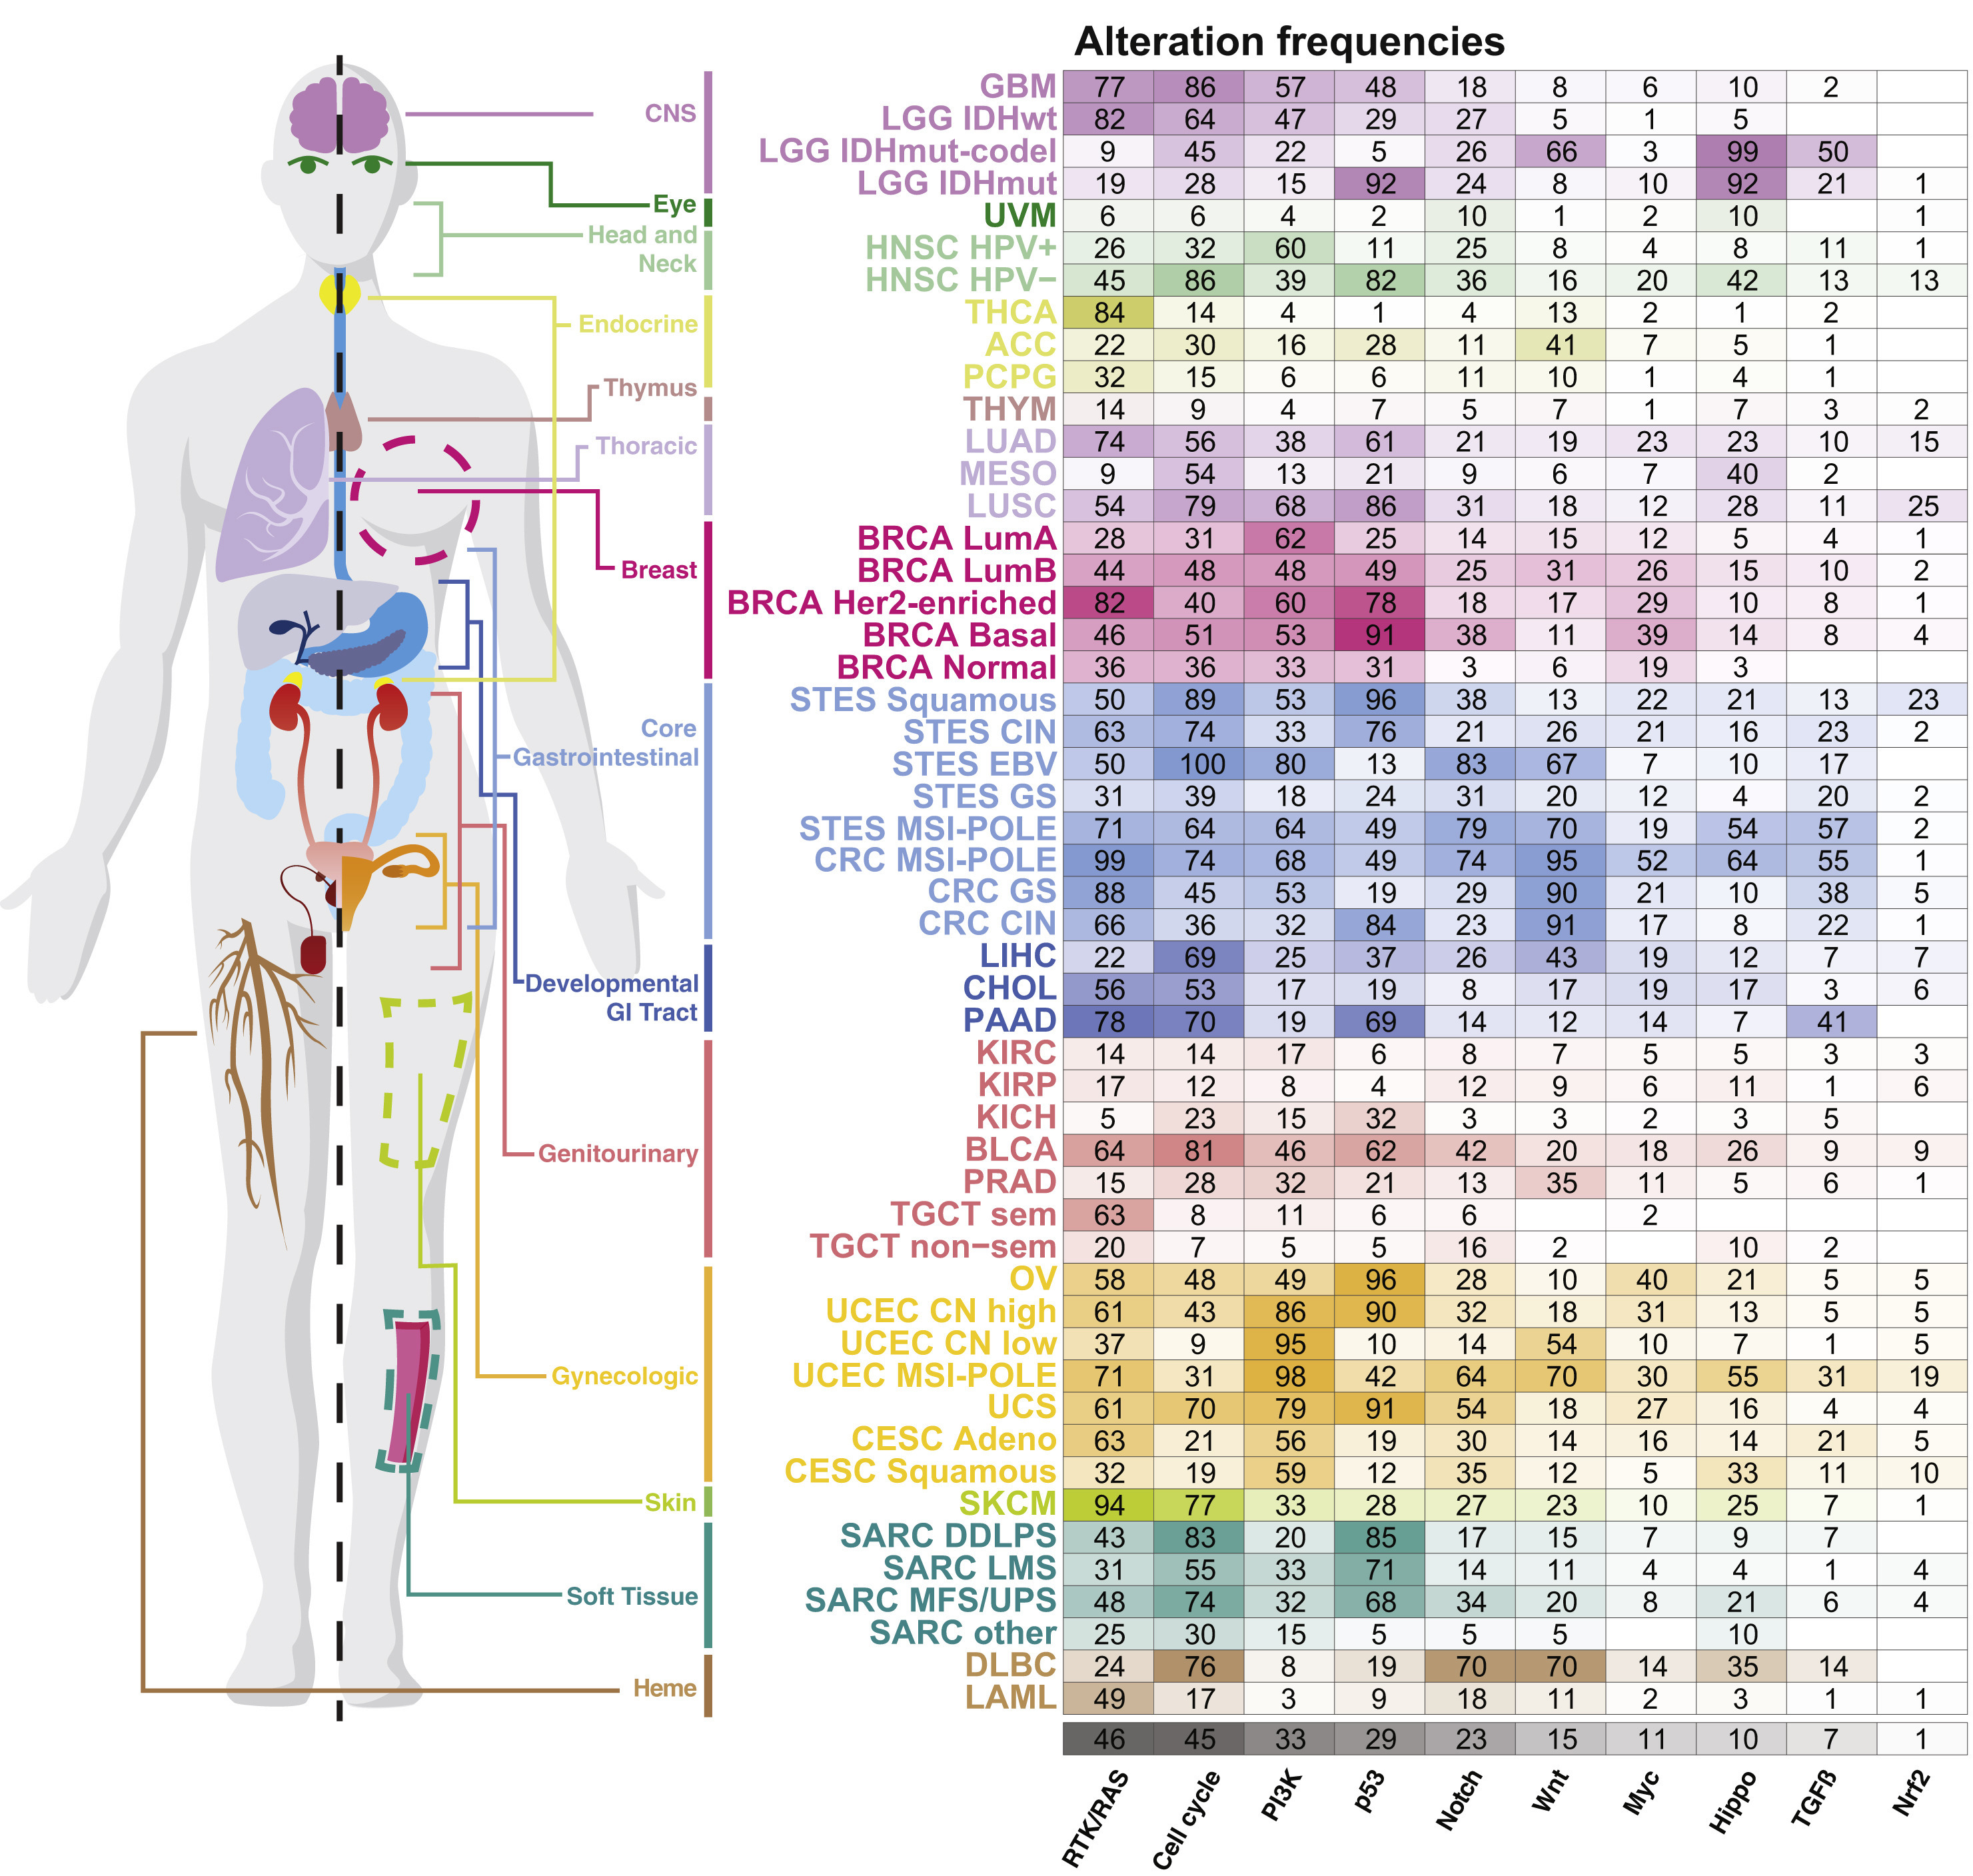
\includegraphics[width=0.9\linewidth]{fig/tcga} 

}

\caption[Genetic alterations frequencies for cancer types from TCGA data]{\textbf{Genetic alterations frequencies for cancer
types from TCGA data.} Frequencies of alteration per pahway and tumor
types as summaried in Pan-cancer analyses from TCGA data. Reprinted from
\citet{sanchez2018oncogenic}.}\label{fig:tcga}
\end{figure}






However, the diversity of data available for cancer research extends far
beyond this, both in terms of technology and type of data. This may be
data from model organisms such as mice or tumors of human origin made
more suitable for experimentation. In the latter category, it is crucial
to mention the \textbf{huge amount of data available on cell lines},
extracted from human tumors and transformed to be studied in culture. It
is then possible to go beyond descriptive data and vary the experimental
conditions in order to study the responses of these cells to
perturbations and to enrich our knowledge. This provides an opportunity
to know the response to more than 100 drugs of about 700 cell lines
\citep{yang2012genomics}. The richness of these data, coupled with the
omic profiling of each cell line, enables to study the determinants of
response to treatment with unprecedented scope
\citep{iorio2016landscape}. More recently, but following a similar
logic, other types of inhibition screenings have been proposed based on
a more specific technique called CRISPR-Cas9
\citep{behan2019prioritization}. The simplicity of the cell lines in
relation to the original tumors makes all these studies possible but
sometimes hinders the clinical application of the knowledge acquired.
For this reason, other types of biological models have been developed,
including patient-derived xenografts (PDX) which is an implant of human
tumors in mice to maintain the existence of a certain tumor
microenvironment \citep{hidalgo2014patient}, while maintaining drug
screening possibilities \citep{gao2015high}. These two types of data,
cell lines and PDX, have been used in this thesis, in addition to TCGA
patient data, thus justifying the limitation of this presentation, which
could otherwise be extended to other types of biological models.
Similarly, other technologies are becoming increasingly important in the
generation of cancer data, such as single-cell sequencing
\citep{navin2015first}, but will not be used in this work.

\section{Data and beyond: from genetic to network
disease}\label{data-and-beyond-from-genetic-to-network-disease}

All that remains to be done now is to make sense of all these data, to
organize it, because \textbf{cancer understanding does not flow directly
from the abundance of data}, and the ability to produce it may have been
outpaced by the ability to analyze it \citep{stadler2014cancer}. A
striking example is that of the prognostic signatures mentioned above.
The many signatures or lists of genes proposed, even for the same cancer
type, share relatively few genes, are difficult to interpret and their
efficiency is sometimes poorly reproducible \citep{domany2014using}.
Even more surprisingly, most signatures composed of randomly selected
genes were also found to be associated with patient survival
\citep{venet2011most}. One of the main avenues for improving the
interpretability of the data is the \textbf{integration of the prior
knowledge} we have of the phenomena, especially in the case of cancer
\citep{domany2014using}.

\begin{figure}

{\centering 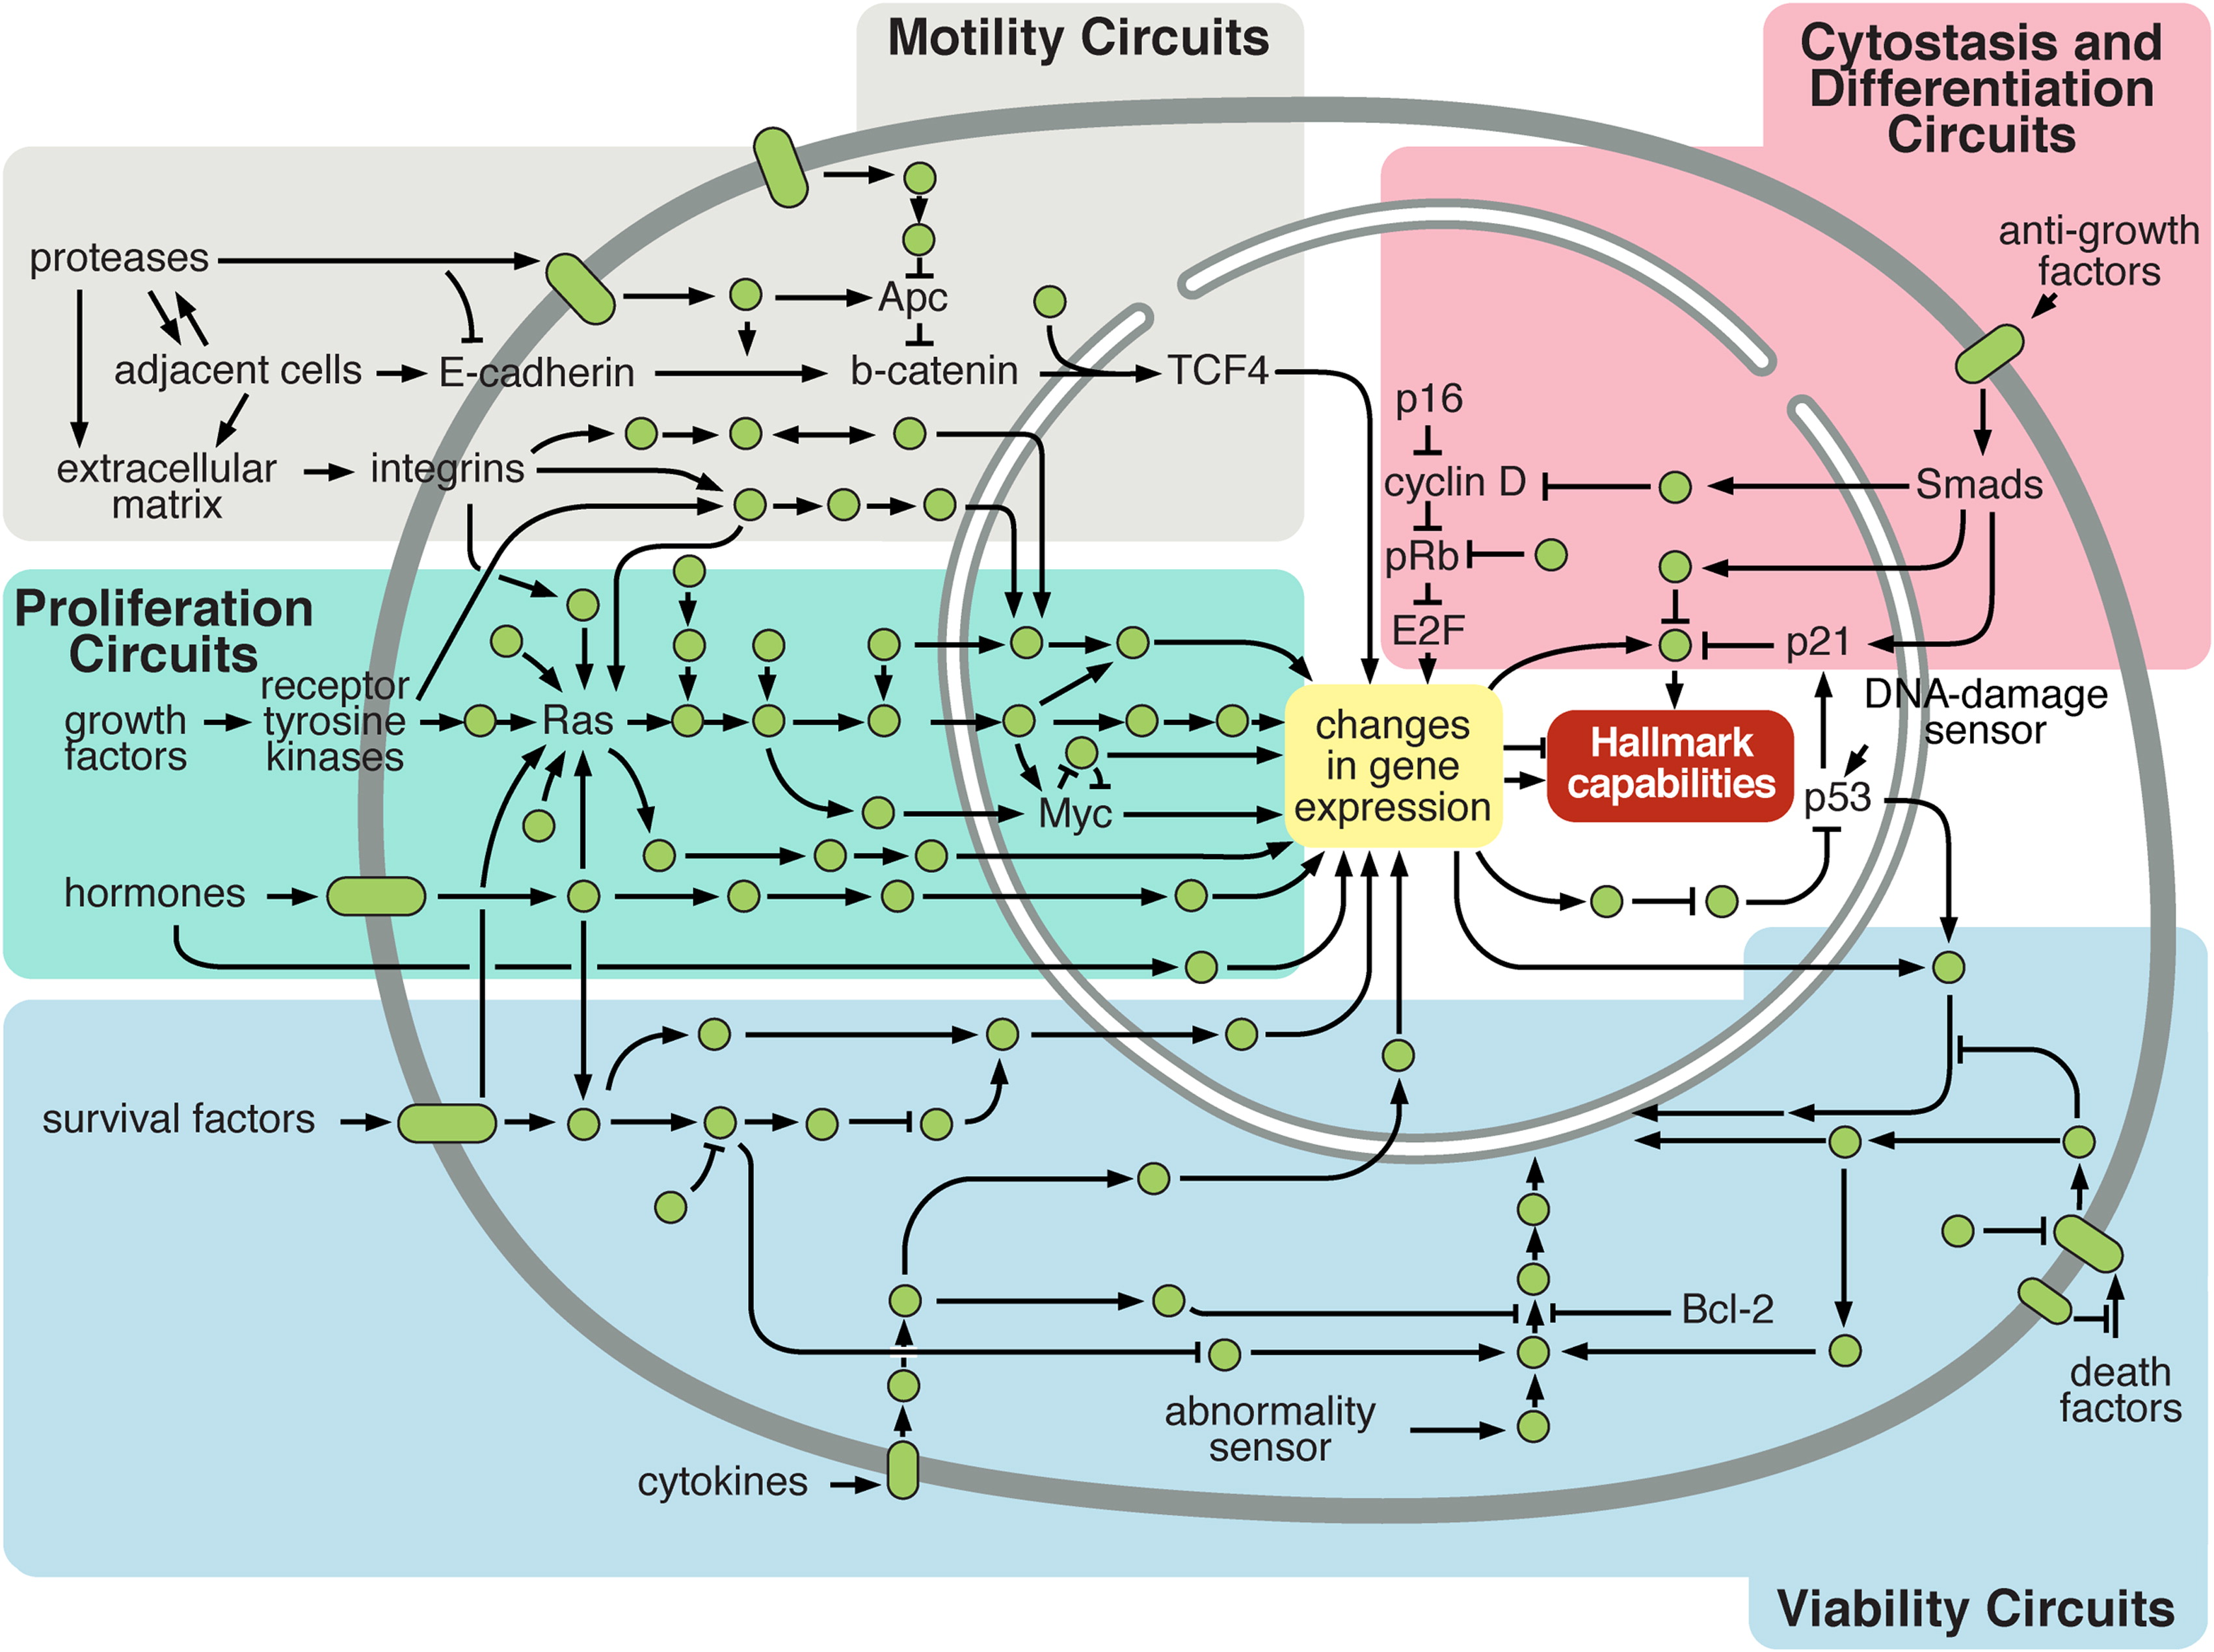
\includegraphics[width=0.9\linewidth]{fig/circuit} 

}

\caption[Simplistic representation of cellular circuit and pathways]{\textbf{Simplistic representation of cellular
circuitry.} Normal cellular circuit sand sub-circuits (identified by
colours) can be reprogrammed to regulate hallmark capabilities within
cancer cells. Reprinted from \citet{hanahan2011hallmarks}.}\label{fig:circuit}
\end{figure}






This \emph{a priori} knowledge is in fact already present in Figure
\ref{fig:tcga} since genetic alterations have been grouped in several
categories called pathways. A pathway is group of biological entities,
and associated chemical reactions, working together to control a
specific cell function like apoptosis or cell division. The interest of
these groupings may be understood based on the description of hallmarks.
Indeed, if the ``aim'' of a cancer cell is to inactivate each of the
protective functions, then it is more relevant to think not by gene but
by function. Inactivating only one of the genes associated with the
function may be sufficient and it is no longer necessary to inactivate
the others. Numerous alterations in a large number of genes in various
patients result often in the same key impaired pathways, like
alterations of cell cycle or angiogenesis for instance
\citep{jones2008core}. It is therefore possible to improve the stability
and interpretability of analyses by moving \textbf{from the gene scale
to the pathway scale} \citep{drier2013pathway}. More generally, the
integration of biological knowledge often leads to improved performance
in various cancer-related prediction tasks, either through the selection
of variables or by taking into account the structure of the variables
\citep{bilal2013improving, ferranti2017value}. Increasingly, the
biological variables are not interpreted separately but in relation to
each other \citep{barabasi2004network}. This is reflected in the
emergence of more and more resources to summarize and represent
signaling pathways and associated networks such as SIGNOR
\citep{perfetto2016signor}, OmniPath \citep{turei2016omnipath} or the
Atlas of Cancer Signaling Network \citep{kuperstein2015atlas}. Like
other diseases, cancer then goes \textbf{from a genetic disease to a
network disease} \citep{del2010diseases} and one can study how all kinds
of genetic alterations affect the wiring of these networks
\citep{pawson2007oncogenic}, and modify the cellular functions leading
to the previously described cancer hallmarks as depicted schmatically in
Figure \ref{fig:circuit}. In short, the richness of the data did not
make it less necessary to use prior knowledge in order to make the
analyses more interpretable and more robust.

\begin{figure}

{\centering 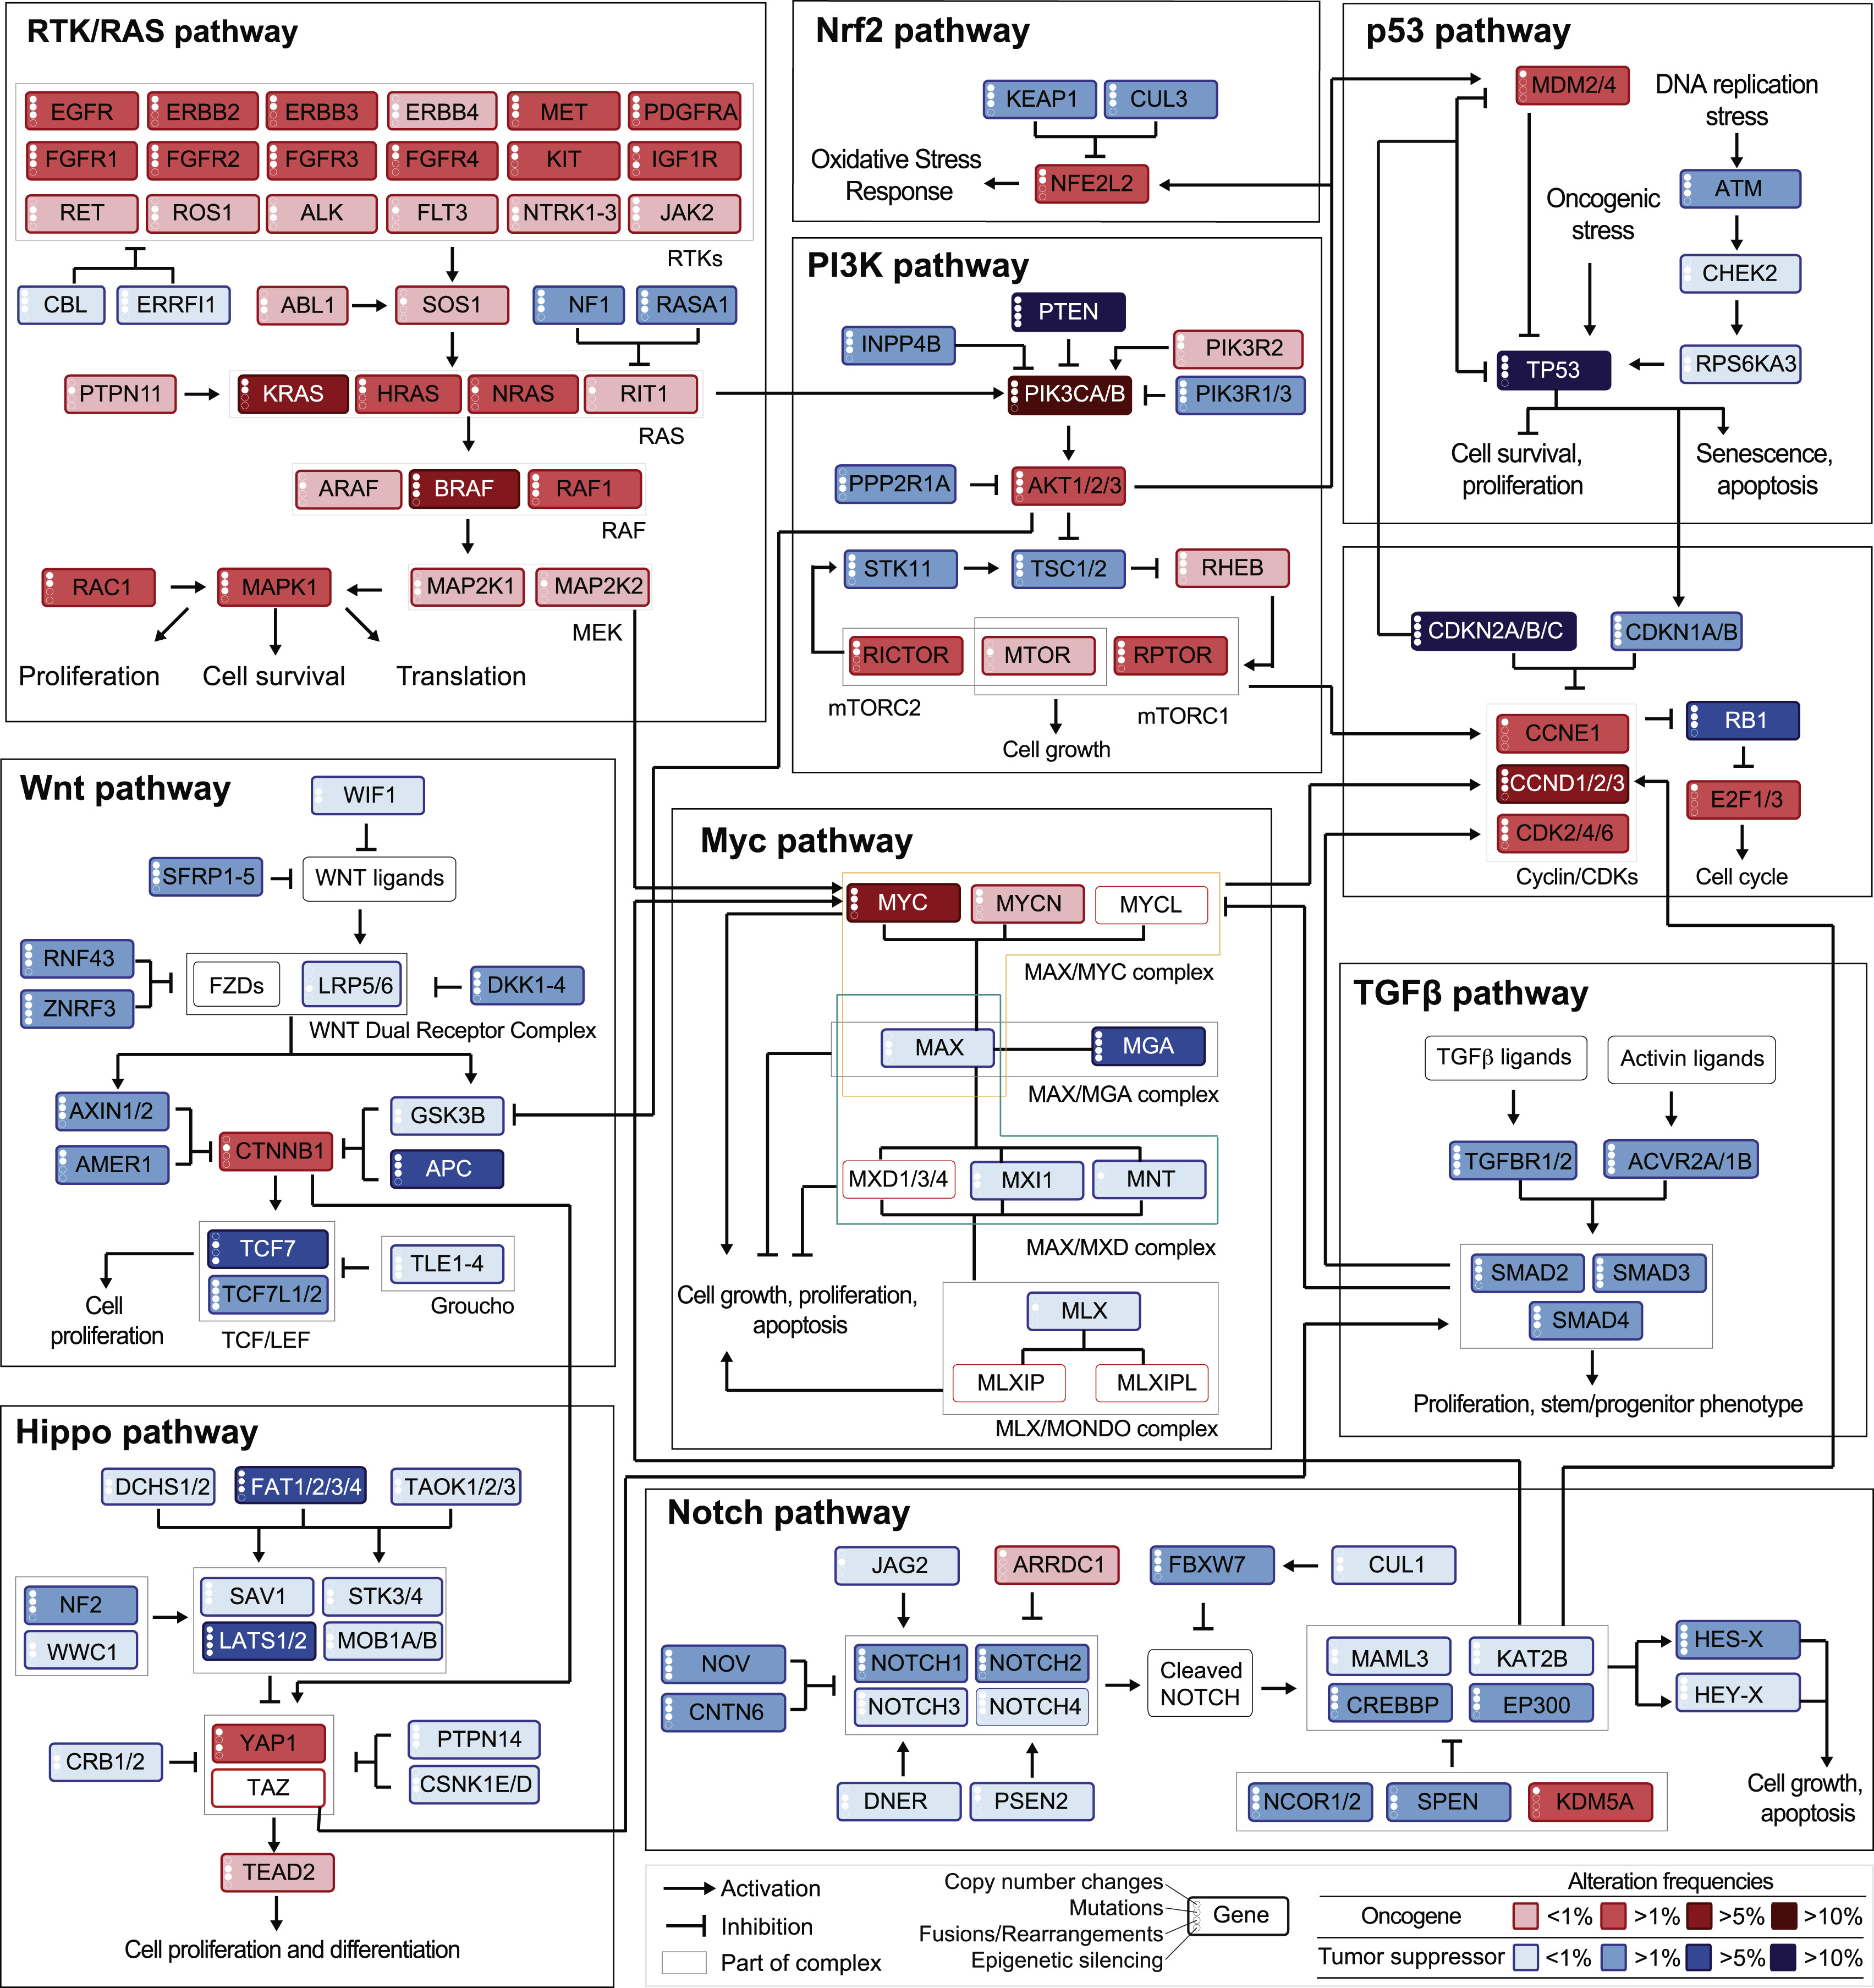
\includegraphics[width=0.9\linewidth]{fig/pathways} 

}

\caption[Genetic alterations frequencies from TCGA data mapped on a schematic signaling network]{\textbf{Genetic alterations frequencies from TCGA
data mapped on a schematic signaling network.} Frequencies of alteration
per pathway and tumor types as summarized in Pan-cancer analyses from
TCGA data. Reprinted from \citet{sanchez2018oncogenic}.}\label{fig:pathways}
\end{figure}






The final step, to obtain one of the most complete and integrated
visions of cancer biology, is then to integrate omics knowledge with
knowledge about the structure of pathways to try to understand in detail
how their combinations can lead to so many cancers that are both similar
and different. An example of such a representation is given by mapping
the TCGA data about genetic alterations, presented in Figure
\ref{fig:tcga}, on a representation of the different pathways showing
not only their internal organization but also their cross-talk
\citep{sanchez2018oncogenic}. This representation is proposed in Figure
\ref{fig:pathways} and is one the most recent and comprehensive view of
the kind of tools and data available to the modeller who wants to
dissect more deeply the mechanisms involved in cancer.

\chapter{Mechanistic modeling of cancer: from complex disease to systems
biology}\label{mechanistic-cancer}

\epigraph{"How remarkable is life? The answer is: very. Those of us who deal in networks of chemical reactions know of nothing like it... How could a chemical sludge become a rose, even with billions of years to try."}{George Whitesides}

\initial{T}he previous chapter identified the need to organize cancer
knowledge and data. The integration of biological knowledge,
particularly in the form of networks, is a first step in this direction.
The deepening of knowledge, however, requires the ability to manipulate
objects even more, to experiment, to dissect their behaviour in an
infinite number of situations, such as the astronomer with his orrery or
physicians with their old anatomical models (Figure \ref{fig:anatomy}).
Is it then possible to create mechanistic models of cancer in the same
way?

\begin{figure}

{\centering \includegraphics[width=0.9\linewidth]{fig/anatomy} 

}

\caption[Dissecting a biological phenomenon using a non-computational model]{\textbf{Dissecting a biological phenomenon using a
non-computational model.} Rembrandt, \emph{The Anatomy Lesson of Dr
Nicolaes Tulp}, 1634, oil on canvas, Mauritshuis museum, The Hague}\label{fig:anatomy}
\end{figure}





\section{Introducing the diversity of mechanistic models of
cancer}\label{introducing-the-diversity-of-mechanistic-models-of-cancer}

Modeling cancer is not a new idea. And the diversity of biological
phenomena involved in cancer has given rise to an equally important
diversity of models and formalisms, which we seek here to give a brief
overview in order to better identify the specific models that we will
focus on later. One way to order this diversity is to consider the
scales of these models (Figure \ref{fig:multiscale}). Indeed,
\textbf{cancer can be read at different levels, from the molecular level
of DNA and proteins, to the cellular level, to the level of tissues and
organisms} \citep{anderson2008integrative}. Models have been proposed at
all these scales, using different formalisms
\citep{bellomo2008foundations} and answering different questions.

Consistent with the evolution of knowledge and data, the early models
were at the \textbf{macroscopic level}. While methods and terminologies
may have changed, there are nevertheless traces of these models as early
as the 1950s. We then speak rather of mathematical modeling with a
meaning that is nevertheless intermediate between what we have defined
as mechanistic models and statistical models
\citep{byrne2010dissecting}. First, the initiation of tumorigenesis was
theorized with biologically-supported mathematical expressions in order
to make sense of cancer incidence statistics
\citep[\citet{knudson1971mutation}]{armitage1954age}. These models,
however, remained relatively descriptive in that they did not shed any
particular light on the biological mechanisms involved and focused on
gross characteristics of tumours. The integration of more advanced
knowledge as well as the progressive refinement of mathematical
formalisms has nevertheless allowed these models to proliferate while
gaining in interpretability, with for instance mechanistic models of
metastatic relapse \citep{nicolo2020machine}. Always on a macroscopic
scale, the study of tumor growth has also been the playground of many
mathematicians {[}\citet{araujo2004history}; byrne2010dissecting{]},
even predicting invasion or response to surgical treatments using
spatial modeling \citep{swanson2003virtual}. This line of research is
still quite active today and provides a mathematical basis for
comparison with tumour experimental growth
\citep{benzekry2014classical}.

\begin{figure}

{\centering 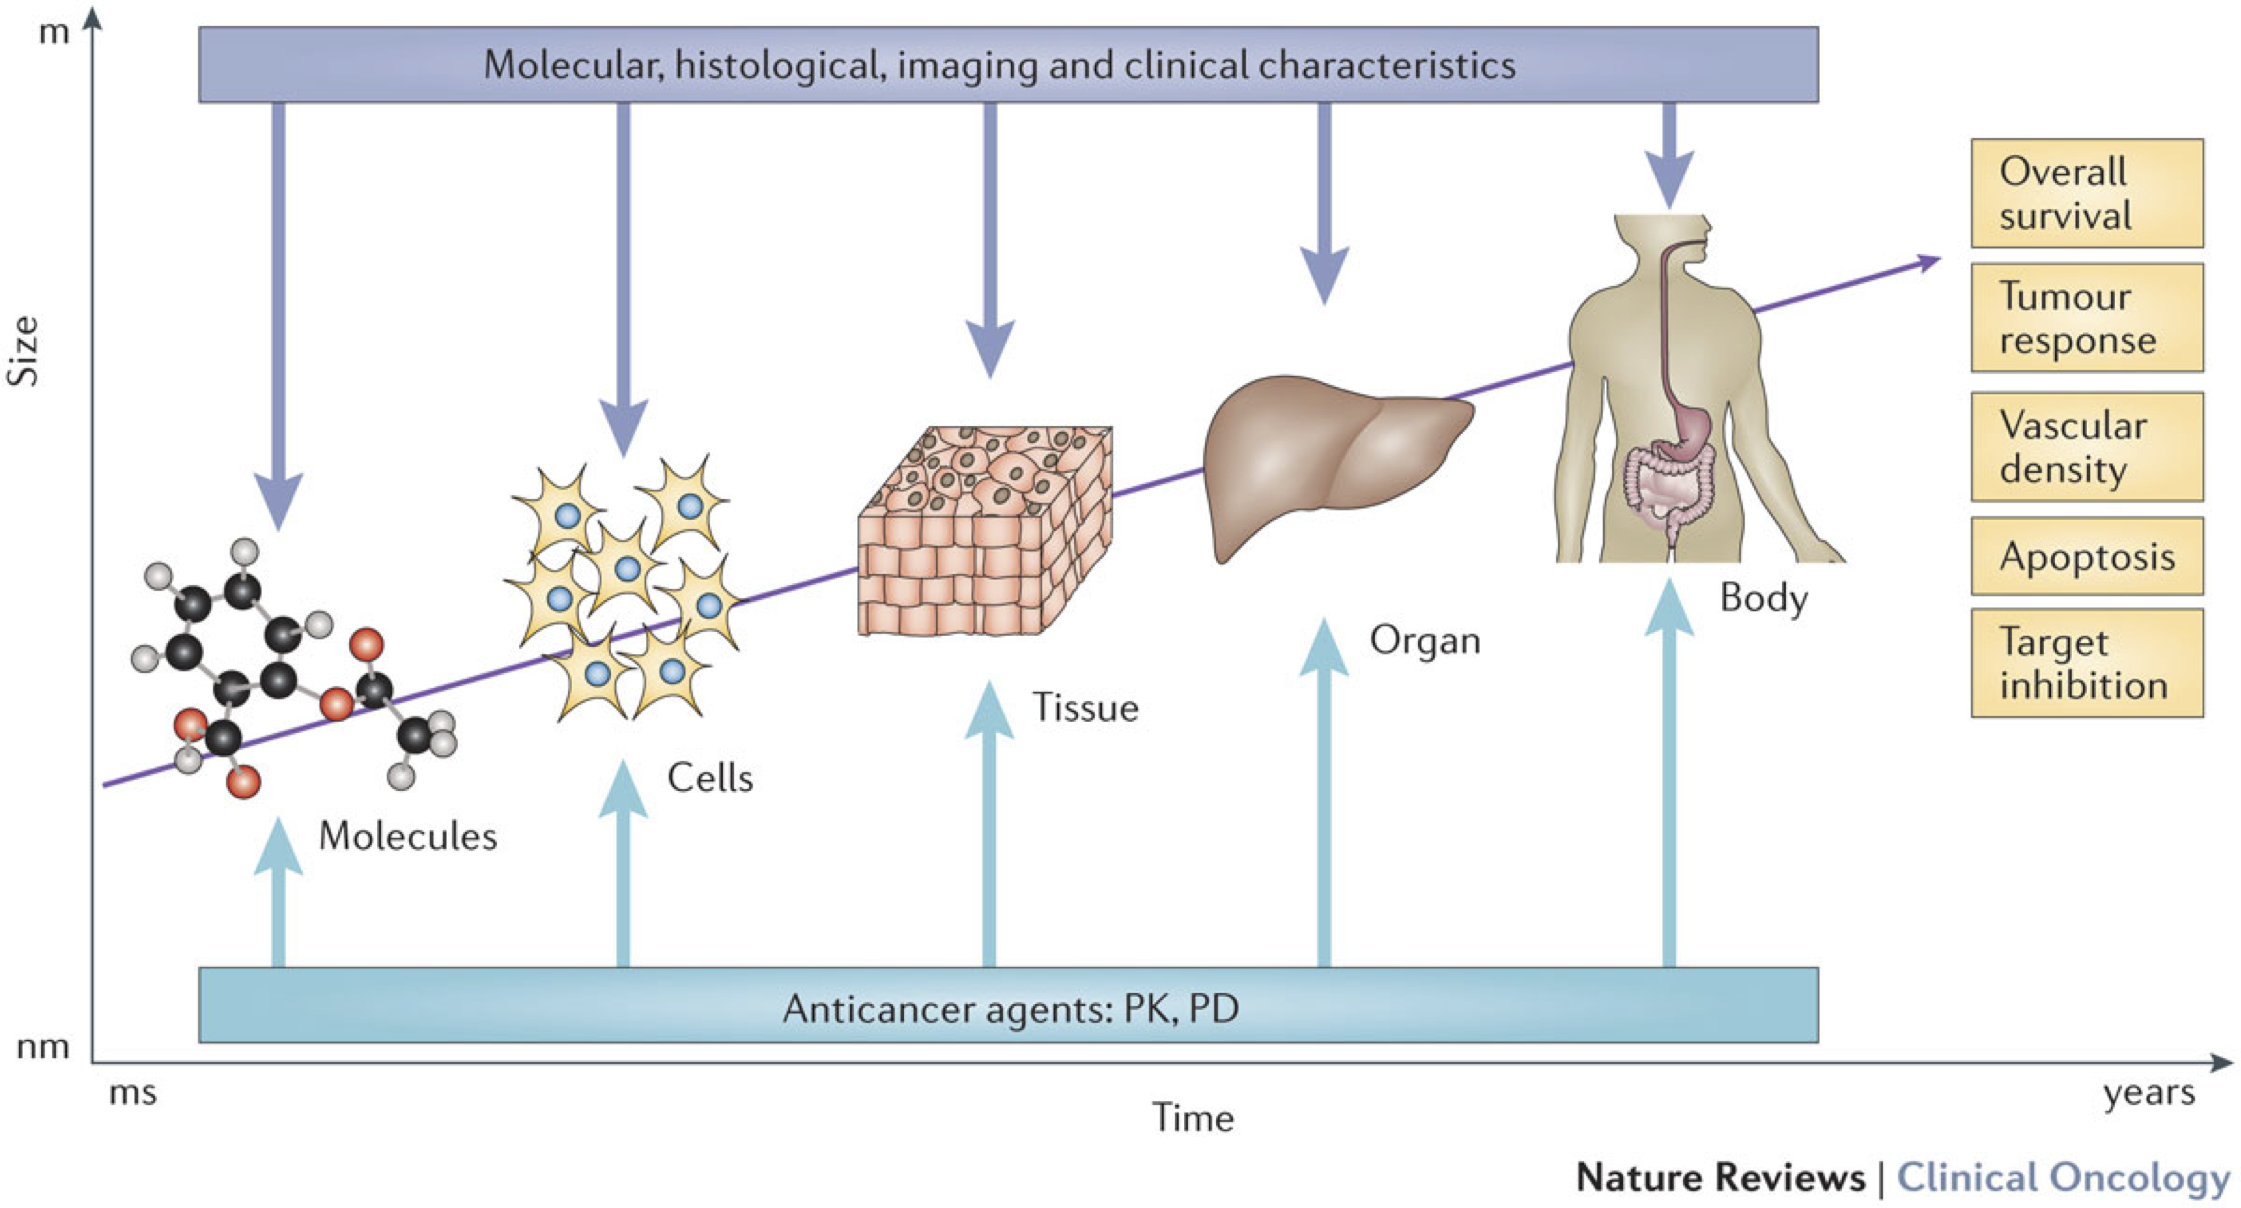
\includegraphics[width=0.9\linewidth]{fig/multiscale} 

}

\caption[The different scales of cancer modeling]{\textbf{The different scales of cancer
modeling.} Cancer can be approached at different scales, from molecules
to organs, using different data (dark blue), but often with the direct
or indirect objective of contributing to the study of clinically
interpretable phenomena (yellow boxes), in particular by studying the
influence of anticancer agents (pale blue). Reprinted from
\citet{barbolosi2016computational}.}\label{fig:multiscale}
\end{figure}









Taking it down a step further, it is also possible to model cancer at
the \textbf{cellular level}, for example by looking at the clonal
evolution of cancer \citep{altrock2015mathematics}. The aim is then to
understand the impact of the processes of mutation, selection, expansion
and cohabitation of different populatons of cells, at specifc rates. The
accumulation of a mutation in a population of cells can thus be studied
\citep{bozic2010accumulation}. Modeling at the cellular level is well
suited to the study of interactions between cells, between cancer cells
and their environment or with the immune system. Similar to other kinds
of studies of population dynamics, formalisms based on differential
equations are quite common \citep{bellomo2008foundations}; but there are
many other methods such partial differential equations or agent-based
modeling \citep{letort2019physiboss}.

Finally, at an even smaller scale, it is possible to model the
\textbf{molecular networks} at work in cells \citep{le2015quantitative}.
The aim is then to simulate mathematically how the different genes and
molecules regulate each other, transmit information and, in the case of
cancer, end up being deregulated \citep{calzone2010mathematical}. These
models will be the subject of the thesis and will therefore be defined
more precisely and used to detail the concepts and tools of systems
biology in the following sections. It can already be noted that while
these models can integrate the most fundamental biological mechanisms of
living organisms, one of the most burning questions is whether it is
possible to link them to the larger scales that are clinically more
interesting (tissues, organs etc.). Can these models tell us something
about the molecular nature of cancer? About patient survival? Their
response to treatment? These questions apply to all of the above models,
whatever their scales (Figure \ref{fig:multiscale}), but are more
difficult to answer for models defined at molecular scale that are
further from the clinical data of interest. The aim of this thesis is to
provide potential answers to these questions. One of the ways of
approaching these issues has been to propose multi-scale models, which
are nevertheless very complex
\citep{anderson2008integrative, powathil2015systems}. We will focus here
on the use of models defined almost exclusively at the molecular scale,
which is assumed to be prominent, to study what can be inferred on the
larger scales.

\section{Cell circuitry and the need for cancer systems
biology}\label{cell-circuitry-and-the-need-for-cancer-systems-biology}

Most biological systems, and certainly cells, fall into the category of
\textbf{complex systems}. These are systems made up of many interacting
elements. While these systems can be found in many different scientific
fields, the cell as a complex system is characterized by the diversity
and multifunctionality of its constituent elements (genes, proteins,
small molecules, enzymes), which nevertheless contribute to organized
and a priori non-chaotic behaviour \citep{kitano2002computational}.
Thus, the role of a protein such as the p53 tumour suppressor can only
be understood by taking into account the interplay between its
relationships with transcription factors and biochemical modifications
of the molecule itself \citep{kitano2002computational}. In a cell, as in
any complex system, the multiplication of components and interactions
can make the response or behaviour of the system unexpected or
unpredictable. Non-linear responses, such as abrupt changes in the state
of a system, called critical transitions, can be observed in response to
a moderate change in the signal \citep{trefois2015critical}. Generally
speaking, it is possible to observe \textbf{emergent behaviours},
i.e.~behaviours of the system as a whole that were not trivially
deducible from the individual behaviours of its components. This has
been documented, through experiments and simulations, in the study of
cell signalling pathways and the resulting biological decisions
\citep{bhalla1999emergent, helikar2008emergent}. These considerations
have thus given rise to \textbf{system-level or holistic approaches that
aim to integrate data and knowledge into more comprehensive
representations, often called systems biology}.

What is true for the cell in general is just as true for cancer in
particular. Understanding the intertwining of signaling pathways is
necessary to study their contributions to different cancer hallmarks, as
shown in Figure \ref{fig:circuit}. The concepts described above can thus
be transposed to \textbf{cancer systems biology}
\citep{hornberg2006cancer, kreeger2010cancer, barillot2012computational}.
Indeed, it is often a question of understanding or predicting the impact
of perturbations on cellular networks. Understanding how a single
genetic mutation disrupts and reprograms networks, or even predicting
the responses triggered by a drug on a presumably promising molecular
target, makes little sense without integrated approaches. In addition,
cancers are characterized by the accumulation of numerous mutations and
alterations over time that must be considered concomitantly. These
points of view of biologists and modellers reinforce the observation
already made in the previous chapter of cancer as a network disease, as
a system disease (Figure \ref{fig:pathways}).

Finally, to conclude this general presentation, it is important to
understand that while small molecular network modeling is not recent,
the rise and multiplication of wide range systems biology approaches is
very much related to the production of biological data
\citep{de2002modeling}. The last few decades have seen the emergence of
high-throughput data that have made it possible to identify and link
hundreds of genes or proteins involved in cancer. Exploring the
interaction and back and forth between these models and the data they
use or predict is therefore of utmost importance. In addition, the now
** massive amount of data has also imposed mathematical or computational
approaches as a central element in the management of this profusion**
and more and more modeling approaches are focused on data integration or
inference \citep{frohlich2018efficient, bouhaddou2018mechanistic}. More
generally, Figure \ref{fig:pubmed} shows that while the number of
scientific articles devoted to cancer has increased drastically since
the 1950s (panel A), the proportion of these same articles mentioning
\emph{models}, \emph{networks} or \emph{computational} approaches has
also increased (panel B), illustrating a change in paradigms.

\begin{figure}

{\centering 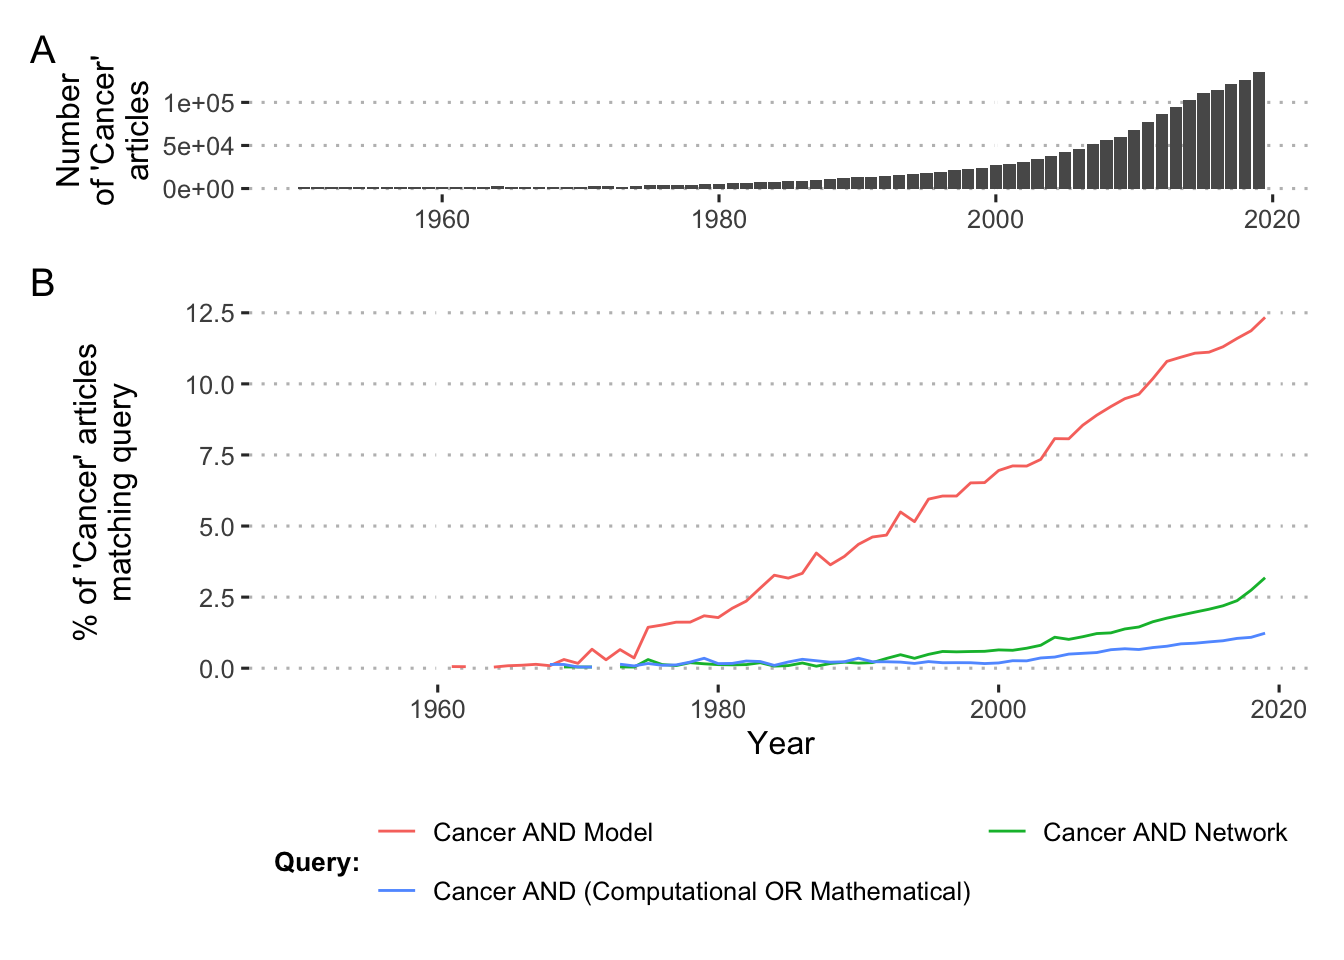
\includegraphics[width=0.9\linewidth]{03-Mechanistic_files/figure-latex/pubmed-1} 

}

\caption[PubMed trends in cancer studies.]{\textbf{PubMed trends in cancer studies.} (A)
PubMed articles with the word \emph{Cancer} in either title or abstract
from 1950 to 2019. (B) Proportion of the \emph{Cancer} articles with
additional keywords expressed as PubMed logical queries.}\label{fig:pubmed}
\end{figure}






\section{Mechanistic models of molecular
signaling}\label{mechanistic-models-of-molecular-signaling}

Once the context has been defined, both biologically and
methodologically, it is possible to begin the exploration of the models
that will constitute the core of this thesis: the \textbf{mechanistic
models of molecular networks} and signaling pathways. Before describing
and illustrating some of the existing mathematical formalisms, it is
possible to describe the common fundamental elements of this family of
approaches.

\subsection{Networks and data}\label{networks-and-data}

The first step is to identify the relevant biological entities from a
question or system of interest (e.g.~tumor suppressor genes, signaling
cascades of proteins) and then to model their interactions, the
regulatory relationships that link them. At this stage the model can
generally be represented by a network but this word can cover different
realities \citep{le2015quantitative}. The simplest network just
represents undirected interactions between entities, which therefore
only establishes relationships and not causal mechanisms. But modeling
requires more precise definitions, in particular concerning the
direction of the interaction (is it A that acts on B or the opposite)
and its nature (type of chemical reaction, activation/inhibition etc.).
This is usually summarized as \textbf{activity flows (or influence
diagrams) with activation and inhibition arrows} as in Figure
\ref{fig:circuit} or Figure \ref{fig:toyraf}A. These arrows emphasize
the transormation of static networks into dynamic objects that can be
manipulated and interpreted mechanistically. This work can be taken
further by writing bipartite graphs, known as process descriptions,
which explicitly show the different states of each variable (first type
of nodes), depending on their phosphorylation sate for instance, and the
reactions that link them (second type of nodes) as in Figure
\ref{fig:toyraf}B. A more precise description of these different
representations and their meanings can be found in
\citet{le2015quantitative}. \textbf{Once the network structure of the
model has been defined, it is possible write the corresponding
mathematical formalism} and potentially to refine certain parameters.
Finally, the model is often confronted with new data to check its
consistency with the biological behaviour studied or possibly make new
predictions.

However, all these steps are not linear and sequential, but rather
iterative and cyclical. This \textbf{modeling cycle}, with back and
forth to the data, is not specific to molecular network models, but it
is possible to specify it in this case (Figure \ref{fig:cycle}). The
names of the key players involved in the question of interest are thus
first extracted from adapted data or from the literature. A first
mathematical translation of the relationships between the entities is
then proposed before verifying the compatibility of this model with the
observations, whether qualitative or quantitative. If the compatibility
is not good, we come back to the definition or the parameterization of
the model. If compatibility is correct, the model can be used to make
new predictions or study phenomena that go beyond the initial data set.
Ideally, these predictions will be tested afterwards. This cyclic
approach with two successive checks is analogous to the use of
validation and test data in the evaluation of most learning algorithms.
This analogy can sometimes be masked by the qualitative nature of the
predictions or by the lack of explicit fitting of the parameters.

\begin{figure}

{\centering 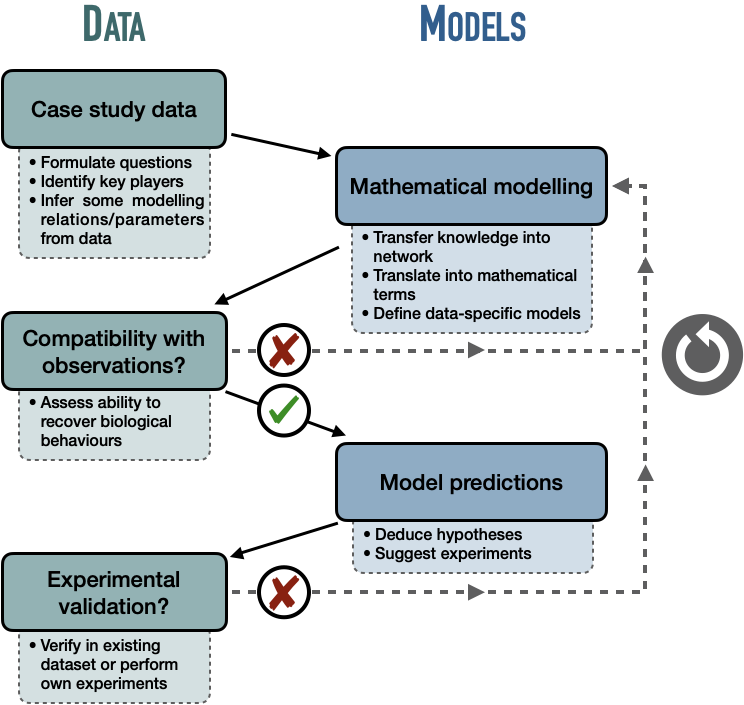
\includegraphics[width=0.7\linewidth]{fig/cycle} 

}

\caption[Modeling a biological network: an iterative and cyclical process]{\textbf{Modeling a biological network: an iterative
and cyclical process.} Reprinted from \citep{beal2020modelisation}. A
different and simpler version of this cycle is described in
\citep{le2015quantitative}.}\label{fig:cycle}
\end{figure}






\subsection{Different formalisms for different
applications}\label{different-formalisms-for-different-applications}

Beyond these similarities in the construction and representation of
models, the precise mathematical formalism that underlies them varies
according to the type of question and the data \citep{de2002modeling}.
For the sake of simplicity, and without exhaustiveness, we propose to
divide into quantitative and qualitative formalisms which will be
essentially illustrated respectively by \textbf{ordinary differential
equation (ODE)} models and \textbf{logical (or Boolean) models} for
which a graphical and schematic comparison is proposed in Figure
\ref{fig:toyraf}.

\begin{figure}

{\centering 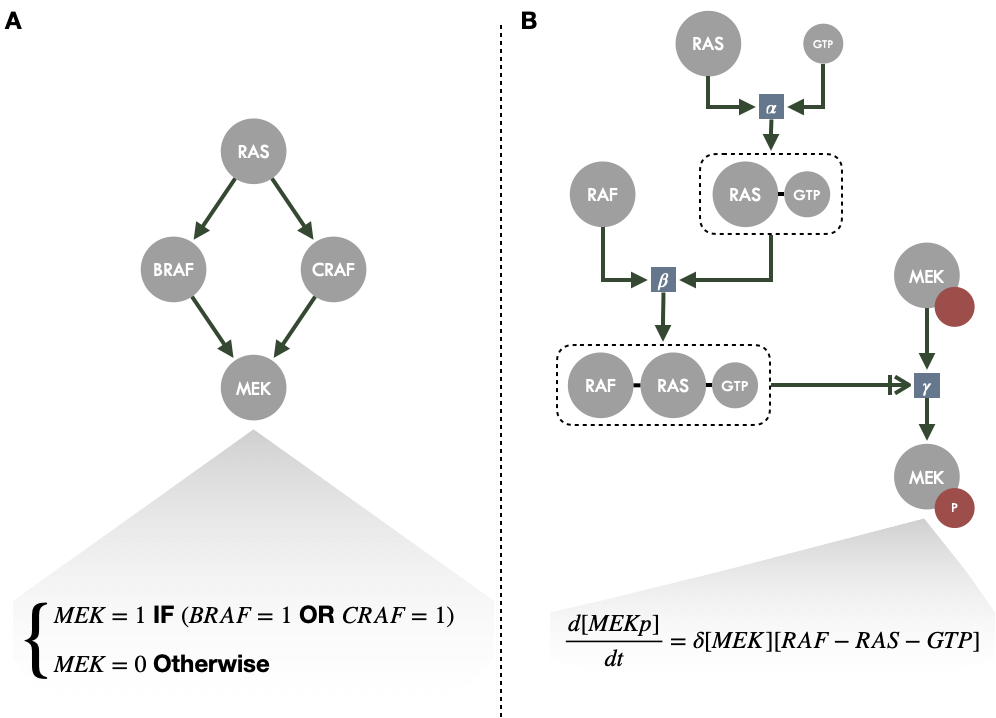
\includegraphics[width=0.9\linewidth]{fig/toyraf} 

}

\caption[Schematic example of logical and ODE modeling around MAPK signaling]{\textbf{Schematic example of logical and ODE
modeling around MAPK signaling.} (A) Activity flow diagram of a small
part of MAPK signaling, each node representing a gene or protein, with
an example of logical rule for MEK node for the corresponding logical
model. (B) Process description of the same diagram with BRAF and CRAF
merged in RAF for the sake of simplicity; each square representing a
reaction and the correspondong rate; an example differential equation is
provided for the phosphorylated (active) form of MEK.}\label{fig:toyraf}
\end{figure}










One of the most frequent approaches is the use of \textbf{chemical
kinetics} equations to construct ODE systems which are a fairly natural
translation of the process descritption networks described in the
previous section \citep{polynikis2009comparing}. Each biological
interaction is treated as a reaction governed by the law of mass action
and, under certain hypotheses, as a differential equation (Figure
\ref{fig:toyraf}B); the set of reactions in the system then generates a
set of differential equations with coupled variables, in an analogous
way to the Lotka Volterra system presented in section
\ref{lotkasection}. Thus the variables generally represent quantities of
molecular species, for example concentrations of RNA or proteins, and
the stoichiometric coefficients and reaction rates are used to define
the system parameters. Approximations are sometimes made to simplify the
equations, for example by assuming that they can be written as
Michaelis-Menten's enzymatic reactions, which have a simple and well
known behaviour. However, the theoretical accuracy of quantitative
models has a cost since \textbf{each differential equation requires
parameters}, such as reaction constants or initial conditions, to which
the system is very sensitive \citep{le2015quantitative}. The biochemical
interpretation of the parameters sometimes allow to find their value in
the literature, if the reactions are well characterized, even if
possible variations in a given biological or physical context are often
unknown. Since knowledge of the values of these parameters is often
limited or even non-existent, it may require a very large volume of data
(including time series) to fit the many missing parameters which can be
difficult if the number of parameters is large
\citep{villaverde2014reverse}. However, recent work has demonstrated the
feasibility and scalability of this type of inference with sufficiently
rich data \citep{frohlich2018efficient}.

At the same time, more qualitative approaches to modeling biological
networks have been proposed with discrete variables linked together by
rules expressed as logical statements \citep{abou2016logical}. These
models are both more abstract since variables do not have a direct
biological interpretation (e.g.~concentration of a species) but are more
versatile since they can unify different biological realities under the
same formalism (e.g.~activation of a gene or phosphorlation of a
protein). The discrete nature of the variables can then be seen as an
asymptotic case of the sigmoidal (e.g.~Hill function) relationships
often found in biology \citep{le2015quantitative}. The step function
thus obtained can keep a natural interpretation in the context of
biological phenomena: genes activated or not, protein present or absent
etc. Similarly, interactions between species are not quantified but are
based on a qualitative statements (e.g.~A will be active if B and C are
active), drastically reducing the number of parameters (Figure
\ref{fig:toyraf}A). If the theoretical interest of this formalism to
study biological mechanisms was proposed quite early
\citep{kauffman1969homeostasis, thomas1973boolean}, many concrete
applications have also been developed over the years, particularly in
cancer research \citep{saez2011comparing, remy2015modeling}. This
\textbf{logical formalism will constitute the core of the work presented
in Part II}, where it will therefore be discussed in greater detail.

\begin{table}

\caption{\label{tab:odelogic}\textbf{Features of quantitative and qualitative
modeling applied to biological molecular networks} (adapted from
\citet{le2015quantitative})}
\centering
\begin{tabular}[t]{>{\bfseries\raggedright\arraybackslash}p{6em}||>{\raggedright\arraybackslash}p{12em}|>{\raggedright\arraybackslash}p{12em}}
\hline
\rowcolor[HTML]{808080}  \multicolumn{1}{c}{\textcolor{white}{\textbf{ }}} & \multicolumn{1}{c}{\textcolor{white}{\textbf{Quantitative modeling}}} & \multicolumn{1}{c}{\textcolor{white}{\textbf{Qualitative modeling}}}\\
\hline
Example formalism & Ordinary differential equation (ODE) models & Logical models\\
\hline
Type of variables & Direct translation of biological quantities, usually continuous & Abstract representation of activity levels, usually discrete\\
\hline
Objective & Quantitatively accurate and temporal simulation of an experimental phenomenon & Coarse-grained simulation of qualitative phenotypes\\
\hline
Advantages & Direct confrontation with experimental data; precise; linear representation of time & Faster design; easy translation of literature-based assertions; simulation of perturbations\\
\hline
Drawbacks & Difficulty determining or fitting parameters & More difficult to link to data; lower precision\\
\hline
\end{tabular}
\end{table}





These two formalisms, which are among the most frequent for modelling
biological networks, share many similarities, in particular the
propensity to be built according to bottom-up strategies based on
knowledge of the elementary parts of the model, i.e.~biological entities
and reactions. However, they differ in their implementation and
objectives, \textbf{one aiming at the most accurate representation
possible, the other seeking to capture the essence of the system's
dynamics in a parsimonious way} (Table \ref{tab:odelogic}). The
opposition is not irrevocable, as illustrated by the numerous hybrid
formalisms that lie within the spectrum delimited by these two extremes
such as fuzzy logic or discrete-time differential equations
\citep{le2015quantitative, calzone2018logical}. To conclude, a
comparison between the two approaches applied to the same problem is
proposed by \citet{calzone2018logical}, studying the
epithelio-mesenchymal transition (EMT, a biological process involved in
cancer), to illustrate in concrete terms their complementarity.

\subsection{Some examples of complex
features}\label{some-examples-of-complex-features}

With the help of these models, both qualitative and quantitative, many
complex behaviours have been identified. Benefiting from the knowledge
accumulated in the study of dynamic systems, a whole zoo of patterns
with complex and non-intuitive behaviours such as non-linearities have
been highlighted \citep{tyson2003sniffers}. The MAPK pathway, coarsely
described in Figure \ref{fig:toyraf}, and often simplified as a rather
unidirectional cascade, shows switch or bistability behaviors generated
by the complexity of its multiple phosphorylation sites
\citep{markevich2004signaling}. These models have also been put at the
service of understanding cancer and the erroneous decision-making by
cells resulting from impaired signaling pathways. Thus,
\citet{tyson2011dynamic} summarize superbly well the complexity that can
be hidden in the dynamics of smallest molecular networks as soon as they
contain more than two entites and crossed regulations or feedback loops.
Logical models have also made it possible to better dissect some complex
phenomena at play in the cell such as emergent behaviours
\citep{helikar2008emergent} or mechanisms behind mutation patterns in
cancer \citep{remy2015modeling}.

\section{From mechanistic models to clinical
impact?}\label{from-mechanistic-models-to-clinical-impact}

Mechanistic models have therefore undeniably led to a better
understanding of the complex molecular machinery of signalling pathways.
But beyond the interest that this understanding represents, do these
models also have a clinical utility? In other words, \textbf{are they of
clinical or only scientific value?}

\subsection{A new class of biomarkers}\label{a-new-class-of-biomarkers}

Throughout this thesis, the clinical value of mechanical models will
often be analyzed by analogy to that of biomarkers. Throughout this
thesis, the clinical value of mechanical models will often be analyzed
by analogy to that of biomarkers. Biomarkers are usually defined as
measurable indicators of patient status or disease progression, such as
prostate-specific antigen (PSA) for prostate cancer screening or BRCA1
mutation for breast cancer risk \citep{henry2012cancer}. Biomarkers also
encompass multivariate signatures that identify more complex patterns
with clinical significance. Taking the logic even further, it was
therefore proposed that mechanistic models, which also reveal complex
molecular behaviours, could be considered as biomarkers, capturing
perhaps even dynamic information \citep{fey2015signaling}.

Like oncology biomarkers, the models will be divided into two categories
according to their clinical objectives: \textbf{prognostic models and
predictive models} \citep{oldenhuis2008prognostic}. Prognostic
biomarkers and models are those that provide information on the
evolution of cancer independently of treatment. They are therefore
generally confronted with survival or relapse data. The protein Ki-67
for example, encoded by the MKI67 gene, is known to be indicative of the
level of proliferation and high levels of expression are thus associated
with a poorer prognosis in many cancers \citep{sawyers2008cancer}.
Predictive biomarkers and models, on the other hand, give an indication
of the effect of a therapeutic strategy. The simplest example, but not
the only one, concerns biomarkers that are themselves the target of
treatment: treatments based on monoclonal antibodies directed against
HER2 receptors in breast cancer are only effective if the HER2 receptor
has been detected in the patient \citep{sawyers2008cancer}. Without
attempting to be exhaustive, some logical and ODE models, with either
prognostic or predictive claims, will be described.

\subsection{Prognostic models}\label{prognostic-models}

One of the first mechanical models of cell signalling to have been
explicitly presented as a prognostic biomarker is the one proposed by
\citet{fey2015signaling} and describing c-Jun N-terminal kinase (JNK)
pathway in neuroblastoma cells. A summary of the study is provided in
Figure \ref{fig:fey}). The model is an ODE translation of the process
description network of Figure \ref{fig:fey})A, further determined and
calibrated with molecular biology experimental data obtained using
neuroblastoma cell lines. We thus observe the non-linear switch-like
dynamics of JNK activation as a function of cellular stress (Figure
\ref{fig:fey})B). The precise characteristics of this sgmoidal response
can, however, vary from one individual to another as captured by the
network output descriptors \(A\), \(K_{50}\) and \(H\). Fey et al.
proposed to perform neuroblastoma patient--specific simulations of the
model, using patient gene expressions for ZAK, MKK4, MKK7, JNK and AKT
genes to specify the initial conditions of the ODE system. Since JNK
activation induces cell death through apoptosis, the patient-specific
\(A\), \(K_{50}\) and \(H\) derived from patient-specifc models are then
analyzed as prognostic biomarkers (Figure \ref{fig:fey})C). Readers are
invited to refer to the original article for details on model
calibration or binarization of network descriptors
\citep{fey2015signaling}. The authors also showed that in the absence of
positive feedback from \(JNK^{**}\) to \(^PMKK7\), an important
component of non-linearity, the prognostic value is drastically
decreased. All in all, this pipeline from ODE model to survival curves,
thus provides a \textbf{paradigmatic example of the clinical
interpretation of mechanistic models of molecular networks} that will be
reused in later chapters for illustration purposes. Other ODE models
following a similar rationale have been proposed by the same group for
colorectal cancer \citep{hector2012clinical, salvucci2017stepwise} or
glioblastoma {[}\citet{murphy2013activation}; salvucci2019system{]}.
Machine learning approaches have also been proposed to ease the clinical
implementation of this kind of prognostic models by dealing with the
potential lack of patient data needed to personalize them
\citep{salvucci2019machine}.

\begin{figure}

{\centering 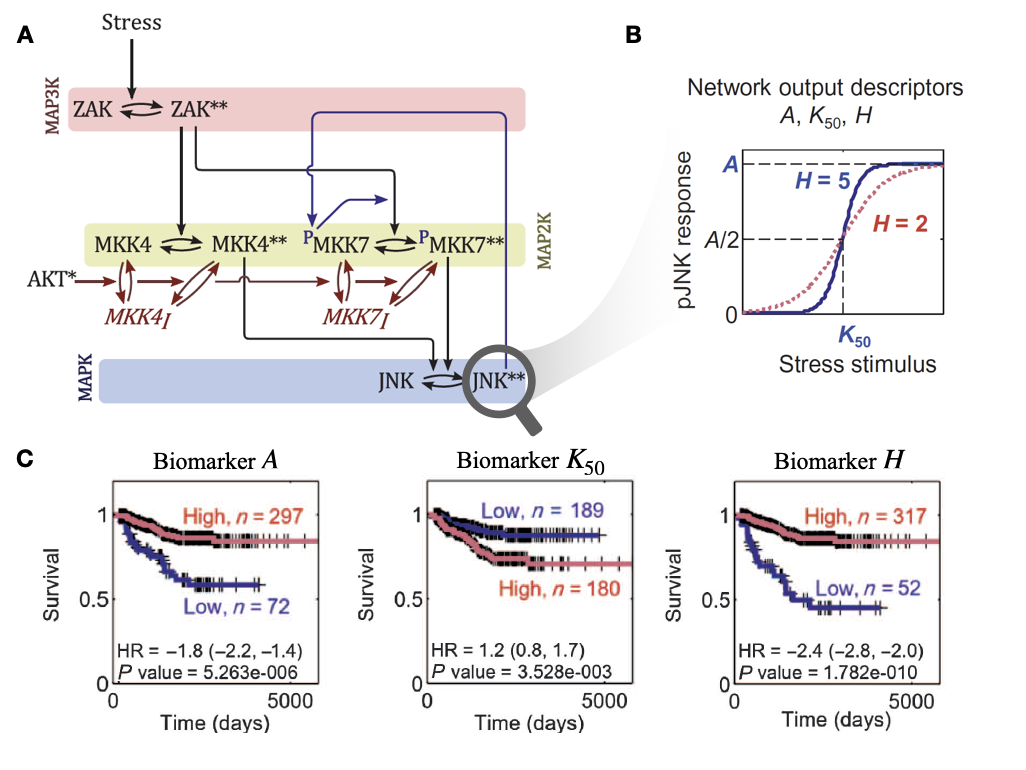
\includegraphics[width=0.9\linewidth]{fig/fey} 

}

\caption[Schematic example of logical and ODE modeling around MAPK signaling]{\textbf{Mechanistic modeling of JNK pathway and
survival of neuroblastima patients, as described by
\citet{fey2015signaling}.} (A) Schematic representation, as a process
description, for the ODE model of JNK pathway. (B) Response curve
(phosphorylated JNK) as a function of the input stimulus (Stress) and
characterization of the corresponding sigmoidal function with maximal
amplitude \(A\), Hill exponent \(H\) and activation threshold
\(K_{50}\). (C) Survival curves for neuroblastoma patients based on
binarized \(A\), \(K_{50}\) and \(H\); binarization thresholds having
been defined based on optimization screening on calibration cohort.}\label{fig:fey}
\end{figure}












On the logical modeling side, there are also studies including
prognostic value validation. Thus, \citet{khan2017unraveling} proposed
two logical models of epitelio-mesenchymal transition (EMT) in bladder
and breast cancers. These models are inferred from prior mechanisms
knowledge and data analysis with particular attention to potential
feedback loops. Using these models, it is possible to study the
behaviour of them for all combinations of model inputs (growth factors
and receptor proteins) and derive subsequent signatures for good or bad
prognosis. These signatures are later validated with cohorts of
patients. In this case, the mechanistic model does not seek to capture a
dynamic behavior but to facilitate and \textbf{make understandable the
exploration of combinations of input signals that grow exponentially
with the number of inputs considered}. Other formalisms, called pathway
activity analysis and following the same activity flows principles
(Figure \ref{fig:toyraf}A), have been analysed in the light of their
prognostic value. Their greater flexibility enables the direct use of
networks of several hundred or thousands of genes, such as those present
in the KEGG database \citep{kanehisa2012kegg}. The benefit of
mechanistic modeling is then to organize high-dimensional data and to
facilitate the \emph{a posteriori} analysis of the results.

\subsection{Predictive models}\label{predictive-models}

But the explicit representation of biological entities in mechanistic
models makes them particularly \textbf{suitable for the study of
well-defined perturbations such as drug effects}. Indeed, by assuming
that the mechanism of action of a drug is at least partially known, it
is possible to integrate this mechanism into the model if it contains
the target of the drug (Figure \ref{fig:netdrug}). One can therefore
simulate the effect of one drug or even compare several. These
strategies have already been implemented in a qualitative way with
logical models used to explain resistance to certain treatments of
breast cancer \citep{zanudo2017network} or even highlight the synergy of
certain combinations of treatments in gastric cancer
\citep{flobak2015discovery}. The value of these models, however, is more
scientific than clinical in that they focus on a single cell line or a
restricted group of cell lines. The possibility to personalize the
predictions or recommendations for different molecular profiles of cell
lines or patients is therefore not obvious. Still within the context of
logical formalism, \citet{knijnenburg2016logic} proposed a broader
approach: if their model needs to be trained, it can nevertheless
provide an analytical framework for several hundred cell lines, while
remaining within the scope of the training data to ensure the validity
of predictions.

\begin{figure}

{\centering 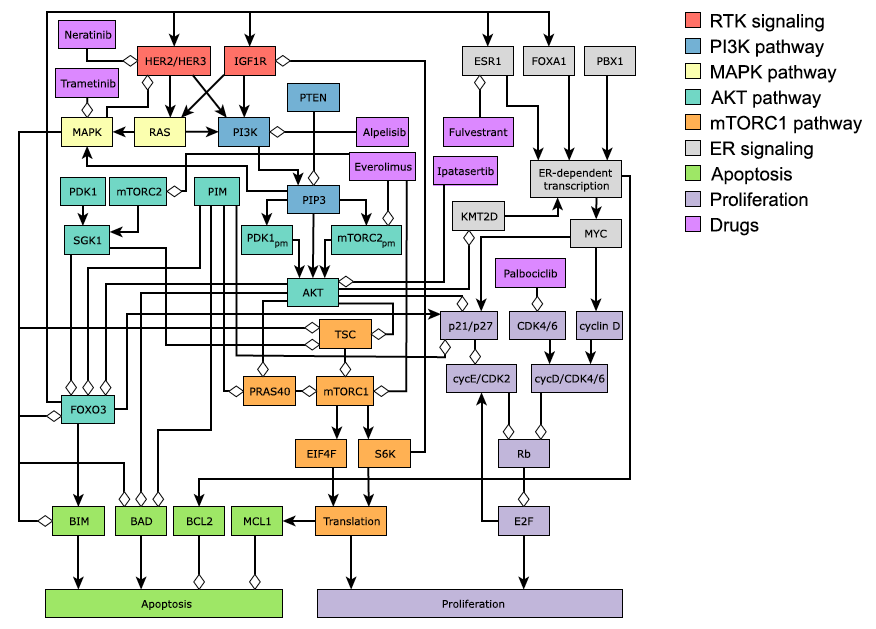
\includegraphics[width=0.9\linewidth]{fig/netdrug} 

}

\caption[Network model of oncogenic signal transduction in ER+ breast cancer, including some drugs and their targets]{\textbf{Network model of oncogenic signal
transduction in ER+ breast cancer, including some drugs and their
targets.} Reprinted from \citet{zanudo2017network}.}\label{fig:netdrug}
\end{figure}





Conceptually comparable strategies can be found on the side of
differential equations where large mechanical models of cell signalling
are also trained to predict the response to different treatments
\citep{bouhaddou2018mechanistic, frohlich2018efficient}. A calibrated
model can then predict the response to a combination of treatments not
tested in the training data, thereby proving the ability of mechanistic
models to extend their predictive value beyond the data
\citep{frohlich2018efficient}. As with prognostic models, mechanical
approaches other than logical formalisms and ODEs have been proposed and
validated \citep{jastrzebski2018integrative}. What can be learned from
these predictive models is that they require \textbf{significant
training data to be able to go beyond qualitative predictions and
dissect treatment response mechanisms of many cell lines
simultaneously}. For obvious practical and ethical reasons, the
validation of these models is for the moment limited to preclinical data
since they require data for many uncertain therapeutic interventions.

This first bridge between mechanistic models of cell signalling and
clinical applications concludes this introductory part. The next part
will be devoted to the definition of new methods to establish this
connection based on logical formalism, before the third part proposes a
more statistical evaluation of the prognostic and predictive values of
the models presented in the previous parts.

\part{Personalized logical models of
cancer}\label{part-personalized-logical-models-of-cancer}

\chapter{Logical modeling principles and data
integration}\label{logical-modeling-principles-and-data-integration}

\epigraph{"Je suis l’halluciné de la forêt des Nombres.

Ils me fixent, avec leurs yeux de leurs problèmes ;

Ils sont, pour éternellement rester : les mêmes.

Primordiaux et définis,

Ils tiennent le monde entre leurs infinis ;

Ils expliquent le fond et l’essence des choses,

Puisqu’à travers les temps planent leurs causes."}{Émile Verhaeren (Les nombres)}

\initial{A}nother way of ordering the diversity of mechanistic models
presented above is to consider their relationship to biological data.
Those that make little use of these data are essentially theoretical
scope models that describe the general functioning of signaling pathways
and associated systems \citep{calzone2010mathematical}. Other models
propose more quantitative models but require much more data, either from
databases or experimental data generated for this purpose in order to
fit the parameters. In the latter case, the necessary data is usually
perturbation data: how does my system react to this or that inhibition
or activation? For a single cell line this already corresponds to a
large amount of data \citep{razzaq2018computational}. And if we want to
extend these approaches to many cell lines, the amount of data becomes
massive \citep{frohlich2018efficient}. For patient-specific models,
access to this perturbation data is even more difficult.

Between theoretical models that are not very demanding in terms of data
but not very applicable clinically and models with a clinical focus but
very demanding in terms of data, an intermediate alternative is missing.
\textbf{Can patient-specific mechanistic models be developed that would
provide qualitative clinical interpretation with a small amount of data,
accessible even in patients?} In this part, composed of three chapters,
a middle way will be described to answer positively to this question.
This methodology will be based on a historically qualitative
mathematical formalism already presented in the previous chapter under
the name of logical modeling. Logical modeling in general will be
detailed in this chapter before describing an original personalized
approach in the next two chapters.

\BeginKnitrBlock{summarybox}
\subsubsection*{Publications}\label{publications}
\addcontentsline{toc}{subsubsection}{Publications}

This chapter presents the theoretical bases of logical modeling and the
tools used thereafter. It does not present any original work but refers
to the synthesis and analyses of logical modeling as described in
\citet{beal2019personalization} and \citet{beal2020modelisation}.
\EndKnitrBlock{summarybox}

\section{Logical modeling paradigms for qualitative
description}\label{logical-modeling-paradigms-for-qualitative-description}

Mathematical models serve as tools to answer a biological question in a
formal way, to detect blind spots and thus better understand a system,
to organize, into a consensual and compact manner, information dispersed
in different articles. In the light of this definition, logical
formalism (also called Boolean) may seem one of the closest to natural
language in that it \textbf{can translate quite directly the statements
present in the literature} such as ``protein A activates protein B'' or
``the expression of gene C requires the joint presence of factors D and
E''. Indeed, shortly after the first descriptions of control circuits by
\citet{jacob1961genetic}, the interest of logical models to describe
biological systems was put forward by \citet{kauffman1969homeostasis}
and \citet{thomas1973boolean}. Since then, studies have multiplied
\citep{thomas1990biological}, varying the fields of biological
applications and also the mathematical and computational implementations
\citep{naldi2018colomoto}. The two subsections below summarize the
characteristics common to most of the logical formalisms, before
detailing the implementation chosen in this thesis in section
\ref{maboss-section}. A review of the use of data in logic models will
finally be proposed in section \ref{logical-data-section}.

\subsection{Regulatory graph and logical
rules}\label{regulatory-graph-and-logical-rules}

A logical model is based on a network called \textbf{regulatory graph}
(Figure \ref{fig:logical}), where each \textbf{node} represents a
component (e.g.~genes, proteins, complexes, phenotypes or processes),
and is associated with discrete levels of activity (\(0\), \(1\), or
more when justified). The use of a discrete formalism in molecular
network modeling relies on the highly non-linear nature of regulation,
and thus on the existence of a regulatory threshold. Assuming that each
variable represents a level of expression, it will take the value \(0\)
if the level of expression of the entity is below the regulation
threshold, i.e., insufficient to carry out the regulation; and the value
\(1\) if it is above the threshold and regulation is possible. In other
words, the control threshold discretizes the state space, here the
expression levels. It is therefore possible to distinguish several
thresholds for the same variable, corresponding to distinct controls
that do not take place at the same expression levels. The variable is
then multivalued. This extension greatly enriches the formalism, because
it allows to distinguish situations that are qualitatively different and
that would be confused with Boolean variables. In the continuation of
this thesis, we will consider by default that the activity levels are
binary, \(0\) corresponding to an inactive entity and \(1\) to an active
entity. The \textbf{edges} of this regulatory graph correspond to
influences, either positive or negative, which illustrate the possible
interactions between two entities (Figure \ref{fig:logical}). Positive
edges can represent the formation of active complexes, mediation of
synthesis, catalysis, etc. and they will be later depicted as green
arrows (\(\leftarrow\)). Negative edges on the other hand can represent
inhibition of synthesis, degradation, inhibiting (de)phosphorylation,
etc. and they will be depicted as red turnstile (\(\vdash\)).

\begin{figure}

{\centering 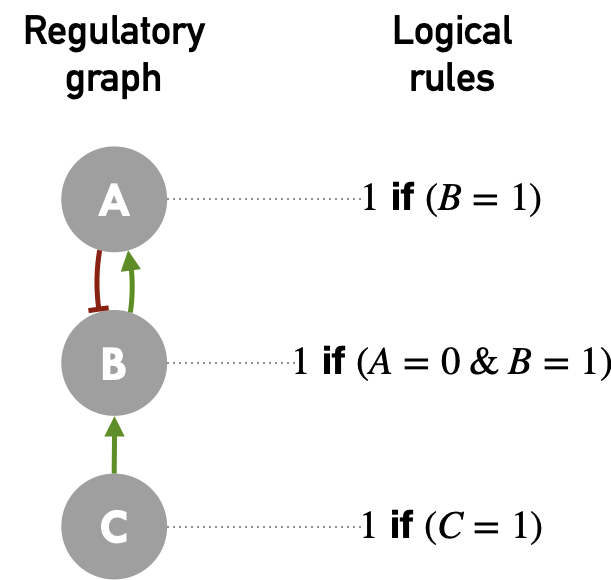
\includegraphics[width=0.5\linewidth]{fig/logical} 

}

\caption[A simple example of a logical model]{\textbf{A simple example of a logical model.}
Regulatory graph on the left with positive (green) and negative
regulations (red); a set of possible corresponding logical rules on the
right.}\label{fig:logical}
\end{figure}






Then, each node of the regulatory graph has a corresponding Boolean
variable associated to it. The variables can take two values: \(0\) for
absent or inactive (OFF), and \(1\) for present or active (ON). These
variables change their value according to a logical rule assigned to
them. The state of a variable will thus depend on its \textbf{logical
rule}, which is based on logical statements, i.e., on a function of the
node regulators linked with logical connectors AND (\(\&\)), OR (\(|\))
and NOT (\(!\)). These operators can account for what is known about the
biology behind these edges. If two input nodes are needed for the
activation of the target node, they will be linked by an AND gate; to
list different means of activation of a node, an OR gate will be used;
and negative influences will rely on NOT gates. The rules corresponding
to the toy model in Figure \ref{fig:logical} could be interpreted
literally like this: A is acivated to 1 if B is active; B is updated to
1 in the absence of A and the presence/activity of C; C is an input of
the model and therefore not regulated. It can be noted that the logical
rules cannot be deduced only from the regulatory graph, which can be
less precise and ambiguous. One could thus imagine that B is activated
if C is, OR if A is not, thus changing the behavior of the model.

\subsection{State transition graph and
updates}\label{state-transition-graph-and-updates}

In a Boolean framework, the variables associated to each node can take
two values, either \(0\) or \(1\). We define a model state as a vector
of all node states. All the possible transitions from any model state to
another are dependent on the set of logical rules that define the model.
These transitions can be viewed into a graph called a \textbf{state
transition graph} (STG), where nodes are model states and edges are the
transitions from one model state to another. STG nodes will be later
depicted with rounded squares instead of circles in order to emphasize
the difference with regulatory graphs. That way, trajectories from an
initial condition to all the final states can be determined. In a model
with \(n\) nodes, the STG can contain up to \(2^n\) model state nodes;
thus, if \(n\) is too big, the construction and the visualization of the
graph becomes difficult.

\begin{figure}

{\centering 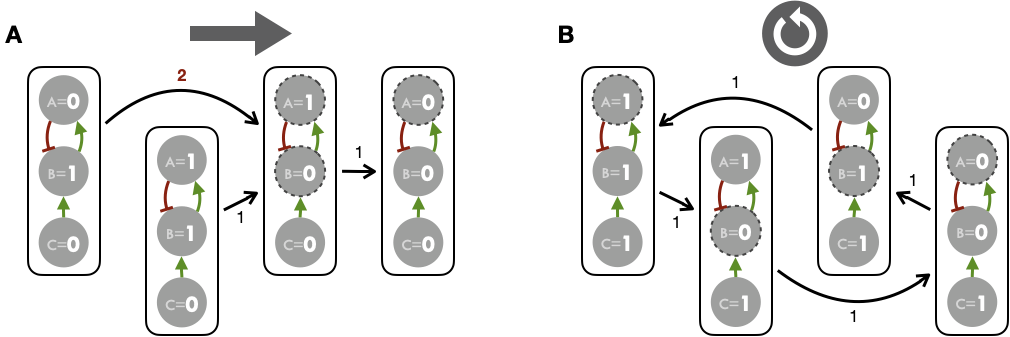
\includegraphics[width=0.9\linewidth]{fig/synchronous} 

}

\caption[A simple example of a logical model]{\textbf{State transition graph and synchronous
updates.} Stable state (A) and limit cycle (B) attractors obtained for
the example logical model with synchronous updates (all possible updates
simultaneously). Figures above/below STG edges correspond to the number
of nodes updated in each transition.}\label{fig:synchronous}
\end{figure}







Based the simple logical model of Figure \ref{fig:logical} it is
nevertheless possible to represent the STG comprehensively. The idea for
this is to start from a state of the system and track the successive
states defined by the logical rules and the corresponding updates. The
first strategy to construct this STG is to change simultaneously at each
time step all the variables that can be changed (Figure
\ref{fig:synchronous}). This method is referred to as a
\textbf{synchronous updating strategy}. In the second method, referred
to as a \textbf{asynchronous updating strategy}, variables are changed
one at a time (Figure \ref{fig:asynchronous}) and therefore each state
has as many successors as there are components whose state must be
changed according to logical rules (Figure \ref{fig:asynchronous}A). The
latter asynchronous method will be used exclusively in the work
presented thereafter.

\begin{figure}

{\centering 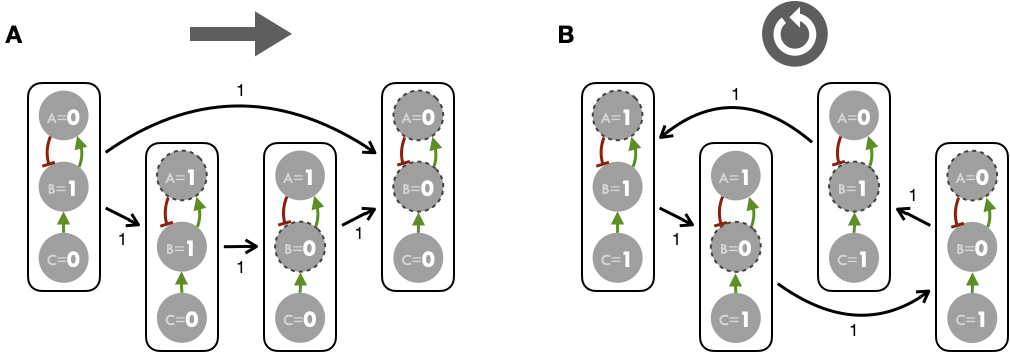
\includegraphics[width=0.9\linewidth]{fig/asynchronous} 

}

\caption[A simple example of a logical model]{\textbf{State transition graph and
asynchronous updates.} Stable state (A) and limit cycle (B) attractors
obtained for the example logical model with asynchronous updates (one
update at a time). Figures above/below STG edges correspond to the
number of nodes updated in each transition.}\label{fig:asynchronous}
\end{figure}







We then define attractors of the model as long-term asymptotic behaviors
of the system. Two types of attractors are identified: stable states,
when the system has reached a model state whose successor in the
transition graph is the model state itself; and cyclic attractors, when
trajectories in the transition graph lead to a group of model states
that are cycling. For both synchronous and asynchronous updating
strategies, the toy model shows the existence of \textbf{two types of
attractors: a stable steady state and a limit cycle}, depending on the
initial value of \(C\). There are two disconnected components of the STG
for this example that correspond to the two possible values for the
input \(C\). If \(C\) is initially equal to 0 (inactive), then there
exists only one stable state: \(A=B=C=0\). All the trajectories in the
state transition graph lead to a single final model state. If \(C\) is
initially equal to 1, then the attractor is a limit cycle. The path in
the STG cycles for any initial model state of this connected component.
Note that for the asynchronous and synchronous graphs, the precise paths
or limit cycles may differ. To conclude, it is important to emphasize
and illustrate the characteristics of asynchronous updates in this toy
example. In Figure \ref{fig:asynchronous}A, the transition from the
initial state (\(A=C=0;B=1\)) suggests two distinct possibilities, so it
is necessary to \textbf{define additional rules or heuristics to choose
between possible transitions}. We will come back to this by specifying
the logical modeling implementation chosen in this thesis in section
\ref{maboss-section}.

\subsection{Tools for logical
modeling}\label{tools-for-logical-modeling}

Numerous tools have been developed to build logical models and study the
dynamics of the systems under investigation, each with its own
specificity. They allow, for example, to represent regulation networks;
to edit, modify or infer logical rules; to identify stable states; to
reduce models; to visualize graphs of synchronous or asynchronous
transitions. Some also allow to integrate temporal data; to discretize
expression data; to simulate the model stochastically or to integrate
delays; to identify existing models, etc. Among them, we can cite GINsim
\citep{naldi2018logical}, BoolNet \citep{mussel2010boolnet}, pyBoolNet
\citep{klarner2016pyboolnet}, BooleanNet \citep{albert2008boolean},
CellCollective \citep{helikar2012cell}, bioLQM \citep{naldi2018biolqm},
MaBoSS \citep{stoll2012continuous, stoll2017maboss}, PINT \citep{Pint},
CaspoTS \citep{ostrowski2016boolean}, or CellNOptR
\citep{terfve2012cellnoptr}. The interaction between all these tools,
their interoperability and complementarity are highlighted in the form
of a notebook jupyter \citep{naldi2018colomoto}, and some of them are
described in more details in section \ref{logical-data-section}.

\section{The MaBoSS framework for logical
modeling}\label{maboss-section}

In the present study, all simulations have been performed with MaBoSS, a
\textbf{Ma}rkovian \textbf{Bo}olean \textbf{S}tochastic
\textbf{S}imulator whose design is summarized in Figure \ref{fig:maboss}
and precisely described by \citet{stoll2012continuous} and
\citet{stoll2017maboss}. This framework is based on an asynchronous
update scheme combined with a continuous time feature obtained with
Gillespie algorithm \citep{gillespie1976general}, allowing simulations
to be continuous in time despite the discrete nature of logical
modeling.

\begin{figure}

{\centering 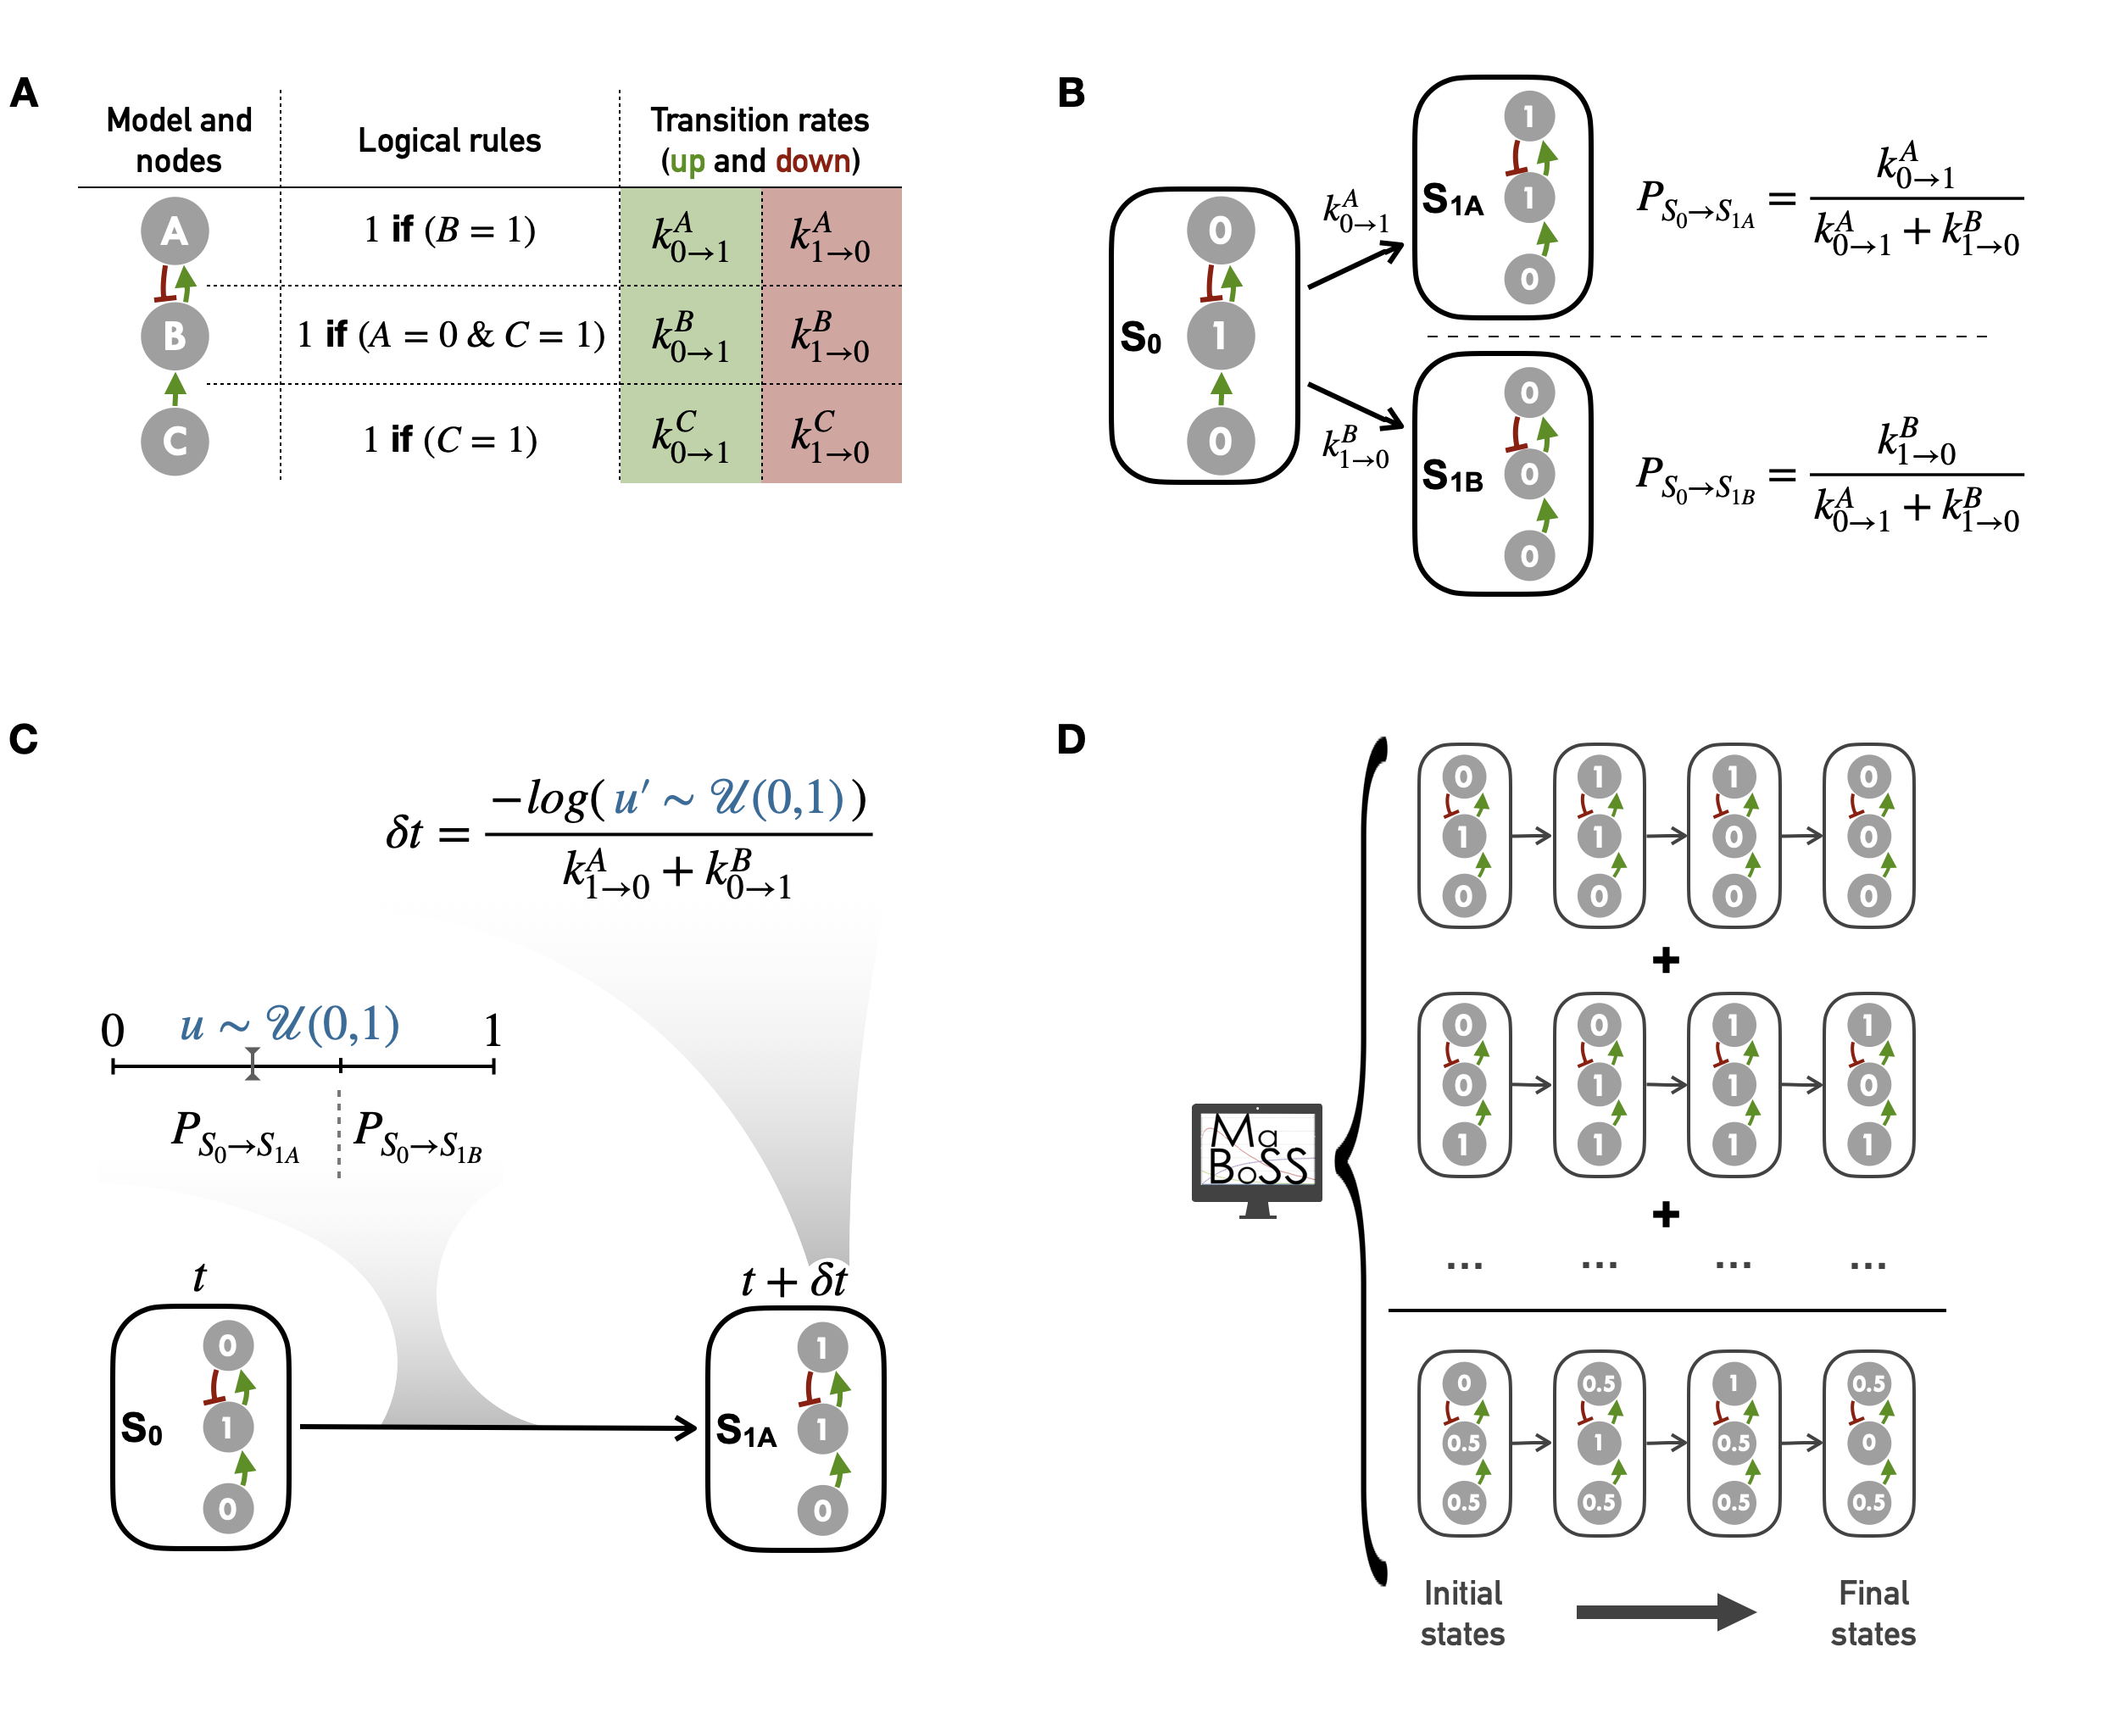
\includegraphics[width=1\linewidth]{fig/maboss} 

}

\caption[Main principles of MaBoSS simulation framework and Gillespie algorithm]{\textbf{Main principles of MaBoSS simulation
framework and Gillespie algorithm.} (A) A logical model with regulatory
graph, logical rules and transition rates. (B) A corresponding state
transition graph with two possible transitions in asynchronous update
for a given initial state; each transition has an associated
probability. (C) Random selection of a specific transition and time by
the Gillespie algorithm from two uniform random variables. (D) Schematic
representation of a logical model simulation with MaBoSS: average
trajectory obtained from the mean of many individual stochastic
trajectories.}\label{fig:maboss}
\end{figure}












\subsection{Gillespie algorithm}\label{gillespie-algorithm}

Gillespie algorithm provides a \textbf{stochastic way to choose a
specific transition among several possible ones} and to infer a
corresponding time for this transition. Thus, MaBoSS computation results
in one stochastic trajectory as a function of time. To achieve this,
transition rates seen as qualitative activation or inactivation rates,
must be specified for each node (Figure \ref{fig:maboss}A). They can be
set either all to the same value by default, in the absence of any
indication, or in various levels reflecting different orders of
magnitude: post-translational modifications are quicker than
transcriptions for instance. These transition rates are translated as
\textbf{transition probabilities} in order to determine the actual
transition (Figure \ref{fig:maboss}B). Indeed, the probability for each
possible transition to be chosen for the next update is the ratio of its
transition rate to the sum of rates of all possible transitions. Higher
rates correspond to transitions that will take place with greater
probability, or in other words more quickly.

Thus at each update, the Gillespie algorithm performs the procedure
described in Figure \ref{fig:maboss}C. Two uniform random variables
\(u\) and \(u'\) are drawn and used respectively to select the
transition among the different possibilities (with \(u\)) and to infer
the corresponding time (with \(u'\)). Based on the described formula,
time \(\delta t\) follows an exponential law whose average is equal to
the inverse of the sum of all possible transition rates (Figure
\ref{fig:maboss}C). In present work, except otherwise stated, all
transition states will be initially assigned to 1.

\subsection{A stochastic exploration of model
behaviours}\label{a-stochastic-exploration-of-model-behaviours}

Since MaBoSS computes stochastic trajectories, it is relevant to compute
several trajectories in order to get an insight of the average behavior
by generating a \textbf{population of stochastic trajectories} over the
asynchronous state transition graph (Figure \ref{fig:maboss}D). The
aggregation of stochastic trajectories can also be interpreted as a
description of an heterogeneous population. In fact, in all the examples
in next chapters, all simulations have consisted thousands of computed
trajectories. The larger the model, the larger the space of
possibilities and the more trajectories are required to explore it.
Since several trajectories are simulated, initial values of each node
can be defined with a continuous value between 0 and 1 representing the
probability for the node to be defined to 1 for each new trajectory. For
instance, a node with a \(0.6\) initial condition will be set to \(1\)
in \(60\%\) of simulated trajectories and to \(0\) in \(40\%\) of the
cases.

In the present work, we will focus on the \emph{asymptotic} state of
these simulations instead of transient dynamics and we will call
\textbf{node scores} the asymptotic agregated score obtained by
averaging all trajectories at a given final time point. Indeed,
asymptotic states are more closely related to logical model attractors
than transient dynamics and are therefore less dependent on updating
stochasticity and more biologically meaningful \citep{huang2009cancer}.
Note that the simulation time should be chosen carefully to ensure that
the asymptotic state is achieved, and the term \emph{final state} may be
considered as safer. All in all this modeling framework is at the
intersection of logical modeling and continuous dynamic modeling. If the
definition of time remains rather abstract and difficult to interpret
experimentally, the stochastic exploration of trajectories makes it
possible to refine the purely binary interpretation of the variables.

\subsection{From theoretical models to data
models?}\label{from-theoretical-models-to-data-models}

To sum up, logical formalism makes it possible to design fairly quickly
and easily models that reflect \emph{a priori} knowledge of the
phenomena being studied. Thus, they allow answering questions for which
there is little information on the precise mechanisms involved in a
disease or when there is a lack of data related to the expression of
genes or the quantity of key proteins, or on the speed of certain
processes. Logical models can confirm that a network is a good
illustration of the underlying biological question. However, in order to
propose a patient-specific mechanistic approach, it seems crucial to use
the biological data available. How is this possible in a formalism that
is by definition quite abstract?

\section{Data integration and semi-quantitative logical
modeling}\label{logical-data-section}

The higher level of abstraction of the logical formalism sometimes makes
the necessary back and forth between theoretical modeling and
experimental or clinical data less easy. However, many theoretical
approaches have been developed over the years to enable this dialogue at
all stages, from the construction to the validation of a logical model,
as summarized in Figure \ref{fig:logical-data}. This section summarizes
some of these approaches to show \textbf{how the use of biological data
enriches logical models and brings them closer to clinical applications}
in precision medicine. The purpose of this presentation is also to
better contextualize the original approach presented in the following
chapter. It should be noted that the methods presented below are all
applicable to logical models, and illustrated with such examples where
possible. However, some methods are not specific to this formalism and
can be applied to other modeling frameworks.

\begin{figure}

{\centering 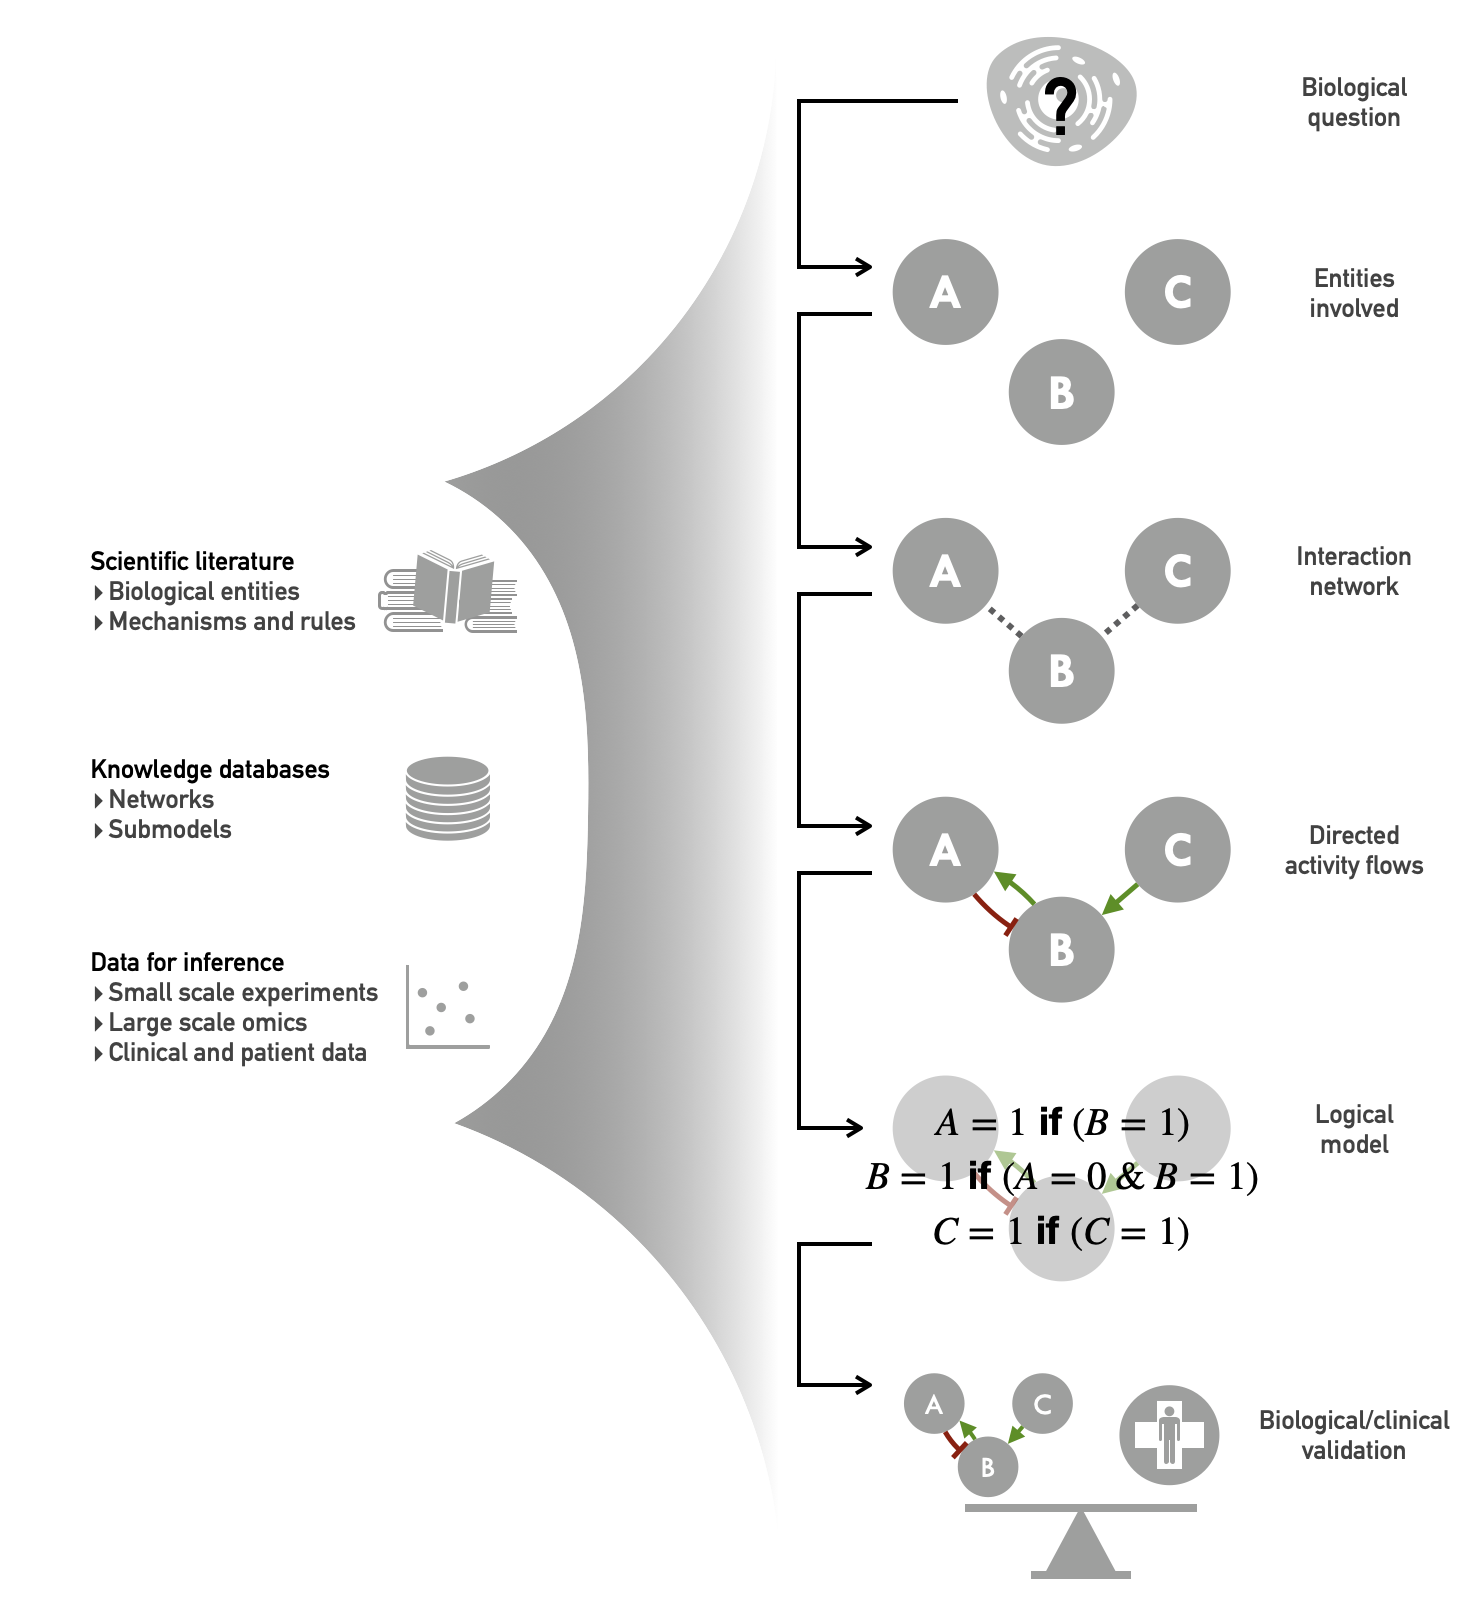
\includegraphics[width=0.9\linewidth]{fig/logical-data} 

}

\caption[Main principles of MaBoSS simulation framework and Gillespie algorithm]{\textbf{Data integration in logical
modeling.} The main types of data used are shown on the left; the
essential steps of the logical modeling are shown linearly on the right.}\label{fig:logical-data}
\end{figure}





\subsection{Build the regulatory
graph}\label{build-the-regulatory-graph}

Faced with a biological question (Figure \ref{fig:logical-data}, first
step), it is crucial to identify the main actors in the process in order
to \textbf{define the outline of the model} (Figure
\ref{fig:logical-data}, second step). A first approach relies on the
existing scientific literature on the topic: which biological species
and which interactions have been identified as relevant to my problem?
In a more automatic way, it is possible to extract information from
different databases in order to establish an initial list of biological
entities and interactions associated with a biological phenomenon or
even a gene of interest \citep{kanehisa2012kegg, perfetto2016signor}. As
an example, starting from the study of E2F1 gene as the hub of many
regulatory mechanisms, \citet{khan2017unraveling} have reconstructed a
dense network of interactions in the vicinity of E2F1, which will be
used for the construction of their subsequent model. The main difficulty
here is to choose and select the relevant biological information adapted
to the context of the model to be created, depending for example on the
type of cancer studied or the desired level of precision.

But if the literature can be considered as processed data, it is also
possible to use directly experimental data related to the problem under
study. Key actors of biological processes identified by statistical
analysis, such as differentially expressed genes or the most frequently
mutated genes in a patient cohort, are selected and used as a starting
point for the construction of the model \citep{remy2015modeling}. More
comprehensive approaches can use differential analysis tools on
signaling pathways, rather than individual genes, to choose the relevant
processes to include by contrasting different groups of patients based
on their grades, metstatic status, resistance to treatments etc.
\citep{martignetti2016roma, montagud2017conceptual}. Similarly, the
study of regulatory networks involving transcription factors may justify
the use of ChIP-seq data to identify possible new transcriptional
regulations not previously listed \citep{collombet2017logical}.

Once the main actors have been identified, it is necessary to
\textbf{infer the links} between them (Figure \ref{fig:logical-data},
third and fourth step). However, starting from a list of genes and
proteins of interest, how can we ensure that the regulatory
relationships are complete and relevant? While a careful reading of the
literature can provide locally interesting information, the use of omics
data is also a resource that can be declined to different levels of
precision. The major interest of these methods, assuming that the data
are adequate and sufficiently massive, is to be able to extract
information as large as the dataset, potentially on hundreds of
entities, and above all specific to the object of study: a cancer
subtype or a particular cell line can thus generate their own
interaction network \citep{lefebvre2010human}. Inference methods extract
biological knowledge hidden in large databases, summarize it and
represent it via networks. Many methods construct coexpression networks,
which are non-oriented graphs, with different metrics and methods
\citep{margolin2006aracne, vert2007new}. Other approaches seek to infer
causal relations between components, allowing the reconstruction of
directed graphs where the links between entities are oriented, and
sometimes even signed as activating (positive) or inhibiting (negative)
regulations. These methods often make use of time series
\citep{hill2016inferring} or perturbation data
\citep{meinshausen2016methods}, but also more recently from
observational data \citep{verny2017learning}. The information extracted
from the data is then directly readable in the form of activity flows as
described in the SBGN standards \citep{novere2009systems}, thus
providing a representation adapted to the construction of qualitative
models and \emph{a fortiori} of logical models
\citep{le2015quantitative}. Closer to the objective of defining logical
models, certain methods allow the study and inference of co-regulation
expressed with logical operators \citep{elati2007licorn}, thus
facilitating the passage from the definition of an interaction network
to the construction of a true logical model.

\subsection{Define the logical rules}\label{define-the-logical-rules}

Precision must then be taken further by defining the logical rules that
complete the network (Figure \ref{fig:logical-data}, fifth step). The
first source of aggregated data to define logical rules is the
scientific literature. The modeler looks for the state of knowledge on a
given regulatory mechanism and translates it into a \textbf{local
logical rule}, according to the desired level of precision. For example,
it has been observed that the protein kinase AKT can stabilize the
oncogene MDM2 by phosphorylation, which leads to the degradation of p53
by forming a complex with it: this example can be translated by a simple
inhibition relationship of AKT on p53 if this level of precision is
considered sufficient or else intermediate species such as MDM2 can be
used \citep{cohen2015mathematical}. Then, the effect of inhibition must
be defined: can MDM2 alone inhibit p53 or does the presence of other
activators outweigh this effect? This kind of considerations allows to
define the logical combinations between the different inputs of a
network node. In some cases, experimental data can be used to answer
such questions: is a single activator sufficient or is the presence of
all activators necessary? Which of the activator or inhibitor prevails
in the case of simultaneous presence? While this information is often
found in the literature, one should generate one's own experimental data
to ensure an answer tailored to the study context, using a variety of
experimental molecular biology techniques. For example, in order to
elucidate the relationship between Foxo1 and Cebpa in a model of
differentiation of myeloid and lymphoid cells,
\citet{collombet2017logical} first established the physical relationship
between these species by ChIP-seq before determining the nature of this
relationship using an ectopic expression experiment of Foxo1 in
macrophage cells.

Other, more global approaches have been developed in recent years,
driven by the influx of data from high-throughput sequencing techniques.
Based on this rich and complex data, it has become possible to
\textbf{infer entire logical models, with precisely defined rules and
interactions} \citep{ostrowski2016boolean}. The algorithms CellNOpt
\citep{terfve2012cellnoptr} and caspo \citep{videla2017caspo} provide
two examples of these approaches, and more recently the SCNS tool
described a graphical interface to infer logical models from single cell
data \citep{woodhouse2018scns}. This model-inference goes beyond simpler
structure-inference by defining the logical rules, but it is generally
based on a predefined topological structure to which time series or
perturbation data are added. These data provide access to the response
dynamics of a system. By questioning the way the system reacts, these
data are therefore richer than a snapshot and thus facilitate the
transition from correlation to causality, and thus the inference of
logical rules. In practice, the use of proteomic or phospho-proteomic
data is often recommended because these data account for the activity of
the protein and are in fact the closest to the cellular response
\citep{ostrowski2016boolean, terfve2012cellnoptr, terfve2015largescale}.
In spite of the richness of this type of data, model inference is
sometimes still an under-determined problem that can lead to a large
number of models with different logical rules equally compatible with
the data. In such situations, it is then a matter of choosing the model
on the basis of biological relevance criteria or of accepting to use
families of models instead of limiting oneself to a single model
\citep{videla2017caspo}. In all cases, constructing logical rules
directly from data specific to the problem can make it possible to
obtain logical rules that are also specific to the context or the system
under study \citep{saezrodriguez2011comparing}. For example, the
inference of logical models specific to one or some cancer cell lines is
a powerful tool to study their particularities
\citep{razzaq2018computational}.

\subsection{Validate the model}\label{validate-the-model}

Finally, the data can be used to validate the \textbf{biological or
clinical relevance of the models} (Figure \ref{fig:logical-data}, sixth
step). Compared to a system of differential equations, logical modelling
has the particularity of being more abstract and therefore less directly
reliable to an experimental reality for its validation. A system of
differential equations can be compared to the chemical kinetics of the
biological system under study. Compared to continuous formalisms, the
dynamics of logic model simulation is more difficult to take into
account but it is possible to verify it qualitatively, for example by
validating the cyclic nature of activation trajectories for a model
simulating the cell cycle \citep{faure2006dynamical} or cellular
decisions as a function of the activation signal
\citep{calzone2010mathematical}. A second, more frequent approach
consists in looking at the model's steady states and associating them
with physiological conditions
\citep[\citet{cohen2015mathematical}]{weinstein2017network}. Finally, a
third strategy focuses on the asymptotic state reached during the
stochastic simulation of the model(s), a state representing a mixture of
the different steady states according to the probability that the model
has of reaching them.

In many models, to facilitate the analysis, \textbf{nodes representing
phenotypes have been added as ``read-out'' of the activity of certain
entities}. Thus, if a model includes a node named \emph{Proliferation},
it will then be simpler to draw interpretations from the simulations
performed with the model that will be linked to experimental
observations of tumor growth or cell proliferation
\citep{grieco2013integrative, steinway2015combinatorial}. To validate
these models, the activity of phenotypes when forcing some node activity
to \(0\) or \(1\) is compared with the results of gene mutations
reported in experiments carried out on mice or cell lines
\citep{faure2006dynamical, cohen2015mathematical}. Another similar
method for validating the relevance of a logical model is based on the
analysis of the effects of different therapeutic molecules. The
mechanistic nature of logical modeling makes it relatively easy to
simulate the effect of these molecules. It is possible to simulate the
effect of an inhibitory molecule by forcing the activity of its target
to 0 and to compare with data
\citep{zanudo2017network, iorio2016landscape, knijnenburg2016logic}.

Beyond validation, some studies have predicted \textbf{new therapeutic
targets} based on logical models, for instance by pointing out
weaknesses in the topology of a regulatory system
\citep{sahin2009modeling}. Taking advantage of the ease of modeling and
multiplying combinations of therapeutic molecules, logical modeling has
also proved fruitful in predicting the best therapeutic combinations and
their synergies, in the context of gastric cancers for example
\citep{flobak2015discovery}. Experimental confirmation of the
predictions resulting from the modeling is then the ultimate stage in
the validation of a logical model, completing the fruitful round trip
between models and data.

\chapter{Personalization of logical models: method and prognostic
validation}\label{personalization-of-logical-models-method-and-prognostic-validation}

\epigraph{"All happy families are alike; each unhappy family is unhappy in its own way."}{Leo Tolstoy (Anna Karenina, 1877)}

\initial{N}ow that logical modeling has been introduced, it is possible
to come back to the question that structures this part and to refine it.
\textbf{Is it possible to use routine omics data to obtain logical
models that provide qualitative clinical interpretation?}. We thus
propose a sequential approach, separating the model construction process
from the integration of biological data. A generic logical model is
first built, based on the literature knowledge, and the data are then
used to specify the model. Indeed, the model as defined from the
literature is often generic in the sense that it summarizes the state of
knowledge on a probably heterogeneous pathology or population. Assuming
that this general regulatory scheme provides a relevant framework for
the system, it may then be relevant to use more precise omics data to
impose biologically sourced constraints on the model: inactivation of a
gene in a patient, activation of a protein or a signalling pathway by
overexpression or phosphorylation, etc. This approach, called
\textbf{PROFILE} (PeRsonalization OF logIcaL ModEls), allows the
integration of both discrete (mutations) and continuous data (RNA
expression levels, proteins) based on the MaBoSS software, and leads to
specific models of a cell line or a patient.

\BeginKnitrBlock{summarybox}
\subsubsection*{Publications}\label{publications-1}
\addcontentsline{toc}{subsubsection}{Publications}

This chapter presents the method developed during the thesis to
personalize logical models, i.e., generate patient-specific models from
a single generic one. The principles of the method and some analyses on
patient data have been comprehensively described in
\citet{beal2019personalization} and briefly summarized in
\citet{beal2020personalized}. Analyses on cell lines are unpublished.
\EndKnitrBlock{summarybox}

\section{From one generic model to data-specific models with PROFILE
method}\label{from-one-generic-model-to-data-specific-models-with-profile-method}

The PROFILE method is summarized in Figure \ref{fig:PROFILE-abstract}
and the different steps are successively described in the following
subsections.

\begin{figure}

{\centering 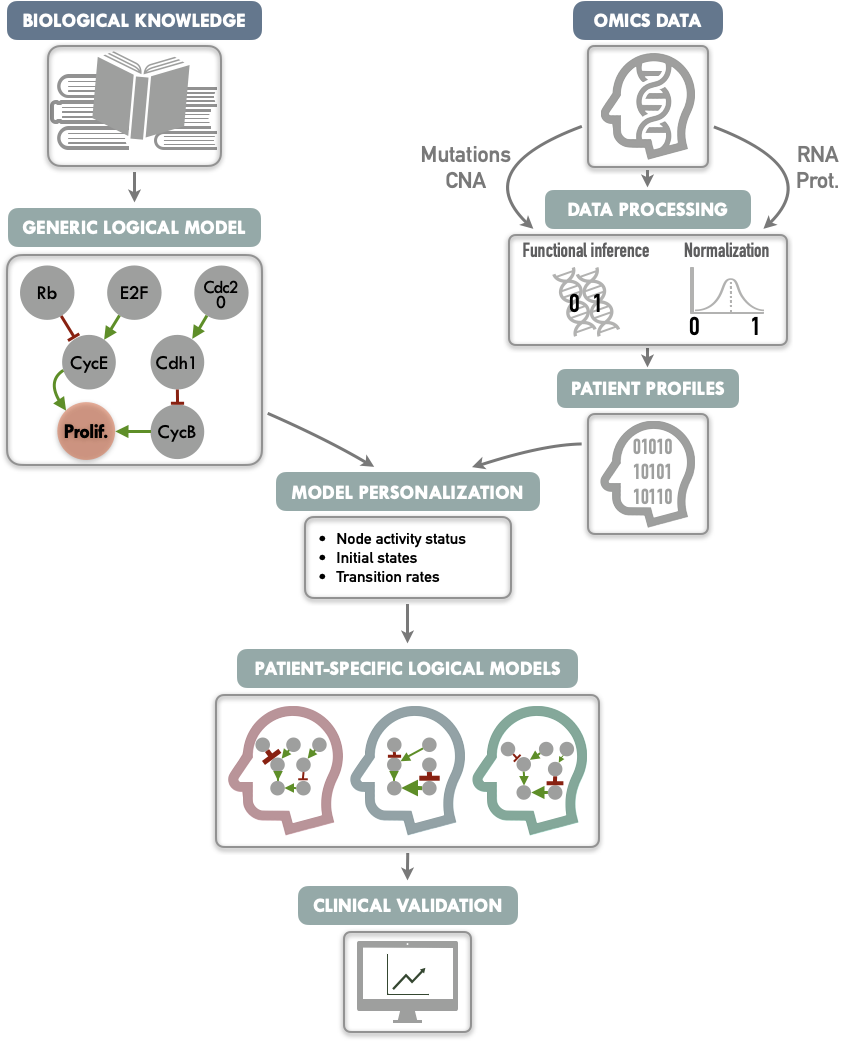
\includegraphics[width=0.8\linewidth]{fig/PROFILE-abstract} 

}

\caption[Graphical abstract of PROFILE method to personalize logical models with omics data]{\textbf{Graphical abstract of PROFILE
method to personalize logical models with omics data.} On the one hand
(upper left), a generic logical model, in a MaBoSS format is derived
from literature knowledge to serve as the starting-point. On the other
hand (upper right), omics data are gathered (e.g., genome and
transcriptome) as data frames, and processed through functional
inference methods (for already discrete genome data) or
binarization/normalization (for continuous expression data). The
resulting patient profiles are used to perform model personalization,
i.e., adapt the generic model with patient data. The merging of the
generic model with the patient profiles creates a personalized MaBoSS
model per patient. Then, biological or clinical relevance of these
patient-specific models can be assessed.}\label{fig:PROFILE-abstract}
\end{figure}















\subsection{Gathering knowledge and
data}\label{gathering-knowledge-and-data}

The first steps are therefore to build a logical model adapted to the
biological question (Figure \ref{fig:PROFILE-abstract}, upper left) and
to collect omics data that will be used to personalize the model (Figure
\ref{fig:PROFILE-abstract}, upper right). The construction of the model
can be based on literature or data (see previous chapter). In the latter
case, the data used to build the model will preferably be distinct from
those used to personalize the model.

\subsubsection{A generic logical model of cancer
pathways}\label{a-generic-logical-model-of-cancer-pathways}

In this chapter, which is essentially methodological in nature, we will
use a \textbf{published logical model of cancer pathways} to illustrate
our PROFILE methodology. It is based on a regulatory network summarizing
several key players and pathways involved in cancer mechanisms: RTKs,
PI3K/AKT, WNT/\(\beta\)-catenin, TGF-\(\beta\)/Smads, Rb, HIF-1, p53 and
ATM/ATR \citep{fumia2013boolean}. The later analyses will be mainly
focused on two read-out nodes, \emph{Proliferation} and
\emph{Apoptosis}. Based on the model's logical rules
\emph{Proliferation} node is activated by any of the cyclins (CyclinA,
CyclinB, CyclinD, and CyclinE) and is, thus, an indicator of cyclin
activity as an abstraction and simplification of the cell cycle
behavior. \emph{Apoptosis} node is regulated by Caspase8 and Caspase9.
This generic model contains 98 nodes and 254 edges. Further details and
visual representation are provided in section \ref{appendix-fumia} and
Figure \ref{fig:Fumia}. Model files are available in MaBoSS format in a
dedicated
\href{https://github.com/sysbio-curie/PROFILE/tree/master/Models/Fumia2013}{GitHub
repository}.

\subsubsection{Cancer data to feed the
models}\label{cancer-data-to-feed-the-models}

In order to showcase the method, \textbf{breast-cancer patient data} are
gathered from METABRIC studies
\citep{curtis2012genomic, pereira2016somatic}. 1904 patients have data
for both mutations, copy number alterations, RNA expression and clinical
status (e.g.~survival). This number rises to 2504 patients if we only
look at the mutations. Additional analyses were also performed based on
the smaller and clinically less complete TCGA breast cancer data
\citep{cancer2012comprehensive}. These are detailed in
\citet{beal2019personalization} but not included in this thesis. A more
comprehensive description of these two databases can be found in section
\ref{appendix-datasets-patients}.

In addition to these examples proposed in the original article, an
application to \textbf{cell line data} is proposed in section
\ref{PROFILE-CL} to link to the next chapters. A cohort of 663 cell
lines from different types of cancer will be used. The data are from
Cell Models Passpors \citep[@][]{van2019cell} and are described in more
detail in the appendix \ref{appendix-cl}. In all cases, samples and cell
lines will sometimes be referred to as patients for the sake of
simplicity.

\subsection{Adapting patient profiles to a logical
model}\label{adapting-patient-profiles-to-a-logical-model}

Before describing precisely the methodologies for using the data to
generate patent-specific models, it is important to understand that
these data will need to be transformed. This is the transformation of
raw omics data into processed profiles that can be used directly in
logical modeling.

\subsubsection{Functional inference of discrete
data}\label{functional-inference-of-discrete-data}

Since the logical formalism is itself discrete, the integration of
discrete data is more straightforward. The most natural idea, used in
many previous works, is to \textbf{interpret the functional effect of
these alterations} and to encode it directly in the model. For instance,
a deleterious mutation is integrated into the model by setting the
corresponding node to \(0\) and ignoring the logical rule associated to
it. For activating mutation, the node is set to \(1\). The main obstacle
is therefore to estimate the functional impact of the alterations in
order to translate them as well as possible in the model.

For mutations, based on the variant classification provided by the data,
inactivating mutations (nonsense, frame-shift insertions or deletions
and mutation in splice or translation start sites) are assumed to
correspond to loss of function mutations and therefore the corresponding
nodes of the model are forced to \(0\). Then, missense mutations are
matched with OncoKB database \citep{chakravarty2017oncokb}: for each
mutation present in the database, an effect is assessed (gain or loss of
function assigned to \(1\) and \(0\), respectively) with a corresponding
confidence based on expert and literature knowledge. Then, mutations
targeting oncogenes (resp. tumor-suppressor genes), as defined in the
2020+ driver gene prediction method \citep{tokheim2016evaluating}, are
assumed to be gain of function mutations (resp. loss of function) and
therefore assigned to \(1\) (resp. \(0\)). To rule potential passenger
mutations out, each automatic assignment of a oncogene/tumor-suppressor
gene muations requires that the effect of the mutation has been
identified as significant by predictive software based on protein
structure such as SIFT \citep{kumar2009predicting} or PolyPhen
\citep{adzhubei2010method}.

For integration of copy number alterations, we use the discrete
estimation of gain and loss of copies from GISTIC algorithm processing
\citep{mermel2011gistic}. The loss of both alleles of a gene (labelled
-2) can thus be interpreted as a 0. Conversely, a significant gain of
copies (labelled +2) denotes a gene that tends to be more highly
expressed although the interpretation is more uncertain.

\subsubsection{Normalization of continuous
data}\label{normalization-of-continuous-data}

The integration of continuous data, such as RNA expression levels, in
logical modeling is more difficult. The stochastic framework of MaBoSS
provides however some possibilities. The main continuous mechanistic
parameters of MaBoSS are the initial conditions of each node (its
initial probability of being activated among the set of simulated
stochastic trajectories) and the transition rates associated with the
nodes (its probability to have its transition performed in an
asynchronous update). In order to facilitate the use of continuous data
through one of these two possibilities, we propose to transform them so
that the \textbf{values are continuous between 0 and 1}, what we will
refer to hereafter as normalized data. \textbf{It is assumed that these
continuous data can be good proxies of biological activity}, 0
corresponding to a very low level of activity of the biological entity
and 1 to a very high level. This assumption will have to be explained
and justified each time: high level of expression of an RNA or
significant phosphorylation of a protein interpreted as continuous
markers of an important biological activity for example.

\begin{figure}

{\centering 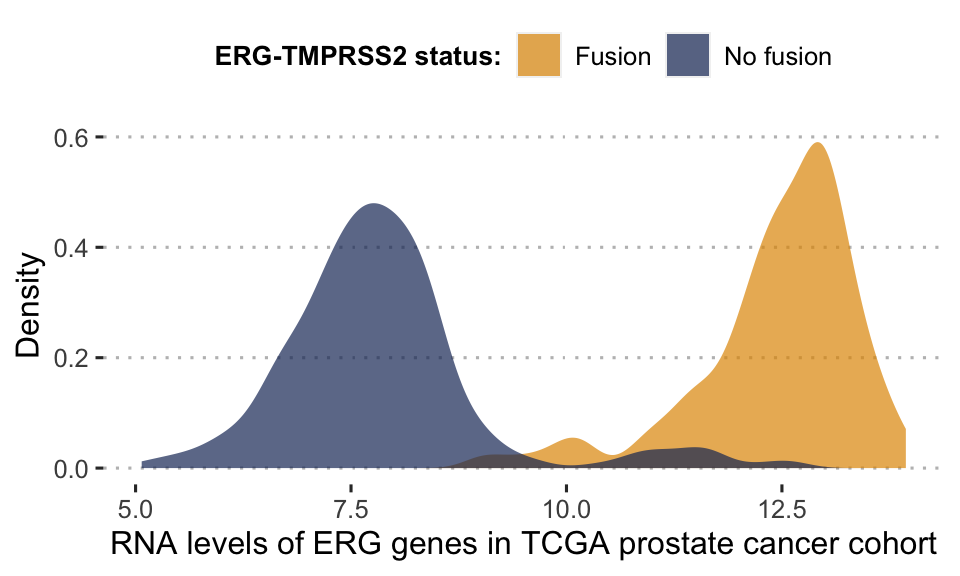
\includegraphics[width=0.6\linewidth]{05-Personalized_files/figure-latex/ERG-1} 

}

\caption[Bimodal distribution of ERG gene in TCGA prostate cancer cohort]{\textbf{Bimodal distribution of ERG gene in TCGA
prostate cancer cohort.} This bimodality is largely explained by the
fusion status of ERG gene. Patients for whom the gene has fused with
TMPRSS2 have a much higher level of RNA expression for ERG.}\label{fig:ERG}
\end{figure}






One of the assumptions of our analysis is that the interpretation of
continuous data can only be relative and not absolute. It is indeed
difficult to define an absolute threshold of RNA level at which a gene
will be considered as activated. This may depend on contexts,
technologies or even the way in which the data have been processed. On
the other hand, it is possible to estimate that a gene is over-expressed
for a patient compared to a cohort of interest. In contrast, the effect
of a mutation can be estimated more independently. Thus, the
\textbf{continuous data will be normalized for the whole cohort
studied}, for each gene individually. In order to retain biological
information as much as possible, distribution patterns are identified
and normalized in different ways (Figure \ref{fig:logical-processing}).
We will illustrate the process by taking the example of the expression
data expressed with continuous RNA levels. Beforehand, genes with no
variation in expression level or too many missing values are discarded
from the analysis. Then, we seek to identify first the genes that have a
\textbf{bimodal} distribution. Indeed, these naturally fit into a binary
formalism and this bimodality often has an underlying biological
explanation. As an example, in the TCGA prostate cancer cohort (used in
section \ref{prostate-model}), a gene called ERG has a bimodal
distribution when looking at RNA levels in all patients. This
distribution is almost entirely explained by an underlying genetic
alteration that is the fusion of the ERG gene with the TMPRSS2 gene
promoter (Figure \ref{fig:ERG}), which is very common in this cancer
\citep{tomlins2005recurrent}. In the data we identify bimodal patterns
based on three distinct criteria: \textbf{Hartigan's dip test of
unimodality, Bimodality Index (BI) and kurtosis}. The dip test measures
multi-modality in a sample using the maximum difference between
empirical distribution and the best unimodal distribution, i.e., the one
that minimizes this maximum difference \citep{hartigan1985dip}. Values
below \(0.05\) indicate a significant multi-modality. In PROFILE, this
dip statistic is computed using the R package \emph{diptest}. The
Bimodality Index (BI) evaluates the ability to fit two distinct Gaussian
components with equal variance \citep{wang2009bimodality}. Once the best
2-Gaussian fit is determined, along with the respective means \(\mu_1\)
and \(\mu_2\) and common variance \(\sigma\), the standardized distance
\(\delta\) between the two populations is given by

\[\delta = \dfrac{|\mu_1-\mu_2|}{\sigma}\]

and the BI is defined by

\[BI=[p(1-p)]^{1/2}\delta\]

where \(p\) is the proportion of observations in the first component. In
PROFILE, BI is computed using the R package \emph{mclust}. Finally, the
kurtosis method corresponds to a descriptor of the shape of the
distribution, of its tailedness, or non-Gaussianity. A negative kurtosis
distribution, especially, defines platykurtic (flattened) distributions,
and potentially bimodal distributions. It has been proposed as a tool to
identify small outliers subgroups or major subdivisions
\citep{teschendorff2006pack}. In our case, we focus on negative kurtosis
distributions to rule out non-relevant bimodal distributions composed of
a major mode and a very small outliers' group or a single outlier.
Although Dip test, BI and negative kurtosis criteria emerge as similar
tools in the sense that they select genes whose values can be clustered
in two distinct groups of comparable size, we choose to combine them in
order to correct their respective limits and increase the robustness of
our method. For that, we consider that \textbf{all three conditions (Dip
test, Bimodality Index and kurtosis) must be fulfilled in order for a
gene to be considered as bimodal}. The thresholds of each test are
inspired by those advocated in the papers presenting the tools
individually. Dip test is a statistical test to which the classical
\(0.05\) threshold has been chosen. In the article describing BI,
authors explored a cut-off range between 1.1 and 1.5 and we chose
\(1.5\) for the present work. Regarding kurtosis, the usual cut-off is
\(0\), but since this criterion does not directly target bimodality,
this criterion has been relaxed to \(K < 1\). Several examples of the
relative differences and complementarities between these criteria can be
seen in Figure \ref{fig:bimodality}.

\begin{figure}

{\centering 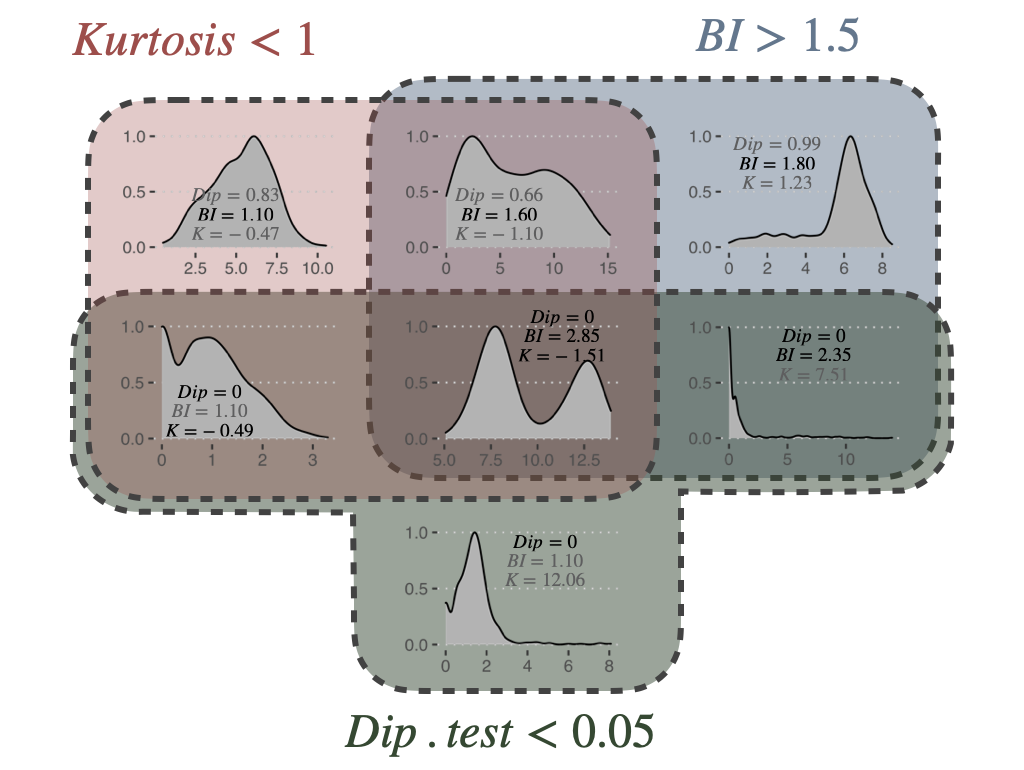
\includegraphics[width=0.8\linewidth]{fig/bimodality} 

}

\caption[Bimodality criteria and their combinations]{\textbf{Bimodality criteria and their
combinations.} Examples of gene expression distributions for the
different combinations of bimodality criteria: Dip test, Bimodality
Index (BI) and kurtosis (K). Plots are organized in a Venn diagram.}\label{fig:bimodality}
\end{figure}






Non-bimodal genes are further classified as unimodal or zero-inflated
distributions, looking at the position of the distribution density peak
(Figure \ref{fig:logical-processing}A). Then, based on this three
category classification of genes, a \textbf{pattern-preserving
normalization} can be performed, as summarized in Figure
\ref{fig:logical-processing}B. For a bimodal gene \(i\), a 2-component
Gaussian mixture model is fitted using \emph{mclust} R package resulting
in a lower mode \(M_{i,0}\) and an upper mode \(M_{i,1}\). Denoting
\(X_{i,j}\) the expression value for gene \(i\) and sample \(j\),
\(X_{i,j}\) has a probability to belong to \(M_{i,0}\) or \(M_{i,1}\)
such as \(P[X_{i,j} \in M_{i,0}]+P[X_{i,j} \in M_{i,1}]=1\). For these
bimodal genes, the normalization processing is defined as:

\[X_{i,j}^{norm}=P[X_{i,j}] \in M_{i,1}\]

For unimodal distributions, we transform data through a sigmoid function
in order to maintain the most common pattern which is unimodal and
nearly-symmetric:

\[X_{i, j}^{norm}=\dfrac{1}{1+e^{-\lambda(X_{i, j}-median(X_{i}))}}\]

Since the slope of the function depends on \(\lambda\), we adapt it to
the dispersion of initial data in order to maintain a significant
dispersion in \([0, 1]\) interval: more dispersed unimodal distributions
are mapped with a gentle slope, peaked distributions with a steep one.
We map the median absolute deviation
\(MAD(X_{i})=median(|X_{i}-median(X_i)|)\) on both sides of the median
respectively to \(0.25\) and \(0.75\) to ensure a minimal dispersion of
the mapping. Thus, the proposed mapping results in:

\[\lambda=\dfrac{log(3)}{MAD(X_i)}\]

Last, zero-inflated distributions are transformed by linear
normalization of the initial distribution:

\[X_{i, j}^{norm}=\dfrac{X_{i, j}-min(X_{i})}{max(X_{i}-min(X_{i}))}\]

The transformation is applied to data between 1st and 99th quantiles to
be more robust to outliers. Values outside this range are respectively
assigned to \(0\) and \(1\). All the categoriation of distributions and
the subsequent normalizations are summarized in Figure
\ref{fig:logical-processing}. With the help of the categories described
here, it is also possible to binarize the continuous data quite simply.
This binarization is required for some methods of network inference or
logical modeling but will not be used in the examples presented beloww.
Readers may refer to \citet{beal2019personalization} for more details.

\begin{figure}

{\centering 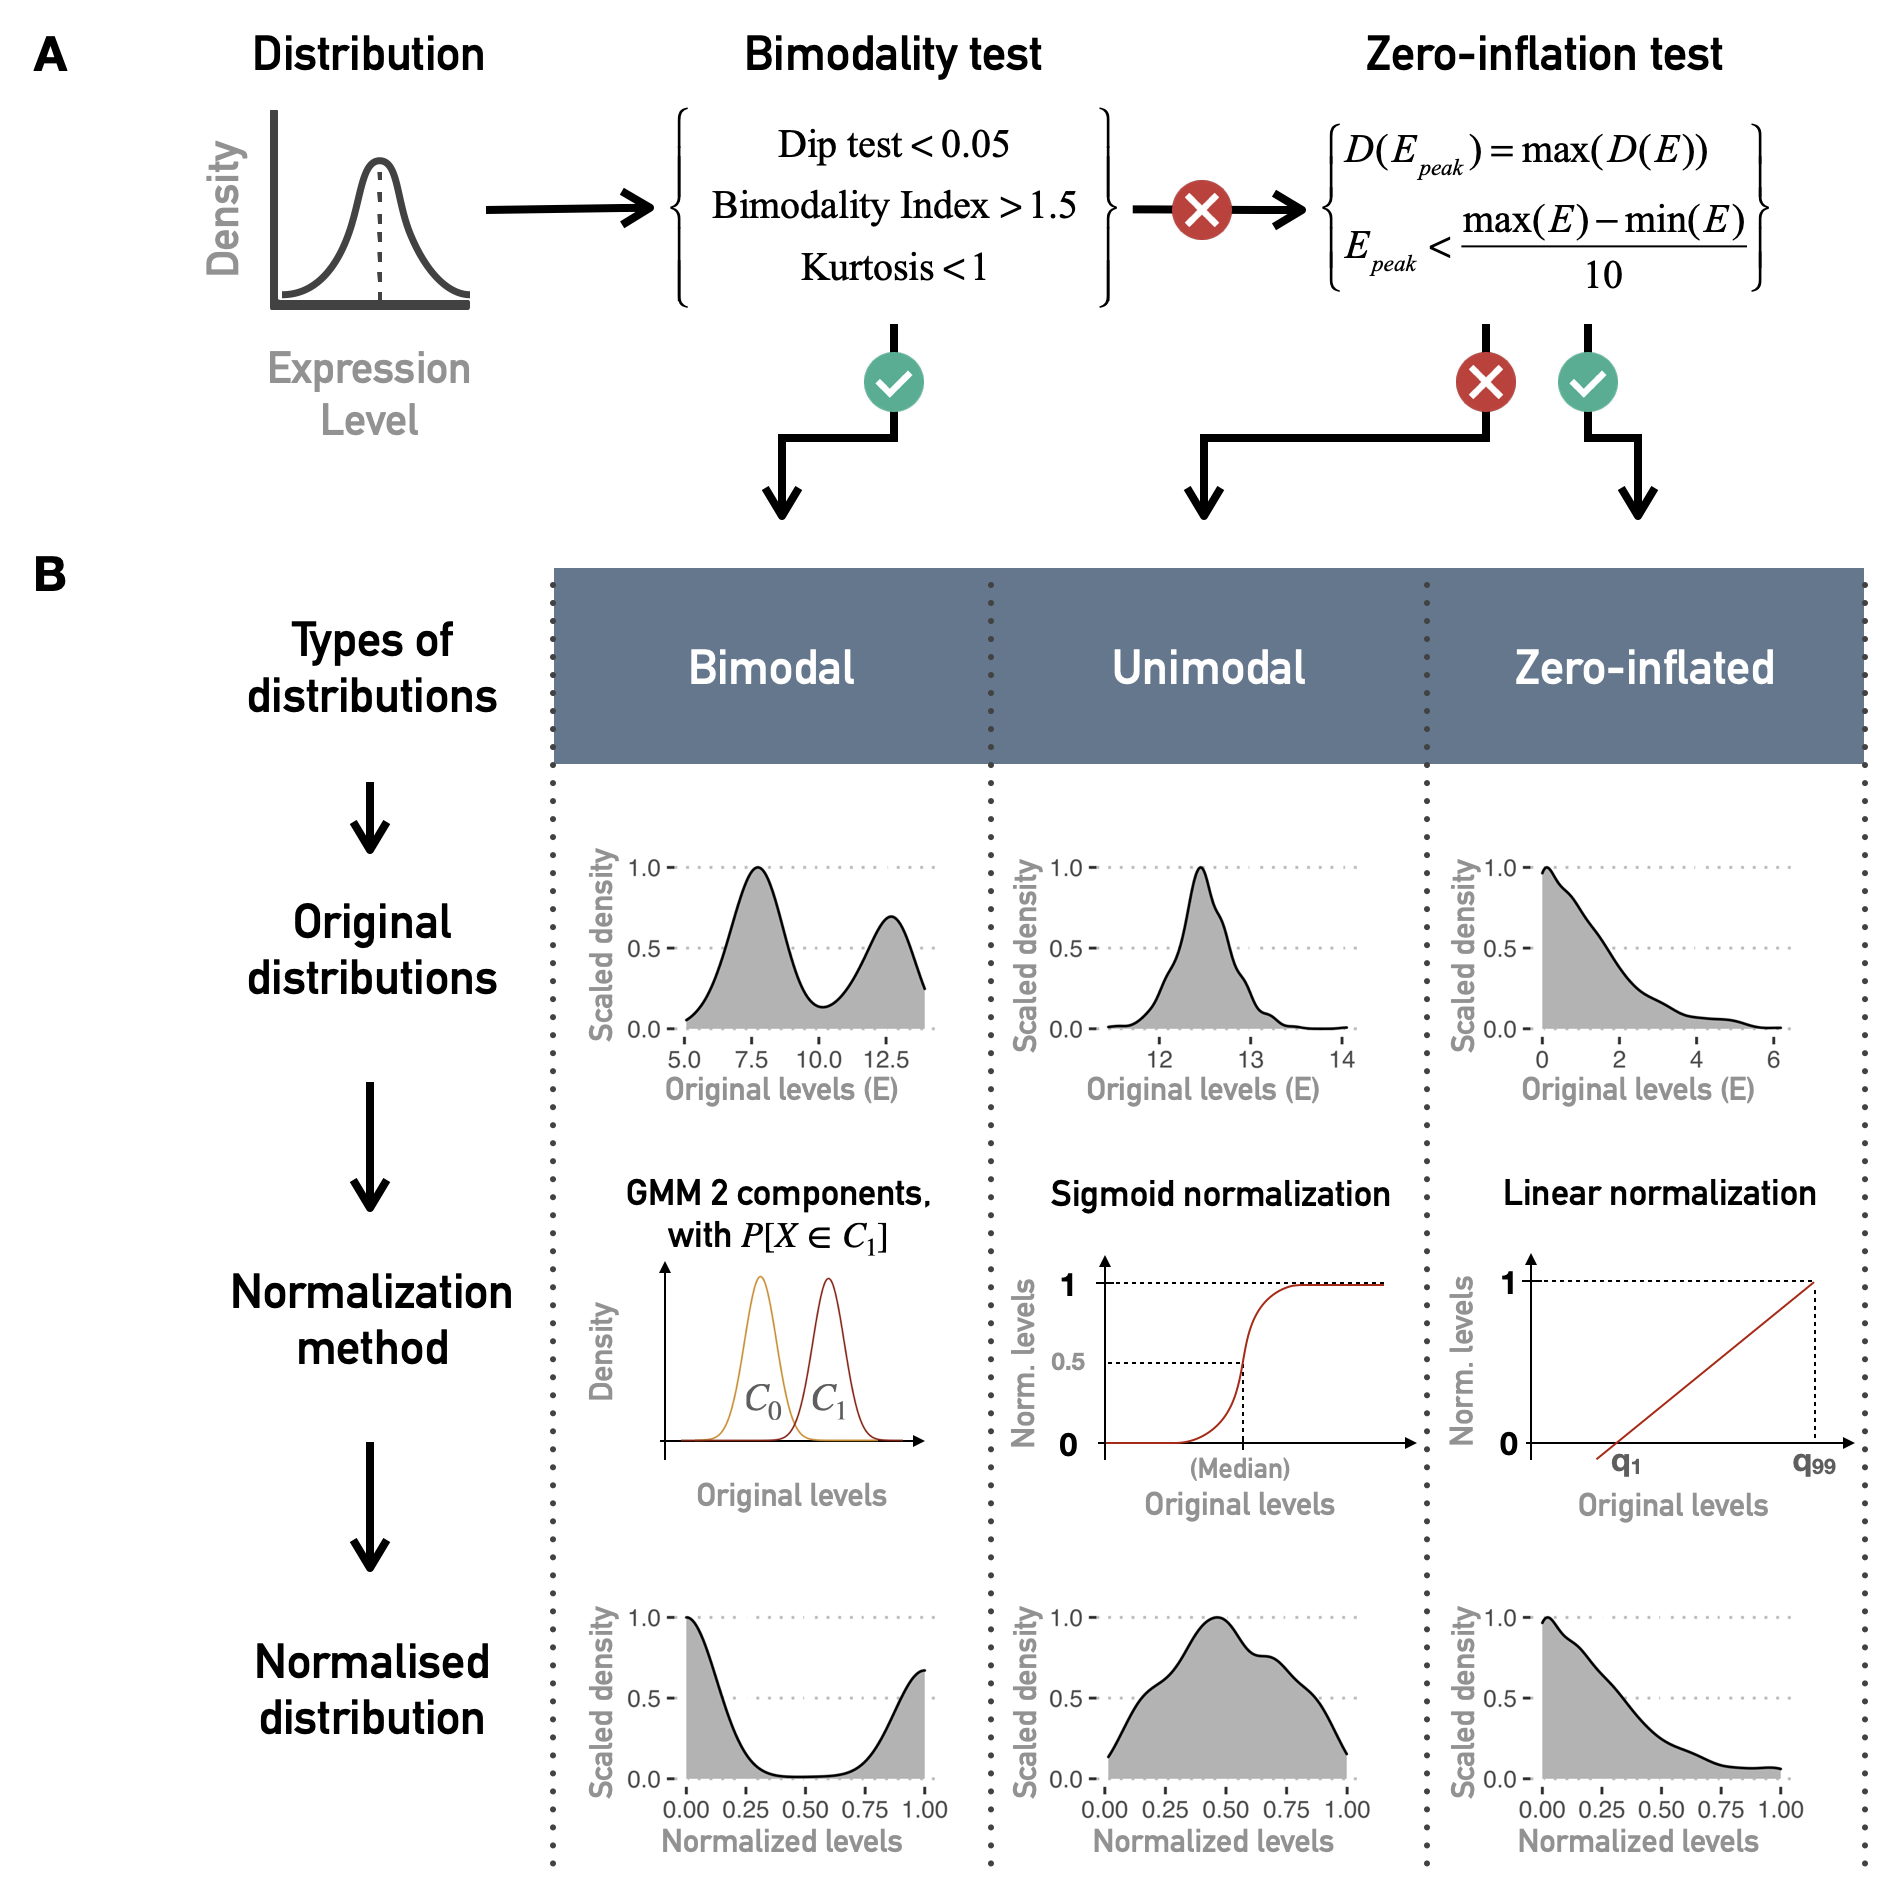
\includegraphics[width=0.8\linewidth]{fig/logical-processing} 

}

\caption[Normalization of continuous data for logical modeling]{\textbf{Normalization of continuous
data for logical modeling.} (A) Combinations of tests and criteria to
classify distributions of continuous data (such as gene expression for
one gene and all patients) as bimodal, unimodal or zero-inflated. (B)
Normalization methods for each kind of distribution.}\label{fig:logical-processing}
\end{figure}







\subsection{Personalizing logical models with patient
data}\label{personalizing-logical-models-with-patient-data}

It is now possible to redefine more precisely the ways of integrating
data into a logical model defined with MaBoSS, as sketched at the
beginning of the previous section. \textbf{Personalization is defined
here as the specification of a logical model with data from a given
patient}: each patient has a personalized model tailored to his/her
data, so that all personalized models are different specifications of
the same logical model, using data from different patients (Figure
\ref{fig:PROFILE-abstract}). Based on MaBoSS formalism and the processed
patient data, there are several possibilities to personalize a generic
logical model with patient data. One possibility to have
patient-specific models is to force the value of the variables
corresponding to the altered genes in a given patient, i.e.,
constraining some model nodes to an inactive (\(0\)) or active (\(1\))
state (Figure \ref{fig:logical-personalization}A). In order to constrain
a node to \(0\) (resp. \(1\)), the initial value of the node is set to
\(0\) (resp. \(1\)) and \(k_{0\rightarrow 1}\) (resp.
\(k_{1\rightarrow 0}\)) to \(0\) to force the node to maintain its
initially defined state. For instance, the effect of a TP53 inactivating
mutation can be modeled by setting the node \emph{p53} in the model and
its initial condition to \(0\) and ignoring the logical rule of p53
variable. Because of the type of data used, this personalization method
is referred to as \textbf{discrete personalization}. It has also been
called \emph{strict node variants} in \citet{beal2019personalization}
because this data integration overwrites the logical rules.

\begin{figure}

{\centering 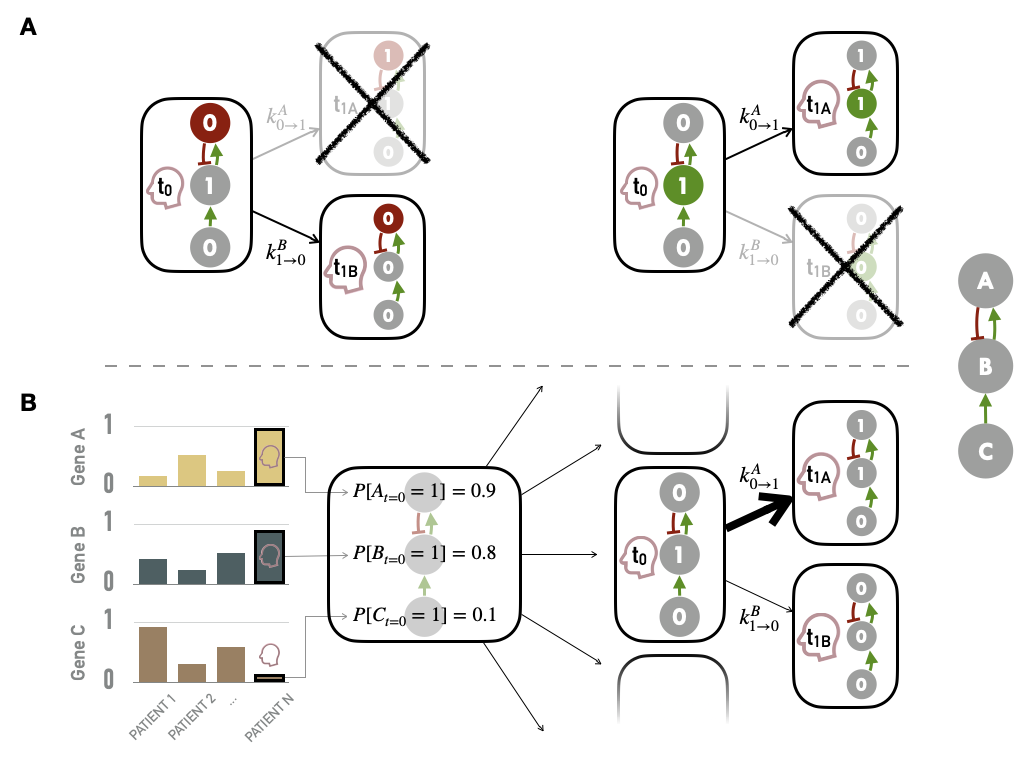
\includegraphics[width=0.9\linewidth]{fig/logical-personalization} 

}

\caption[Methods for personalization of logical models]{\textbf{Methods for
personalization of logical models.} (A) Personalization with discrete
data, such as mutations, with some nodes forced to \(0\) based on loss
of function alteration (left) or \(1\) based on gain of
function/constitutive activation (right). (B) Personalization with
continuous data used to define the initial conditions of nodes and to
influence the transitions rates and the subsequent probabilities of
transition in asynchronous updates.}\label{fig:logical-personalization}
\end{figure}










Another possible strategy is to modify the initial conditions of the
variables of the altered genes according to the results of the
normalization (i.e., the probability of initial activation for one node
among the thousands of stochastic trajectories). These initial
conditions can capture different environmental and genetic conditions.
Nevertheless, in the course of the simulation, these variables will be
prone to be updated depending on their logical rules. Finally, as MaBoSS
uses Gillespie algorithm to explore the STG, data can be mapped to the
transition rates of this algorithm. In the simplest case, all transition
rates of the model are set to \(1\), meaning that all possible
transitions are equally probable. Alternatively, it is possible to
separate the speed of processes by setting the transition rates to
different values to account for what is known about the reactions: more
probable reactions will have a larger transition rate than less probable
reactions \citep{stoll2012continuous}. For this, different orders of
magnitude for these values can be used. They are set according to the
activation status of the node (derived from normalized values) and an
amplification factor \(F\), designed to generate a higher relative
difference in the transition rates, and are therefore defined for each
node \(i\) and sample \(j\):

\[k^{0\rightarrow1}_{i,j}=F^{2(X^{norm}_{i,j}-0.5)}\]
\[k^{1\rightarrow0}_{i,j}=\dfrac{1}{k^{0\rightarrow1}_{i,j}}\] Thus, if
a gene has a value of \(1\) based on its RNA profile,
\(k_{0\rightarrow1}\) (resp. \(k_{1\rightarrow0}\)) will be \(10^2\)
(resp. \(10^{-2}\)) with an amplification factor of \(100\). This
amplification factor is therefore a hyper-parameter of the method. Very
low values of \(F\) will have no impact while higher values will make
some transitions almost impossible and the method will then approach the
discrete personalization described above. Some quantitative
illustrations of the influence of \(F\) are provided in
\citet{beal2019personalization}. The integration of continuous data
through the initial conditions of the nodes and the transition rates are
combined to form a second personalization method called
\textbf{continuous personalization} and described in Figure
\ref{fig:logical-personalization}B. This method has also been called
\emph{soft node variants} to emphasize its difference with
discrete/strict personalization: it may influence the trajectories in
the solution state space leading to a change in probabilities of the
resulting stable state but it does not overwrite the logical rules. To
illustrate a little more explicitly the impact of continuous
personalization, if a given node has a normalized value of \(0.8\) after
data processing (based on proteins levels for instance), it will be
initialized as \(1\) in 80\% of the stochastic trajectories, its
transition rate \(k_{0\rightarrow1}\) will be increased (favoring its
activation) and its transition rate \(k_{1\rightarrow0}\) will be
decreased (hampering its inactivation). These changes increase the
probability that this node will remain in an activated state close to
the one inferred from the patient's data, while maintaining the validity
of its logical rule. Thus, continuous personalization appears as a
smoother way to shape logical models' simulations based on patient data.

In summary, different types of data can be used, with different
integration methods. Note that it is quite natural to use genetic
alterations (mutations, CNA) to specify definitive changes in models
(such as those of discrete personalization) since this corresponds to
biological reality: a mutation cannot be undone or reversed. Conversely,
continuous alterations in expression or phosphorylation are subject to
modification and regulation, thus justifying their interpretation in a
less strong and definitive way (such as continuous personalization).
Finally, it follows from these definitions that there are different
strategies for personalizing a logical model since discrete and
continuous personalizations can each use different types of data; and
moreover, these two strategies can be combined. \textbf{Except otherwise
stated, mutations (resp. RNA or protein) will always be integrated using
discrete (resp. continuous) personalization and the joint integration of
both types of data will therefore combine both methods.} The relative
merits of the different personalization strategies will be discussed
below.

\section{An integration tool for high-dimensional
data?}\label{an-integration-tool-for-high-dimensional-data}

Once the method has been defined, it is imperative to study its validity
and possible limitations. This comes down to answering the question: do
personalized models capture a biological reality, and in our case do
they discriminate between different types of cancer?

\subsection{Biological relevance in cell lines}\label{PROFILE-CL}

These questions can be addressed using cell line data. Using the logical
model of cancer pathways from \citet{fumia2013boolean}, it is possible
to study the 663 cell lines from different types of tumors by
integrating their processed omics profiles to the generic logical model
to obtain as many personalized models. If we focus on the read-out of
\emph{Proliferation}, one of the easiest to interpret, there are several
ways to study its relevance. For each cell line and each personalization
strategy (and corresponding data type) we can define a personalized
model and derive the asymptotic value the \emph{Proliferation} node,
called \emph{Proliferation} score. This score is therefore \emph{a
priori} different for all cell lines that present a different molecular
profile. For the whole population of cell lines, this score can be
confronted with other markers of proliferation such as the levels of
Ki67 \citep{miller2018ki67}, here replaced as an example by the RNA
levels of the corresponding MKI67 gene. It can then be observed that the
simulated \emph{Proliferation} indicator, derived from the personalized
models, correlates positively with the biomarker, but only when RNA has
been used in the personalization (Figure \ref{fig:PROFILE-CL}A). The
\textbf{correlation makes qualitative sense, but the heterogeneity
appears to be very large and most of the variability is not captured by
the models}. This heterogeneity is also visible by focusing on some
types of cancer (Figure \ref{fig:PROFILE-CL}B). Thus this kind of
comparison only validates the models' ability to retrieve a RNA
biomarker (not used in personalization) when they themselves integrate
other RNA data. It is also consistent that scores from models
personalized with mutations only have less uniform distributions due to
the discrete nature of the data and the many identical profiles: many
cell lines are not distinguishable by mutations only.

\begin{figure}

{\centering 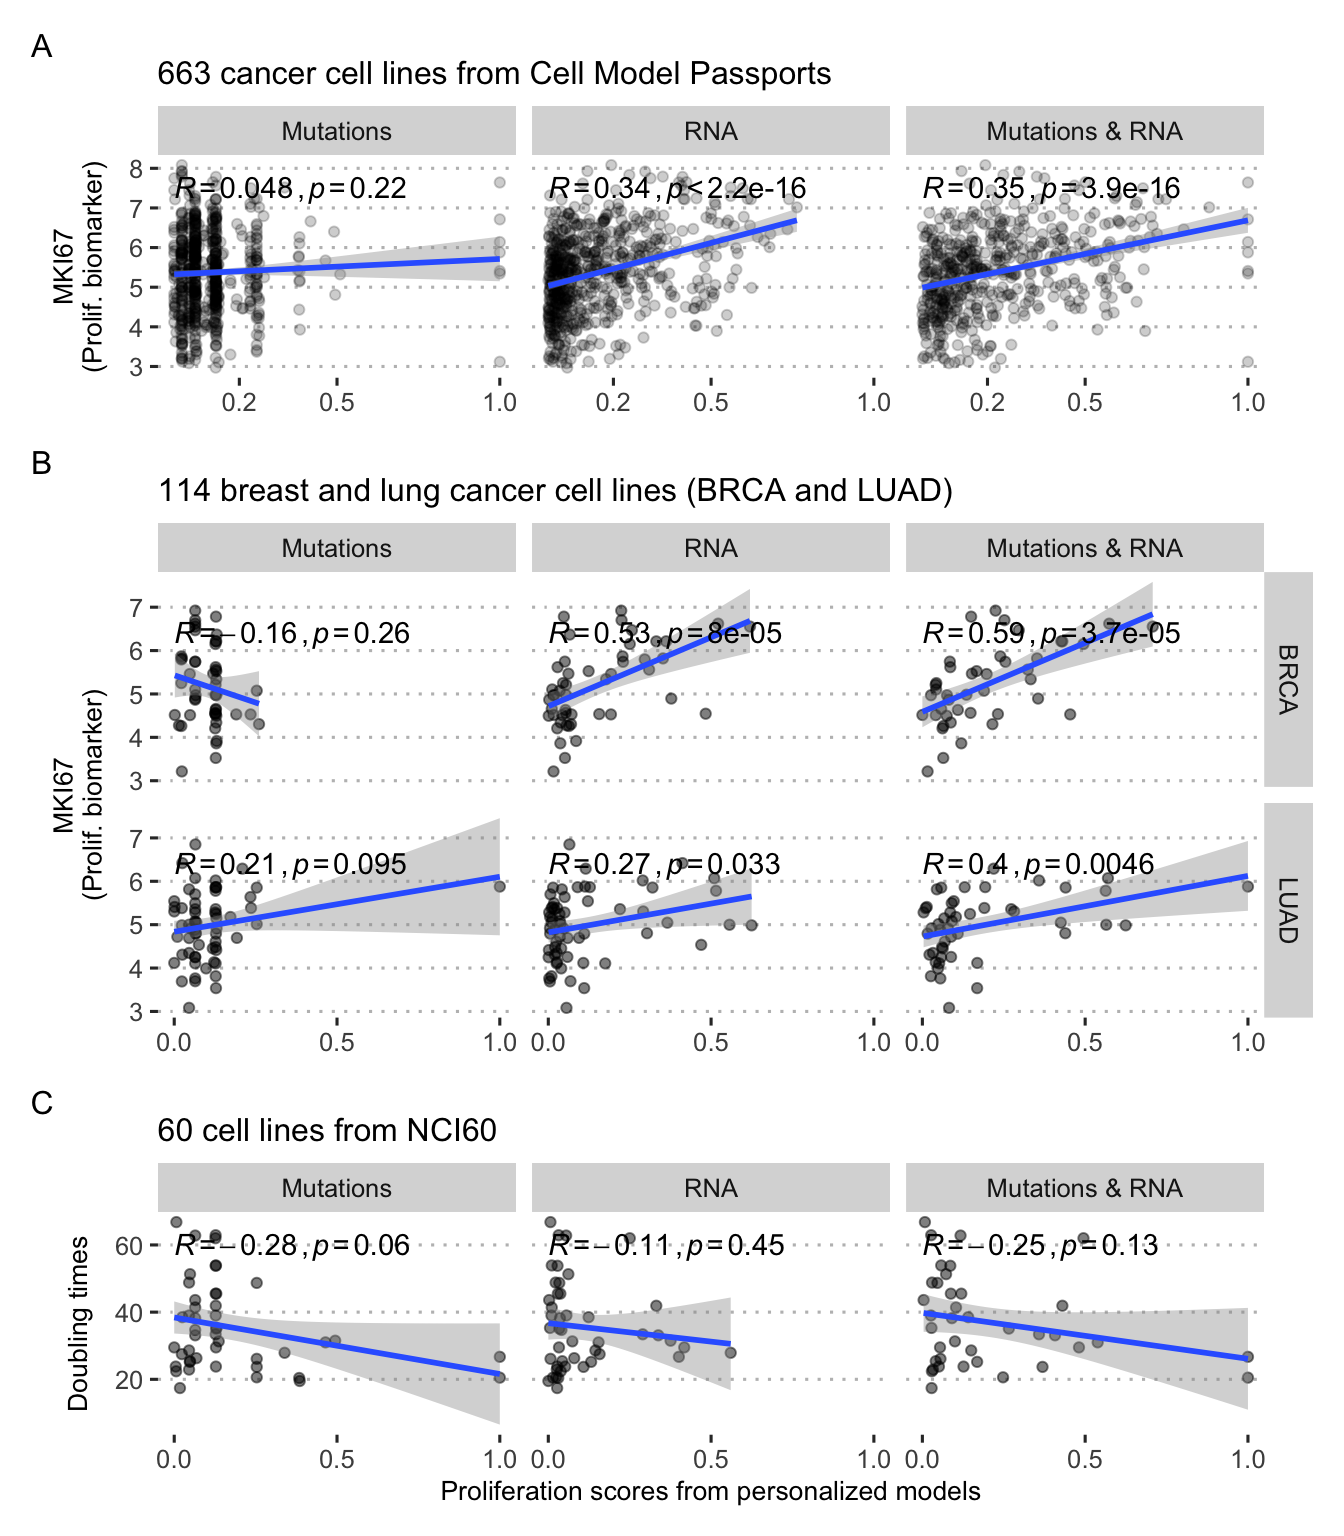
\includegraphics[width=0.9\linewidth]{05-Personalized_files/figure-latex/PROFILE-CL-1} 

}

\caption[Validation of personalized *Proliferation* scores in cell lines]{\textbf{Validation of personalized
\emph{Proliferation} scores in cell lines.} (A) Comparison with MKI67
proliferation biomarker for all cancer cell lines. (B) Same with breast
(BRCA) and lung (LUAD) cancer only. (C) Comparison with doubling times
in a subset of 60 cell lines.}\label{fig:PROFILE-CL}
\end{figure}







It is possible to go one step further by comparing these personalized
\emph{Proliferation} scores with the doubling time of the cell lines,
i.e., the time it takes for the cell line population to double. A cell
line described as proliferative (high \emph{Proliferation} score) should
thus have a low doubling time. This can be observed qualitatively by
using a subgroup of cell lines for which this information is available
(Figure \ref{fig:PROFILE-CL}C). These correlations are not significant
and once again summarize a large heterogeneity. Predicting doubling
times is, however, a rather difficult task with poor accuracies, even
with the help of more flexible machine learning low
\citep{kurilov2020assessment}.

\subsection{Validation with patient
data}\label{validation-with-patient-data}

\begin{figure}

{\centering 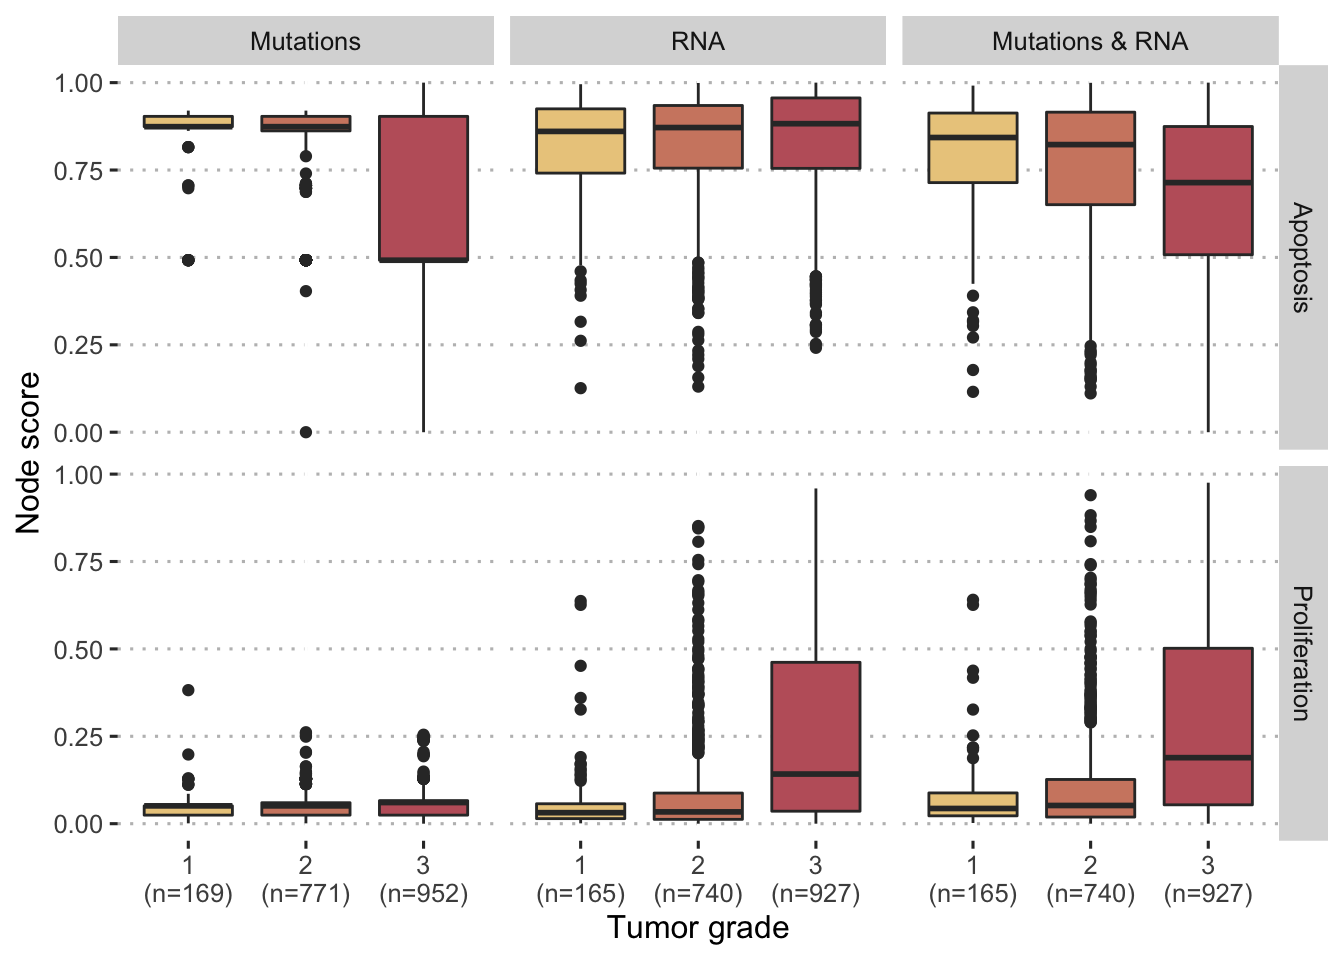
\includegraphics[width=0.9\linewidth]{05-Personalized_files/figure-latex/PROFILE-METABRIC-Grade-1} 

}

\caption[Prognostic value of *Proliferation* scores for breast cancer patients in METABRIC cohort]{\textbf{Comparaison of personalized
scores with tumor grades for breast cancer patients in METABRIC cohort.}
Comparisons are provided for different personalization strategies (with
mutations and/or RNA) and two different model nodes
(\emph{Proliferation} and \emph{Apoptosis}).}\label{fig:PROFILE-METABRIC-Grade}
\end{figure}







Patient data can as well be used to reproduce analyses of the same type
as those previously performed with the MKI67 biomarker, as was done in
\citet{beal2019personalization}, but we focus here on the more clinical
applications of the personalized mechanistic models. By analogy with the
validations proposed for other mechanistic models
\citep{fey2015signaling}, it is also possible to evaluate the
\textbf{prognostic value of personalized logical models on patient
data}. For example, when studying breast cancer patients in the METABRIC
cohort, \emph{Proliferation} and \emph{Apoptosis} scores differ
according to tumor grade. The more advanced tumors (grade 3) are
associated with higher \emph{Proliferation} scores and lower
\emph{Apoptosis} scores (Figure \ref{fig:PROFILE-METABRIC-Grade}). This
is in line with the natural interpretation that could be given since
proliferation is by definition a sign of cancer progression while
apoptosis, a programmed death of defective cells, is on the contrary a
protective mechanism. While these trends are monotonous and clearly
significant for the third strategy using both mutations and RNA
(\(p<10^{-12}\) with Jonckheere--Terpstra test for ordered differences
among classes, for both nodes), this is not the case when the two types
of data are used separately: mutations (resp. RNA) are not sufficient to
personalize \emph{Proliferation} (resp. \emph{Apoptosis}) scores in a
meaningful way. The personalisation method therefore seems to be able to
combine discrete and continuous data in such a way that some of the
biological information is preserved.

\begin{figure}

{\centering 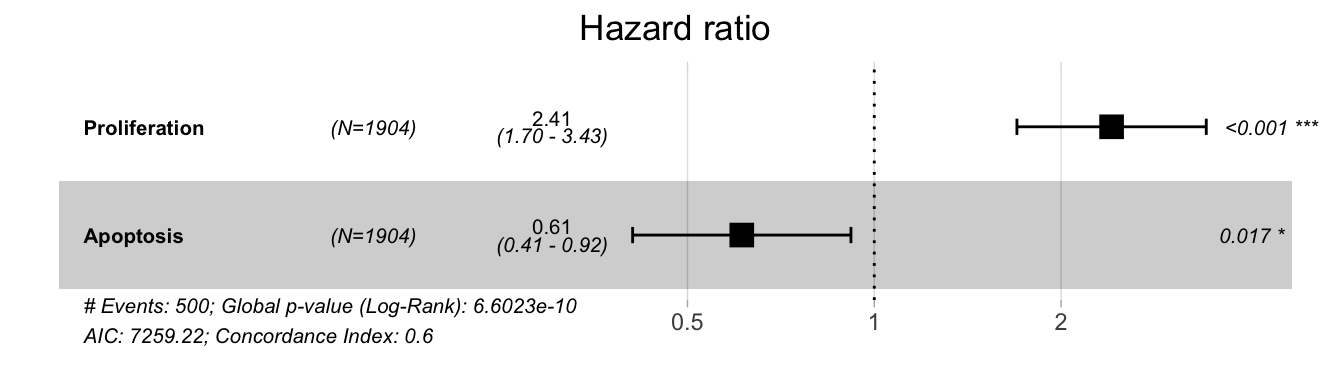
\includegraphics[width=0.9\linewidth]{05-Personalized_files/figure-latex/PROFILE-METABRIC-Cox-1} 

}

\caption[Hazard ratios for *Proliferation* and *Apoptosis* in a survival Cox model in METABRIC cohort]{\textbf{Hazard ratios for
\emph{Proliferation} and \emph{Apoptosis} in a survival Cox model in
METABRIC cohort.} Higher \emph{Proliferation} (resp. \emph{Apoptosis})
scores correspond to higher (resp. lower) probabilities of death.}\label{fig:PROFILE-METABRIC-Cox}
\end{figure}






This comparison to clinical data can be extended to \textbf{patient
survival data} in the same cohort. If we focus on the strategy
integrating both mutations and RNA, we observe that in a Cox model of
survival, \emph{Proliferation} is significantly associated with a higher
risk of event while \emph{Apoptosis} is associated with a lower risk,
which is again consistent (Figure \ref{fig:PROFILE-METABRIC-Cox}). In a
more schematic and visual way, it is possible to transform these
continuous \emph{Proliferation} and \emph{Apoptosis} scores into binary
indicators (using medians) and observe their impact on survival, as has
been done in previously mentioned studies
\citep{fey2015signaling, salvucci2019system}. We then observe the same
behaviour for the two personalized scores (Figure
\ref{fig:PROFILE-METABRIC-Survival}A and B). Interestingly, if we
combine the indicators to create groups that are expected to be of very
bad prognosis (high \emph{Proliferation}, low \emph{Apoptosis}) or of
very good prognosis (low \emph{Proliferation}, high \emph{Apoptosis}),
we further discriminate patients and confirm the qualitatively
meaningful interpretation of the personalized scores. It should be noted
that the clinical validations presented here remain voluntarily simple
and quite close to those proposed in similar articles. Discussions and
statistical developments will be proposed in Part III.

\begin{figure}

{\centering 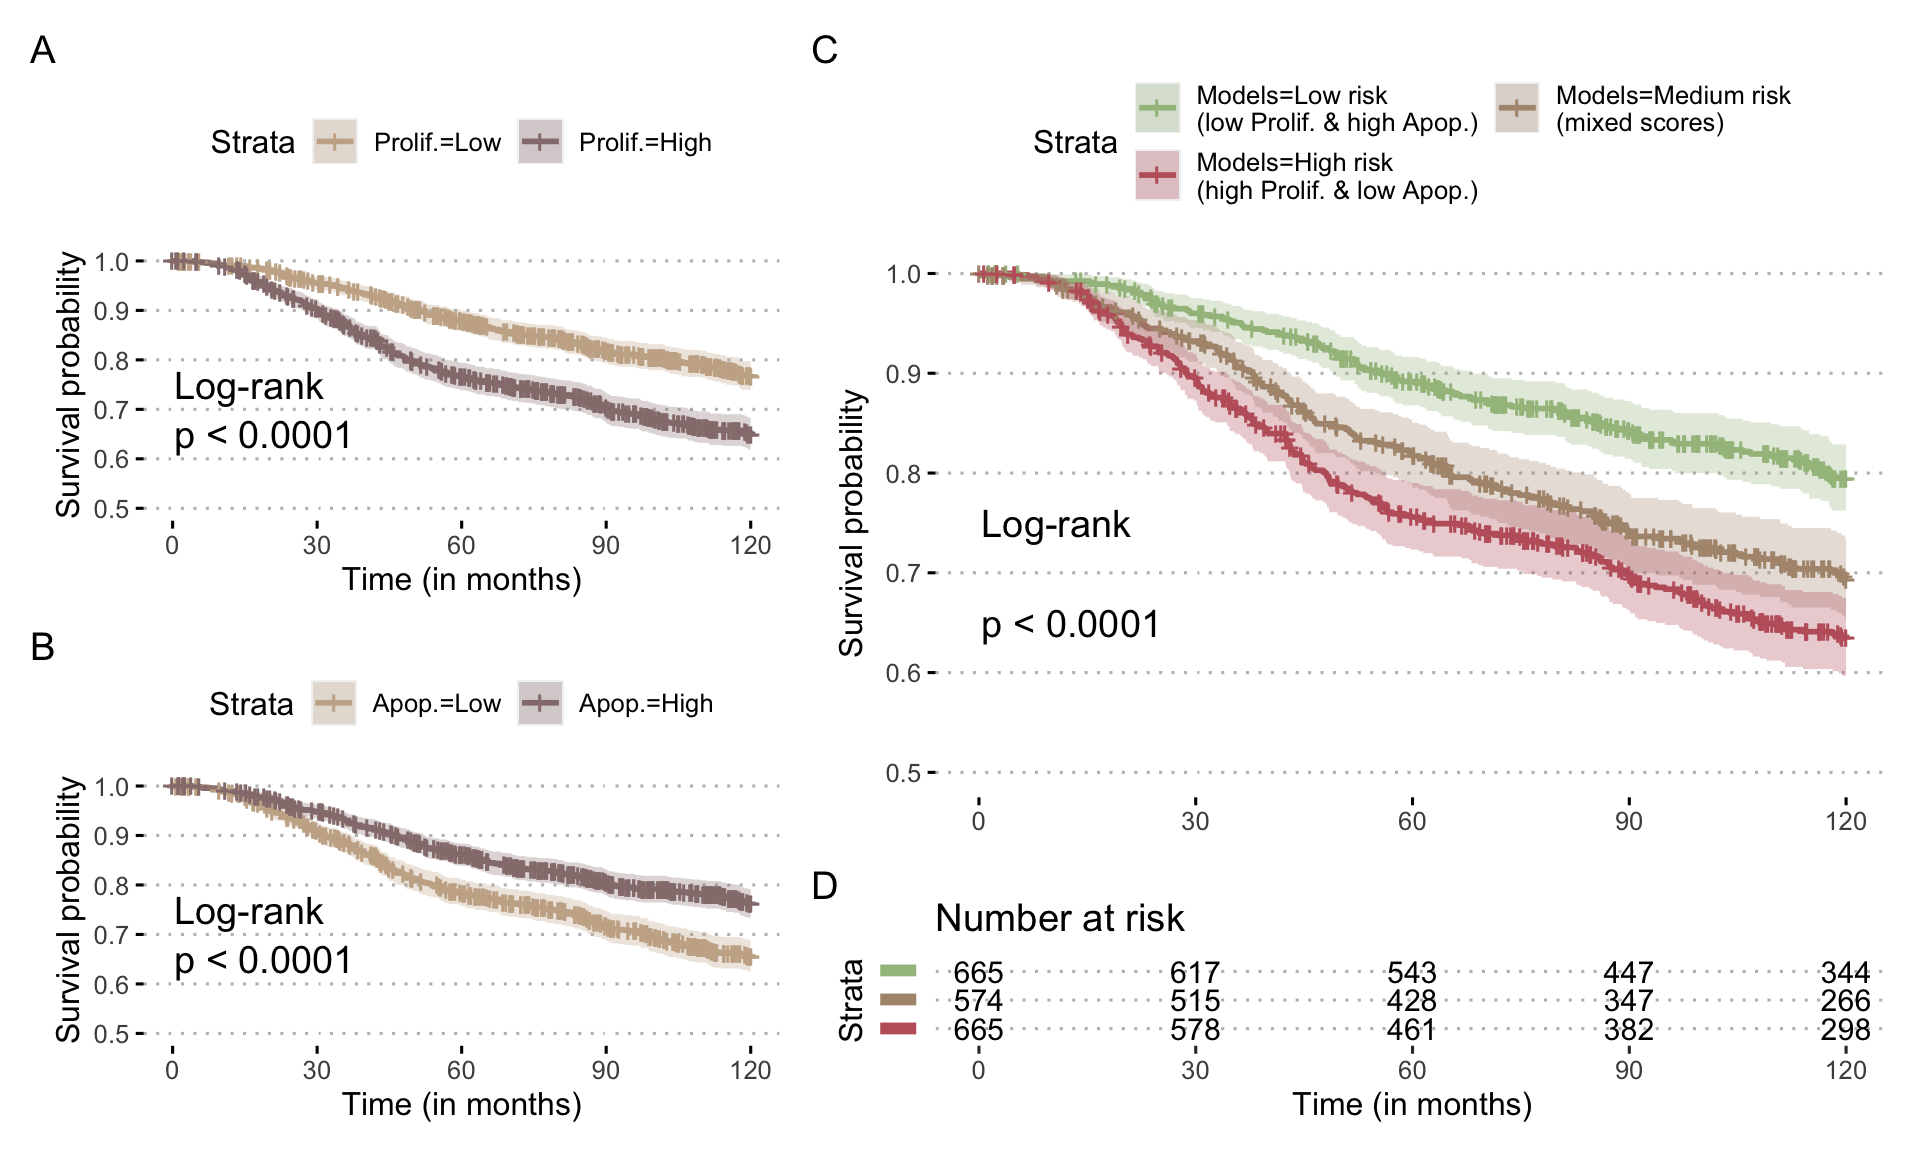
\includegraphics[width=0.9\linewidth]{05-Personalized_files/figure-latex/PROFILE-METABRIC-Survival-1} 

}

\caption[Prognostic value of *Proliferation* scores for breast cancer patients in METABRIC cohort]{\textbf{Prognostic value of
\emph{Proliferation} scores for breast cancer patients in METABRIC
cohort.} (A) Survival curve for overall survival stratified with
\emph{Proliferation} scores from personalized models integrating
mutations and RNA; scores have binarized based on median and survival
censored at 120 months. (B) Same with \emph{Apoptosis} scores. (C)
Survival curve stratified with combinations of \emph{Proliferation} and
\emph{Apoptosis} scores, based on the same thresholds, and the
corresponding number of patients at risk (D).}\label{fig:PROFILE-METABRIC-Survival}
\end{figure}











\subsection{Perspectives}\label{perspectives}

In summary, this kind of application of personalized models allows the
\textbf{integration of quite heterogeneous and moderately dimensional
biological data in a constrained framework} that orders the
relationships between variables and guides interpretations. Comparison
with external biological or clinical data then makes it possible to
verify the absence of major contradictions in the definition of the
model. However, the interest of these mechanistic approaches in this
type of task appears as quite moderate compared to statistical models.
The qualitative aspect is not necessarily compensated here by the
integration of knowledge into the structure of the model, especially in
examples that use an extremely broad logical model, which has not been
specifically designed for the problems to which it is applied. It is
then necessary to study the application of these personalized models to
more suitable problems, in which the explicitly mechanistic nature of
the models can be exploited.

\chapter{Personalized logical models to study an interpret drug
response}\label{personalized-logical-models-to-study-an-interpret-drug-response}

\epigraph{"Il serait excellent que tout médecin ait la possibilité d'expérimenter un grand nombre de médicaments sur lui-même. Sa compréhension de leurs effets en serait tout autre."}{Mikhail Bulgakov (Morphine, 1927)}

\initial{H}istorically, all mechanistic models of molecular networks,
and logical models in particular, have been widely used to study
response to treatments
\citep{flobak2015discovery, jastrzebski2018integrative}. Indeed,
biological entities, many of which are prospective therapeutic targets,
are explicitly represented in the model, making it possible to simulate
their inhibition. This is what will be presented in this chapter using
the personalized logical models described above. Can they be used to
study the response of biological systems to perturbations, in this case
the response of cell lines to gene or protein inhibitions? Compared to
the numerous statistical models designed to predict the sensitivity of
cell lines to treatements, what information do these personalized
mechanistic models provide?

\BeginKnitrBlock{summarybox}
\subsubsection*{Publications}\label{publications-2}
\addcontentsline{toc}{subsubsection}{Publications}

This chapter extends the method presented in the previous chapter to
investigate drug response with personalized logical models. The first
application to cell lines of all cancer types was presented orally at
ISMB2020 in Basel but is not published.

The example about BRAF in melanomas and colorectal cancers is under
review and the corresponding pre-print is available as
\citet{beal2020personalized}. In this joint work, only the construction
of the generic logical model was mostly carried out by collaborators and
will therefore be described more succinctly.

Finally, the work on prostate cancer presented in a third section will
be submitted soon. It is also a joint work, in which my participation
focused on the application of the PROFILE method.
\EndKnitrBlock{summarybox}

\section{One step further with drugs}\label{one-step-further-with-drugs}

One of the main clinical consequences of the underlying molecular
complexity of cancers is the divergent response to treatment, even for a
priori similar tumors. In the light of high-throughput sequencing data,
the mechanisms governing these responses are somewhat better understood,
for patients and especially for model organisms such as cell lines
{[}\citet{heiser2012subtype}; garnett2012systematic{]}. But beyond a few
simple cases, the diversity of response biomarkers once again calls for
\textbf{holistic approaches} to unravel the underlying mechanisms.

\subsection{Modeling response to cancer
treatments}\label{modeling-response-to-cancer-treatments}

To study these observed differences in drug response in various cancers,
some approaches based on mathematical modeling were developed to explore
the complexity of differential drug sensitivities. A number of
\textbf{machine learning-based methods for predicting sensitivities}
have been proposed \citep{costello2014community}, either without
particular constraints or with varying degrees of prior knowledge; but
they do not necessarily provide a mechanistic understanding of the
response. Some other approaches focused on the description of the
processes that might influence the response by integrating knowledge of
the signaling pathways and their mechanisms and translated it into a
mathematical model
\citep{eduati2017drug, jastrzebski2018integrative, frohlich2018efficient}.
The first step of this approach implies the construction of a network
recapitulating knowledge of the interactions between selected biological
entities (driver genes but also key genes of signaling pathways),
extracted from the literature or from public pathway databases, or
directly inferred from data \citep{verny2017learning}. This static
representation of the mechanisms is then translated into a dynamical
mathematical model with the goal to not only understand the observed
differences \citep{jastrzebski2018integrative} but also to predict means
to revert unexpected behaviours.

One way to address issues related to patient response to treatments is
to \textbf{fit these mechanistic models to the available data}, and to
train them on high-throughput cell-line specific perturbation data
\citep{eduati2017drug, jastrzebski2018integrative, klinger2013network}.
These mechanistic models are then easier to interpret with regard to the
main drivers of drug response. They also enable the \emph{in silico}
simulations of new designs such as combinations of drugs not present in
the initial training data \citep{frohlich2018efficient}. However, these
mechanistic models contain many parameters that need to be fitted or
extracted from the literature. Some parsimonious mathematical formalisms
have been developed to make up for the absence of either rich
perturbation data to train the models or fully quantified kinetic or
molecular data to derive the parameters directly from literature. One of
these approaches is the logical modeling, which uses discrete variables
governed by logical rules. Its explicit syntax facilitates the
interpretation of mechanisms and drug response
\citep{zanudo2017network, iorio2016landscape} and despite its
simplicity, semi-quantitative analyses have already been performed on
complex systems including drug response studies
\citep{knijnenburg2016logic, eduati2020patient}.

\subsection{An application of personalized logical
models}\label{an-application-of-personalized-logical-models}

But logical formalism has also shown its relevance regarding drug
response in cases where the model is not automatically trained on data
but simply constructed from literature or pathway databases and where
biological experiments focus on a particular cell line
\citep{flobak2015discovery}. The study is then restricted to one cell
line only from which some data and parameters have been experimentally
inferred. Using the PROFILE method, it is possible to generate
personalized logical models associated with different cell lines and
then use them to study the response to treatment. \textbf{Since the
models are not trained with perturbation data but simply
specified/constrained by interpreting the molecular profiles, it is
possible to do this with a rather limited amount of data}.

\begin{figure}

{\centering 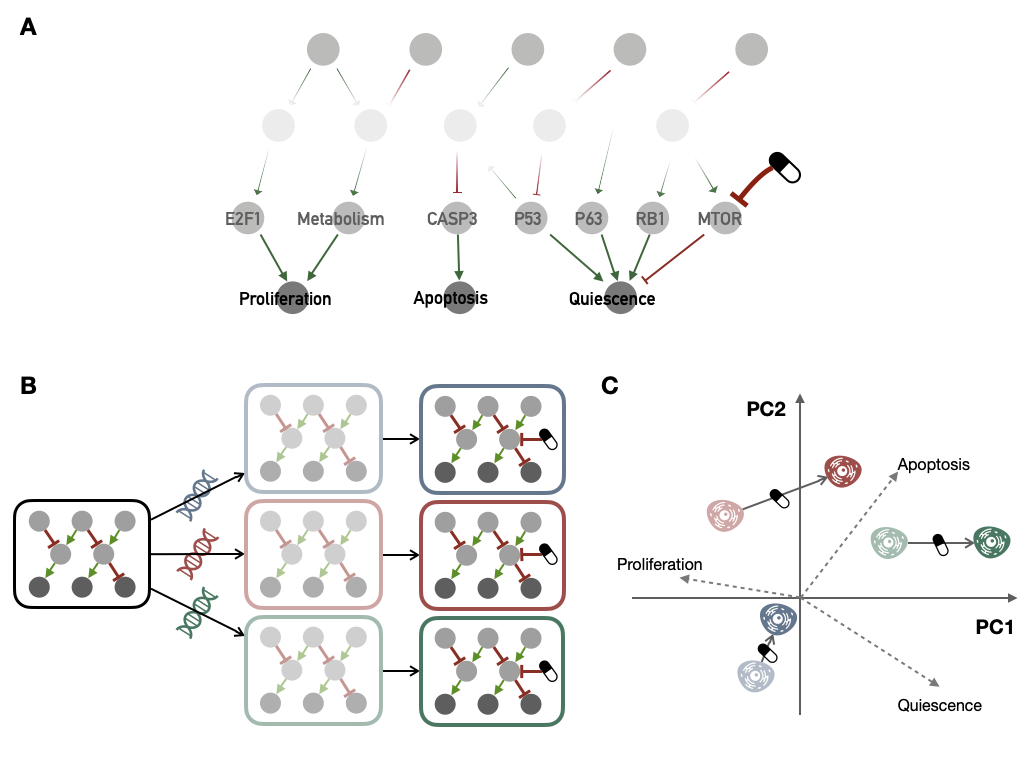
\includegraphics[width=0.9\linewidth]{fig/PROFILE-drug} 

}

\caption[Bimodality criteria and their combinations]{\textbf{Schematic extension of
PROFILE-personalized logical models to drug investigation.} (A)
Schematic representation of a logical model of cancer molecular
networks, in particular the one described in appendix
\ref{appendix-verlingue} and used in the nexte subsection. (B)
Sequential pipeline for drug response investigation with PROFILE,
starting from a generic logical model, then transformed into several
personalized models with different molecular profiles (correspondong to
several cell lines); these models are finally simulated with a defined
drug inhibition. (C) A possible analysis of the predictions of
personalized models obtained from the generic model described in (A);
the position of the personalized models in the PCA phenotype (or
read-out) space of the model is studied as well as the impact of the
treatment on this position.}\label{fig:PROFILE-drug}
\end{figure}
















The principles are summarized in Figure \ref{fig:PROFILE-drug}. A
generic model (Figure \ref{fig:PROFILE-drug}A) is first transformed into
as many personalized models as there are cell lines with an omics
profile. These persnalized models are then simulated by adding the
effect of a given treatment (Figure \ref{fig:PROFILE-drug}B). The
treatments that can be studied are generally targeted inhibitors.
Generally speaking, one must be able to \textbf{translate the mechanism
of action of the treatment into the logical model}. The impact of more
systemic treatments such as chemotherapy or radiotherapy is more
difficult to study with these methods, in any case with most of the
logical models published to date, even if in theory, precise modelling
of the pathways associated with these treatments (such as DNA repair)
could contribute to this.

It is then possible to analyze the personalized scores for each cell
line (asyptotic values of the phenotypic read-outs of the model) with or
without the effect of treatment. If the model includes more than two
phenotypes of interest, such as the one in Figure
\ref{fig:PROFILE-drug}A, one can visualize these behaviors in the PCA
space of the personalized scores, as shown schematically in Figure
\ref{fig:PROFILE-drug}C. In this case the directions of the original
phenotype features (\emph{Proliferation}, \emph{Apoptosis},
\emph{Quiescence}) have been added in the PCA-transformed space in order
to facilitate the interpretation of positions and drug-induced
displacements. In this mock example, based on personalized models,
treatment would promote a shift from proliferative to more apoptotic or
quiescent behaviors, in particular in the red and green cell lines,
which are a priori more sensitive to the treatment.

\subsection{A pan-cancer attempt}\label{a-pan-cancer-attempt}

This versatile analysis framework was first applied during this thesis
to a \textbf{large pan-drug and pan-cancer analysis}. On the basis of
generic logical models such as those previously presented (cf appendix
\ref{appendix-fumia} and \ref{appendix-verlingue}), and in view of the
abundance of available data (across cancer tissues and drugs such as in
GDSC cell line dataset, cf appendix \ref{appendix-fumia}), there were no
theoretical obstacles to such an analysis. Although the simulations were
carried out without any problems, the analysis nevertheless proved
extremely difficult to interpret. We will highlight the various problems
encountered, propose an illustration and some perspectives that led to
the work presented in the following section.

Based on the PROFILE methodology and GDSC data, hundreds of personalized
models can be obtained, each corresponding to a cell line. For each of
these personalized models, several dozen of potential drugs have a
mechanism of action that can be mechanistically translated into the
logical model. We thus obtain \textbf{tens of thousands of
``personalized model/drug'' pairs that correspond to experimentally
evaluated drug sensitivies} (cf appendix @ref(\#appendix-GDSC) for
details). Firstly, the comparison of simulated and experimental data is
not straightforward. As the models are qualitative, it is necessary to
carry out the validation in this spirit. The idea is not to predict
sensitivity quantitatively, rather to verify their relative relevance.
In the first place, do we recover the cell lines that are most sensitive
to a given drug? With several hundred cell lines, it is difficult to
make this reflection graphically as in Figure \ref{fig:PROFILE-drug}C.
More quantitative approaches, such as correlation, would require the
\textbf{definition of a precise sensitivity proxy in personalized
models}. Should we choose the personalised \emph{Proliferation} score
obtained with drug? Or the drug-induced displacement in the mechanistic
model (the drug arrows in Figure \ref{fig:PROFILE-drug}C)? Or is a
combination of phenotypes used, if so which one? As for experimental
metrics, which ones to choose, and what interpretations do they allow?
Whatever the choice, dose-response AUC or IC50 (see details in the
appendix \ref{appendix-GDSC}), a problem arises: can the sensitivities
of a cell line to different drugs be compared? Such a comparison would
allow the most clinically interesting questions of precision medicine to
be asked: for a given molecular profile, can the model predict the best
treatment to administer? However, AUCs are comparable for different
drugs only if the concentration ranges tested are similar; and IC50s are
extrapolated, sometimes well beyond the concentrations tested.
Qualitative comparisons for a given drug therefore seem the most
meaningful, as long as a relevant proxy in personalized models can be
justified.

Aware of these difficulties, if one decides to do a correlation
analysis, for each drug, of the personalized correlation scores with
experimental sensitivities, one realizes that responses to
\textbf{certain drugs are correctly predicted when others are not
correlated at all}. But it is difficult to decide between two different
interpretations: does this mean that correctly predicted drugs are well
modelled and others are not? Or does it mean that some correlations
appear to be better by chance because so many drugs have been modeled? A
case study can be illustrated more precisely with the example shown in
Figure \ref{fig:PROFILE-PCA}. In order to simplify the analysis
presented schematically in Figure \ref{fig:PROFILE-drug}C, the 663 cell
lines were averaged by cancer type (according to
\href{https://gdc.cancer.gov/resources-tcga-users/tcga-code-tables/tcga-study-abbreviations}{TCGA
denominations}) and the drug-induced shifts are all represented from the
origin in the PCA space. There is evidence that the effect of the drug
on personalized models (using only mutations) tends to make them less
proliferative and more apoptotic/quiescent (Figure
\ref{fig:PROFILE-PCA}A). This shift is strongest for those types of
cancer that are actually most sensitive to this inhibitor experimentally
(i.e.~low AUC), such as skin cutaneous melanomas (SKCM) in particular,
and colorectal (COAD/READ) or pancreatic (PAAD) cancers to a lesser
extent. The ability of personalized models to explain this difference
can be understood by a known underlying biological reality: the
prevalence of BRAF or RAS mutations in these cancers. The three
aforementioned cancers are thus very frequently mutated for one of the
two genes (Figure \ref{fig:PROFILE-PCA}B). Then, the model translates
the fact that these two genes are located just upstream of MAP2K1. It is
therefore natural that an inhibition just downstream of these important
mutations is particularly effective (Figure \ref{fig:PROFILE-PCA}C). In
a case such as this, the relevance of the model can be explained and
justified \emph{a posteriori}. This analysis is much more difficult in
the vast majority of cases, whether the correlations are apparently good
or not.

\begin{figure}

{\centering 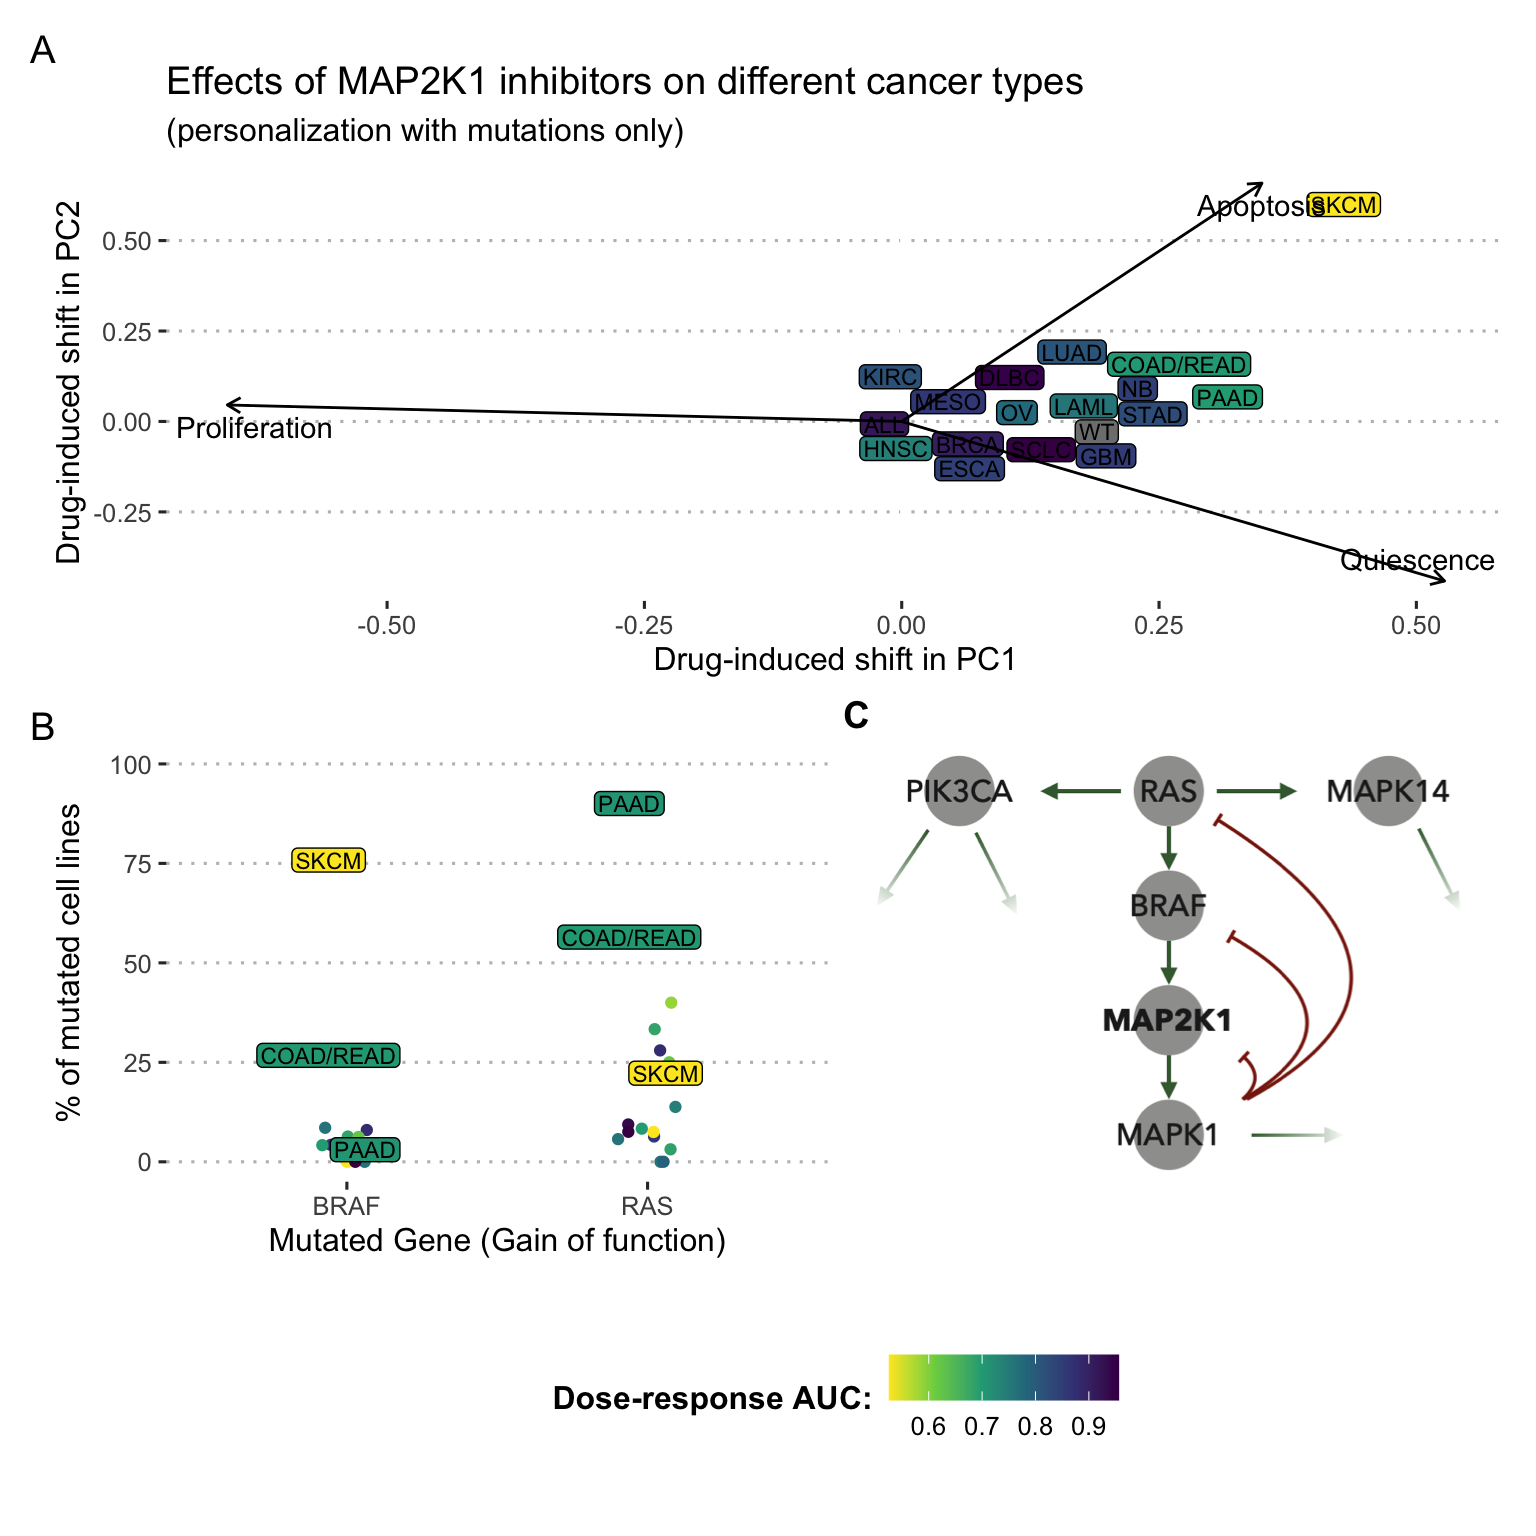
\includegraphics[width=0.9\linewidth]{06-Drugs_files/figure-latex/PROFILE-PCA-1} 

}

\caption[PROFILE-generated models and sensitivites to MAP2K1  inhibitors avergaed per cancer type]{\textbf{PROFILE-generated models and
sensitivites to MAP2K1 inhibitors avergaed per cancer type.} (A) Effects
of MAP2K1 inhibitors on personalized logical models averaged per cancer
types and represented in a normalized PCA space with super-imposed
original phenotypes. (B) Proportion of BRAF- and RAS-mutated cell lines
in some cancer types. (C) Zoom on the MAPK pathway of the logical model
used.}\label{fig:PROFILE-PCA}
\end{figure}









This example highlights a problem of scope. \textbf{The fact that the
method enables to study hundreds of cell lines and dozens of drugs does
not mean that it is relevant in each case}. The description of pathways
in the model is more or less accurate. For example, a node at the model
boundaries probably has many regulators missing. Is it then relevant to
investigate the response of personalized models to its inhibition? It is
therefore necessary to restrict the drugs studied. Similarly, even if
the logical model summarizes many important pathways, it is probably
unsuitable for certain cell lines or certain types of cancer with
different etiologies. However, it is difficult to restrict the scope of
the analysis in an unbiased way without having designed a model \emph{de
novo} for a specific purpose.

For all these reasons, it was decided to leave aside this naive,
broad-spectrum approach in favour of starting from a more specific
biological question and constructing the appropriate logical model.

\section{Case study on BRAF in melanoma and colorectal
cancers}\label{case-study-on-braf-in-melanoma-and-colorectal-cancers}

In order to address the limitations outlined in this exploratory
analysis, we propose here a pipeline based on logical modeling and able
to go from the formulation of a specific biological question to the
validation of a mathematical model on pre-clinical data, in this case a
set of cell lines, and the subsequent interpretation of potential
resistance mechanisms (Figure \ref{fig:BRAF-GA}). As before,** one of
the main points of differentiation with existing mechanistic approaches,
is that this framework does not rely on any training of parameters but
only on the automatic integration and interpretation of omics
features**.

\begin{figure}

{\centering 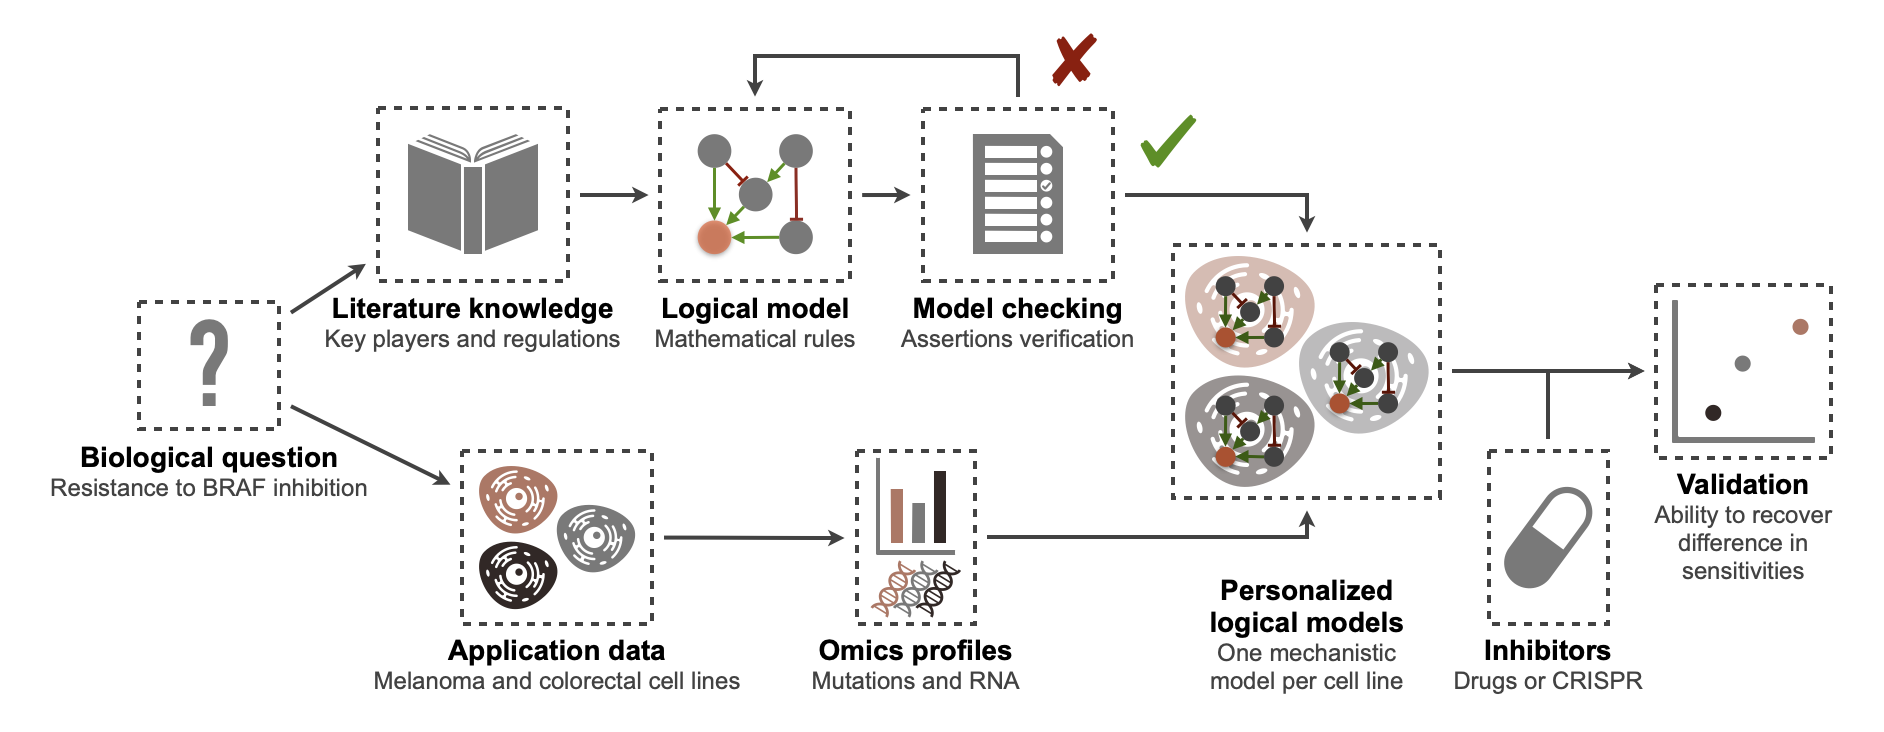
\includegraphics[width=0.9\linewidth]{fig/BRAF-GA} 

}

\caption[BRAF modelling flowchart: from a biological question to validated personalized logical models]{\textbf{BRAF modelling flowchart: from a
biological question to validated personalized logical models.}}\label{fig:BRAF-GA}
\end{figure}




\subsection{Biological and clinical
context}\label{biological-and-clinical-context}

The construction of a mathematical model must be based first and
foremost on a precise and specific biological problem, at the origin of
the design of the model. Here, we choose to explore the different
responses to treatments in diverse cancers that bear the same mutation.
A well-studied example of these variations is the BRAF mutation and
especially its V600E substitution. BRAF is mutated in 40 to 70\% of
melanoma tumors and in 10\% of colorectal tumors, each time composed
almost entirely of V600E mutations \citep{cantwell2011brafv600e}. In
spite of these similarities, \textbf{BRAF inhibition treatments have
experienced opposite results with improved survival in patients with
melanoma \citep{chapman2011improved} and significant resistance in
colorectal cancers \citep{kopetz2010plx4032}}, suggesting drastic
mechanistic differences. Some subsequent studies have proposed
context-based molecular explanations, often highlighting surrounding
genes or signalling pathways, such as a feedback activation of EGFR
\citep{prahallad2012unresponsiveness} or other mechanisms
{[}\citet{poulikakos2011raf}; sun2014reversible{]}. These various
findings support the need for an integrative mechanistic model able to
formalize and explain more systematically the differences in drug
sensitivities depending on the molecular context. The purpose of the
study we propose here is not to provide a comprehensive molecular
description of the response but to verify that the existence and
functionality of the suggested feedback loops around the signalling
pathway in which BRAF is involved \citep{prahallad2012unresponsiveness}
may be a first hint towards these differences. For a more thorough study
of these cancers, we refer to other works
\citep{eduati2017drug, baur2020connecting, cho2016attractor}.

\subsection{A logical model centred on
BRAF}\label{a-logical-model-centred-on-braf}

A logical model summarizing the main molecular interactions at work in
colorectal cancers and melanomas is thus built from the literature and
completed with databases. As previously mentioned, the objective is to
understand whether it is possible to model and explain differences in
responses to BRAF inhibition in melanoma and colorectal cancer patients
using the same regulatory network. \textbf{The fact that the two cancers
share the same network but differ from the alterations and expression of
their genes constitutes our prior hypothesis}. The focus of this model
is put on two important signaling pathways involved in the mechanisms of
resistance to BRAF inhibition which are the ERK1/2 MAPK and PI3K/AKT
pathways \citep{ursem2018emerging, rossi2019drug}. The generic network
presented in Figure \ref{fig:BRAF-model} recapitulates the known
interactions between the biological entities of the network that was
first built from the literature, and then verified and completed with
potential missing connections using SIGNOR database
\citep{perfetto2016signor}. More details and references about the model
can be found in appendix \ref{appendix-pantolini}. All in all, the
logical model formalizes the knowledge compiled from different sources
and highlights the role of SOX10, FOXD3, CRAF, PI3K, PTEN and of EGFR in
resistance to anti-BRAF treatments.

\begin{figure}

{\centering 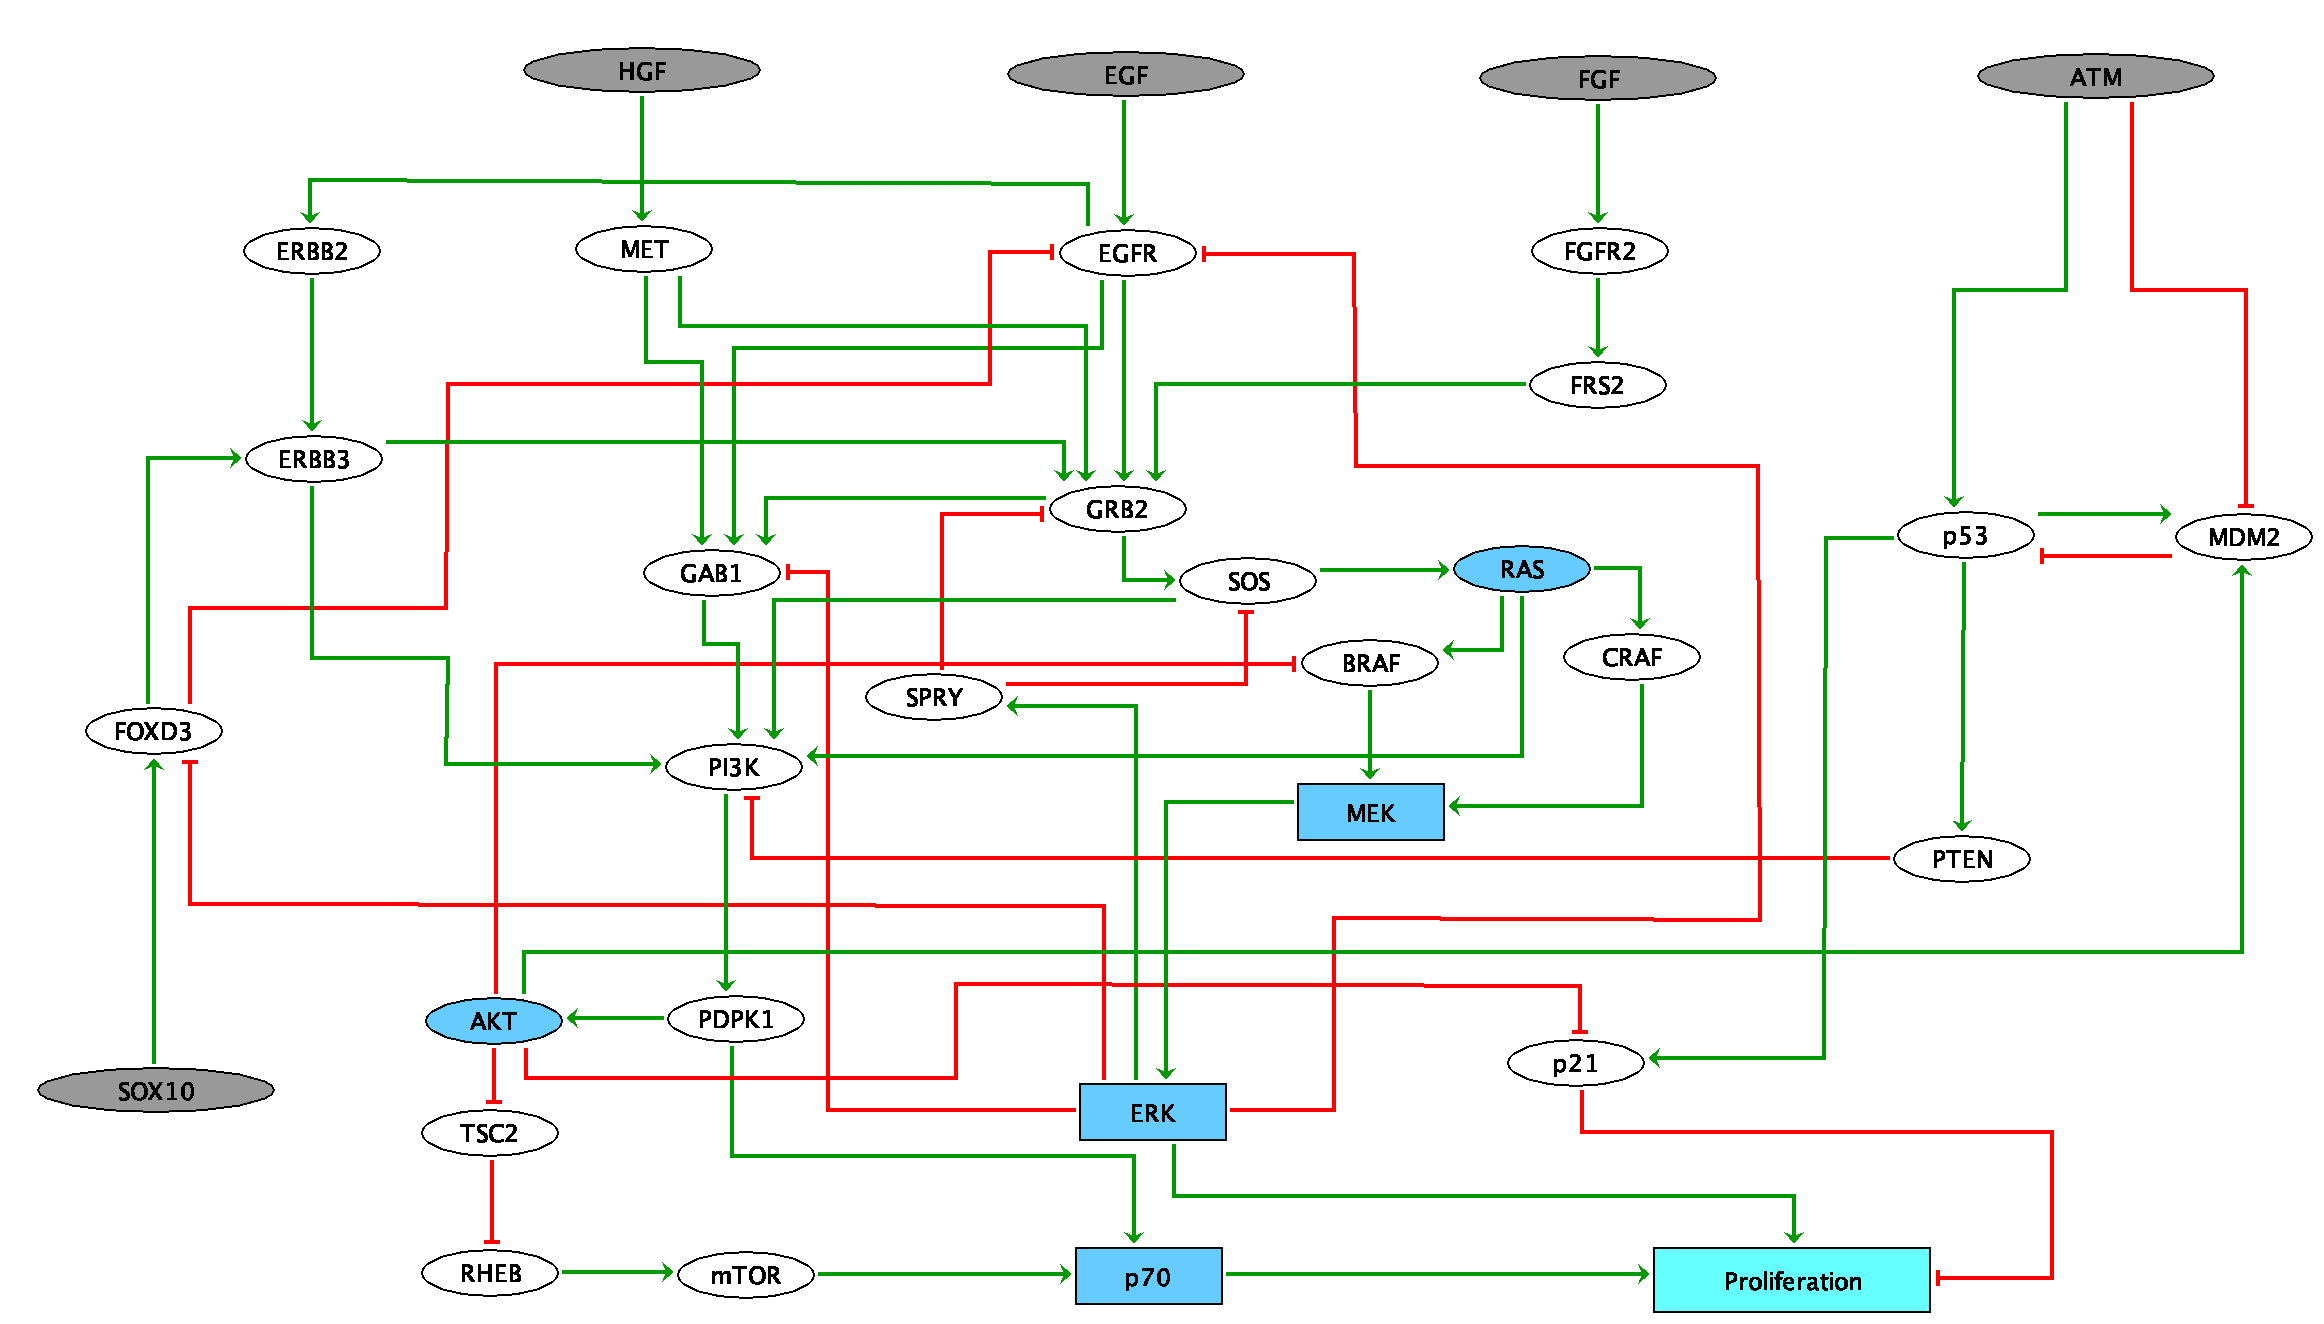
\includegraphics[width=0.9\linewidth]{fig/BRAF-model} 

}

\caption[Bimodality criteria and their combinations]{\textbf{Logical model of signaling pathways
around BRAF in colorectal andmelanoma cancers.} Grey nodes represent
input nodes, which may correspond to the environmental conditions.
Square nodes represent multi-valued variable (MEK, ERK, p70 and
Proliferation). Dark blue nodes accounts for families (several
genes/entities for one node). Light blue node represents the phenotypic
read-out of the model, i.e. \emph{Proliferation}.}\label{fig:BRAF-model}
\end{figure}









Once the structure of the model was defined, and before moving on to its
personalization, its consistency with the literature was checked using a
\textbf{model-checking procedure}. Indeed, due to the complexity of the
system, properly taking into account the interactions between entities
does not automatically guarantee that the model will reproduce certain
dynamic behaviours. An example of a biological assertion may be the
reactivation of the MAPK (mitogen-activated protein kinase) pathway
through EGFR signal after BRAF inhibition in colorectal cancer
\citep{prahallad2012unresponsiveness}: it is possible to check whether a
simulation of this situation with the model gives the same result or
not. Because there are many such assertions and because it is useful to
verify them as the model is built, automatic model-checking tools have
been defined, based on the MaBoSS syntax and inspired by the python
unittest library. More details are provided in
\citet{beal2020personalized} and in a corresponding
\href{https://github.com/sysbio-curie/MaBoSS_test}{GitHub repository}.
The list of biological assertions used to validate the model is detailed
in the appendix \ref{appendix-pantolini}.

\subsection{Cell lines data}\label{cell-lines-data}

The omics profiles of colorectal and melanoma cell lines are downloaded
from Cell Model Passports portal \citep{van2019cell}. 64 colorectal
cancer (CRC) cell lines and 65 cutaneaous melanoma (CM) cell lines are
listed in the database, with at least mutation or RNA-seq data (59 CM
and 53 CRC with both mutations and RNA-seq data). These omics profiles
are used to generate cell-line-specific logical models as described in
PROFILE method (Figure \ref{fig:PROFILE-abstract}). The prevalence of
mutations and their combination for the two types of cancer can be seen
in Figure \ref{fig:BRAF-GDSC}A and is consistent with the clinical
situation described above with melanomas more frequently BRAF-mutated
and colorectal cancers more frequently RAS-mutated.

\begin{figure}

{\centering 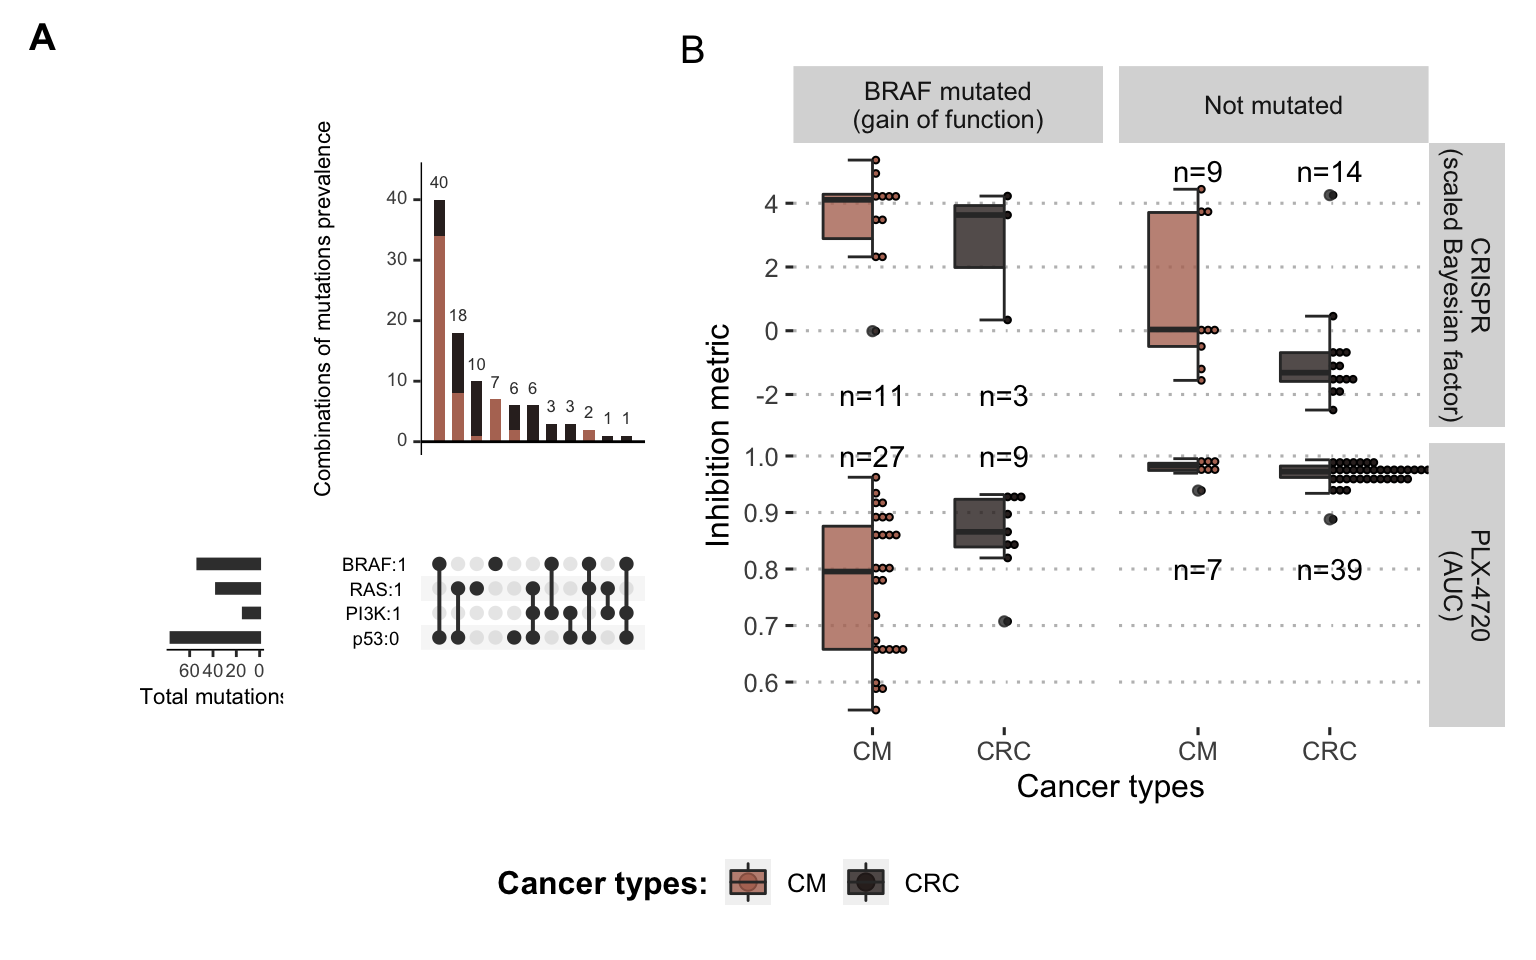
\includegraphics[width=0.95\linewidth]{06-Drugs_files/figure-latex/BRAF-GDSC-1} 

}

\caption[Descriptive analysis of cell lines for melanomas and colorectal cancers]{\textbf{Descriptive analysis of cell lines for
melanomas and colorectal cancers.} (A) Number of cell lines for the four
most frequently mutated genes and their combinations (plot from UpSetR
package \citep{conway2017upsetr}). (B) Differential sensitivities to
BRAF inhibition by the drug PLX-4720 (lower panel) or by CRISPR
inhibition (upper panel), depending on BRAF mutational status and cancer
type. Numbers of cell lines in eache category are indicated. Note that
high sensitivities correspond to low AUC and high scaled Bayesian
factors.}\label{fig:BRAF-GDSC}
\end{figure}











In order to validate the relevance of personalized models to explain
differential sensitivities to drugs, some experimental screening
datasets are used. \textbf{Drug screening data} are downloaded from the
Genomics of Drug Sensitivity in Cancer (GDSC) dataset
\citep{yang2012genomics} which includes two BRAF inhibitors: PLX-4720
and Dabrafenib. The cell lines are treated with increasing concentration
of drugs and the viability of the cell line relative to untreated
control is measured. The dose-response relative viability curve is
fitted and then used to compute the \textbf{area under the dose-response
curve (AUC)} \citep{vis2016multilevel}. AUC is a value between \(0\) and
\(1\): values close to \(1\) mean that the relative viability has not
been decreased, and lower values correspond to increased sensitivity to
inhibitions (details in appendix \ref{appendix-GDSC}). The results
obtained with the two drugs are very strongly correlated (Pearson
correlation of \(0.91\)) and the analyses presented here will therefore
focus on only one of them, PLX-4720.

In a complementary way, some results of \textbf{CRISPR/Cas9 screening}
are also downloaded from Cell Model Passports. This technology, which is
described in more detail in the appendix \ref{appendix-CRISPR}, allows
targeted inhibitions of certain genes. Two different datasets from
Sanger Institute \citep{behan2019prioritization} and Broad Institute
\citep{meyers2017computational} are available. We use \textbf{scaled
Bayesian factors} to assess the effect of CRISPR targeting of genes.
These scores are computed based on the fold change distribution of sgRNA
\citep{hart2016bagel}. The highest values indicate that the targeted
gene is essential to the cell fitness. The agreement between the two
databases is good \citep{dempster2019agreement} but we choose to focus
on the Broad database, which is more balanced in terms of the relative
proportions of melanomas and colorectal cancers.

Figure \ref{fig:BRAF-GDSC}B illustrates both the relative quantities of
cell lines for which drug or CRISPR screening data are available
(depending on their BRAF status) as well as differences in sensitivity
to BRAF inhibition. The greater sensitivity of BRAF-mutated melanomas
compared to BRAF-mutated colorectal cancers is well observed for
PLX-4720. However, the overlap in the distributions requires a deeper
look into the data and a search for more precise explanations of the
differences in sensitivity, including within each type of cancer. The
finding appears to be similar for CRISPR despite a sample size that is
too small; the higher average sensitivity of melanomas even extends to
non-mutated BRAF.

\subsection{Validation of personalized models using CRISPR/Cas9 and drug
screening}\label{validation-of-personalized-models-using-crisprcas9-and-drug-screening}

The validation of personalized logical models using these screening data
is done with the following rationale. First, the models are personalized
using omics data from the cell lines. Then, two separate simulations are
performed for each personalized model: one without the inhibition, the
other by creating and activating a BRAF inhibitor to mimic the drug or
CRISPR inhibition. The ratio of the \emph{Proliferation} phenotype
obtained with inhibition and without inhibition is the proxy used to be
compared with the different screening metrics each of which is also
standardized (AUC calculated on relative viability for drugs and Bayes
factor computed from fold-changes and then scaled).

\subsubsection{Differential sensitivities to BRAF targeting explained by
personalized logical
models}\label{differential-sensitivities-to-braf-targeting-explained-by-personalized-logical-models}

Once the logical model consistency has been validated, personalized
models are generated for each cell line by integrating their interpreted
genomic features directly as model constraints or parameters.
\textbf{Sensitivities to BRAF inhibition inferred from models are then
compared to experimentally observed sensitivities} (Figure
\ref{fig:BRAF-results}). In all the following analyses, we focus on
three different personalization strategies using: only mutations as
discrete personalization (Figure \ref{fig:BRAF-results}A, upper row),
only RNA as continuous personalization (Figure \ref{fig:BRAF-results}A,
middle row) or mutations combined with RNA (Figure
\ref{fig:BRAF-results}A, lower row). These choices reflect first of all
the following \emph{a priori}: mutations are much more drastic and
permanent changes than RNA, whose expression levels are more subject to
fluctuation and regulation. The objective is also to answer the
following questions: What type of data is most likely to explain the
differences in responses? Is it relevant to combine them? Figure
\ref{fig:BRAF-results} shows an example of the type of analyses possible
with personalized models, zooming in more and more on the details from
panel A to panel C.

\begin{figure}

{\centering 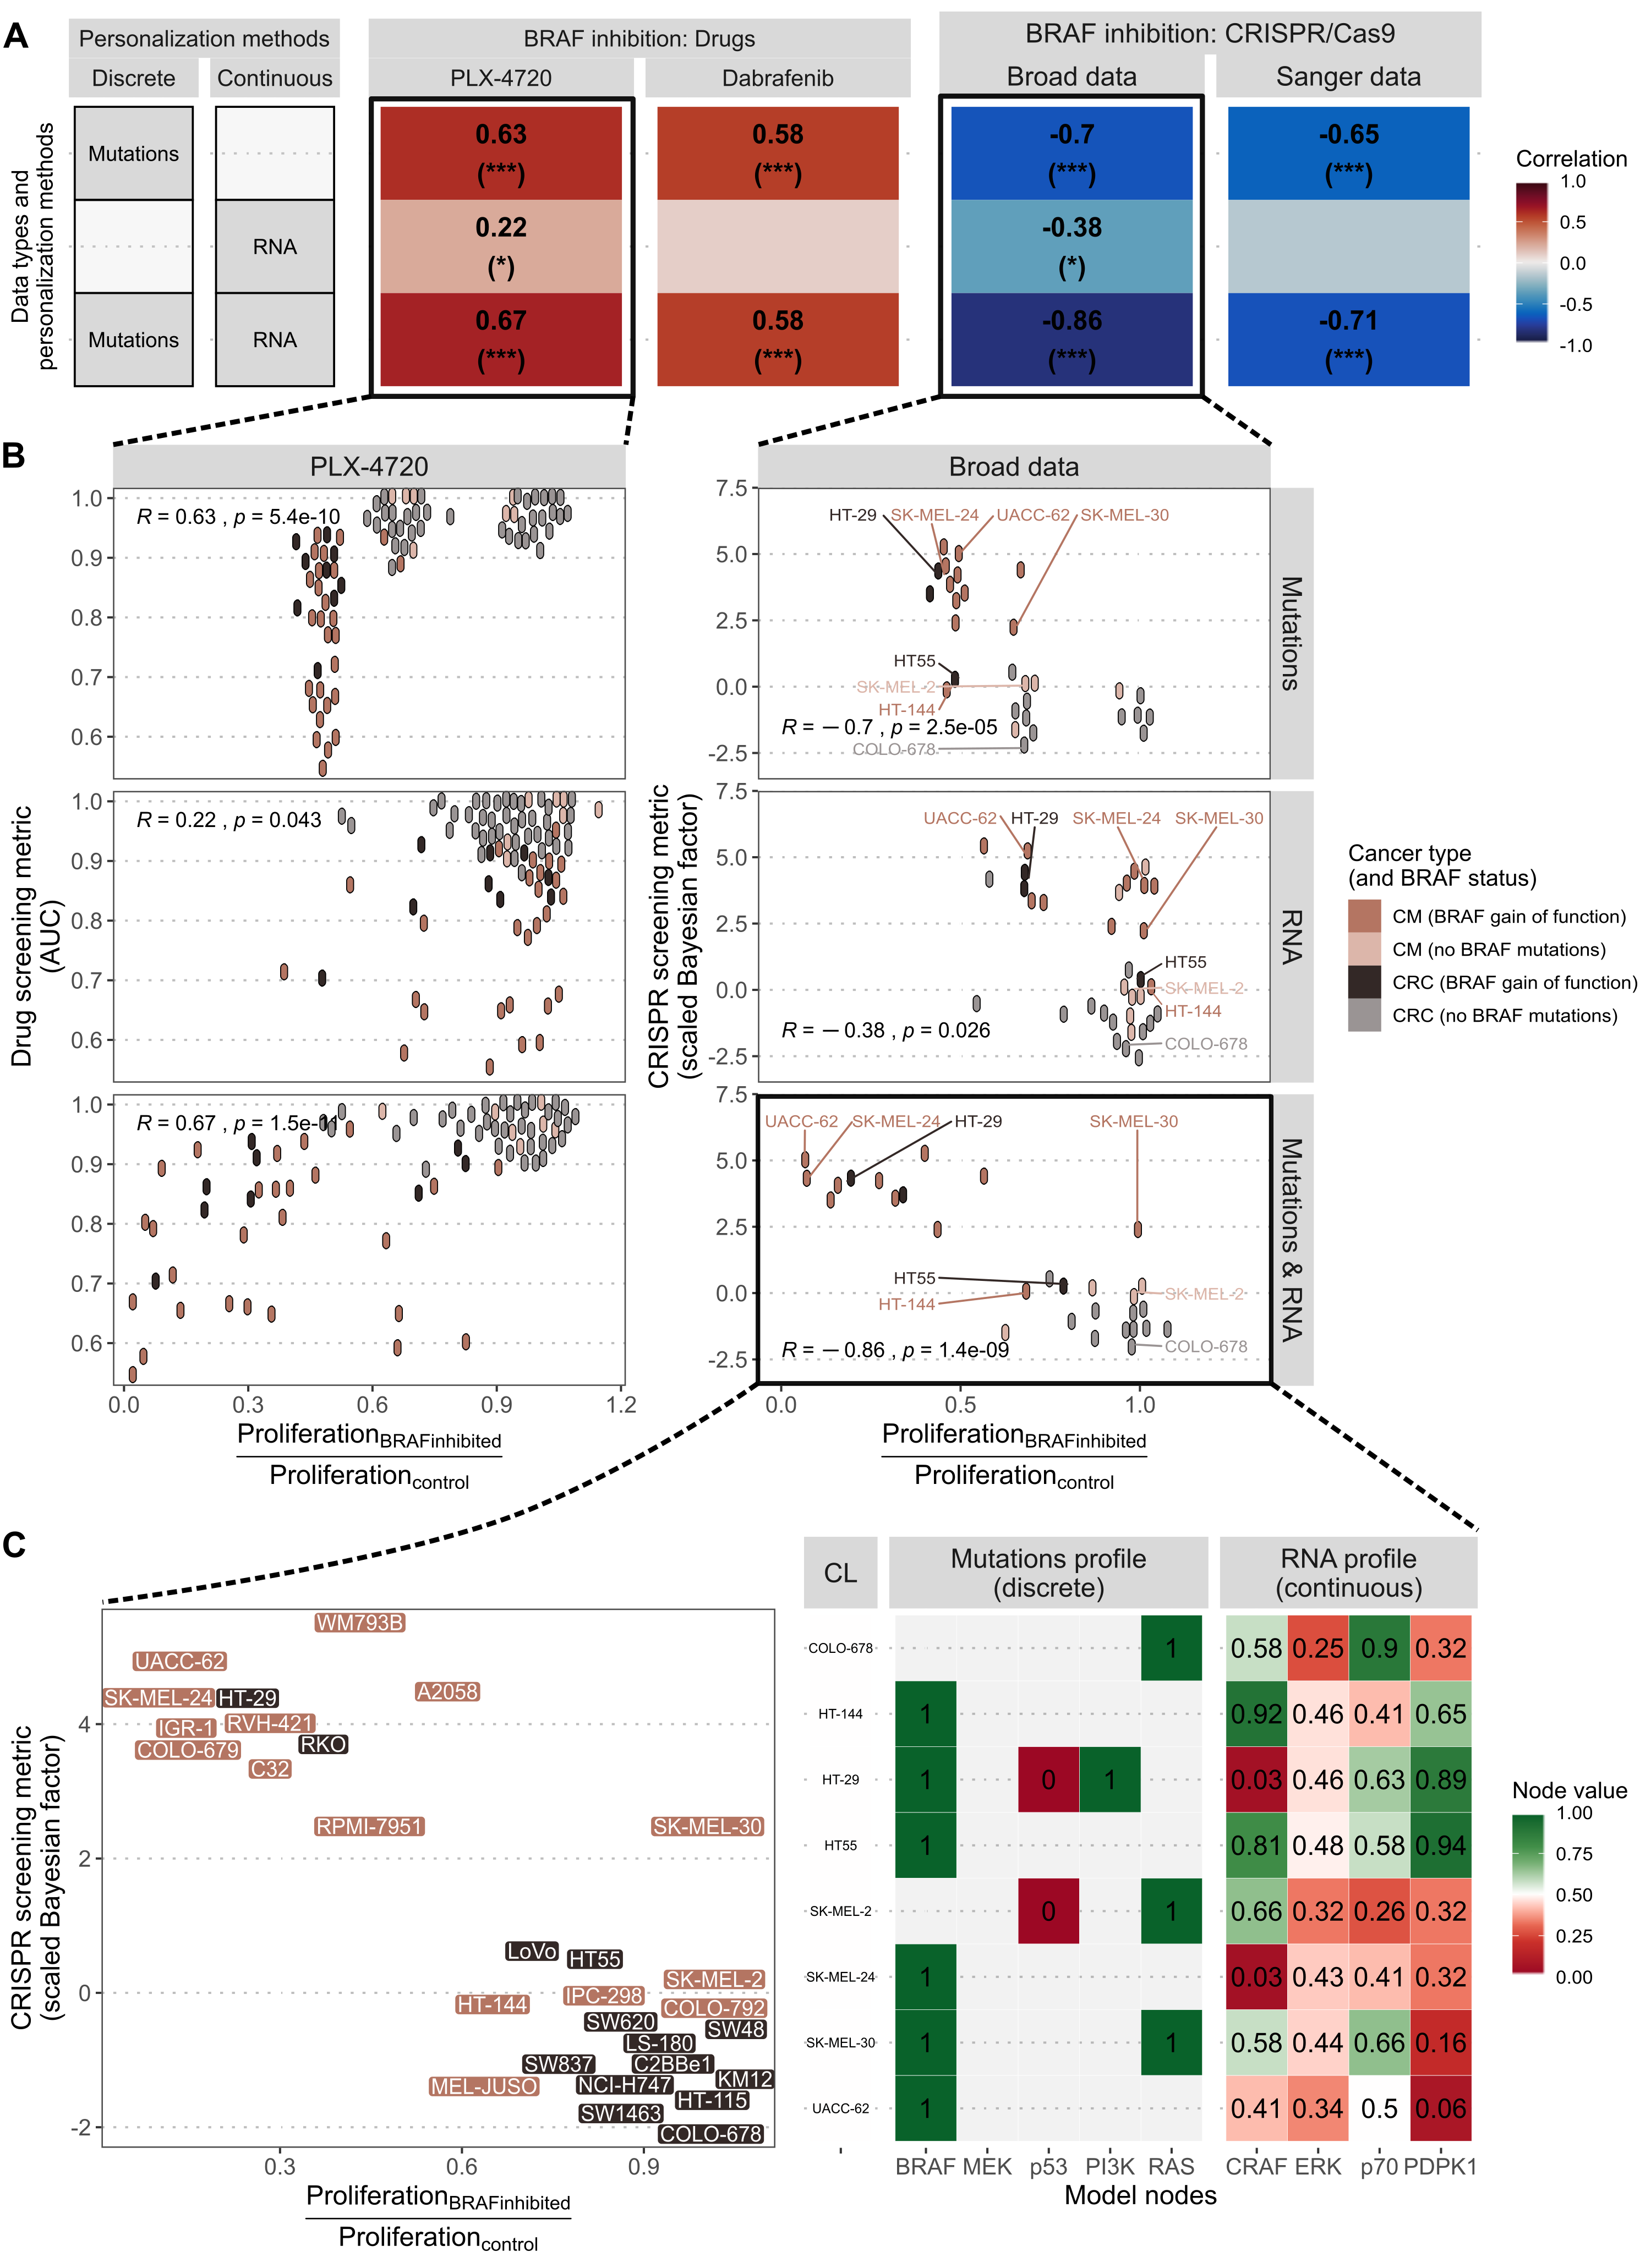
\includegraphics[width=0.9\linewidth]{fig/BRAF-results} 

}

\caption[Validation of personalized models of BRAF inhibition with cell lines data]{\textbf{Validation of personalized models of
BRAF inhibition with cell lines data.} (A) Pearson correlations between
normalized \emph{Proliferation} scores from personalized models and
experimental sensitivities to BRAF inhibition by drug or CRISPR
targeting; each row corresponds to a different personalization strategy;
only the values for the significant correlations are displayed. (B)
Scatter plots with non-overlapping points corresponding to correlations
of panel A, with the three personalization strategies, focusing on one
drug (PLX-4720) and one CRISPR dataset (Broad). (C) Enlargement of one
scatter plot in B (left) with the table describing the omics profiles
used for each cell line to explore the response mechanisms; interactive
version in Figure \ref{fig:BRAF-interactive} or
\href{https://github.com/sysbio-curie/PROFILE_BRAF_Model/blob/master/Analysis.html}{GitHub
files}.}\label{fig:BRAF-results}
\end{figure}
















The first approach consists in using only mutations as discrete
personalization (Figure \ref{fig:BRAF-results}, A, upper row): the
mutations identified in the dataset and that are present in the
regulatory network are set to 1 for activating mutations and set to 0
for inactivating mutations. In this case, the \emph{Proliferation}
scores from personalized models significantly correlate with both BRAF
drug inhibitors (PLX-4720 and Dabrafenib) and both CRISPR datasets
(using Pearson correlations). Note that the opposite directions of the
correlations for the drug and CRISPR datasets are due to the fact that
cell lines sensitive to BRAF inhibition result in low AUCs, and high
scaled Bayesian factors, respectively, and, if the models are relevant,
to low standardized \emph{Proliferation} scores. Looking more closely at
the corresponding scatter plot for PLX-4720 (Figure
\ref{fig:BRAF-results}B, upper left), it can be seen that this
correlation results from the \textbf{model's ability to use mutations'
information to recover the highest sensitivity of the BRAF-mutated cell
lines} that form an undifferentiated cluster on the left side. These
cell lines are indeed relatively more sensitive than non-mutated BRAF
cell lines. However, the integration of mutations alone does not explain
the significant differences within this subgroup (AUC between 0.55 and
0.9). A very similar behaviour can be observed when comparing model
simulations with CRISPR data (Figure \ref{fig:BRAF-results}B, upper
right).

Using only RNA data as continuous personalization (Figure
\ref{fig:BRAF-results}A and B, middle rows) is both less informative and
more difficult to interpret. For continuous data such as RNAseq data, we
normalize the expression values and set both the initial conditions and
the transition rates of the model variables to the corresponding values.
Correlations with experimental BRAF inhibitions appear weaker and more
uncertain. The key point, however, is that the \textbf{combination of
mutations and RNA, as depicted in Figure \ref{fig:BRAF-results} A and B
lower rows, seems to be more relevant}. This is partially true in
quantitative terms but it is even easier to interpret in the
corresponding scatter plots (Figure \ref{fig:BRAF-interactive}).
Comparing first the Broad CRISPR scatter plots using mutations only
(Figure \ref{fig:BRAF-results}B, upper right) and using both mutations
and RNA (Figure \ref{fig:BRAF-results}B, lower right), we can observe
that non-responsive cell lines (scaled Bayesian factor below 0), grouped
in the lower right corner and correctly predicted using only mutations
stayed in the same area: these strong mutational phenotypes have not
been displaced by the addition of RNA data. Other cell lines previously
considered to be of intermediate sensitivity by the model (e.g.,
COLO-678 or SK-MEL-2) were shifted to the right, consistent with the
lack of sensitivity observed experimentally. Finally, BRAF-mutated cell
lines, previously clustered in one single column on the left using only
mutations (with normalized \emph{Proliferation} scores around 0.5), have
been moved in different directions. Many of the most sensitive cell
lines (scaled Bayesian factor above 2) have been pushed to the left in
accordance with the high sensitivities observed experimentally (e.g.,
HT-29 or SK-MEL-24). It is even observed that the model corrected the
position of the two BRAF mutated cell lines, but whose sensitivity is
experimentally low (melanoma cell line HT-144 and colorectal cell line
HT-55). Only one cell line (SK-MEL-30) has seen its positioning evolve
counter-intuitively as a result of the addition of RNA in the
personalization strategy: relatively sensitive to the inhibition of
BRAF, it has, however, seen its standardised \emph{Proliferation} score
approach 1. All in all, this contribution of RNA data results in
significant correlations even when restricted to BRAF-mutated cell lines
only (\(R=0.69\), \(p.value=0.006\)).

\begin{figure}

{\centering \includegraphics[width=0.9\linewidth]{06-Drugs_files/figure-latex/BRAF-interactive-1} 

}

\caption[Interactive]{\textbf{Multi-omics integration and
enhanced value of RNA in addition to mutations.} For each cell line, an
arrow shows the impact of adding RNA in the customization strategy. This
graph is present in an interactive format in the online version of the
thesis in order to give easy access to the omic profile corresponding to
each point.}\label{fig:BRAF-interactive}
\end{figure}








A similar analysis can be made of the impact of adding RNA data to
personalization when comparing with the experimental response to
PLX-4720 (Figure \ref{fig:BRAF-results}B, upper and lower left). Most of
the non-sensitive cell lines (upper right corner) have not seen the
behaviour of the personalized models change with RNA addition. However,
the numerous BRAF-mutated cell lines previously grouped around
standardized \emph{Proliferation} scores of 0.5, are now better
differentiated and their sensitivity predicted by personalized models
has generally been revised towards lower scores (i.e., higher
sensitivity). Similar to the CRISPR data analysis, three sensitive cell
lines have been shifted to the right and are misinterpreted by the
model. As a result, the correlation restricted to BRAF-mutated cell
lines is no longer significant (R=0.26, p.value=0.1).

\subsubsection{An investigative tool}\label{an-investigative-tool}

These \textbf{personalized models are not primarily intended to be
predictive tools but rather used to reason and explore the possible
mechanisms and specificities of each cell line, for example by studying
the molecular alterations at the origin of the observed behaviour}
(Figure \ref{fig:BRAF-interactive}). To continue on the previous
examples, the two melanoma cell lines, HT-144 and SK-MEL-24, share the
same mutational profiles but have very different sensitivities to BRAF
targeting (Figure \ref{fig:BRAF-results}C). This inconsistency is
partially corrected by the addition of the RNA data, which allows the
model to take into account the difference in CRAF expression between the
two cell lines. In fact, CRAF is a crucial node for the network since it
is necessary for the reactivation of the MAPK pathway after BRAF
inhibition. Therefore, the high sensitivity of SK-MEL-24 may be
explained by its low CRAF expression level, which makes the reactivation
of the MAPK pathway more difficult for this cell line. Conversely, in
HT-144, the high level of CRAF expression allows the signal to flow
properly through this pathway even after BRAF inhibition, thus making
this cell line more resistant. The importance of CRAF expression is also
evident in HT-29, a CRC BRAF mutated cell line with other important
mutations (PI3K activation and p53 deletion). However, it remains
sensitive to treatment, due to its very low level of CRAF expression.

Another interesting contribution of RNA appears in the melanoma cell
line UACC-62, which is particularly sensitive to treatment. The model is
able to correctly predict its response once RNA levels are integrated.
In this case, the reason for sensitivity seems to be due to the low
level of PDPK1, which makes it difficult to activate p70 and thus
trigger the resistance linked to PI3K/AKT pathway activation. Similarly,
the CRC resistant cell line, HT55, which carries only the BRAF mutation,
expresses high levels of PDPK1, in addition to high levels of CRAF,
supporting the idea that the presence of both MAPK and PI3K/AKT pathways
may confer resistance to BRAF inhibition treatments. We can also mention
a cluster of RAS mutated cell lines, usually NRAS mutated for melanomas
(e.g., SK-MEL-2) and KRAS for colorectal cancers (e.g., COLO-678), which
are classified by the model as resistant. Interestingly, in these cell
lines, a low level of CRAF is not enough to block the signal of the MAPK
pathway, which is stronger in the model because of the simulation of the
RAS mutation (RAS is set to \(1\)). Only SK-MEL-30 appears to be
incorrectly classified and is observed to be more sensitive than the
other cell lines with a similar mutation profile. This could be due to
the fact that our network is incomplete and not able to account for some
alterations responsible for this cell line sensitivity. The exploration
of the mutational profile for this cell line might be a hint of The
problem may also come from the fact that this cell line contains a
frameshift mutation of RPS6KB2 (p70 node) not referenced in OncoKB and
therefore not included in the simulation.

\begin{figure}

{\centering 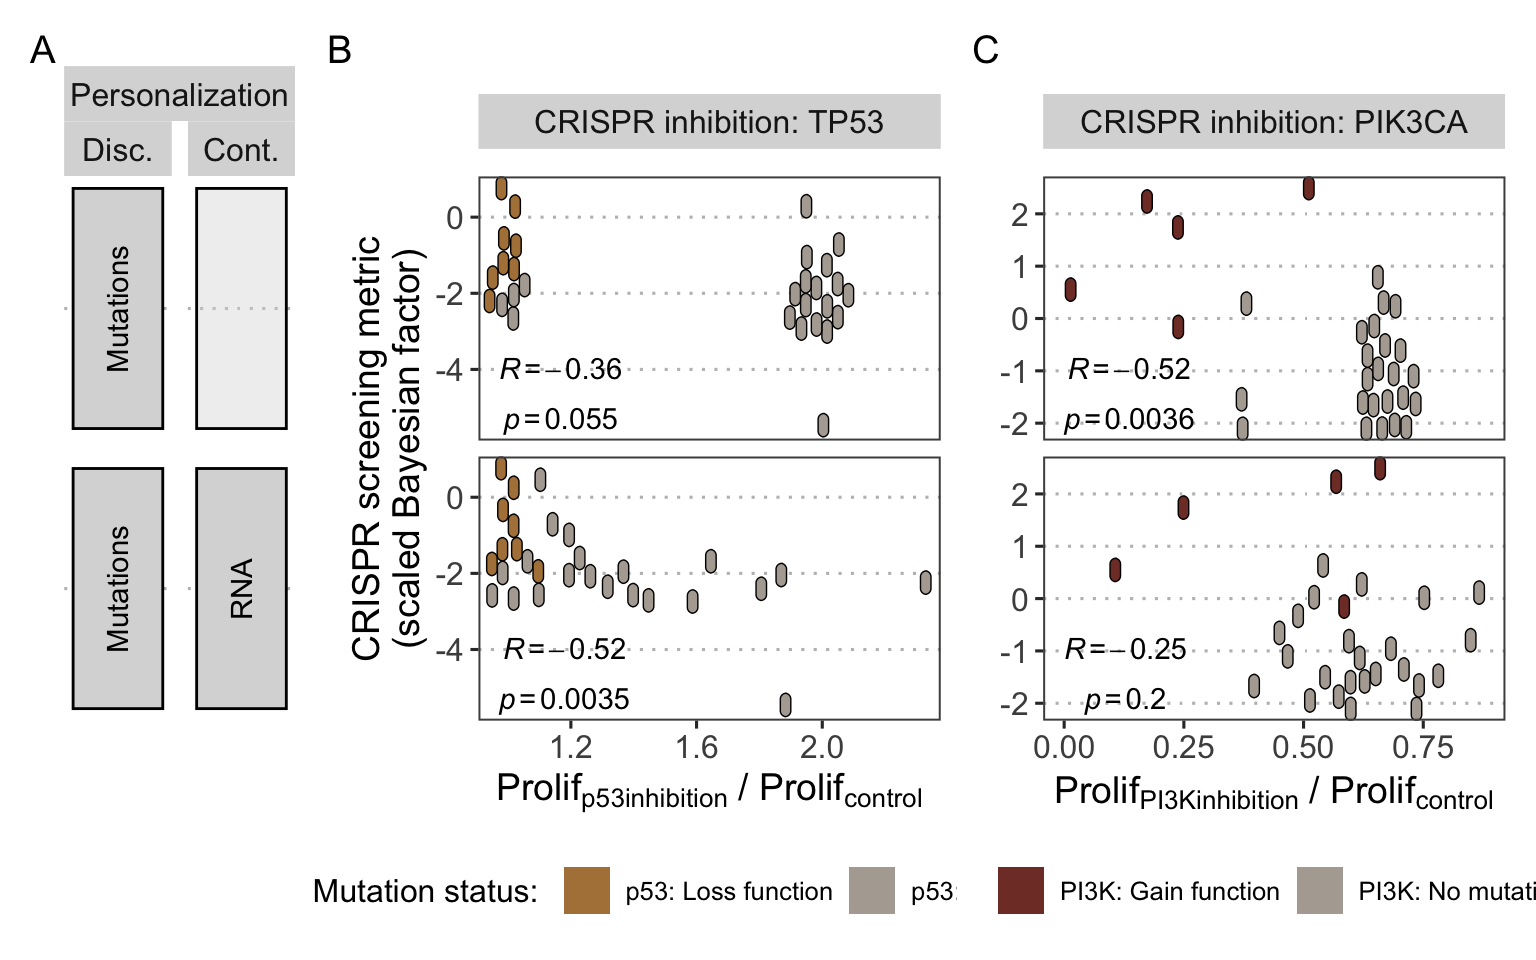
\includegraphics[width=0.9\linewidth]{06-Drugs_files/figure-latex/BRAF-results-add-1} 

}

\caption[Application of personalized models to other CRISPR targets]{\textbf{Application of personalized
models to other CRISPR targets.} (A) Personalization strategies using
either mutations only (as discrete data) or combined with RNA (as
continuous data) with their corresponding scatter plots in panels B and
C. (B) Scatter plot comparing normalized \emph{Proliferation} scores of
p53 inhibition in the models with experiment sensitivity of cell lines
to TP53 CRISPR inhibition, indicating p53 mutational status as
interpreted in the model. Pearson correlations and the corresponding
p-values are shown. (C) Similar analysis as in panel B with PI3K model
node and PIK3CA CRISPR inhibition.}\label{fig:BRAF-results-add}
\end{figure}












The versatility of the logical formalism makes it possible to test other
node inhibitions as in Figure \ref{fig:BRAF-results-add}, but remains
limited by the scope of the model. Since the present model has been
designed around BRAF, its regulators have been carefully selected and
implemented, which is not necessarily the case for other nodes of the
model. Therefore, these personalized models can be used to study how
comprehensive the descriptions of the regulation of other nodes or parts
of the model are. Thus, model simulations show that response trends to
TP53 inhibition are consistently recovered by the model (Figure
\ref{fig:BRAF-results-add}B) but the simple regulation of p53 in the
model results in coarse-grained patterns, although slightly improved by
addition of RNA data. Similar analyses regarding the targeting of PIK3CA
(in CRISPR data) simulated, in the model, by the inhibition of PI3K
node, can be performed (Figure \ref{fig:BRAF-results-add}C). \textbf{Low
correlations are an indication highlighting the insufficient regulation
of the node, probably confirming the scope issues raised in the
pan-cancer-preliminary analysis}.

\subsection{Comparison of the mechanistic approach with machine learning
methods}\label{comparison-of-the-mechanistic-approach-with-machine-learning-methods}

\begin{figure}

{\centering 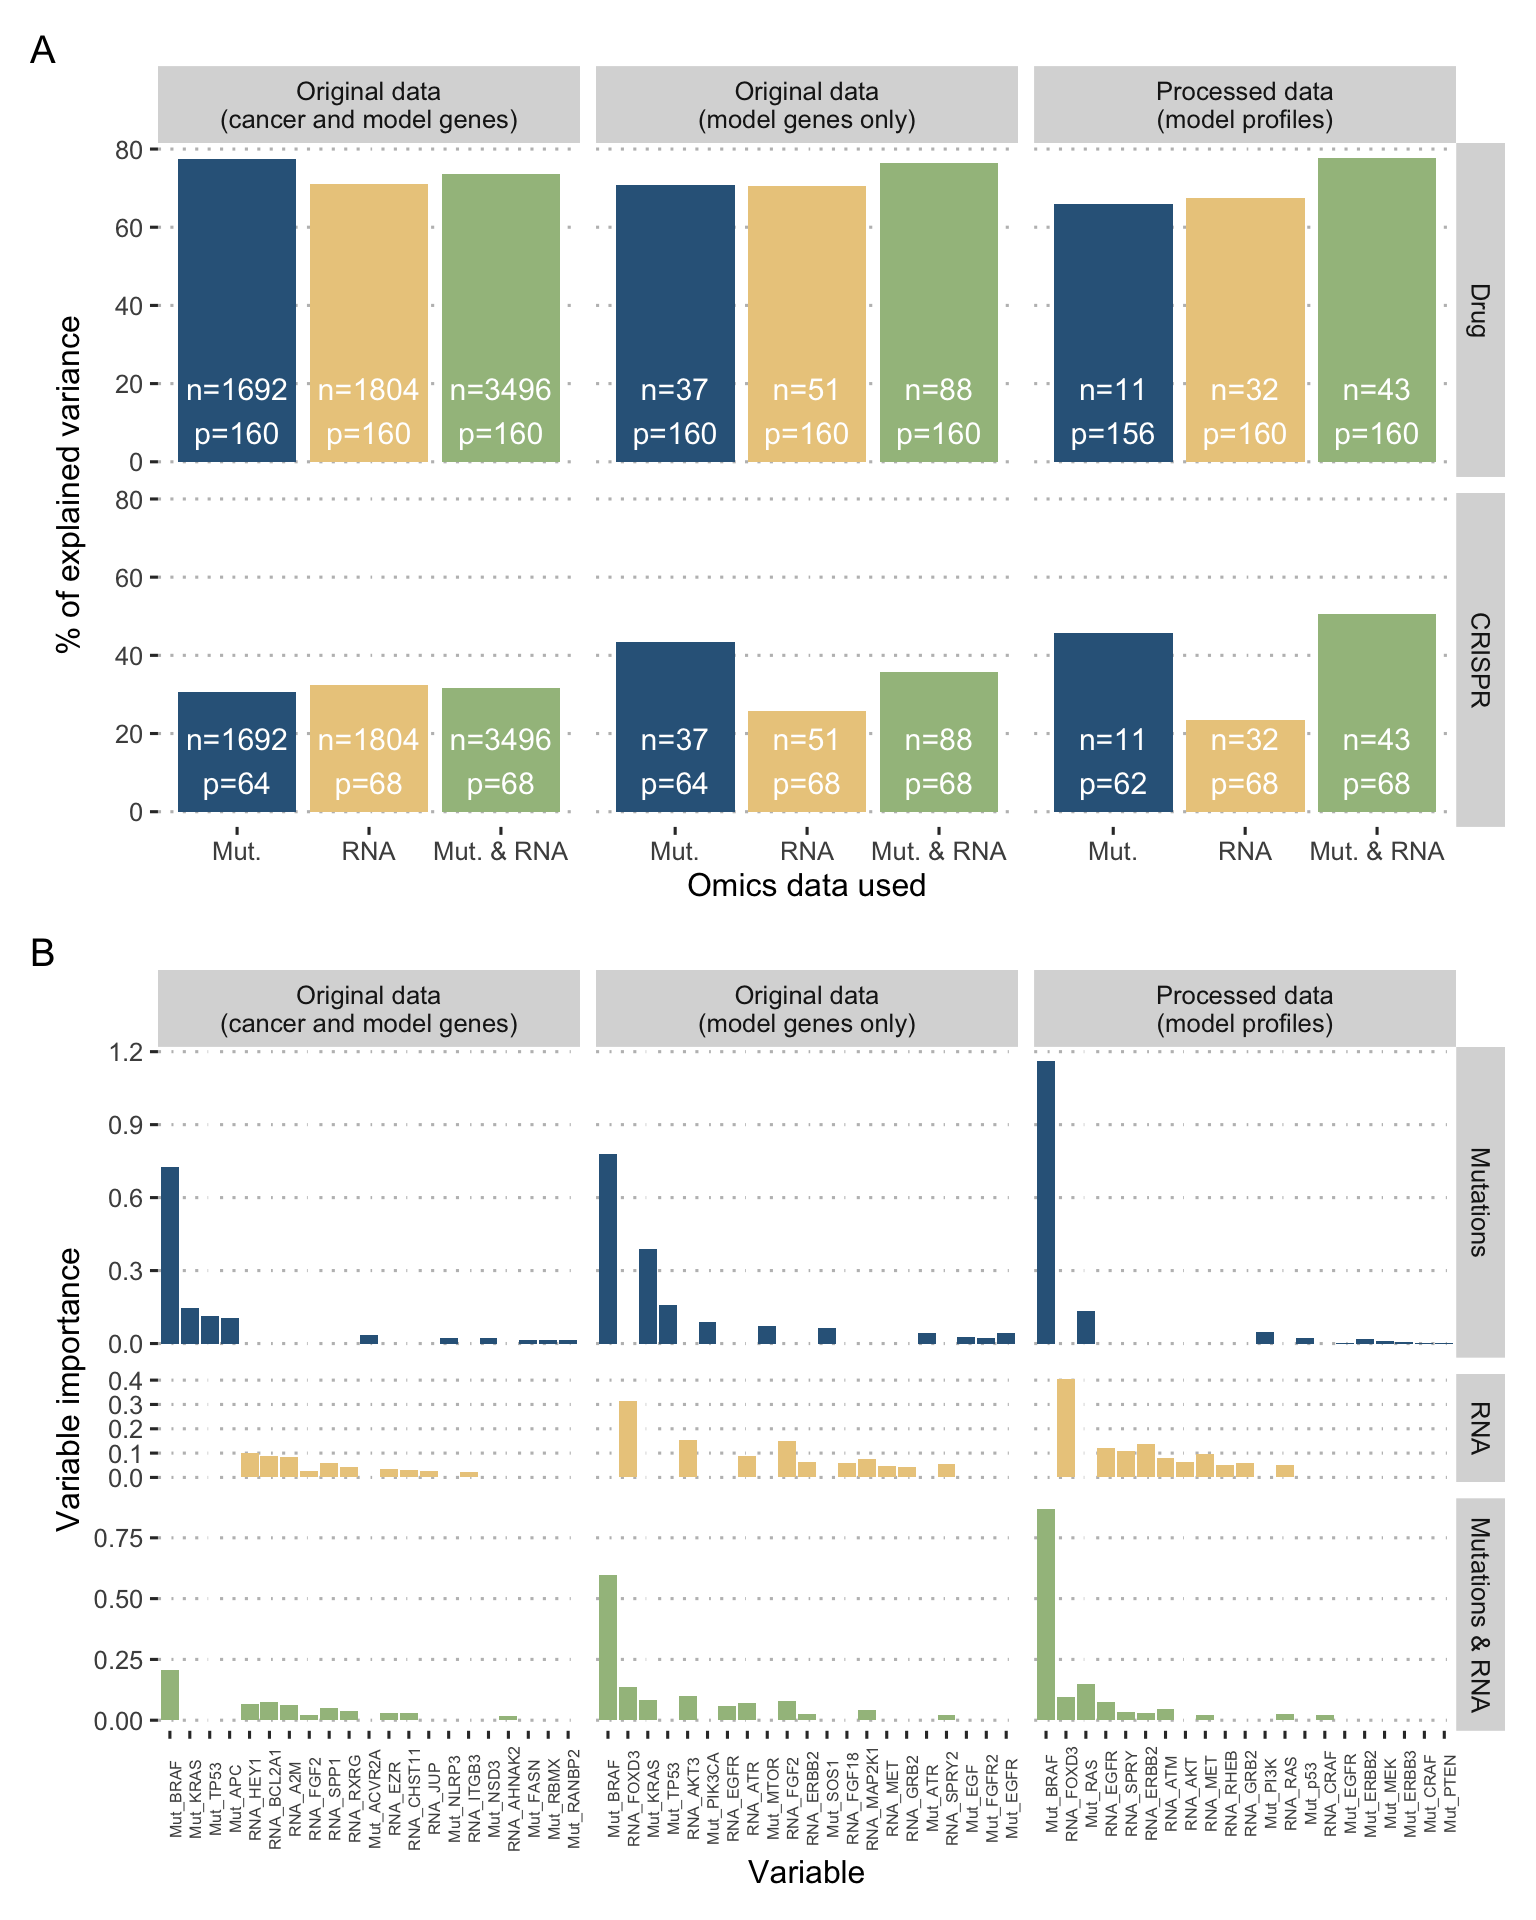
\includegraphics[width=0.9\linewidth]{06-Drugs_files/figure-latex/BRAF-ML-1} 

}

\caption[Application of personalized models to other CRISPR targets]{\textbf{Random forests to predict and explain
sensitivity to BRAF inhibition.} (A) Performances of random forests for
BRAF sensitivity prediction measured with percentage of explained
variance; different learning task with unprocessed original data
(thousands of genes), unprocessed original data for model-related genes
only (tens of genes), and processed profiles of cell lines (tens of
genes); \(n\) samples and \(p\) variables per learning task. (B)
Variable importance for drug prediction only, with the 10 best variables
with positive importance for each case.}\label{fig:BRAF-ML}
\end{figure}











In order to provide comparison elements unbiased by prior knowledge or
by the construction of the model, we performed some simple machine
learning algorithms. Random forests are used as an example of a machine
learning approach to compare with mechanistic models and are implemented
with \emph{randomForestSRC} R package \citep{breiman2001random}. Random
forests can be seen as an aggregation of decision trees, each trained on
a different training set formed by uniform sampling with replacement of
the original cohort. Prediction performances are computed using
out-of-the bag estimates for each individual (i.e, average estimate from
trees that did not contain the individual in their bootstrap training
sample) and summarized as percentage of variance explained by the random
forest. In this case, random forests have been fitted with inputs
(mutations and/or RNA data) and outputs (sensitivities to drug or CRISPR
BRAF inhibition) similar to those of logical models and the
corresponding predictive accuracies are reported in Figure
\ref{fig:BRAF-ML}A. The first insight concerns data processing. The
percentages of variance explained by the models are similar (around 70\%
of explained variance for drug sensitivity prediction) in the following
three cases: unprocessed original data (thousands of genes), unprocessed
original data for model-related genes only (tens of genes), and
processed profiles of cell lines (tens of genes). This supports the
choice of a model with a small number of relevant genes, which appear to
contain most of the information needed for prediction. Second, the
absolute level of performance appears much lower for CRISPR (between 30
and 50\%) probably suffering from the lower number of samples,
especially in cases where the number of variables is the highest. This
tends to \textbf{reinforce the interest of mechanistic approaches that
do not use any training on the data for smaller datasets, less suitable
for learning}. Finally, while mutations and RNA data seem to provide the
same predictive power (especially for drugs), using the two together
does not necessarily result in a better performance in this case.

It is also possible to compute the variable importance that assesses the
contribution of variables to the overall performance. The solution
adopted in this paper to measure it, and called VIMP in the package,
consists in introducing random permutations between individuals for the
values of a variable and quantifying the variation in performance
resulting from this addition of noise. In the case of key variables for
prediction, this perturbation will decrease the performance and will
result in a high variable importance \citep{ishwaran2007variable}.
\textbf{Variable importance in these different random forests are
reported in Figure \ref{fig:BRAF-ML}B and are consistent with the
analysis of mechanistic models}. The mutational status of BRAF is
definitely the most important variable followed by mutations in RAS or
TP53. Concerning RNA levels, the most explanatory variables seem to be
FOXD3 or PTEN, in line with the definition of the logical model.

\section{Application on prostate cancer study and
challenges}\label{prostate-model}

Before summarizing the potential and limitations of the PROFILE
approaches described in this and the previous chapter, a final example
may be mentioned. Indeed, another application of the PROFILE method,
quite similar to the examples presented in the previous and this
chapter, has been carried out on prostate cancer. Chronologically, this
project was one of the first applications of the method. However, as
this project was more collaborative than personal, the previous chapters
have been illustrated by more exclusively personal work when they were
equivalent. We will therefore only briefly mention here the differences
and insights specific to this study.

First, a logical model specific to prostate cancer was developed by some
collaborators (Pauline Traynard and Arnau Montagud) over a long period
of time, resulting in a large and comprehensive model of 146 nodes,
which is described in more detail in the appendix
\ref{appendix-montagud} and Figure \ref{fig:Montagud}. Using the TCGA
prostate cancer dataset (\ref{appendix-prostate}) prognostic validation
of the model was first carried out, similarly to Figure
\ref{fig:PROFILE-METABRIC-Grade}, by comparing individualized scores of
some phenotypes in the model (i.e. \emph{Proliferation}) with clinical
markers, in this case Gleason score, a grading system specific to
prostate cancer. The qualitative evolution of the personalized
\emph{Proliferation} scores is also qualitatively validated (predicted
proliferating tumors are on average of higher grade) but, despite the
specificity and magnitude of the model, much of the variability is not
explained.

The use of cell line data was also explored using Cell Model Passports
data, restricted to the 7 prostate cell lines. The size of the model
then allows qualitative predictions to be made on the proliferative,
apoptotic and metastatic qualities of the different lines. Except for
proliferation, however, experimental validation of the relevance of
these predictions is difficult using public data or the literature. But
again, after these preliminary validations, the focus of the study was
on treatment response with a slightly different rationale than in the
previous example. Focusing on a particular cell line (LnCaP) and its
corresponding personalized logical model, the idea is to
\textbf{simulate with the models all possible inhibitions or
combinations of inhibitions in order to identify possible
vulnerabilities or relevant treatment synergies}. Experimental
validation on the cell line was then carried out for certain genes that
could be targeted depending on the existence of the treatments. The
\textbf{efficacy of certain inhibitions highlighted by the simulations,
such as that of HSP90, was confirmed experimentally} on this particular
cell line. Despite the limitations of the approach in this application
to prostate cancer, the study demonstrates the feasibility of the method
for investigating the complexity of therapeutic responses and guiding
experimental validation.

\section{Limitations and
perspectives}\label{limitations-and-perspectives}

The emergence of high-throughput data has made it easier to generate
models for prognostic or diagnostic predictions in the field of cancer.
The numerous lists of genes, biomarkers and predictors proposed have,
however, often been difficult to interpret because of their sometimes
uncertain clinical impact and little overlap between competing
approaches \citep{domany2014using}. Methods that can be interpreted by
design, which integrate \emph{a priori} biological knowledge, therefore
appear to be an interesting complement able to reconcile the omics data
generated and the knowledge accumulated in the literature.

These benefits come at the cost of having \textbf{accurate expert
description of the problem} to provide a relevant basis to the
mechanistic models. This is particularly true in this work since the
personalized models all derive from the same structure (the initial
generic logical model) of which they are partially constrained versions.
It is therefore necessary to have a generic model that is both
sufficiently accurate and broad enough so that the data integration
allows the expression of the singularities of each cell line. If this is
not the case, the learning of logical rules or the use of ensemble
modeling could be favoured, usually including perturbation time-series
data \citep{razzaq2018computational}. It should also be noted that, in
the logical models presented here, the translation of biological
knowledge into a logical rule is not necessarily deterministic and
unambiguous. The choices here have been made based on the interpretation
of the literature only. And the presence of certain outliers, i.e., cell
lines whose behaviour is not explained by the models, may indeed result
from the limitations of the model, either in its scope (important genes
not integrated), or in its definition (incorrect logical rules). More
global or data-driven approaches to define the model would be possible
but would require different training/validation steps and different sets
of data.

The \textbf{second key point is the omics data used}. For practical
reasons, we have focused on mutation and RNA data. The legitimacy of the
former is not in doubt, but their interpretation is, on the other hand,
a crucial point whose relevance must be systematically verified. The
omission or over-interpretation of certain mutations can severely affect
the behaviour of personalized models. Validation using sensitivity data
provides a good indicator in this respect. However, the question is
broader for RNA data: are they relevant data to be used to personalize
models, i.e., can they be considered as \textbf{good proxies for node
activity?} The protein nature of many nodes in the model would encourage
the use of protein level data instead, or even phosphorylation levels if
they were available for these data. One perspective could even be to
push personalization to the point of defining different types of data or
even different personalization strategies for each node according to the
knowledge of the mechanisms at work in the corresponding biological
entity. A balance should then be found to allow a certain degree of
automation in the code and to avoid overfitting.

Despite these limitations, the results described above support the
\textbf{importance of combining the integration of different types of
data to better explain differences in drug sensitivities}. There was no
doubt about this position of principle in general
\citep{azuaje2017computational}, and in particular in machine learning
methods \citep{costello2014community, aben2016tandem}. The technical
implementation of these multi-omic integrations is nevertheless more
difficult in mechanistic models where the relationships between the
different types of data need to be more explicitly formulated
\citep{klinger2013network}. The present work therefore reinforces the
possibility and value of integrating different types of data in a
mechanistic framework to improve relevance and interpretation and
illustrates this by highlighting the value of RNA data in addition to
mutation data in predicting the response of cell lines to BRAF
inhibition. In addition, one piece of data that could be further
exploited is that of the specific behaviour of the drugs or inhibitors
studied, since for instance some BRAF inhibitors have affinities that
vary according to mutations in the BRAF gene itself. The integration of
truly precise data on the nature of the drug is nevertheless limited by
logical formalism and is more often found in more flexible approaches,
e.g.~in deep learning \citep{manica2019toward}.

To conclude, we provide a comprehensive pipeline from clinical question
to a validated mechanistic model which uses different types of omics
data and adapts to dozens of different cell lines. This work, which is
\textbf{based only on the interpretation of data and not on the training
of the model}, continues some previous work that has already
demonstrated the value of mechanistic approaches to answer questions
about response to treatment, especially using dynamic data
\citep{saez2020personalized}, and sometimes about similar pathways
\citep{klinger2013network}. In this context, our approach proves the
interest of logical formalism to make use of scarce and static data
facilitating application to a wide range of issues and datasets in a way
that is sometimes complementary to learning-based approaches.

\appendix \addcontentsline{toc}{chapter}{\appendixname}


\chapter{About datasets}\label{appendix-datasets}

\section{Cell lines}\label{appendix-cl}

Several analyses in previous chapters are based on data derived from
cell lines. Among the different databases, the ones used in the thesis
are briefly described below. Please refer to corresponding references
for additional details.

\subsection{Omics profiles}\label{omics-profiles}

The omics profiles of cancer cell lines have been downloaded from Cell
Model Passports \citep{van2019cell} containing genotypic and phenotypic
information about more than 1000 cell lines. Among the available data
used in this thesis are the exome sequencing, copy number variations and
RNA-sequencing.

\subsection{Drug screenings}\label{appendix-GDSC}

Information about response to treatments is retrieved from Genomics of
Drug Sensitivity in Cancer Database (GDSC, \citet{yang2012genomics}). In
order to allow detailed analyses at the level of cancer types, we will
restrict ourselves here to tissues represented by at least 20 cell lines
and highlighted in dark grey in Figure \ref{fig:GDSC}A. Most of the 663
cell lines in this subcohort have a complete profile with all omics data
(mutations, CNA and expression) and drug responses. However, not all
cell lines have necessarily been tested for all drugs.

\begin{figure}

{\centering 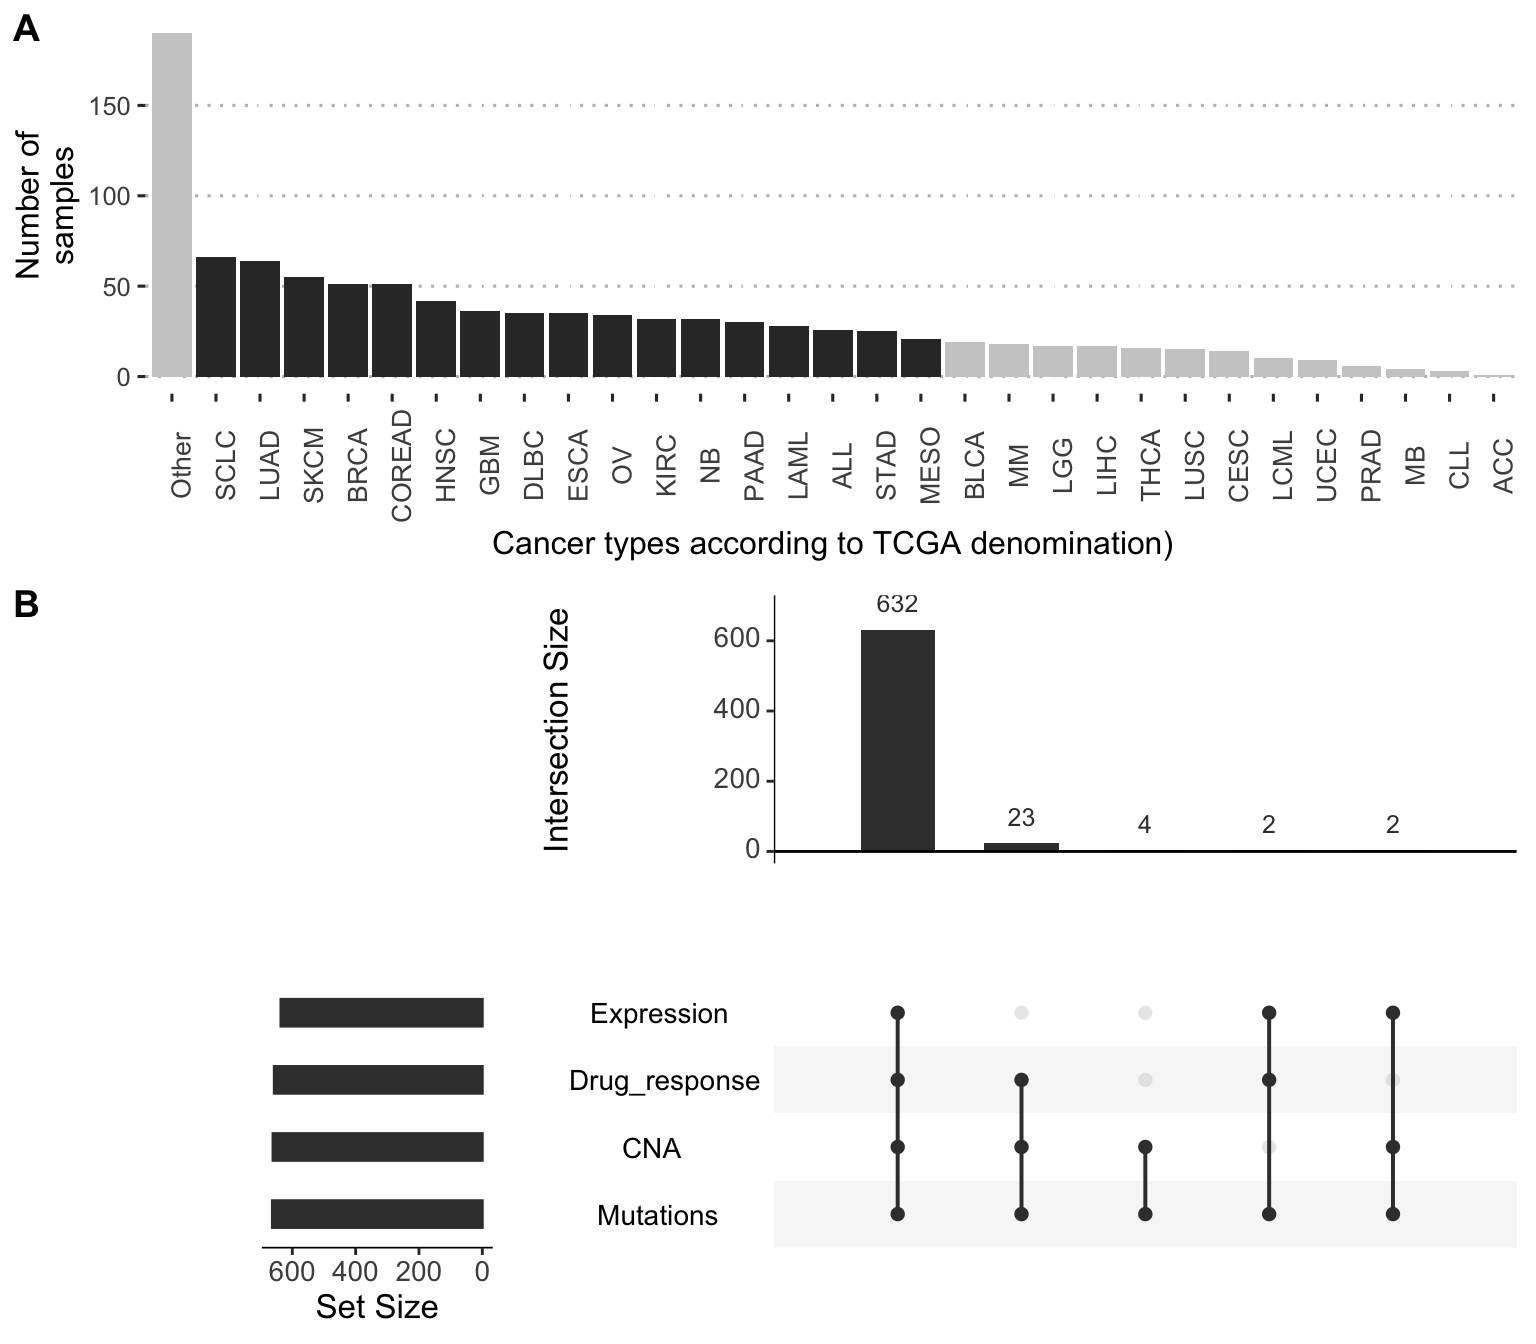
\includegraphics[width=0.9\linewidth]{10-Appendix_files/figure-latex/GDSC-1} 

}

\caption[Distribution of cancer types and data types in GDSC-associated dataset]{\textbf{Distribution of cancer types and data types
in GDSC-associated dataset.} (A) Distribution of cell lines per cancer
types, highlighting the ones selected in this thesis with more than 20
cell lines. (B) Availibility of data for the 663 selected cell lines in
17 different cancer types.}\label{fig:GDSC}
\end{figure}







The cell lines are treated with increasing concentration of drugs and
the viability of the cell line relative to untreated control is
measured. The dose-response relative viability curve is fitted and then
used to compute the half maximal inhibitory concentration (\(IC_{50}\))
and the area under the dose-response curve (AUC)
\citep{vis2016multilevel}, both being represented in Figure. Since the
\(IC_{50}\) values are often extrapolated outside the concentration
range actually tested, we will focus on the AUC metric for all
validation with drug screening data. AUC is a value between 0 and 1:
values close to 1 mean that the relative viability has not been
decreased, and lower values correspond to increased sensitivity to
inhibitions. In cases where the ranges of concentrations tested for
different drugs vary, comparison of their AUC values does not have a
simple and straightforward interpretation.

\begin{figure}

{\centering 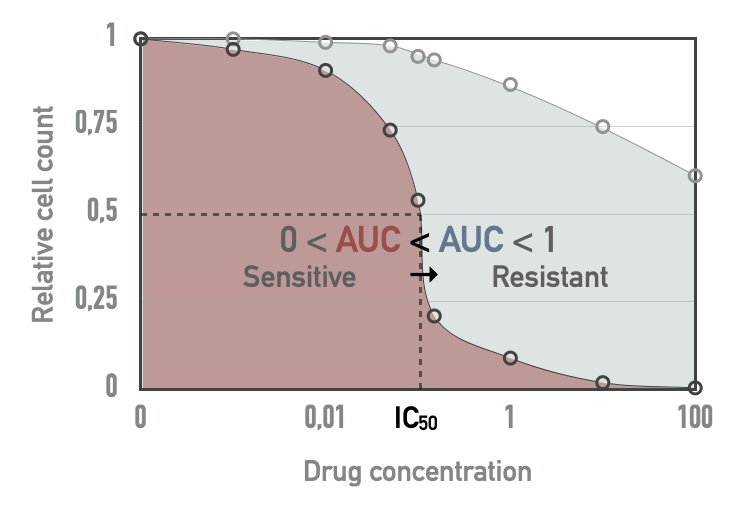
\includegraphics[width=0.5\linewidth]{fig/AUC} 

}

\caption[Drug screening metrics in cell lines]{\textbf{Drug screening metrics in cell lines.} Based
on a tested drug concentration range, \(IC_{50}\) and area under the
dose-response curve (AUC) can be computed. For a given drug, red AUC
corresponds to a more sensitive cell line than blue AUC.}\label{fig:AUC}
\end{figure}






\subsection{CRISPR-Cas9 screening}\label{appendix-CRISPR}

On top the previous drug response characterization, some CRISPR-Cas9
screenings have been performed on cancer cell lines. Very basically,
this involves using single-guide RNAs (sgRNAs) to direct the targeted
inhibition of certain genes. Conceptually, screening is not very
different from drug screening since it allows the sensitivity of cell
lines to the inhibition of certain targets to be studied. However, this
technology makes it possible to target many more different genes since
it is based on RNA guide synthesis and not on the existence of drugs
with an affinity for the target of interest. Schematically, sreening is
therefore broader (thousands of genes), less biased (any gene can be
targeted a priori) and more precise (much lower off-target effect).

Among the various databases available, the ones used in this thesis have
been downloaded from Cell Model Passports and come from Sanger Institute
\citep{behan2019prioritization} and Broad Institute
\citep{meyers2017computational}. Both databases present CRISPR
inhibition results for thousands of genes for a few hundred cell lines
among those presented in the previous section. The Sanger dataset for
instance includes 324 cell lines, and 238 in common with the subcohort
previously described in the previous section and in Figure
\ref{fig:GDSC}.

Among the different metrics, the examples presented in this thesis will
focus on scaled Bayesian factors to assess the effect of CRISPR
targeting of genes. These scores are computed based on the fold change
distribution of sgRNA \citep{hart2016bagel}. The highest values indicate
that the targeted gene is essential to the cell fitness.

\section{Patient-derived xenografts}\label{patient-derived-xenografts}

Distributions and some figures

\section{Patients}\label{appendix-datasets-patients}

\subsection{METABRIC}\label{metabric}

METABRIC dataset is large breast cancer dataset with more than 2000
patients \citep{pereira2016somatic}. Mutations, CNA, expression
(transcriptomics micro-array) and clinical data are available for a
majority of patients (Figure \ref{fig:METABRIC}A), with 1904 patients
for whom all the data is available. One of the particular features of
these data is to propose a very long clinical follow-up, over more than
10 years (Figure \ref{fig:METABRIC}B).

\begin{figure}

{\centering 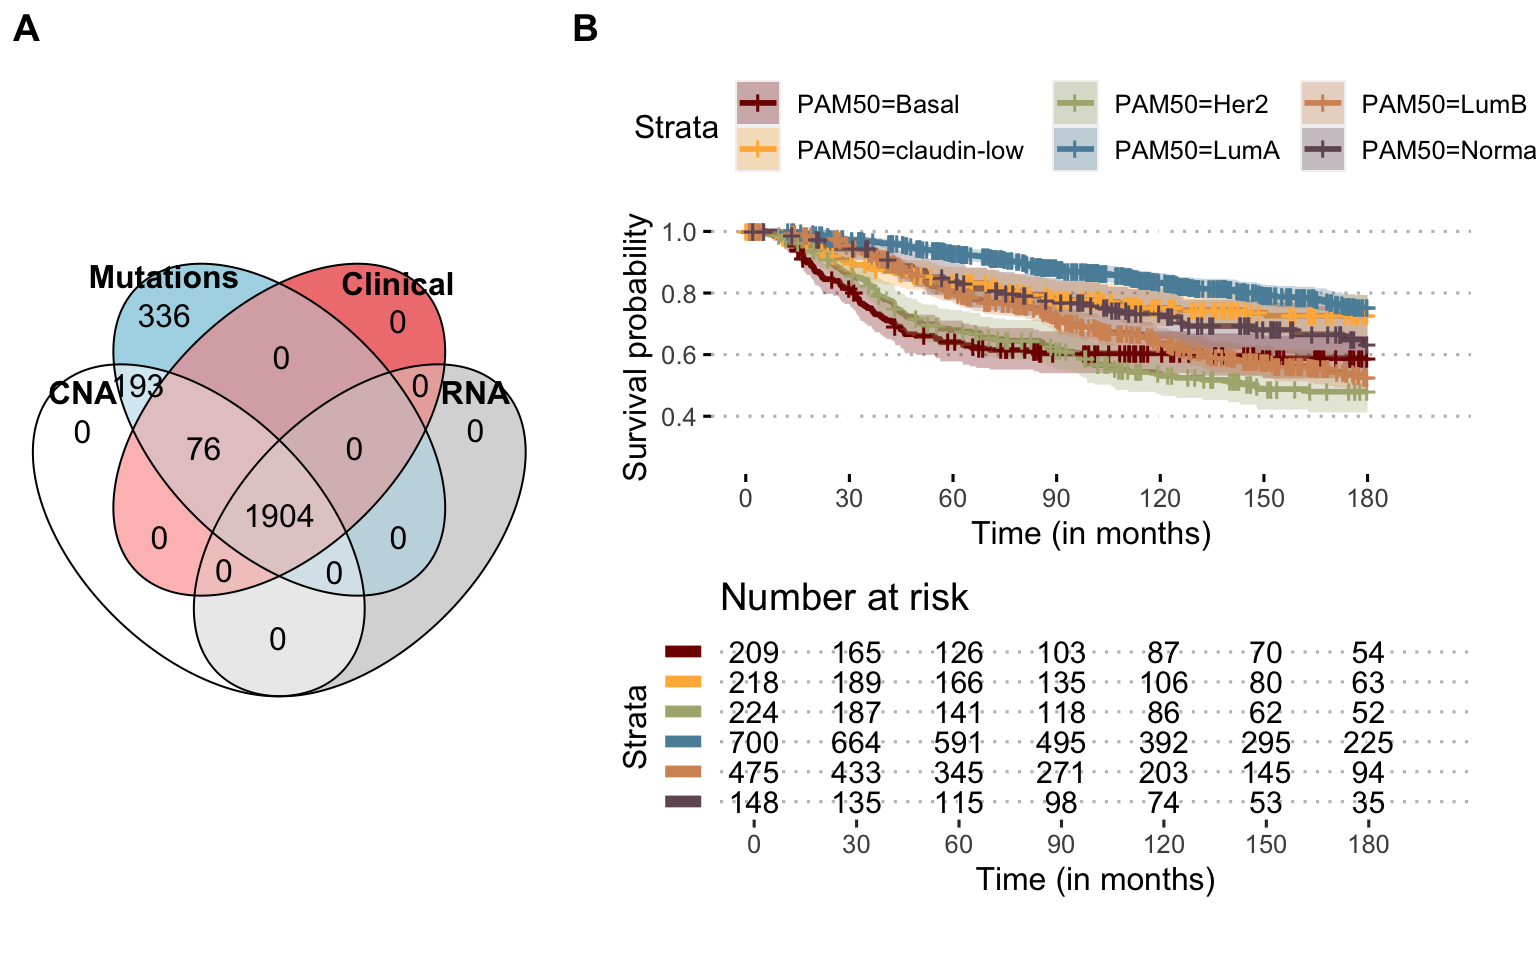
\includegraphics[width=0.9\linewidth]{10-Appendix_files/figure-latex/METABRIC-1} 

}

\caption[Available omics and survival in METABRIC Breast Cancer dataset]{\textbf{Available omics and survival in METABRIC
Breast Cancer dataset}. (A) Number of patients for each omics type and
their combinations, depicted as a Venn diagram. (B) Overall survival
probability for all patients with clinical follow-up, stratified per
breast cancer PAM50 subtype; administrative censoring at 180 months.}\label{fig:METABRIC}
\end{figure}







\subsection{TCGA: Breast cancer}\label{tcga-breast-cancer}

Another reference database for breast cancer is the one from the TCGA
consortium \citep{cancer2012comprehensive}. The cohort is smaller than
METABRIC and its clinical follow-up is more limited. In contrast, the
omics data are more comprehensive and include RNA sequencing and
relative quantification ofsproteins with RPPA technology (Figure
\ref{fig:TCGA-bp}A).

\begin{figure}

{\centering 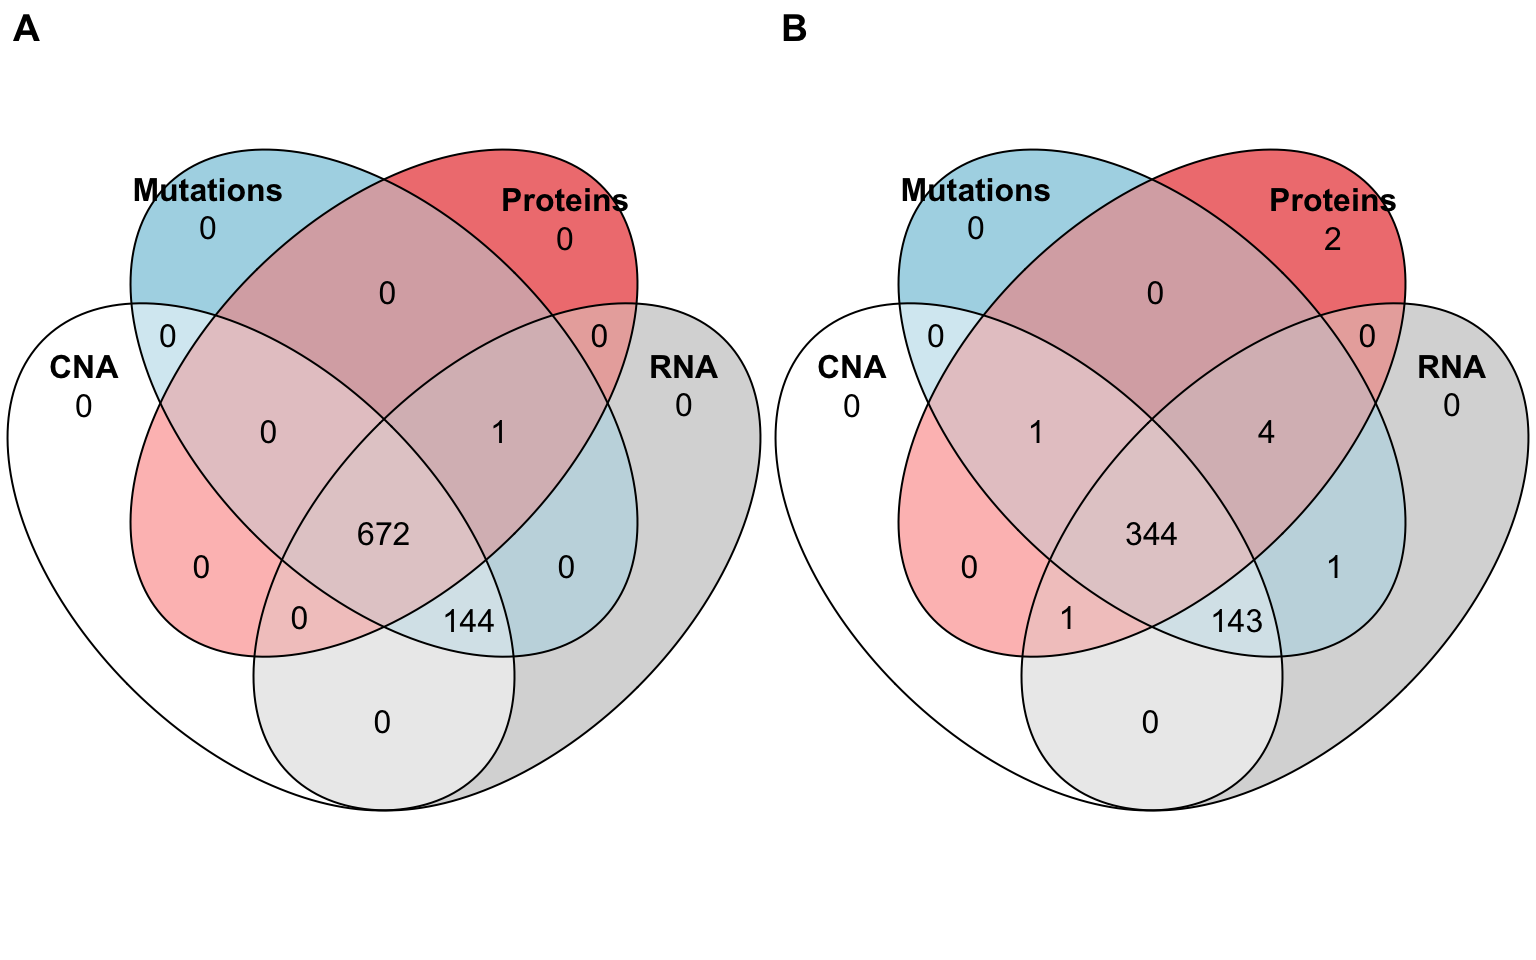
\includegraphics[width=0.7\linewidth]{10-Appendix_files/figure-latex/TCGA-bp-1} 

}

\caption[Available omics and survival in METABRIC Breast Cancer dataset]{\textbf{Available omics for TCGA Breast and
Prostate cancer}. (A) Number of patients for each omics type and their
combinations, depicted as a Venn diagram, in TCGA BRCA (Breast Invasive
Carcinoma) study. (B) Same for the TCGA PRAD (Prostate Adenocarcinoma)
study.}\label{fig:TCGA-bp}
\end{figure}







\subsection{TCGA: Prostate cancer}\label{appendix-prostate}

Similarly, for prostate cancer, reference can be made to data from the
TCGA study \citep{abeshouse2015molecular}, which has the same type of
data but for a smaller number of patients than the breast cancer (Figure
\ref{fig:TCGA-bp}B).

\chapter{About logical models}\label{about-logical-models}

Several logical models of cancer are used in this thesis and some
additional descriptive elements about them are given below.

\section{Generic logical model of cancer pathways}\label{appendix-fumia}

For this thesis, a published Boolean model from \citep{fumia2013boolean}
has first been used to illustrate our PROFILE methodology. This
regulatory network summarizes several key players and pathways involved
in cancer mechanisms such as RTKs, PI3K/AKT, WNT/\(\beta\)-catenin,
TGF-\(\beta\)/Smads, Rb, HIF-1, p53 and ATM/ATR. An input node
\emph{Acidosis} has been added, along with an output node
\emph{Proliferation} used as a readout for the activity of any of the
cyclins (\emph{CyclinA}, \emph{CyclinB}, \emph{CyclinD} and
\emph{CyclinE}). This slightly extended model contains 98 nodes and 254
edges and its inputs are \emph{Acidosis}, \emph{Nutrients}, \emph{Growth
Factors} (GFs), \emph{Hypoxia}, \emph{TNFalpha}, \emph{ROS},
\emph{PTEN}, \emph{p14ARF}, \emph{GLI}, \emph{FOXO}, \emph{APC} and
\emph{MAX}. Its outputs are \emph{Proliferation}, \emph{Apoptosis},
\emph{DNA\_repair}, \emph{DNA\_damage}, \emph{VEGF},
\emph{Lactic\_acid}, \emph{GSH}, \emph{GLUT1} and \emph{COX412}.

\begin{figure}

{\centering 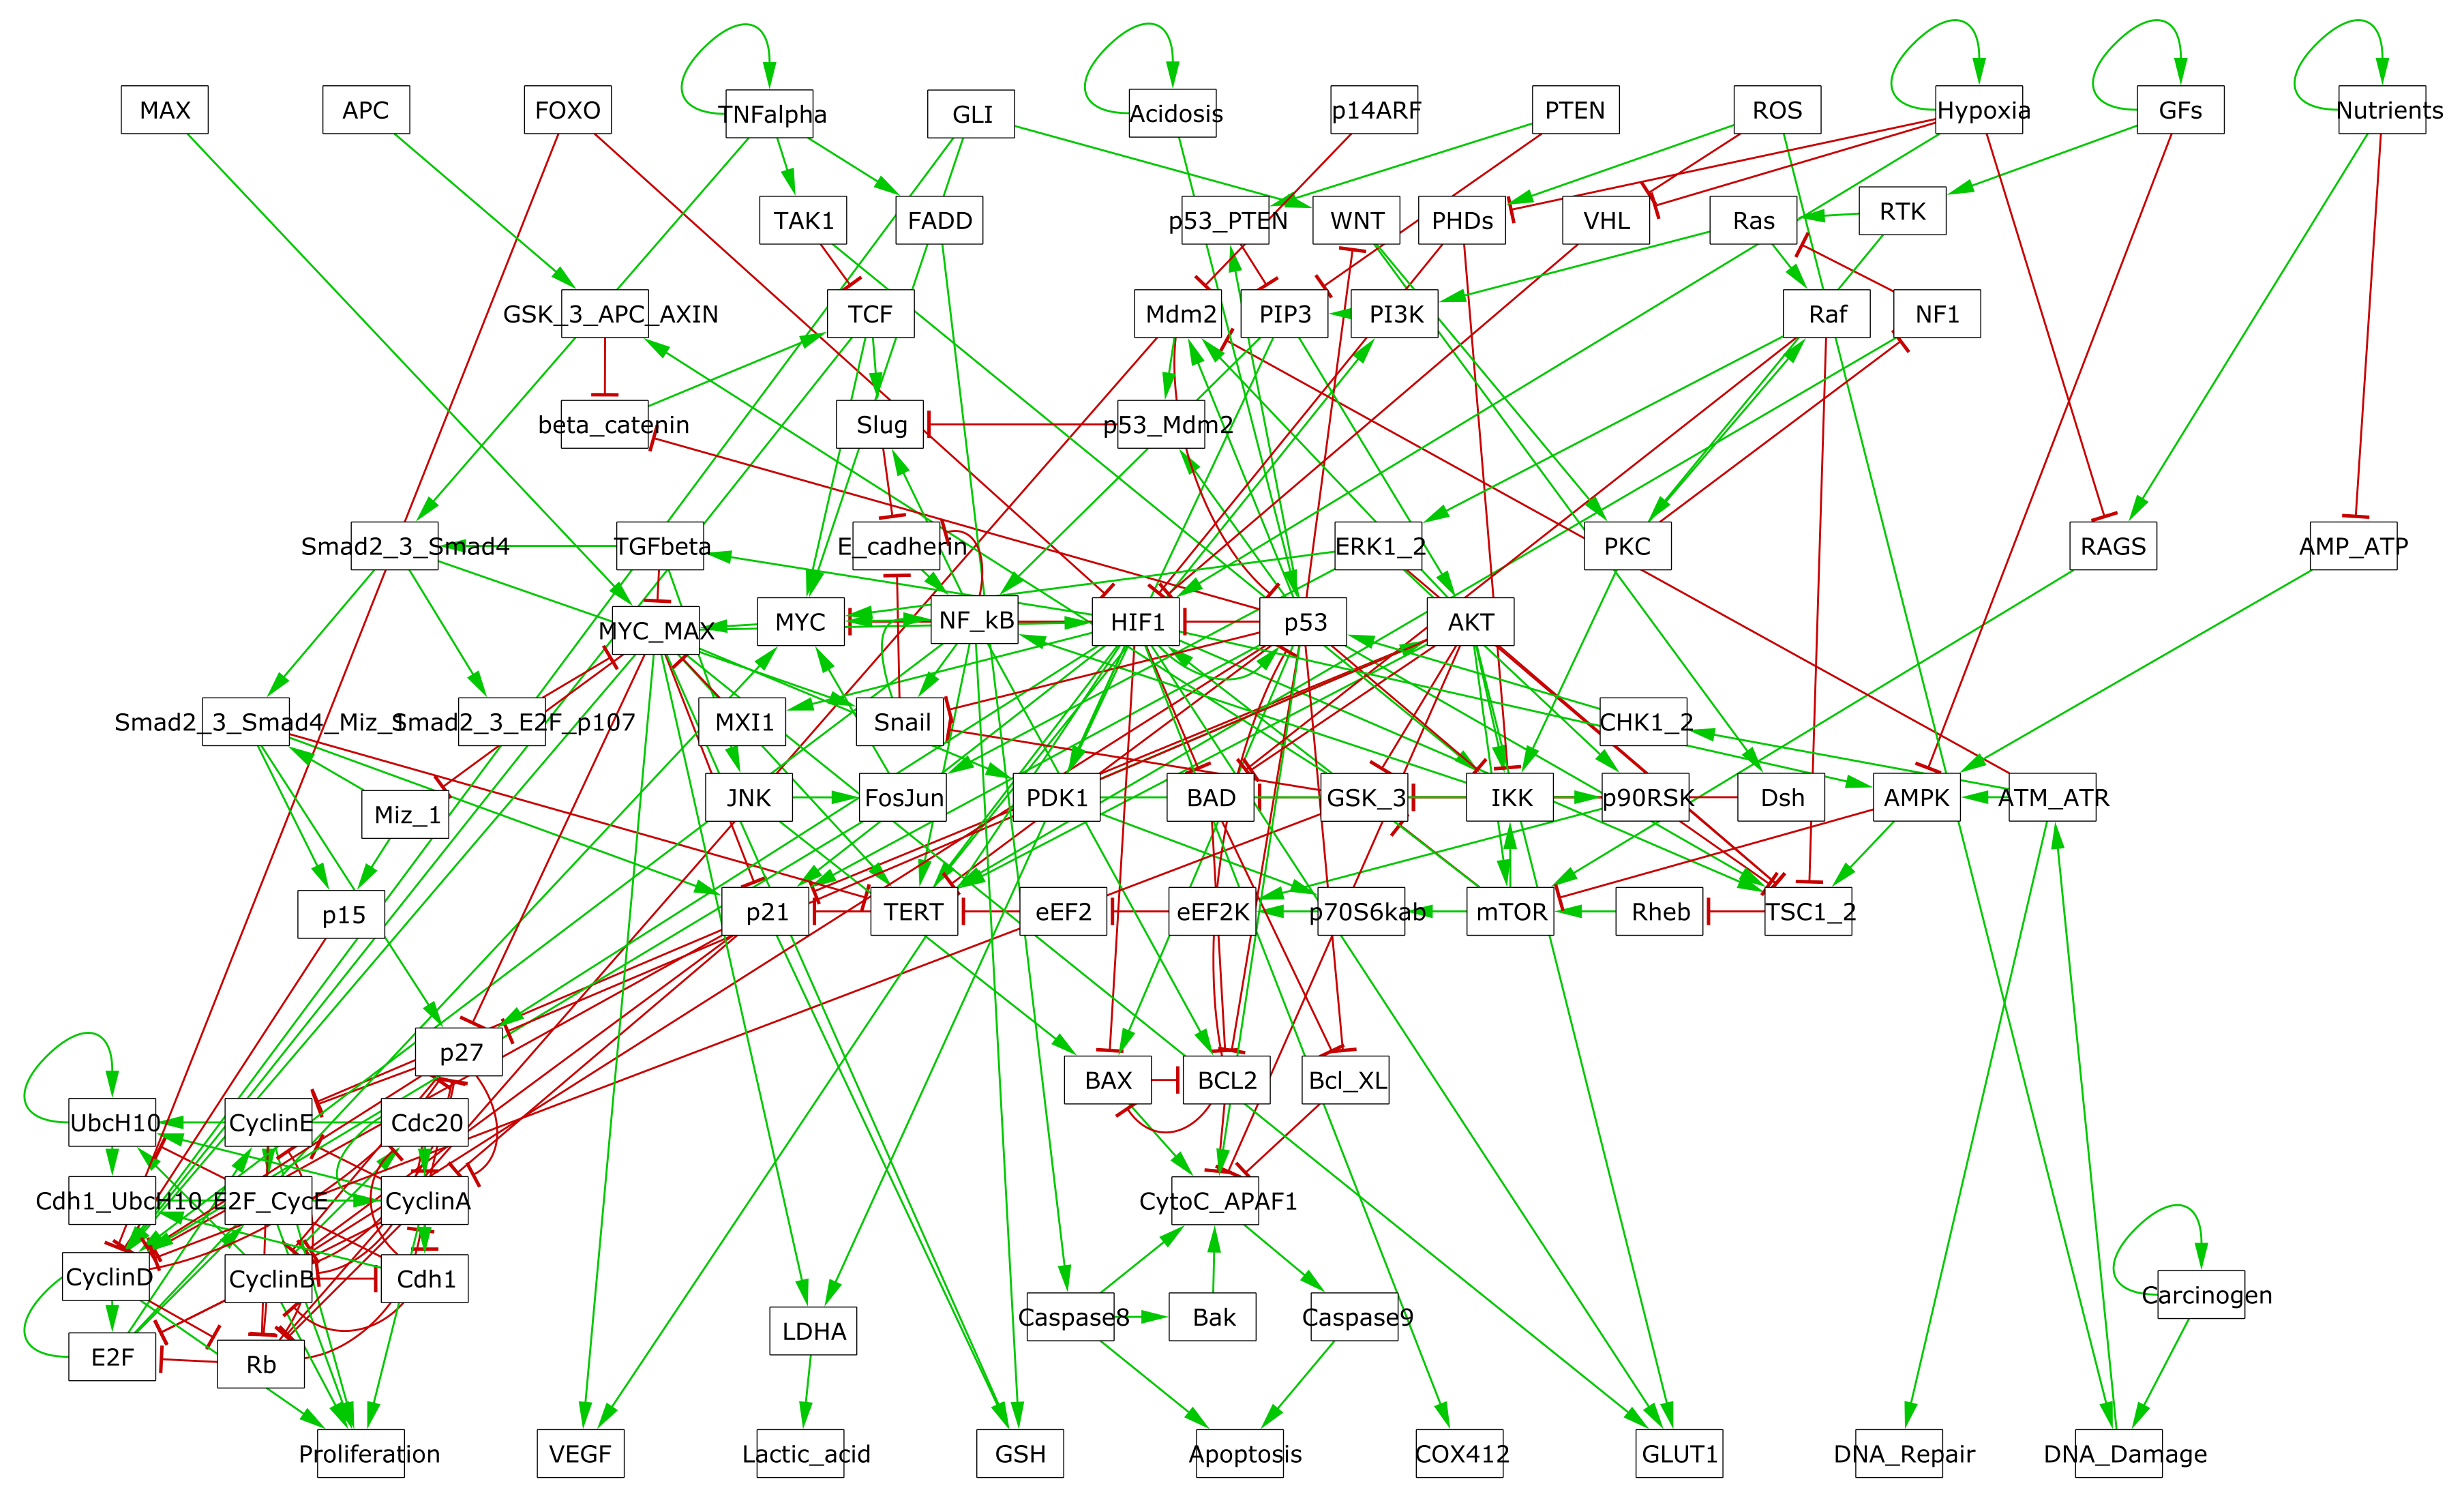
\includegraphics[width=0.9\linewidth]{fig/Fumia2013} 

}

\caption[Graphical abstract of PROFILE method to personalize logical models with omics data]{\textbf{GINSIM representation of the logical model
described in \citet{fumia2013boolean}.}}\label{fig:Fumia}
\end{figure}




\section{Extended logical model of cancer
pathways}\label{appendix-verlingue}

Another logical model of similar size and scope was also used, primarily
for the study of treatment responses. This model was built by Loïc
Verlingue, a medical oncologist and member of the laboratory and
preliminary versions of the model are described in
\citet{verlingue2016comprehensive} and \citet{verlingue2016silico}. One
of the interests of this model is that it has been designed with a more
clinical perspective, notably centred on the response to MTOR
inhibitors. In addition, it presents more biological read-outs used for
interpretation, and we will use mainly \emph{Proliferation} (also called
\emph{G1\_S} in the moel files to designate the associated stage of the
cell cycle), \emph{Apoptosis} and \emph{Quiescence} in particular. In
addition, being able to discuss and collaborate directly with the model
autor has helped to avoid potential errors in use.

\begin{figure}

{\centering \includegraphics[width=0.9\linewidth]{fig/Verlingue} 

}

\caption[Graphical abstract of PROFILE method to personalize logical models with omics data]{\textbf{GINSIM representation of the `Verlingue'
logical model described in \citet{verlingue2016silico}.}}\label{fig:Verlingue}
\end{figure}




\section{Logical model of BRAF pathways in melanoma and colorectal
cancer}\label{appendix-pantolini}

Here are some details about the regulations represented in Figure
\ref{fig:BRAF-model}. The MAPK pathway encompasses three families of
protein kinases: RAF, MEK, ERK. If RAF is separated into two isoforms,
CRAF and BRAF, the other two families MEK and ERK are represented by a
single node. When BRAF is inhibited, ERK can still be activated through
CRAF, and BRAF binds to and phosphorylates MEK1 and MEK2 more
efficiently than CRAF \citep{wellbrock2004raf}, especially in his
V600E/K mutated form. When PI3K/AKT pathway is activated, through the
presence of the HGF (Hepatocyte Growth Factors), EGF (Epidermal Growth
Factors) and FGF (Fibroblast Growth Factors) ligands, it leads to a
proliferative phenotype. The activation of this pathway results in the
activation of PDPK1 and mTOR, both able to phosphorylate p70 (RPS6KB1)
which then promotes cell proliferation and growth
\citep{uniprot2019uniprot}. There has been some evidence of negative
regulations of these two pathways carried out by ERK itself
\citep{lake2016negative}: phosphorylated ERK is able to prevent the
SOS-GRB2 complex formation through the activation of SPRY
\citep{edwin2009intermolecular}, inhibit the EGF-dependent GAB1/PI3K
association \citep{lehr2004identification} and down-regulate EGFR signal
through phosphorylation \citep{lake2016negative}. The model also
accounts for a negative regulation of proliferation through a pathway
involving p53 activation in response to DNA damage (represented by ATM);
p53 hinders proliferation through the activation of both PTEN, a PI3K
inhibitor, and p21 (CDKN1A) responsible for cell cycle arrest.

We hypothesize that a single network is able to discriminate between
melanoma and CRC cells. These differences may come from different
sources. One of them is linked to the negative feedback loop from ERK to
EGFR. As mentioned previously, this feedback leads to one important
difference in response to treatment between melanoma and CRC:
\(BRAF^{(V600E)}\) inhibition causes a rapid feedback activation of
EGFR, which supports continued proliferation. This feedback is observed
only in colorectal since melanoma cells express low levels of EGFR and
are therefore not subject to this reactivation
\citep{prahallad2012unresponsiveness}. Moreover, phosphorylation of
SOX10 by ERK inhibits its transcription activity towards multiple target
genes by interfering with the sumoylation of SOX10 at K55, which is
essential for its transcriptional activity \citep{han2018erk}. The
absence of ERK releases the activity of SOX10, which is necessary and
sufficient for FOXD3 induction. FOXD3 is then able to directly activate
the expression of ERBB3 at the transcriptional level, enhancing the
responsiveness of melanoma cells to NRG1 (the ligand for ERBB3), and
thus leading to the reactivation of both MAPK and PI3K/AKT pathways
\citep{han2018erk}. Furthermore, it has been shown that in colorectal
cells, FOXD3 inhibits EGFR signal \emph{in vitro} \citep{li2017foxd3}.
Interestingly, SOX10 is highly expressed in melanoma cell lines when
compared to other cancer cells. In the model, we define SOX10 as an
input because of the lack of information about the regulatory mechanisms
controlling its activity. The different expression levels of SOX10 have
been reported to play an important role in melanoma (high expression)
and colorectal (low expression) cell lines.

Besides a list of formalized biological assertions, retrieved from
literature, has been used during the model building to ensure the
consitency of the model with some qualitative behaviours. These
assertions, listed below, are all verified when the logical model is
simulated (details are available on the corresponding
\href{https://github.com/sysbio-curie/MaBoSS_test}{GitHub repository}):

\begin{itemize}
\tightlist
\item
  BRAF inhibition causes a feedback activation of EGFR in colorectal
  cancer and not in melanoma \citep{prahallad2012unresponsiveness}
\item
  MEK inhibition stops ERK signal but activates the PI3K/Akt pathway and
  increases the activity of ERBB3
  \citep{gopal2010basal, lake2016negative}
\item
  HGF signal leads to the reactivation of the MAPK and PI3K/AKT
  pathways, and resistance to BRAF inhibition \citep{wroblewski2013bh3}
\item
  BRAF inhibition in melanoma activates the SOX10/FOXD3/ERBB3 axis,
  which mediates resistance through the activation of the PI3K/AKT
  pathway \citep{han2018erk}
\item
  Overexpression/mutation of CRAF results in constitutive activation of
  ERK and MEK also in the presence of a BRAF inhibitor
  {[}\citet{manzano2016resistant}; johannessen2010cot{]}
\item
  Early resistance to BRAF inhibition may be observed in case of PTEN
  loss, or mutations in PI3K or AKT \citep{manzano2016resistant}
\item
  Experiments in melanoma cell lines support combined treatment with
  BRAF/MEK + PI3K/AKT inhibitors to overcome resistance
  \citep{manzano2016resistant}
\item
  BRAF inhibition (Vemurafenib) leads to the induction of PI3K/AKT
  pathway and inhibition of EGFR did not block this induction
  \citep{corcoran2012egfr}
\item
  Induction of PI3K/AKT pathway signaling has been associated with
  decreased sensitivity to MAPK inhibition \citep{corcoran2012egfr}
\end{itemize}

\section{Logical model of prostate cancer}\label{appendix-montagud}

In the context of the European project
\href{https://precise-project.eu/}{PRECISE} (Personalized Engine for
Cancer Integrative Study and Evaluation), focused on the integrative
study of prostate cancer, an adapted logical model has been built. This
prostate cancer model is initially based on the generic structure of the
Fumia model presented in section \ref{appendix-fumia}, which has been
considerably enriched and extended with genes and mechanisms specific to
prostate cancer such as ERG, SPOP or AR. The model contains 133 nodes
and 449 edges (Figure \ref{fig:Montagud}) and includes pathways like
androgen receptor and growth factor signalling, several signaling
pathways (Wnt, NFkB, PI3K/AKT, MAPK, mTOR, SHH), cell cycle,
epithelial-mesenchymal transition (EMT), Apoptosis, DNA damage, etc. The
model has 9 inputs (EGF, FGF, TGF beta, Nutrients, Hypoxia, Acidosis,
Androgen, TNF alpha and Carcinogen presence) and 6 outputs
(\emph{Proliferation}, \emph{Apoptosis}, \emph{Invasion},
\emph{Migration}, (bone) \emph{Metastasis} and \emph{DNA repair}).

\begin{figure}

{\centering \includegraphics[width=0.9\linewidth]{fig/Montagud} 

}

\caption[Graphical abstract of PROFILE method to personalize logical models with omics data]{\textbf{GINSIM representation of the `Montagud'
logical model of prostate cancer.}}\label{fig:Montagud}
\end{figure}




\chapter{About causality}\label{about-causality}

\section{Theoretical framework}\label{theoretical-framework}

\chapter*{References}\label{references}
\addcontentsline{toc}{chapter}{References}

\markboth{References}{References}

\setlength{\parindent}{-0.5in} \setlength{\leftskip}{0.5in}
\setlength{\parskip}{8pt}

\bibliography{bib/thesis.bib}

\end{document}
